\documentclass[12pt]{report}
\usepackage[danish]{babel}
\usepackage{microtype}
\usepackage[a4paper,top=3cm,bottom=3cm,left=1.5cm,right=1.5cm,marginparwidth=1.75cm]{geometry}
\usepackage{fancyhdr}
\usepackage{graphicx}
\usepackage{wrapfig}
\usepackage{index}
\usepackage{titlesec}
\usepackage{etoolbox}
\usepackage{amsmath}

\usepackage{lscape} % lig siden ned. 
\usepackage{longtable} % table
\usepackage{hyperref} % hyperlinks
\usepackage{xcolor}
\hypersetup{
	pdfborderstyle={/S/U/W 1},
    linkbordercolor=cyan, 
    colorlinks=true,
    citebordercolor=green,     % color of links to bibliography
    filebordercolor=magenta,   % color of file links
    urlbordercolor=cyan,       % color of external links
    linkcolor=black,
    filecolor=magenta,      
    urlcolor=blue,
}

\usepackage[utf8x]{inputenc}

\usepackage{array}
\usepackage[none]{hyphenat}

\makeindex
\pagestyle{fancy}
\fancypagestyle{plain}{
	\pagestyle{empty}
	\fancyhead[c]{hallo}
	\fancyfoot[c]{\raisebox{-6\baselineskip}{\thepage}}
	\fancyfoot[C]{\iffloatpage{}{\thepage}}
	}
\renewcommand{\headrulewidth}{0pt}
\renewcommand{\footrulewidth}{0pt}




\titleformat{\chapter}
  {\normalfont\LARGE\bfseries}{\thechapter}{1em}{}
\titlespacing*{\chapter}{0pt}{3.5ex plus 1ex minus .2ex}{2.3ex plus .2ex}
\makeatletter
\patchcmd{\chapter}{\if@openright\cleardoublepage\else\clearpage\fi}{}{}{}


\usepackage{listings}
\usepackage{color}

\definecolor{dkgreen}{rgb}{0,0.6,0}
\definecolor{gray}{rgb}{0.5,0.5,0.5}
\definecolor{mauve}{rgb}{0.58,0,0.82}

\lstset{frame=tb,
  language=Java,
  aboveskip=1mm,
  belowskip=1mm,
  showstringspaces=true,
  columns=flexible,
  basicstyle={\small\ttfamily},
  numbers=none,
  numberstyle=\tiny\color{gray},
  keywordstyle=\color{blue},
  commentstyle=\color{dkgreen},
  stringstyle=\color{mauve},
  breaklines=true,
  breakatwhitespace=true,
  tabsize=1
}
\renewcommand{\thechapter}{\Roman{chapter}}




\begin{document}
\title{MMMI}
\author{By projektgruppe 02 }
\date{Marts 25 - 2019}
\pagestyle{fancy}






\begin{titlepage}

\clearpage
\maketitle
\thispagestyle{empty}









\end{titlepage}

\chapter{Resume}
Omfatter resuméet:\\
Den behandlede problemstilling - hvad blev der arbejdet med og hvorfor?\\
Fremgangsmåden - anvendte metoder - hvordan blev der arbejdet med det? \\
(hvordan angreb I problemet og hvordan realiserede I løsningen (hvem, hvad, hvornår og hvorfor)\\
Hovedresultater og konklusioner  – hvad kom der ud af arbejdet?\\
\begin{Large}
(max  1 side)
\end{Large}

Indeholder forord hensigten med rapporten, målgruppe, forhistorie, anerkendelser, afleveringsdato samt underskrifter af alle projektdeltagere?\\
Bemærk: Projektdeltagernes aktive deltagelse i projektforløbet anerkendes gensidigt ved projektdeltagernes underskrifter i rapporten. 

\clearpage

\tableofcontents
\clearpage

\chapter{Læsevejledning}
Denne rapport er skrevet ud fra antagelsen om at læseren har en grundlæggende forståelse for programmering og software engineering, som svarer til gruppens eget vidensniveau. 
Det er meningen, at rapporten skal kunne læses igennem fra indledning til perspektivering. 
Indledning og konklusion kan i øvrigt læses i sammenhæng for at få en klar forståelse for projektets mål og de opnåede resultater. 
Ved læsning af første og anden iteration er de begge delt op i lignende afsnit. 
Afsnittene kan læses for en iteration ad gangen eller det ene afsnit fra første iteration og det samme afsnit fra anden iteration. 
Anden del af rapporten er om, 
hvad gruppen har lært og hvordan gruppen har arbejdet og hvordan samarbejdet har fungeret. For at se kildekoden anbefales det at se Javadoc i projektet. 
Der er også en brugervejledning der kort fortæller hvordan programmet skal bruges. 
Referencer til gruppens eget arbejde, som ikke kan ses på den pågældende side, 
kan findes i det interne bilag, 
mens øvrige bilag vil være i eksterne bilag. Dette er gældende for alle afsnit af rapporten.\\


Beskriver redaktionelt skriveprocessen og ansvarsområder i skriveprocessen?\\
Ansvarsområder kan fx beskrives på fx følgende form:

\section{Ordliste}
Er der en kort beskrivelse af de fagtermer der bruges gennem rapporten?

\newpage
Giver indledningen et overblik over projektet og baggrunden for det?\\
Giver indledningen et resume af den udleverede case?\\
Indeholder indledningen problemformuleringen, jfr. inceptiondokumentet?\\
Beskriver indledningen formålet med projektet?\\ Er formålet i overensstemmelse med hensigten med 2. semester? \\
Beskriver indledningen målene med projektet? Udtrykker målene specifikke, målbare resultater, jfr. inceptionsdokumentet? \\
Er målene i overensstemmelse med de overordnede mål for 2. semester som udtrykt i studieordningens kap. 9 og de mere specifikke mål for projektet, som udtrykt i fagbeskrivelsen for SI2-PRO?

\section{Problemformulering}


Salget af KMD førte til etableringen af det kommunale IT-fællesskab KOMBIT\footnote{\url{ https://www.kombit.dk/KOMBIThistorie}}, som arbejder på at sikre de bedste og billigste IT-løsninger set ud fra kommunernes behov. De kommunale behov blev tidligere varetaget af KMD, men som resultat af deres monopolbrud, valgte KOMBIT at udbyde disse behov til forskellige IT-leverandører . Dette skabte muligheden for at EG Team Online kunne træde ind på det kommunale IT-marked.
Allerede i 2005 præsenterede EG Team Online, dengang kendt som Team Online, deres første store system inden for velfærdsområdet, Sensum Bosted, dengang kendt som Bosted System. Dette system var revolutionerende inden for lokale bosteder og institutioner som arbejder med patientbehandling. Ved at digitalisere journaler og andre former for papirarbejde, blev socialarbejdernes arbejdsbyrde mindsket og deres effektivitet øget. I 2007 modtog Team Online ansvaret for it-løsninger hos Fyns Amt bo- og aktivitetsstedet Lindebjerg. Efterfølgende har virksomheden udviklet sig til at være en leverandør inden for innovativ teknologi med speciale i løsninger, der understøtter det samlede behov i den offentlige og private social- og sundhedssektor.\\ \\
I 2018 blev GDPR indført af EU-kommissionen, hvilket gjorde at den danske regering tilpassede den danske datalovgivning til GDPR. Denne ratificering betød at alle IT-selskaber skulle følge nye regler angående håndtering af persondata. Derfor er EG Team Online ved at tilpasse deres produkt.\\
\\
Gruppen har fået udleveret en case som omhandler et system udviklet af EG Team Online. Virksomheden ønsker en belysning af tre moduler: planlægning, sagsudredning og dagbogen. Gruppen har diskuteret afgrænsning i forhold til de specifikke moduler, hvor der var en interesse i hvordan flere roller i systemet interagerer med hinanden. I forhold til persondatalovgivningen har virksomheden beskrevet en dataafgrænsning i casen hvor de beskriver hvem der må kunne interagere med hvad i systemet. På baggrund af de strengere regler om persondata, blev det nødvendigt at opdatere systemet.
 

\textbf{\\Gruppen kom frem til følgende hovedspørgsmål.}\\ \\
\noindent\fbox{%
    \parbox{\textwidth}{%
Hvordan kan et program håndtere flere roller uden at de interagerer med hinandens data samt hvilke sikkerhedsforanstaltninger ligger til grund for at beskytte data?
    }%
}
 \textbf{\\DeleSpørgsmål\\}\\
På baggrund af den centrale problemstilling er der blevet udformet følgende underspørgsmål:\\ 
\begin{itemize}
\item Hvad definerer roller?
\item Hvilket ansvarsområder ligger til grund for rollerne?
\item Hvilken persistent data bearbejdes?
\item Hvordan håndterer systemet flere roller?
\item Hvordan håndteres roller med flere ansvarsområder?
\item Hvilke sikkerhedsforanstaltninger er der i forhold til data afgrænsningen?
\item Hvordan sikres det at aktøren kun har adgang til det aktøren har brug for? 
\end{itemize}
Gruppen lavede en analyse af den udleverede case. På baggrund af analysen dannede gruppen et overblik over problemstillingen. Analysen belyser de forskellige aktørers roller og ansvarsområder. EG-teamet ønsker en belysning af 3 moduler, hvor gruppen valgte dataafgrænsningen i forhold til sikkerhedsforanstaltninger, der adskiller de forskellige roller.
Under inceptionsfasen (Life Cycle Objectives) bliver målene sat for, hvordan projektet skal udformes og hvilke forudsætninger skal der tages højde for. Nogle af målene for inceptionsfasen kan være aktørliste, brugsmønster og kravspecifikationer. 
Dette skal skabe grundlaget for videre arbejde i elaborationsfasen, samt danne overblik over projektcasen. 



\section{Metoder}
Er metoden i det samlede projekt beskrevet?\\
Er det beskrevet hvordan UP og Scrum kombineres i projektet, samt hvilke fordele og ulemper der er ved det?\\

\subsection{Indledning til metoder}
Giver indledningen en introduktion til  afsnittet?\\
\subsection{Metoder}
Er metoden i det samlede projekt beskrevet?\\
Er det beskrevet hvordan UP og Scrum kombineres i projektet, samt hvilke fordele og ulemper der er ved det?\\
\subsection{Planlægning}
Er planlægningen af elaborationsfasen og de enkelte iterationer beskrevet.\\
Er backlogs beskrevet?\\
Er rollefordelingen i projektgruppen beskrevet?\\
Er ceremonierne beskrevet?\\
Er scrum-buts beskrevet?\\
Bygger planen på prioriteringen af kravene efter inceptionsfasen.\\


\chapter{Metoder}
Metoder er en vigtig del af et projekt, som udformer væsentlige resultater og holder styr på fremgangen. Der vil under metodeafsnittet beskrives de metoder som har været anvendt under hele projektet, som f.eks. UP, kanban og par produktion. (Afsnit 7.1) \\
Unified Process (forkortet UP) er en iterativ, inkrementel og brugsmønster-drevet software udviklingsproces. UP bliver brugt med en kombination af den agile metode Scrum der er en trinvis og iterativ tilgang til udarbejdelse af et produkt. Gruppens anvendelse og kombination af disse beskrives. (Afsnit 7.2) \\
Til sidst bliver der uddybet beskrivelserne af Scrum’s forskellige egenskaber som f.eks. Scrum backlog, ceremonier m.m. (Afsnit 7.3) \\

\section{Samlede metoder}
Under starten af projektet blev der holdt et møde omkring hvordan og hvilket metoder der kunne og skulle anvendes. Under dette møde blev der forklaret hvilke metoder hvert enkelt gruppemedlem anvendte i deres projekt. Til det blev der diskuteret hvilke metoder der med fordel kunne anvendes i nuværende projekt, hvor der blev udvalgt de mest væsentlige og effektive metoder. Ydermere blev der gjort krav til at anvende UP og Scrum som læner sig op ad den agile metodologi. \\
\textbf{ Unified process (UP)} har været anvendt igennem hele projektet der er blanding af agile og planlægnings metode. Den består af forskellige faser, dvs. forberedelsesfase (inception), etableringsfase (elaboration), konstruktionsfase (construction) og overdragelsesfase (transition). Projektetrammen begrænser projektet i det omfang at forberedelsesfasen og etableringsfasen er de faser der skal fokuseres på. Dette fokus er bestemt for at tilrettelægge et projekt uden at fokus går på programmering selv.\\ 
\emph{Inceptionsfasen} er en kort fase der har til formål at give et overblik over de indhentede krav. Hovedtrækkene i fasen handler om at:\\
\begin{itemize}
\item Forstå hvad der skal bygges
\item Identificere de væsentlige funktioner i systemet, og beskrive dem ved at bruge brugsmønstre
\item Identificere projektets plan og kritiske risici
\item Udvælge udviklingsværktøjer til selve udviklingsprocessen
\end{itemize}
\emph{Elaborationsfasen} handler om at analysere problemdomænet og tilegne sig en endelig forståelse af hele systemet. Hovedtrækkene handler om at: \\
\begin{itemize}
\item Designe brugsmønstrene
\item Producere en arkitektonisk baseline for systemet som skal bygges
\end{itemize}
\textbf{Kanban} er en mindre formel metode end Scrum der bliver brugt til at holde styr på hvilke opgaver der skal laves og hvem der arbejder på opgaverne gennem hele projektet. Formålet med at anvende kanban i projektet har været at holde styr på de opgaver der skulle bearbejdes i løbet hver iteration. Den har fungeret effektivt i forhold til opdeling af opgaverne, hvor hvert par kunne blive tildelt en opgave. Til fordel for kanban blev værktøjet GitKranken Glo brugt som et virtuelt whiteboard for at holde styr på de forskellige opgaver og milepæle. \\
\\
\textbf{Par produktion} er en agil metode, beskrivelsen af definitionen kan findes i bilag … under metodeafsnittet. \\
Metoden er blevet anvendt under hele projektet, som har haft den fordel at udarbejdelsen af opgaverne blev mere effektive og produktive. Samtidigt blev der holdt styr på de opgaver der skulle arbejdes på hver uge. 
\\ \\
\textbf{Scrum} er en agil metode, beskrivelsen af Scrum kan findes i bilag … under metodeafsnittet.
I projektgruppen er der blevet besluttet at bruge dele af Scrum, der består af roller, herunder et team som består af gruppemedlemmerne. Ceremonier herunder daglige Scrum møder. Artefakter herunder produkt backlog. Det er ikke blevet fundet nødvendigt at anvende hele Scrum frameworket er ikke nok mennesker til at kunne bruge Scrum i det omfang at kunne benytte hele Scrum. Ydermere har vi ikke den nødvendige viden til at kunne benytte det, f.eks. har vi ikke en Scrum master eller product owner. \\

\subsection{Kombination af Scrum og UP}
Igennem hele projektforløbet er der blevet anvendt Unified Process. \\
Det betyder at der arbejdes i faser, hvor gruppen ender med at være igennem Inception- og elaborationsfasen. \\
Efter introduktionen til Scrum, er der i gruppen blevet valgt at kombinere noget af Scrum metoden med resten af metoderne. \\
Der anvendes Scrumbot, hvilket betyder at der er lavet en liste over spints og de iterationer som der udarbejdes igennem sprintene.\\
\subsection{Planlægning}
Er planlægningen af elaborationsfasen og de enkelte iterationer beskrevet.\\
Er backlogs beskrevet?\\
Er rollefordelingen i projektgruppen beskrevet?\\
Er ceremonierne beskrevet?\\
Er scrum-buts beskrevet?\\
Bygger planen på prioriteringen af kravene efter inceptionsfasen.\\

Hvis der indgår et teoretisk problem: Omfatter hovedteksten et teori-afsnit?\\
\section{Indlening til hovedafsnit}
Indeholder indledningen en overordnet introduktion til afsnittet?\\
\section{Første iteration}
\subsection{Indledning til første iteration}
Formålet med elaborationsfasen er at skabe en interaktiv udvikling af produktet MMMI´s\footnote{{mangfoldig manager management instruments}} funktionalitet. Denne udvikling sker på baggrund af inceptionsfasen\footnote{{Bilag : Inceptionss dokumentet}}, hvor der blev opstillet en række krav til MMMI-projektet.  For at kunne nå de mål bliver der lagt lavet nogle mindre iterationer her under krav, analyse, design, kode og test som arbejdes med ud fra de overordnede kravspecifikationer. Målet er at får en funktionel kode færdig til elaborationsmilepælen. 



\section{Overordnet kravspecifikation (resume, opdateret)}
Indeholder afsnittet et opdateret resumé  af systemafgrænsningen fra inceptionsdokumentet.
\section{Detaljeret kravspecifikation}
Omfatter den detaljerede kravspecifikation\\
Detaljeret brugsmønsterdiagram (hvis relevant)\\
Detaljerede brugsmønsterbeskrivelser\\
Detaljerede beskrivelser af supplerende krav Fx organiseret efter FURPS+\\

\section{Analyse}
Omfatter afsnittet overvejelser, beslutninger og resultater vedr.\\
Den statiske side af analysemodel\\
Den dynamiske side af analysemodel\\

\section{Design}
Omfatter afsnittet overvejelser, beslutninger og resultater vedr.\\
Softwarearkitektur\\
Subsystemdesign\\
Den statiske side af designmodel\\
Den dynamiske side af designmodel\\
Design af persistens\\
Databasedesign\\

\section{Implementering}
Omfatter afsnittet overvejelser, beslutninger og resultater vedr.\\  konvertering fra design til kode illustreret gennem udvalgte centrale eksempler, samt andre vigtige implementeringsbeslutninger
Omfatter afsnittet implementering af database.



\subsection{Find sag metoden}
Under Department.java har vi en metode 
\subsubsection{Problem: }
En aktør skal kunne finde en sag samt få denne sag vist. Sagen skal findes ved hjælp at enten sagsnummer, cpr-nummer eller navn. 
\subsubsection{Løsning: }
For at finde en sag skal der første laves en liste over sagerne der er inde for den gældende afdeling har. 
Der bliver lavet en metode search der søger gennem alle de sager afdelingen har,
Herefter skal der findes en match på om sagen har enten matchende sagsnummer, cpr-nummer eller navn. 
\begin{figure}[h]
\begin{lstlisting}

    public List<Case> search(String searchWord) {

        List<Case> listCases = new ArrayList<>();

        for (Case searchCase : caseMap.values()) {
            if (searchCase.getRegardingCitizen().getCprNumber().equalsIgnoreCase(searchWord)
                    || searchCase.getCaseNumber().equalsIgnoreCase(String.valueOf(searchWord))
                    || searchCase.getRegardingCitizen().getName().equalsIgnoreCase(searchWord)) {
                listCases.add(searchCase);
            }
        }

        return listCases;
    }


\end{lstlisting}
\caption{kode : seartch}
\label{kode:Search}
\end{figure}



\subsubsection{Evaluering:}
Metoden virker når der kun er kendskab til et map men skal laves om når der skal søges i databasen efter den gældende sag.


\section{Test}
Omfatter afsnittet en beskrivelse af de udførte test samt resultatet af dem.\\
Er der medtaget resultater både fra iteration 1 og fra iteration 2?\\


Omfatter diskussionen hvad der er opnået, og hvad der ikke er opnået i projektet i forhold til det forventede som beskrevet i indledningen. \\
Hvad er styrkerne og svaghederne ved jeres resultater?\\
Kunne I have opnået bedre resultater?\\

\chapter{Konklusion}
Opsummerer konklusionen resultaterne og diskussionen af dem og giver det på problemformuleringen? \\

\chapter{Perspektivering}
Den nuværende fase som projektet befinder sig i er Elaborationsfasen (slutning af elaborationsfasen). Gruppen har arbejdet i 2. iteration med at få implementeret væsentlige brugsmønstre, som f.eks. find en sag eller finde en borger der er tilknyttet en sag, og oprettelse af en sag baseret på forskellige formular. \\
Det næste skridt i projektet er konstruktionsfasen der har til formål at udarbejde og implementere den manglende funktionalitet f.eks. behandle sag, tildeling af sag og dagbog, samtidig med at lave test, som gøre produktet klar til kunden. Dette kan gøres igennem 2 – 3 iterationer, hvor 1. iteration ville handle om at få optimeret kode i forhold til det der er i forvejen samt færdiggøre funktionaliteten. I 2. iteration af konstruktionsfasen ville der blive fokuseret på at få implementeret den resterende funktionalitet som f.eks. at afdelingslederen har mulighed for at tilde sager til sagsbehandlere. I 3. iteration lave en endelig version af systemet, med en brugergrænseflade der både er brugervenlig og funktionel og som er klar til test. Til sidst når projektet når transationsfasen er det til formål udgiver produktet til kunden, hvor så man får feedback og kan så justere og finpudse de resterende påpegninger til systemet. \\
Hvis projektet skulle bygges igen, med en realistisk tidsramme og med den viden som gruppen har tilegnet sig, så ville det gøres på følgende måde. Der ville med fordel kunne laves brugsmønstre og til det lave en overordnet kravspecifikation med væsentlige detaljerede brugsmønstre. Efterfølgende ville der blive udarbejdet et analyseklassediagram over alle de klasser og funktioner fundet i de detaljerede brugsmønstre og dermed udarbejde et designklassediagram til brug for implementering. Idet ville et component diagram også blive udarbejdet i forhold til at vise hvordan systemet er opbygget så der er bedre forståelse for forskellige komponenter. Til sidst begynder 1. iteration med at udarbejde funktionaliteten generelt og i 2. iteration udarbejde et databasedesign og database implementering og brugergrænseflade som en klar pakke til at blive sendt ind i en konstruktionsfase. I konstruktionsfasen ville produktet blive mere dybdegående udarbejdet og optimeret og lave en brugervenlig grænseflade igennem 2 – 3 iterationer og samtidig gøre den klar til levering for kunden til test. \\



Er litteratur angivet på en anerkendt form? \\
Er alle former for litteratur som bøger, artikler og hjemmesider medtaget? \\
Er der kildehenvisninger i teksten? \\
Materiale som gruppen ikke selv har fremstillet i dette projekt skal være angivet med kilde! \\
Er alle kildehenvisninger i teksten anført på samme måde? \\
Er der kildeangivelser på figurer, grafer etc. som projektgruppen ikke selv har frembragt? \\

\newpage

\chapter{Procesrapport}

\section{Læring og refleksion}

\section{Projektarbejde}

\section{Identifikationg, analyse og bearbejdning af problemer}

\section{Projektforløb}

\subsection{Formidling og kommunikation}

\subsection{Samarbejde i gruppen}

\subsection{Samarbejde med vejleder}








\chapter{Kildekode}
For at se gruppens javadoc gå til: \\
\url{https://github.com/Diplom-Software2018/Anden-semester/tree/gh-pages/ProjektMappen/MMMI/dist/javadoc}\\
For at se javadocs skal branchen hentes og ses der igennem.

Er der en kortfattet brugervejledning?

\chapter{Projektlog}
Er der en adresse på og et link til projektloggen i Github?
\clearpage
\thispagestyle{plain}{
\fancyhead{} }
\pagenumbering{Roman}

\chapter{Interne bilag}
er kontrolskemaet udfyldt?
\pagenumbering{roman}
\section{Projektforslag}
\begin{figure}[hb]
\begin{center}
  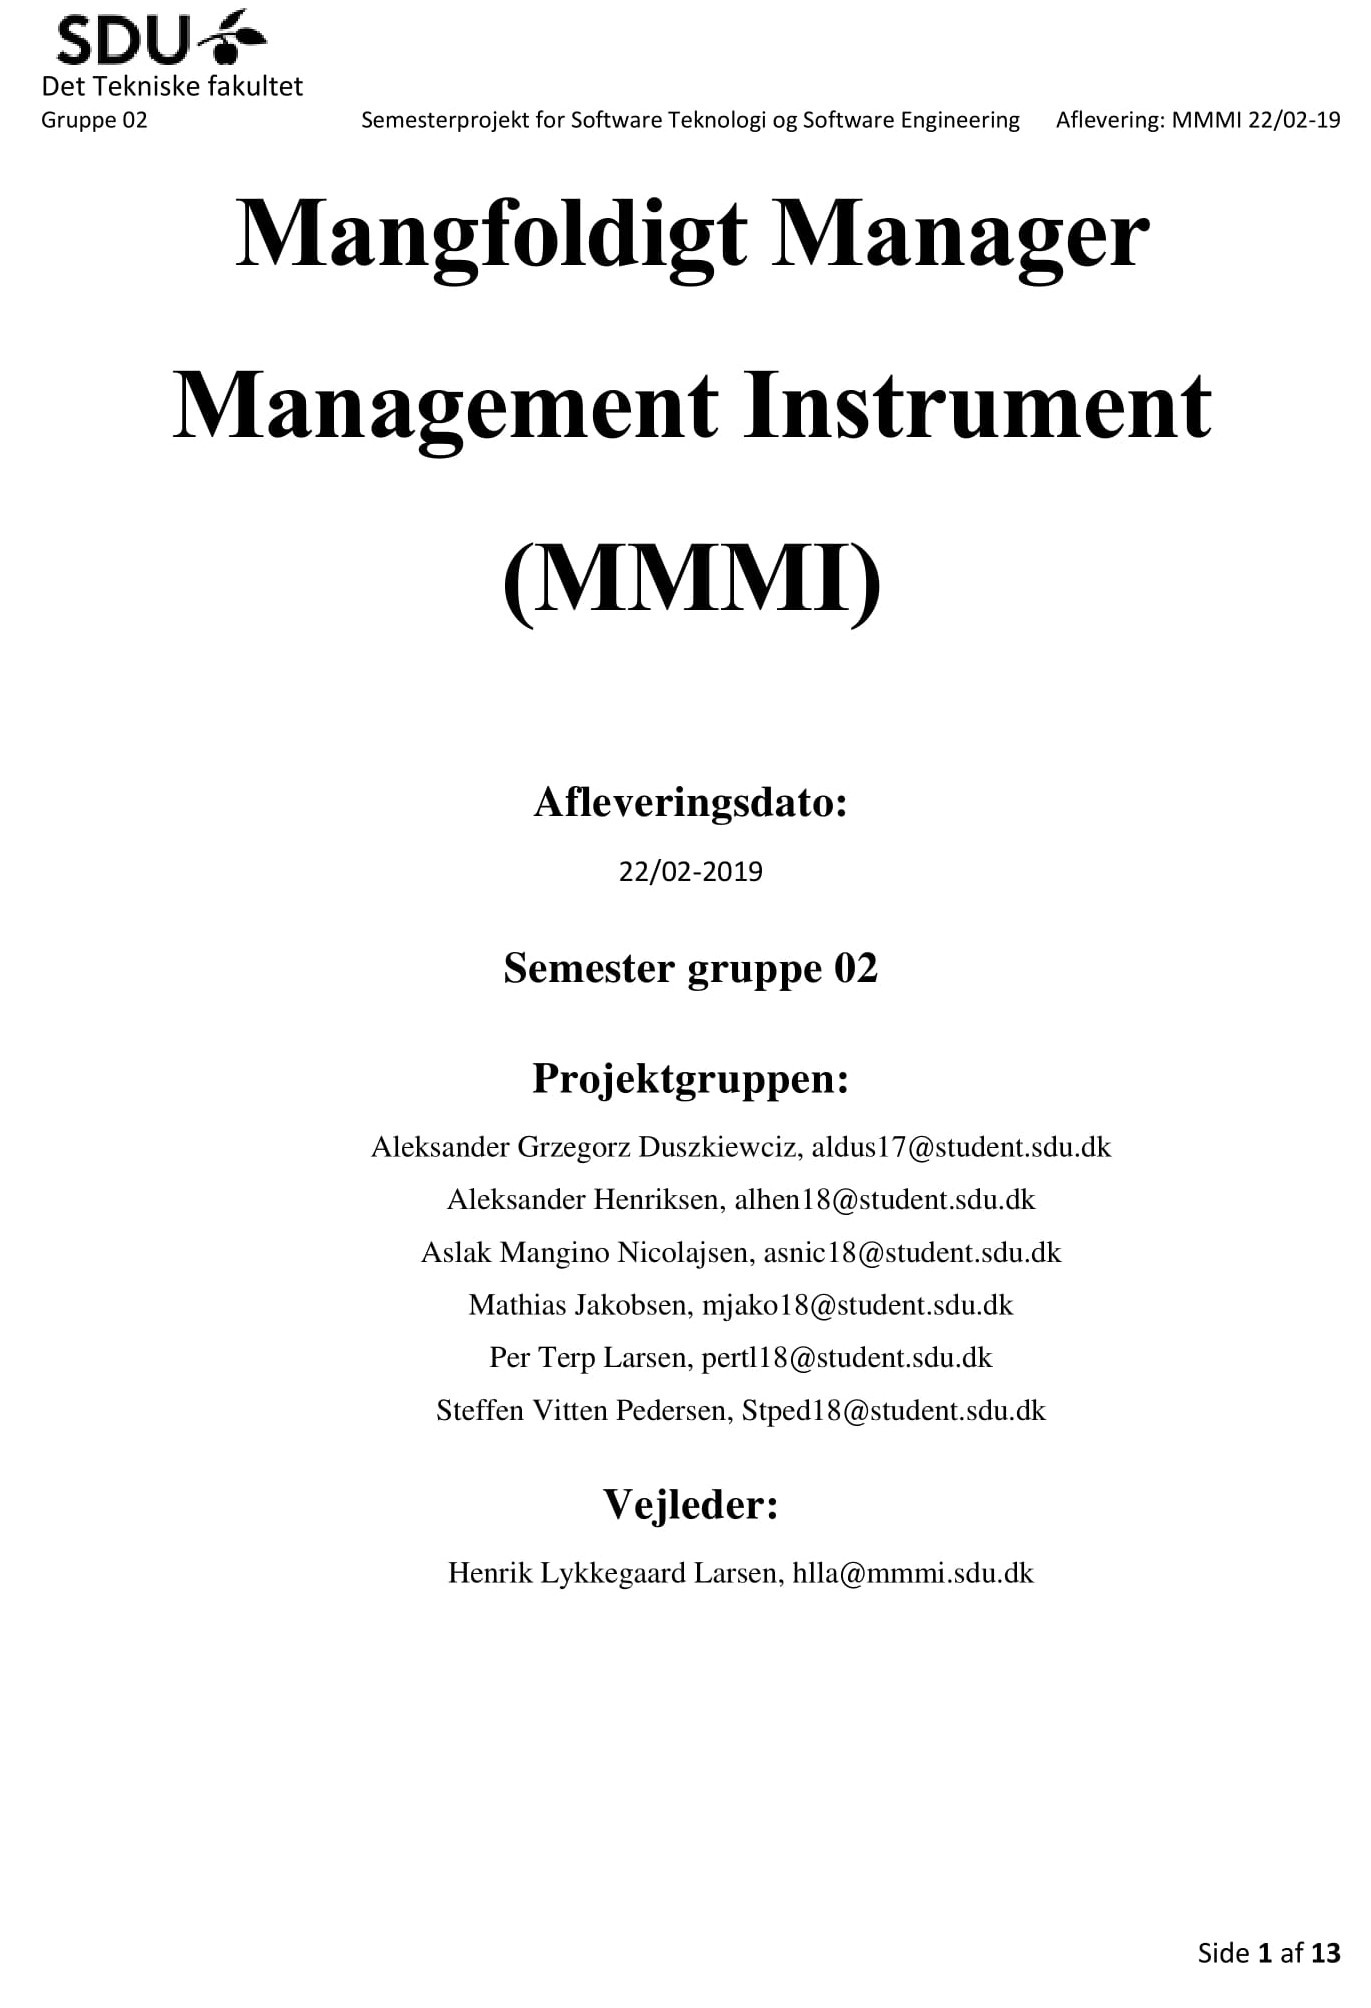
\includegraphics[scale = 0.33]{./PNG/Projektforslag/Projektforslag-01.jpg} 
\end{center}
\end{figure}

\begin{figure}[hb]
  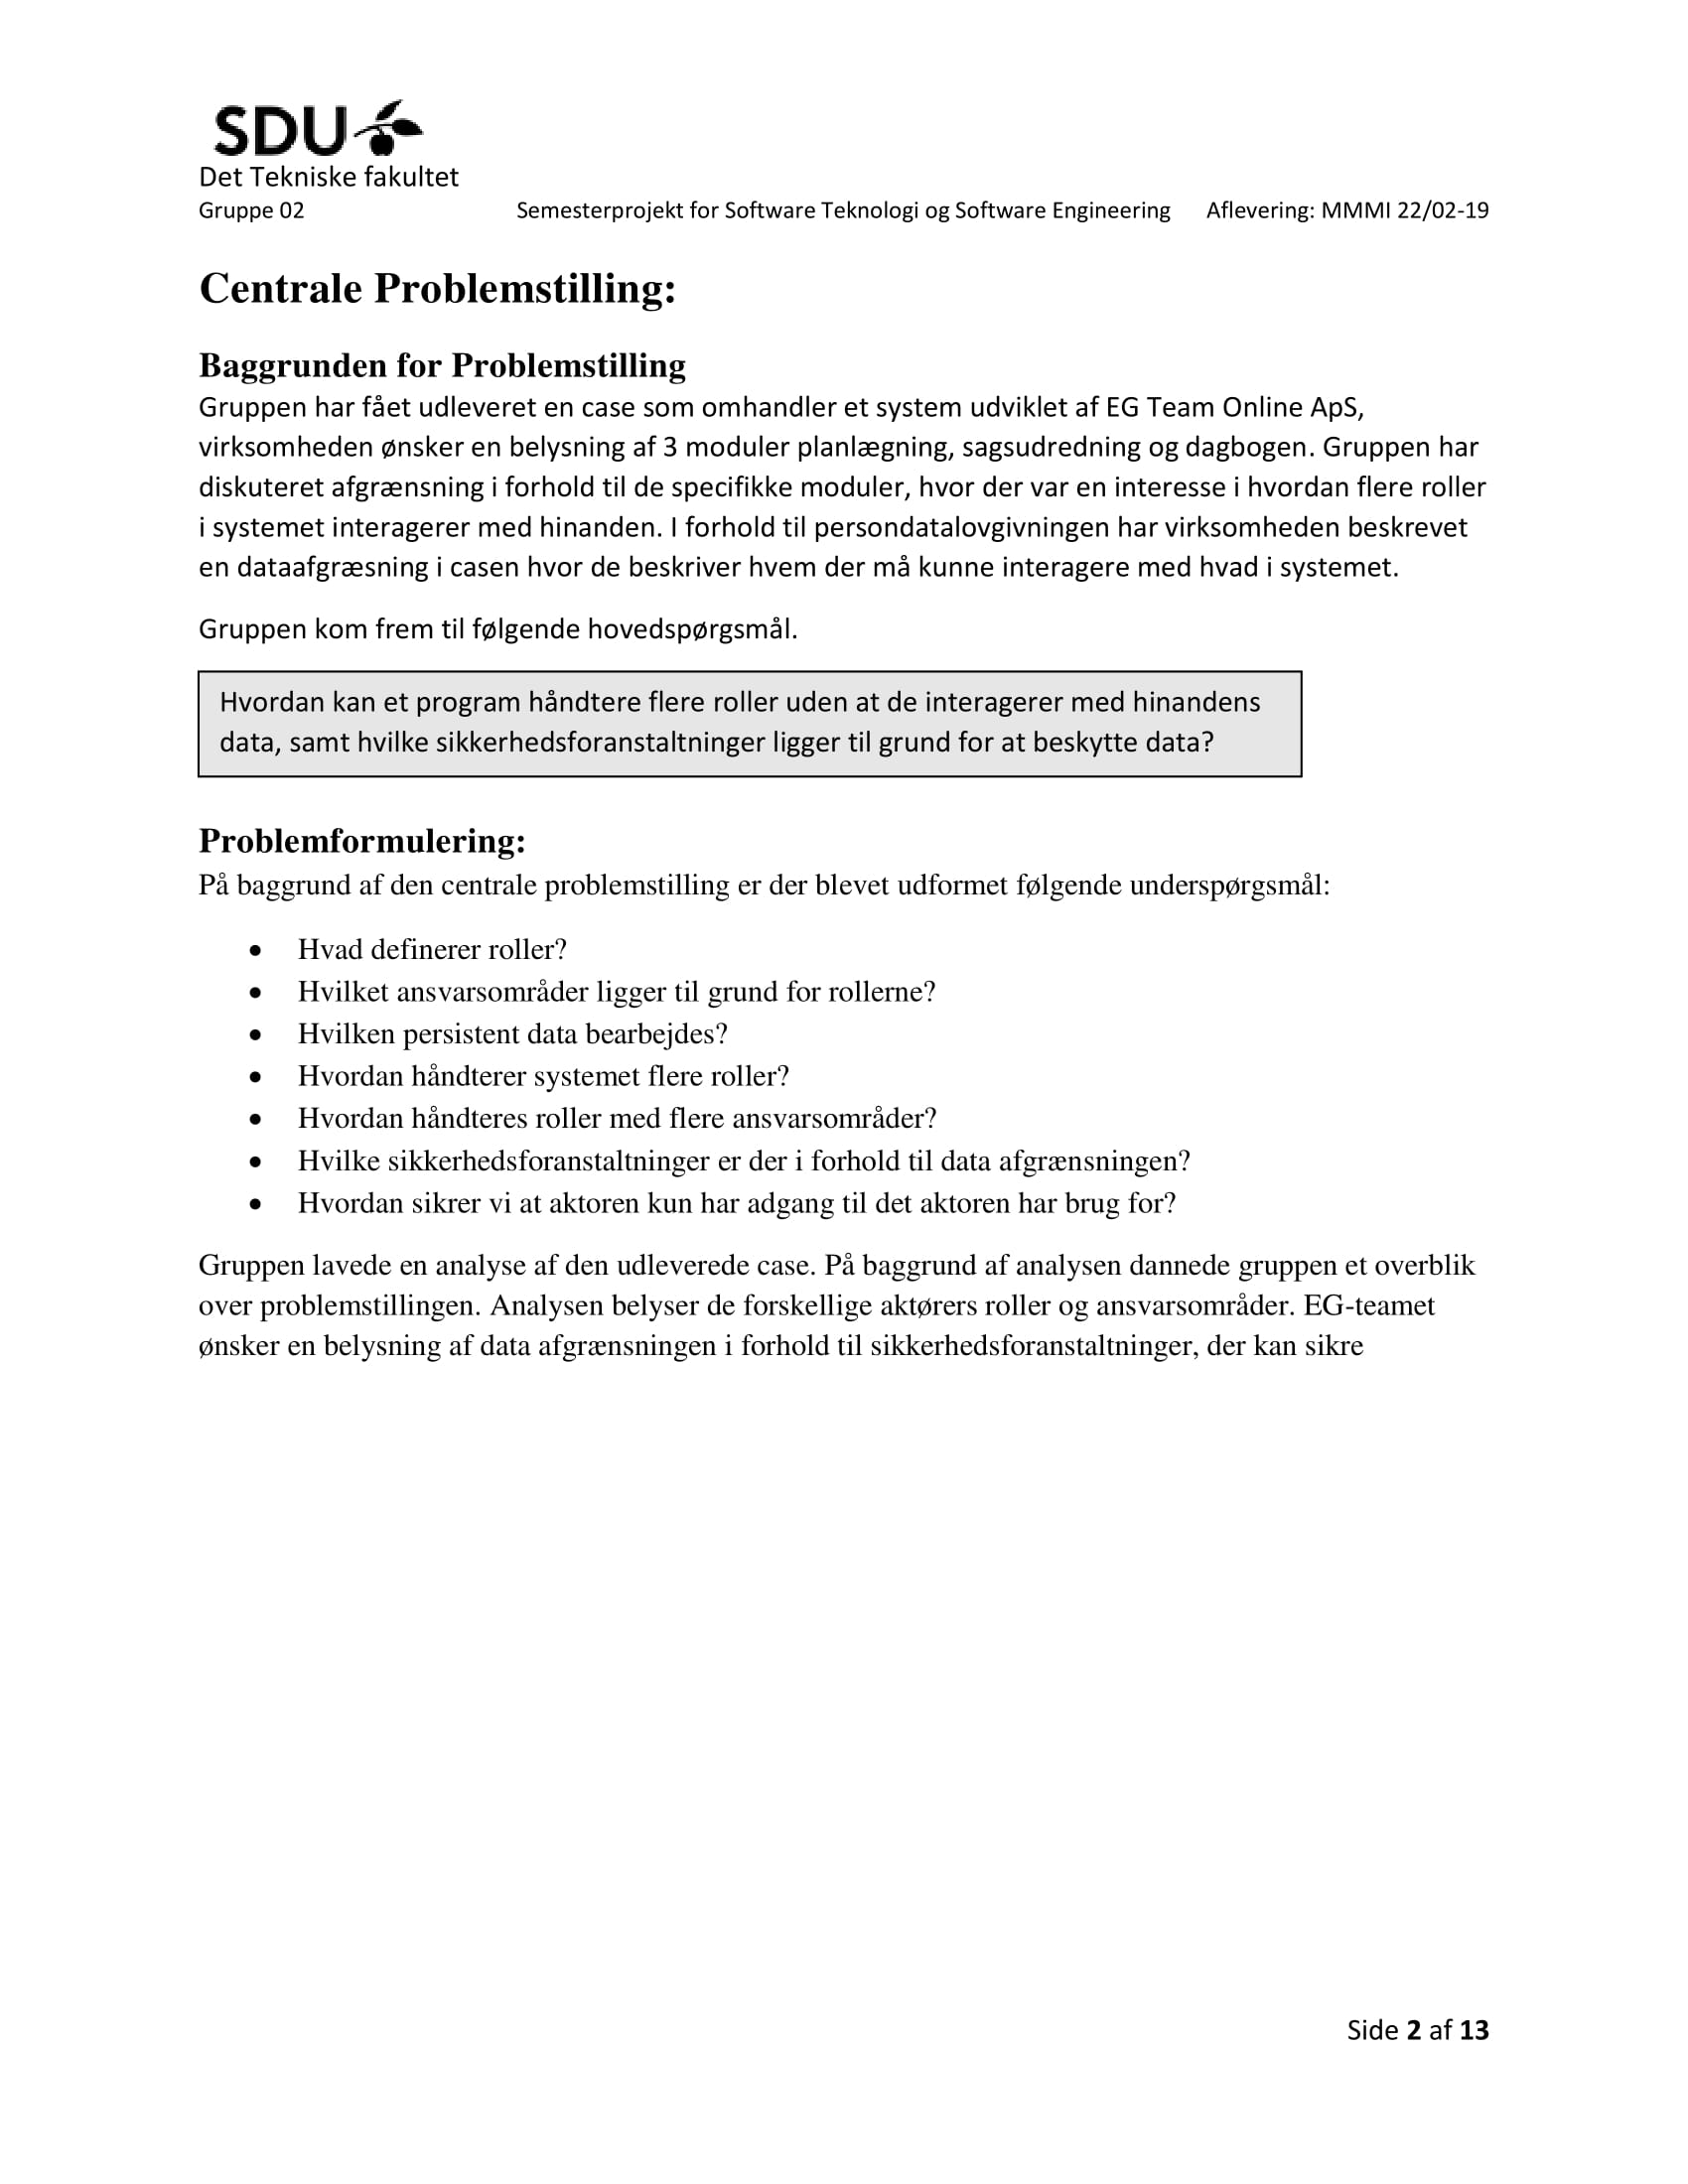
\includegraphics[scale = 0.33]{./PNG/Projektforslag/Projektforslag-02.jpg} 
\end{figure}

\begin{figure}[hb]
  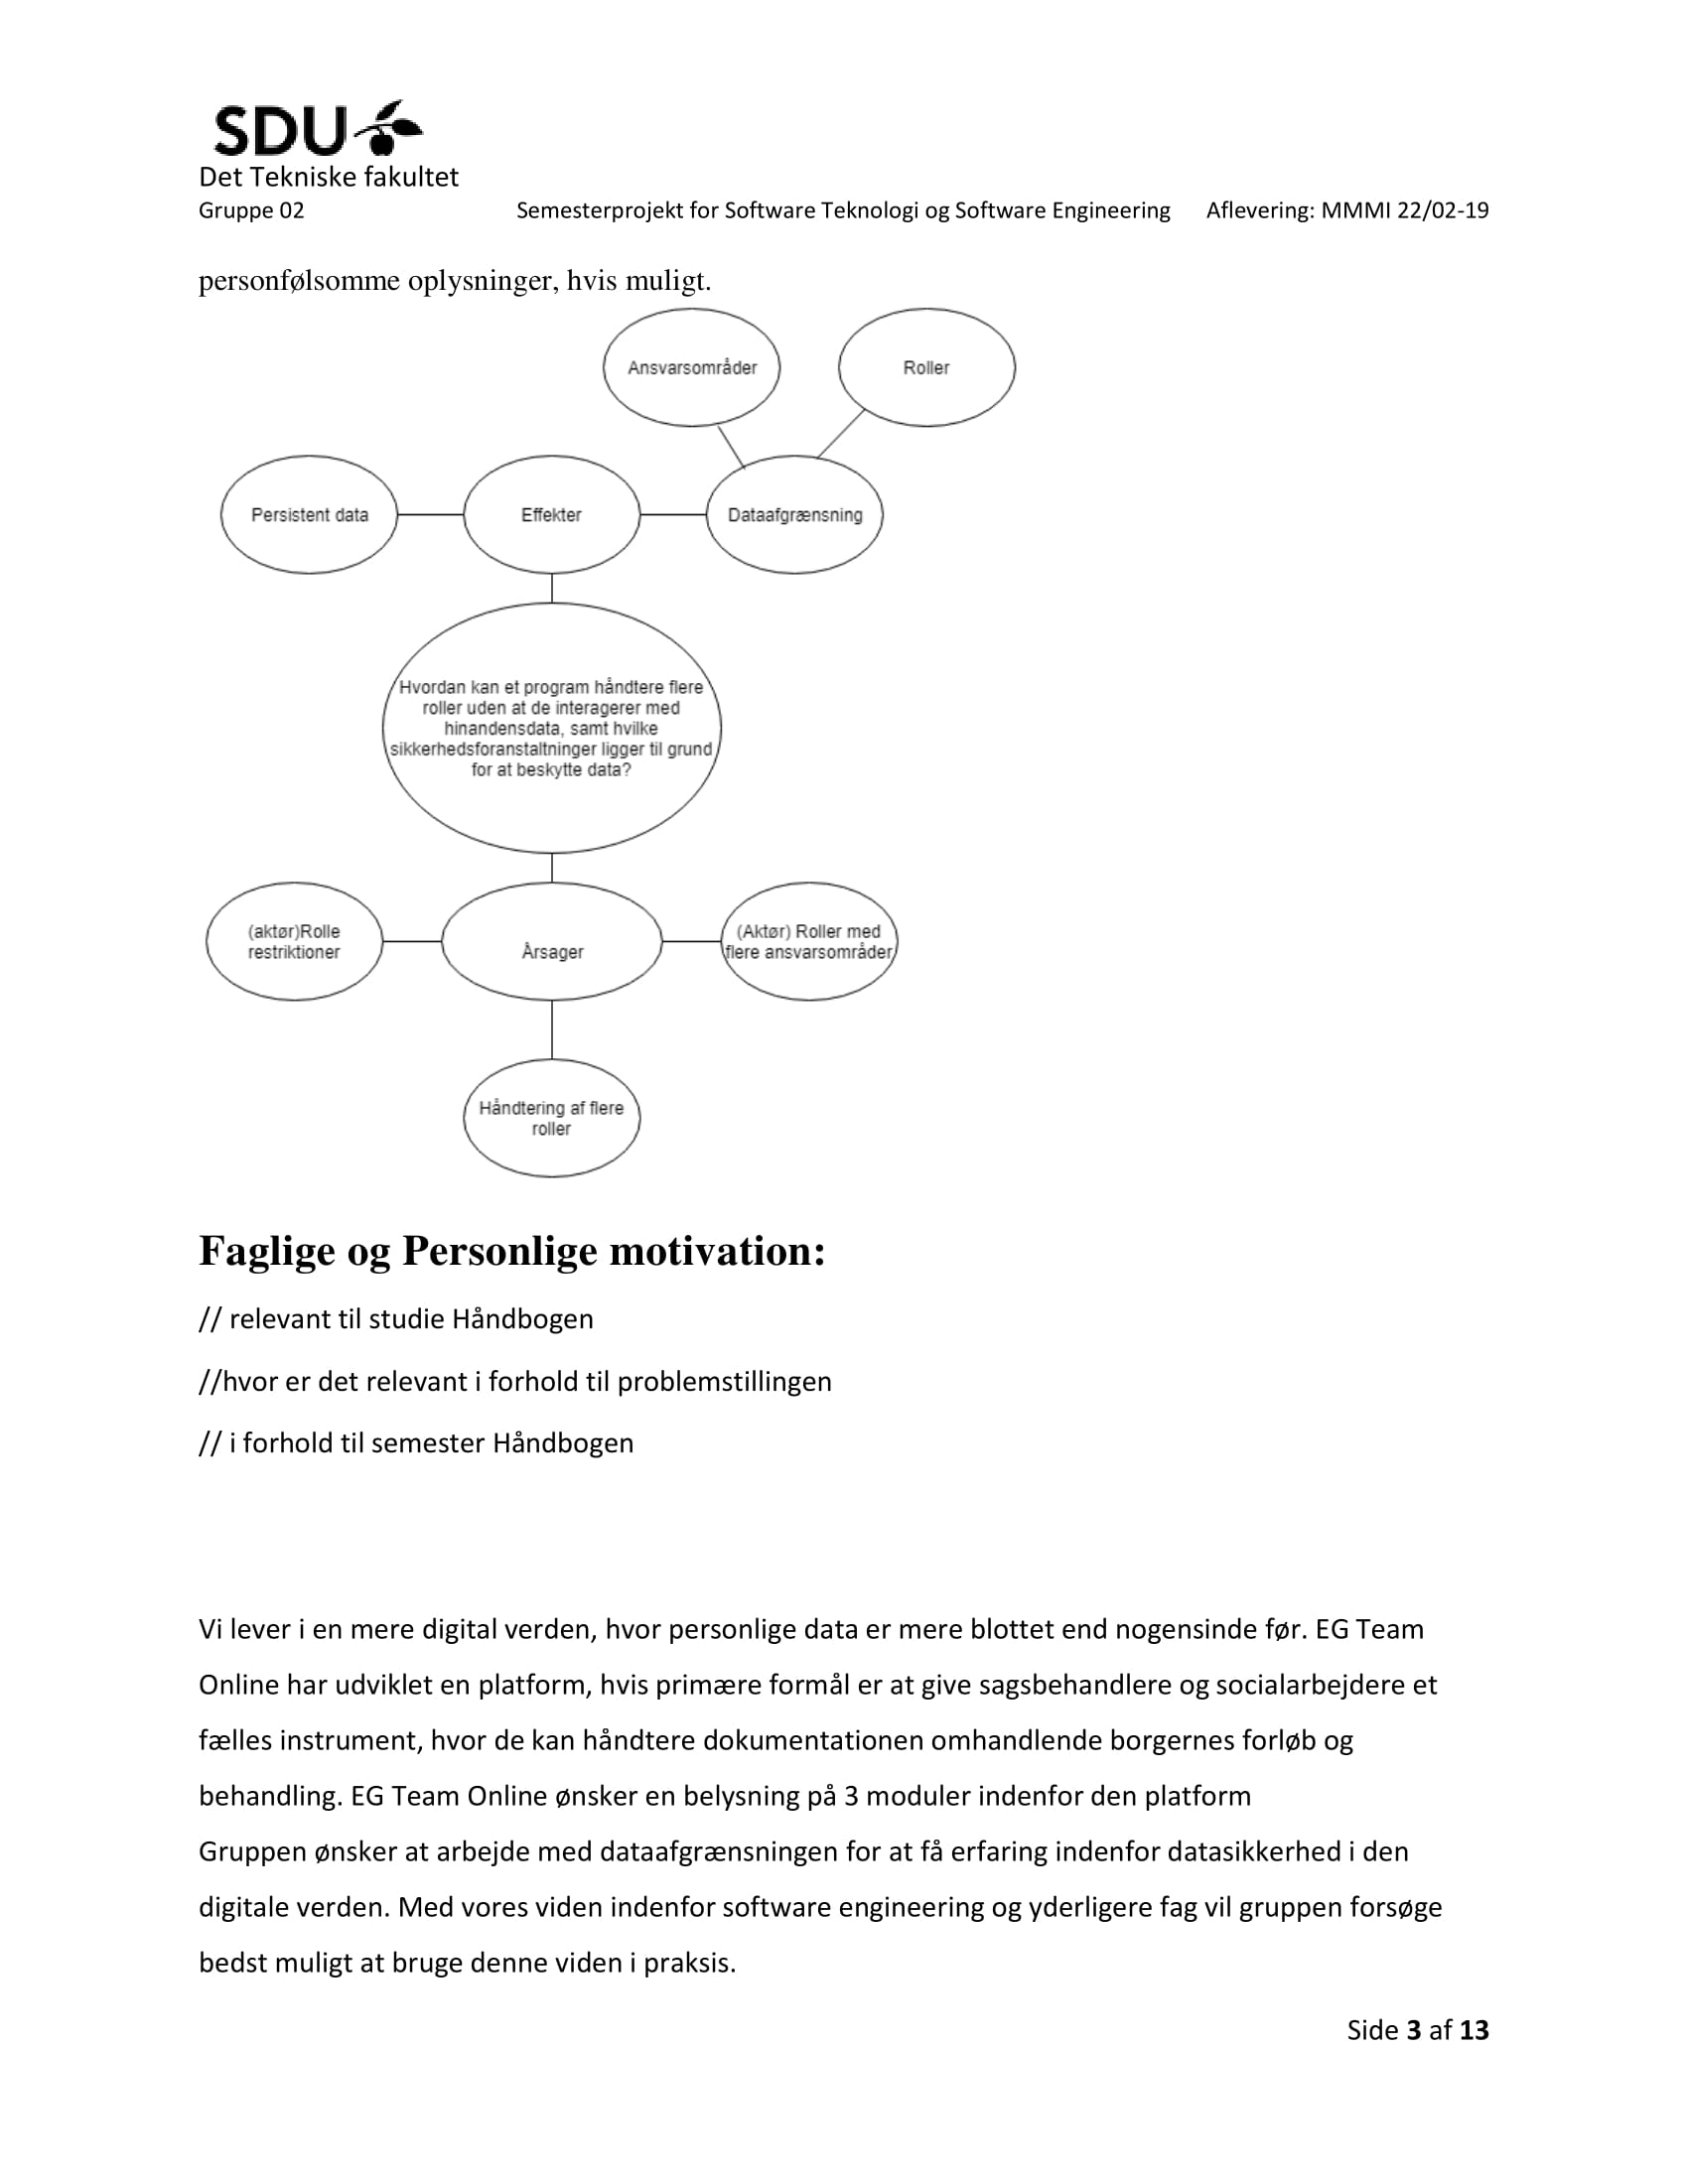
\includegraphics[scale = 0.33]{./PNG/Projektforslag/Projektforslag-03.jpg} 
\end{figure}

\begin{figure}[hb]
  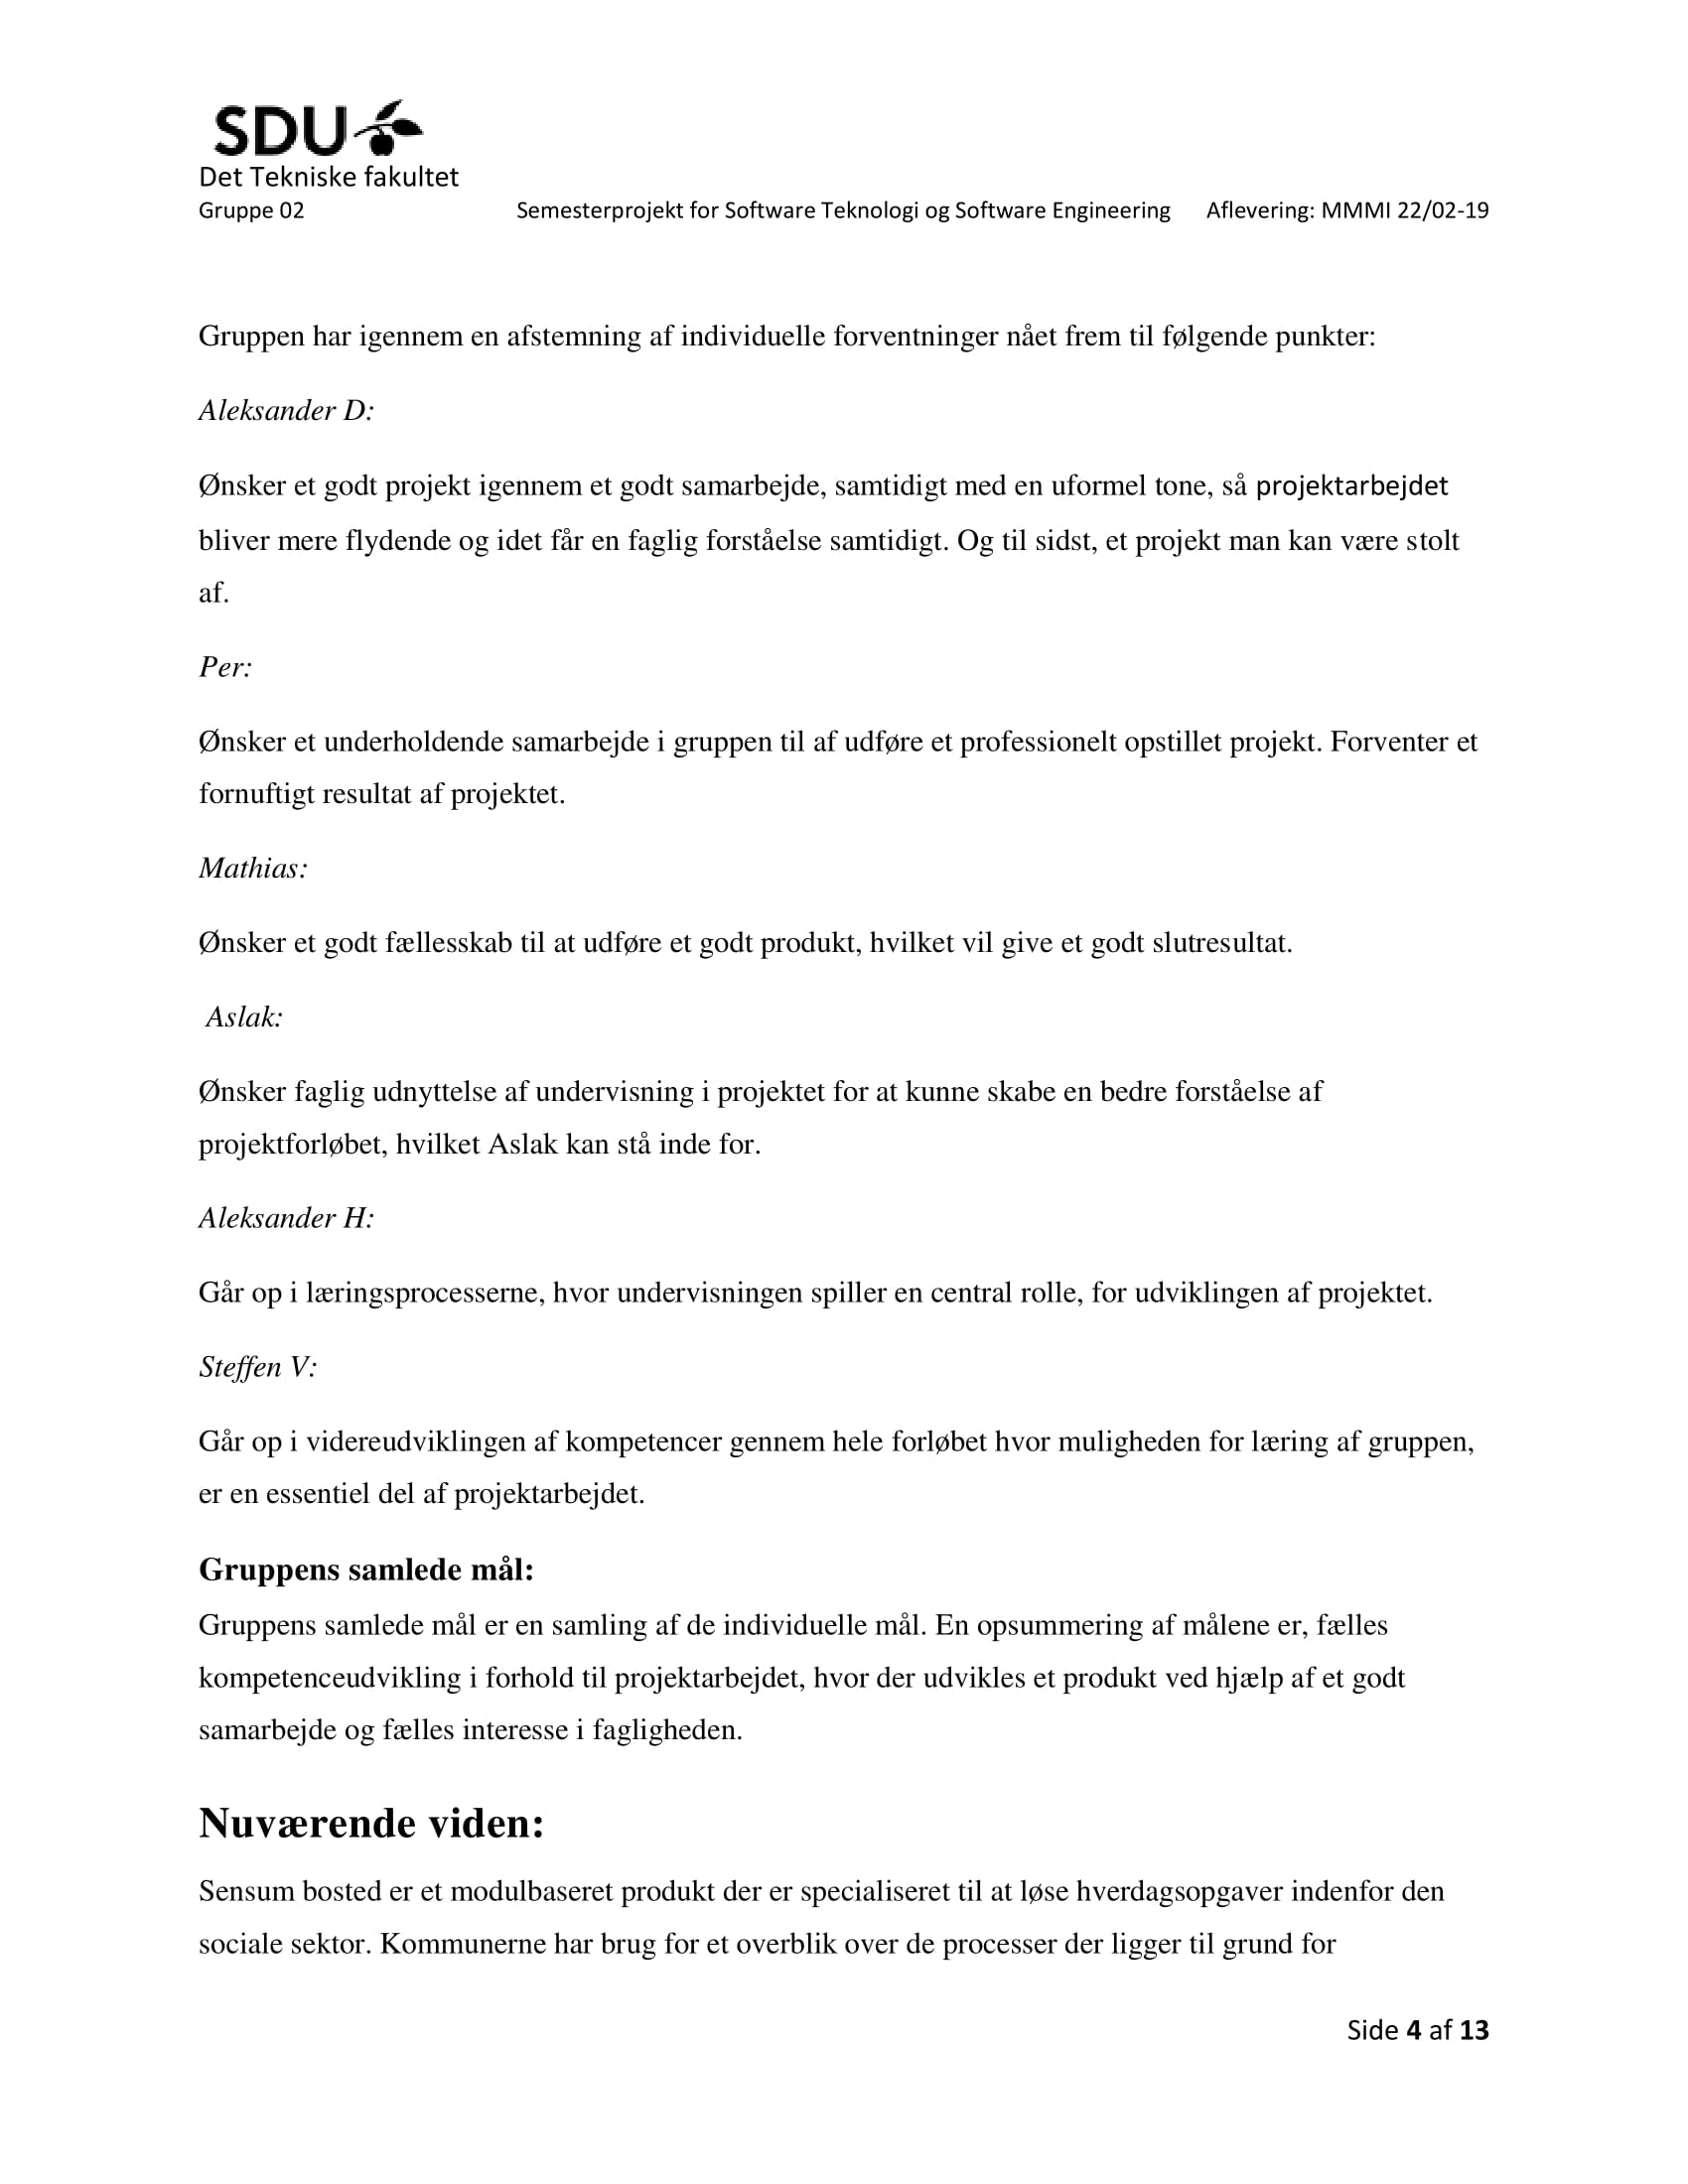
\includegraphics[scale = 0.33]{./PNG/Projektforslag/Projektforslag-04.jpg} 
\end{figure}

\begin{figure}[hb]
  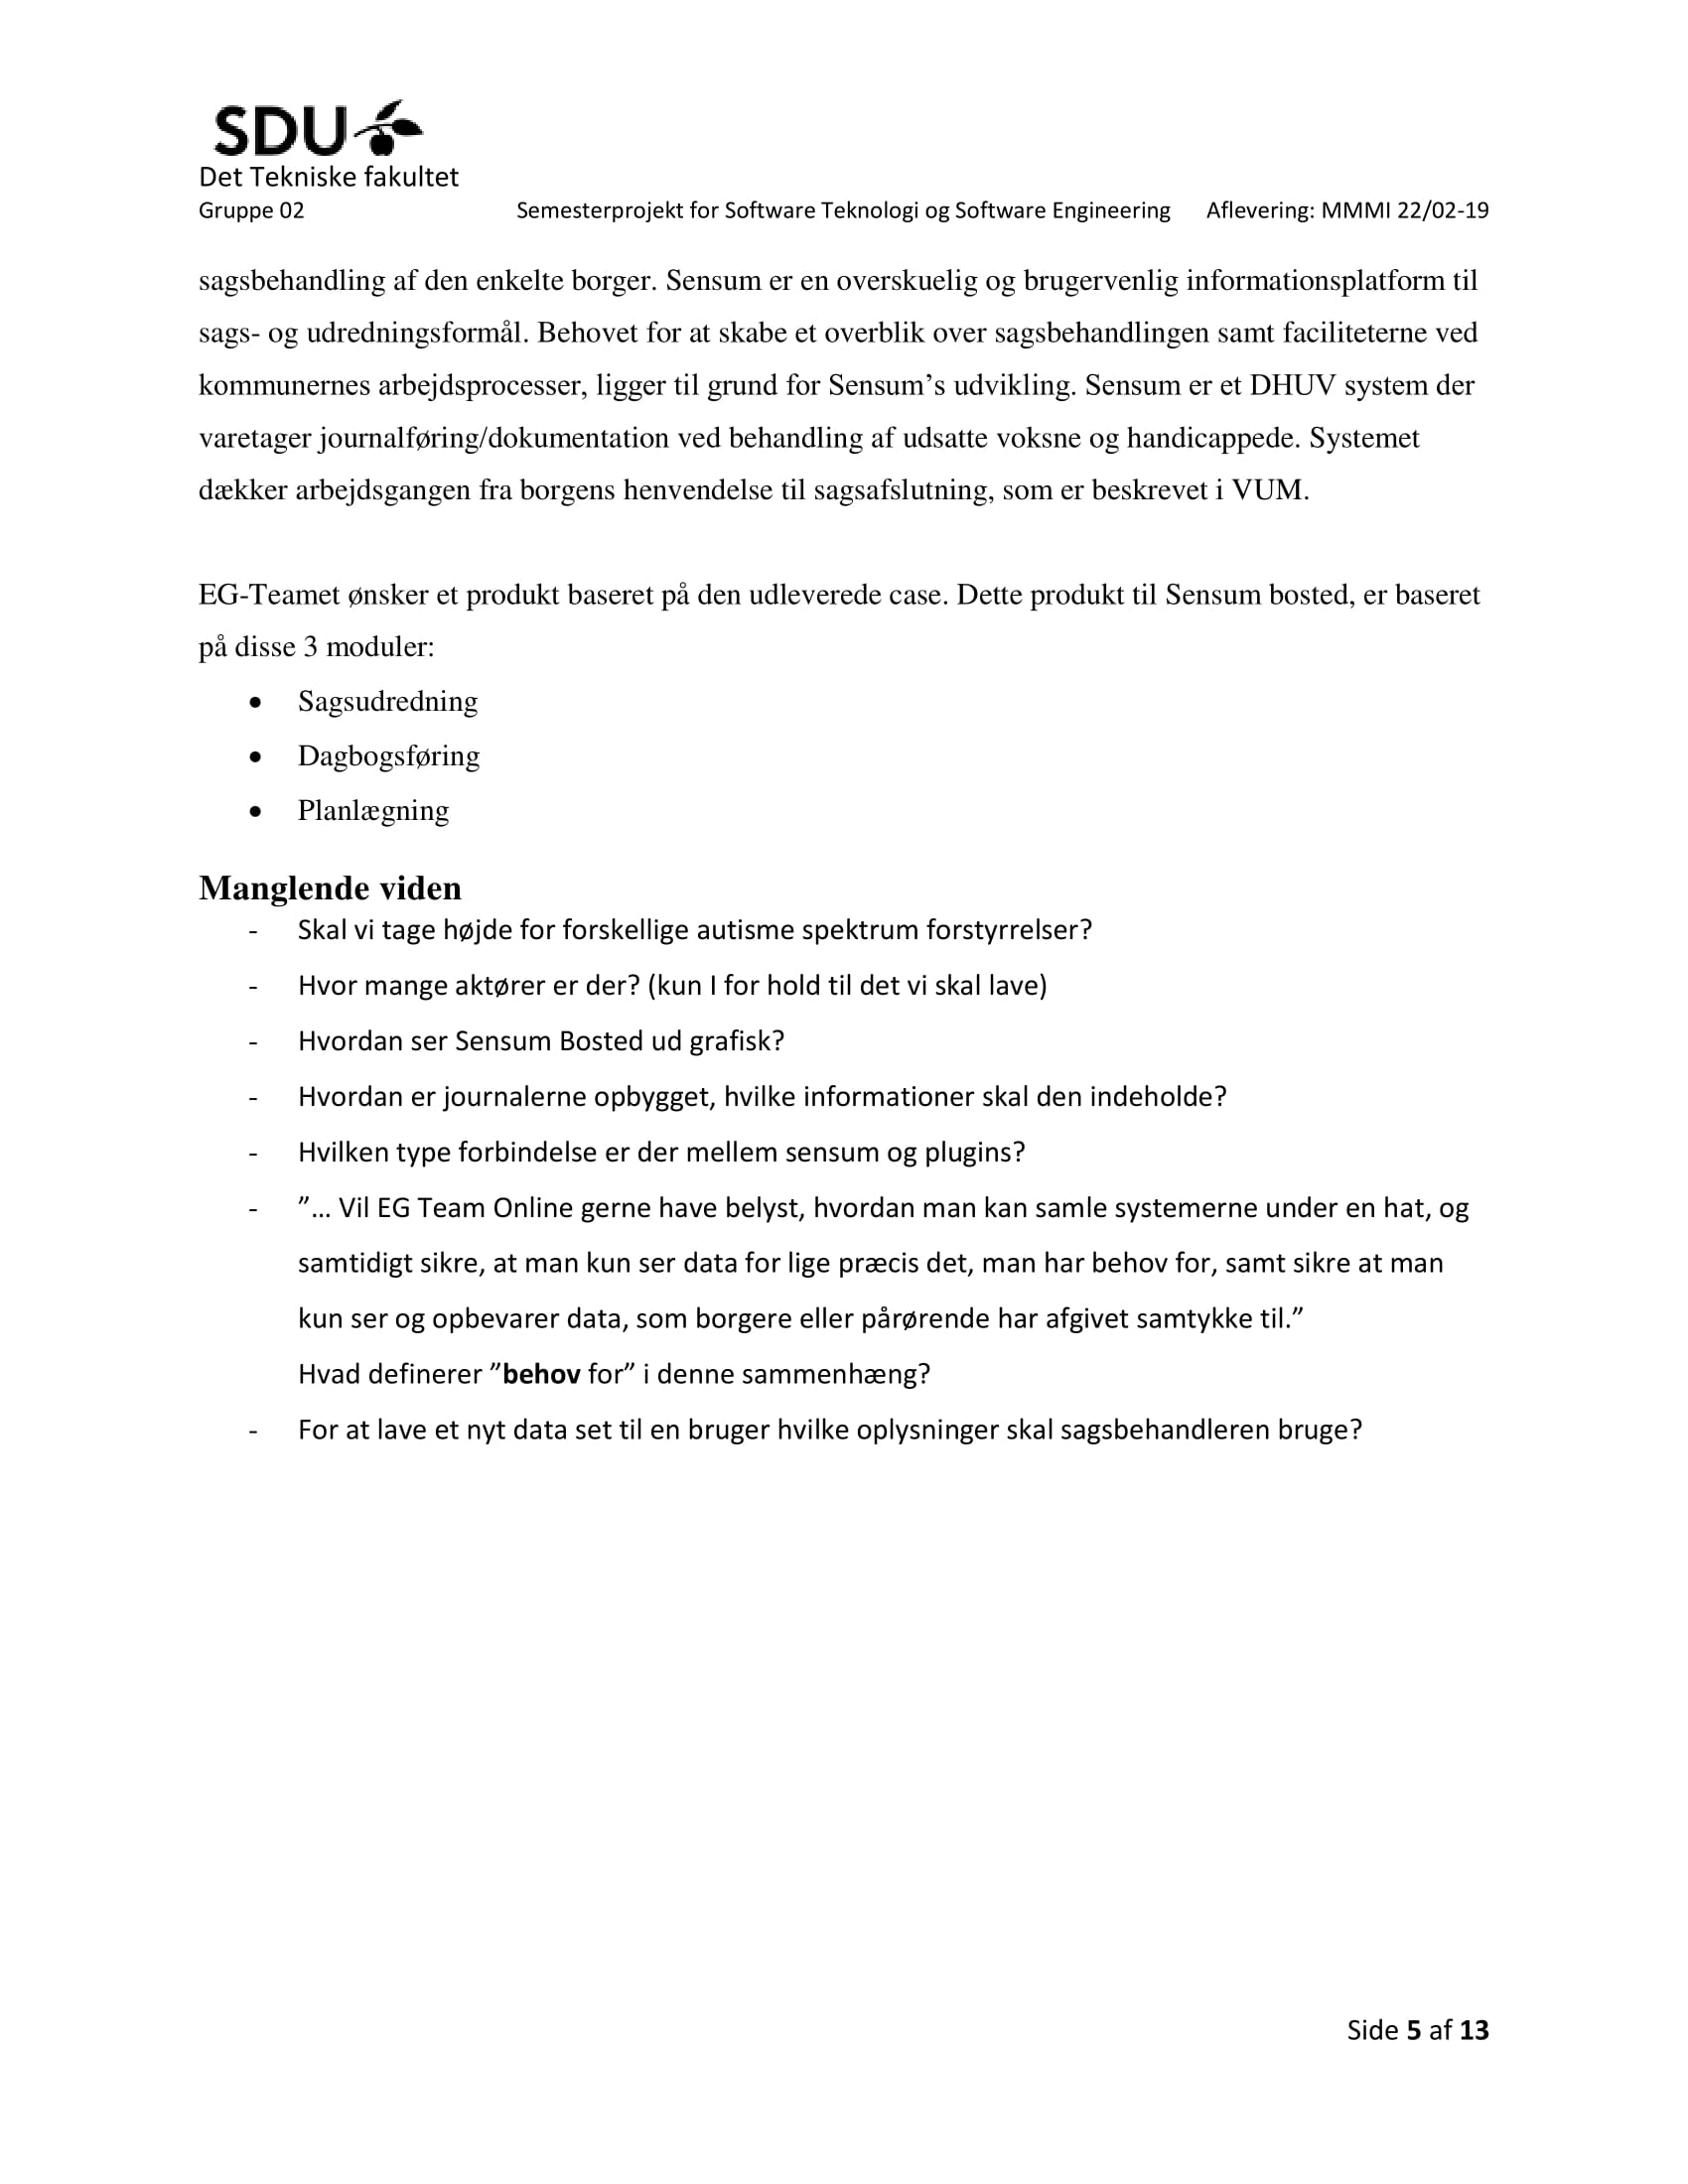
\includegraphics[scale = 0.33]{./PNG/Projektforslag/Projektforslag-05.jpg} 
\end{figure}
\begin{landscape}
\begin{figure}[hb]
  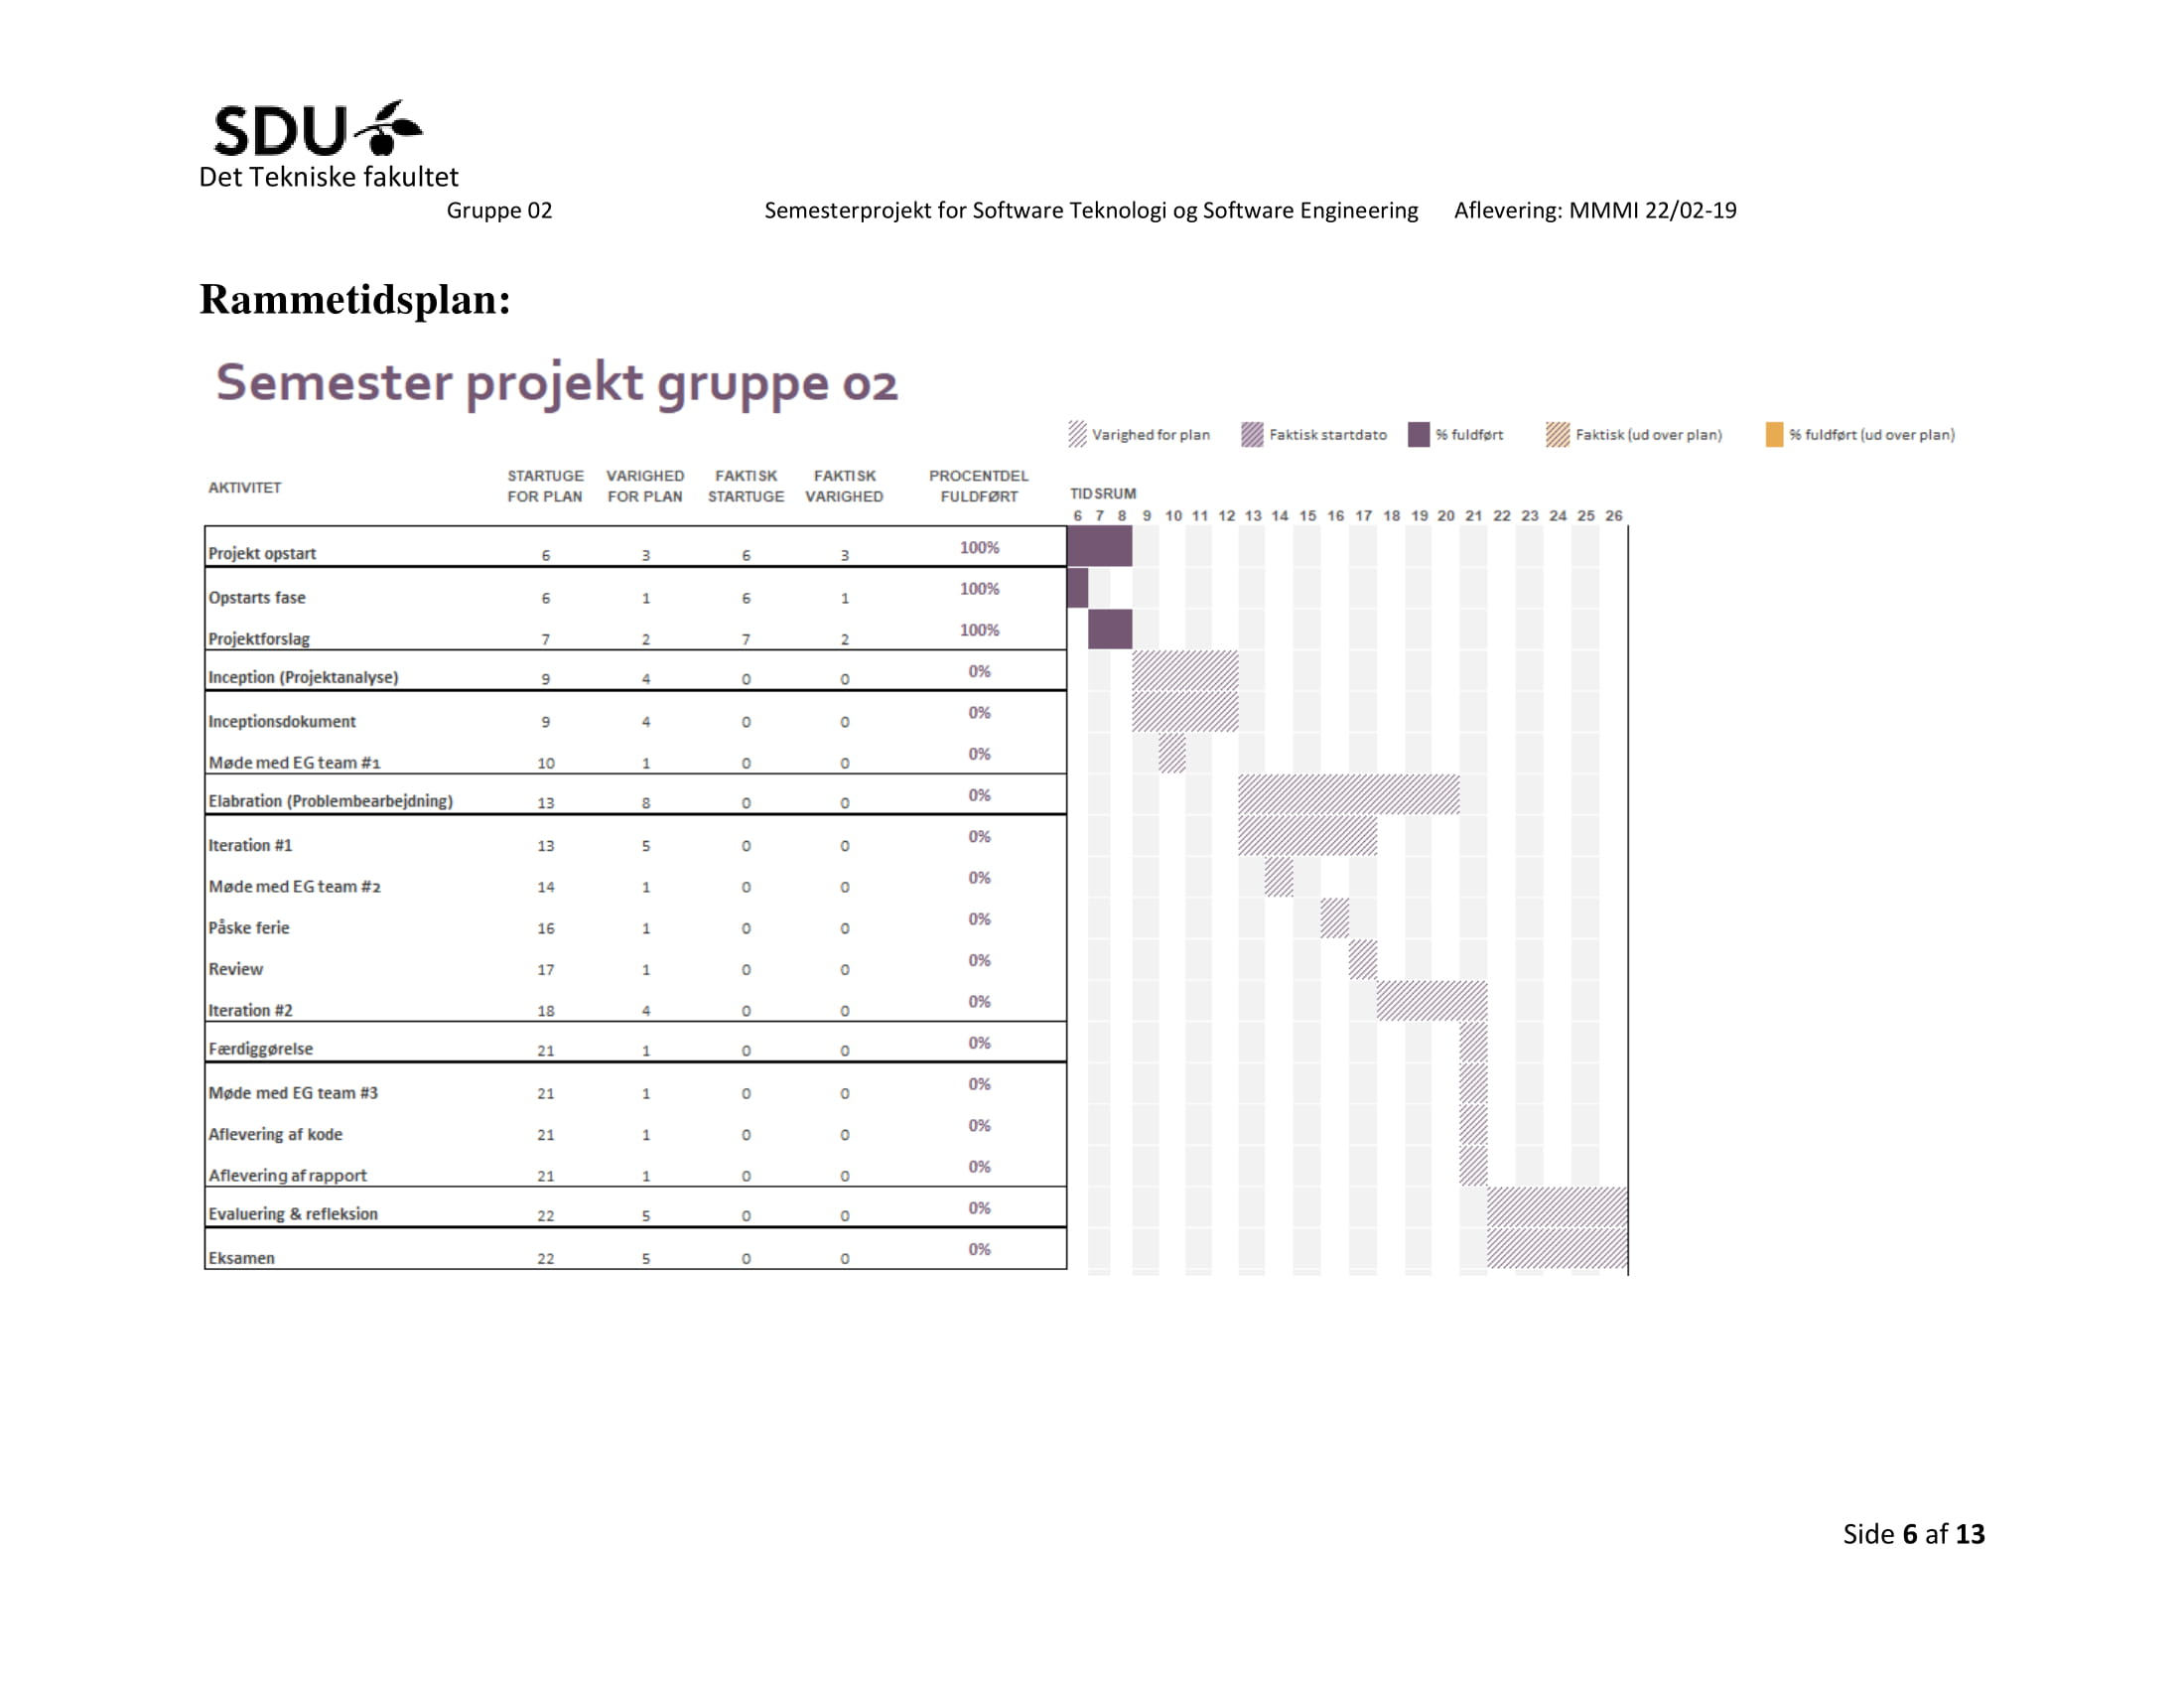
\includegraphics[scale = 0.33]{./PNG/Projektforslag/Projektforslag-06.jpg} 
\end{figure}
\end{landscape}

\begin{figure}[hb]
  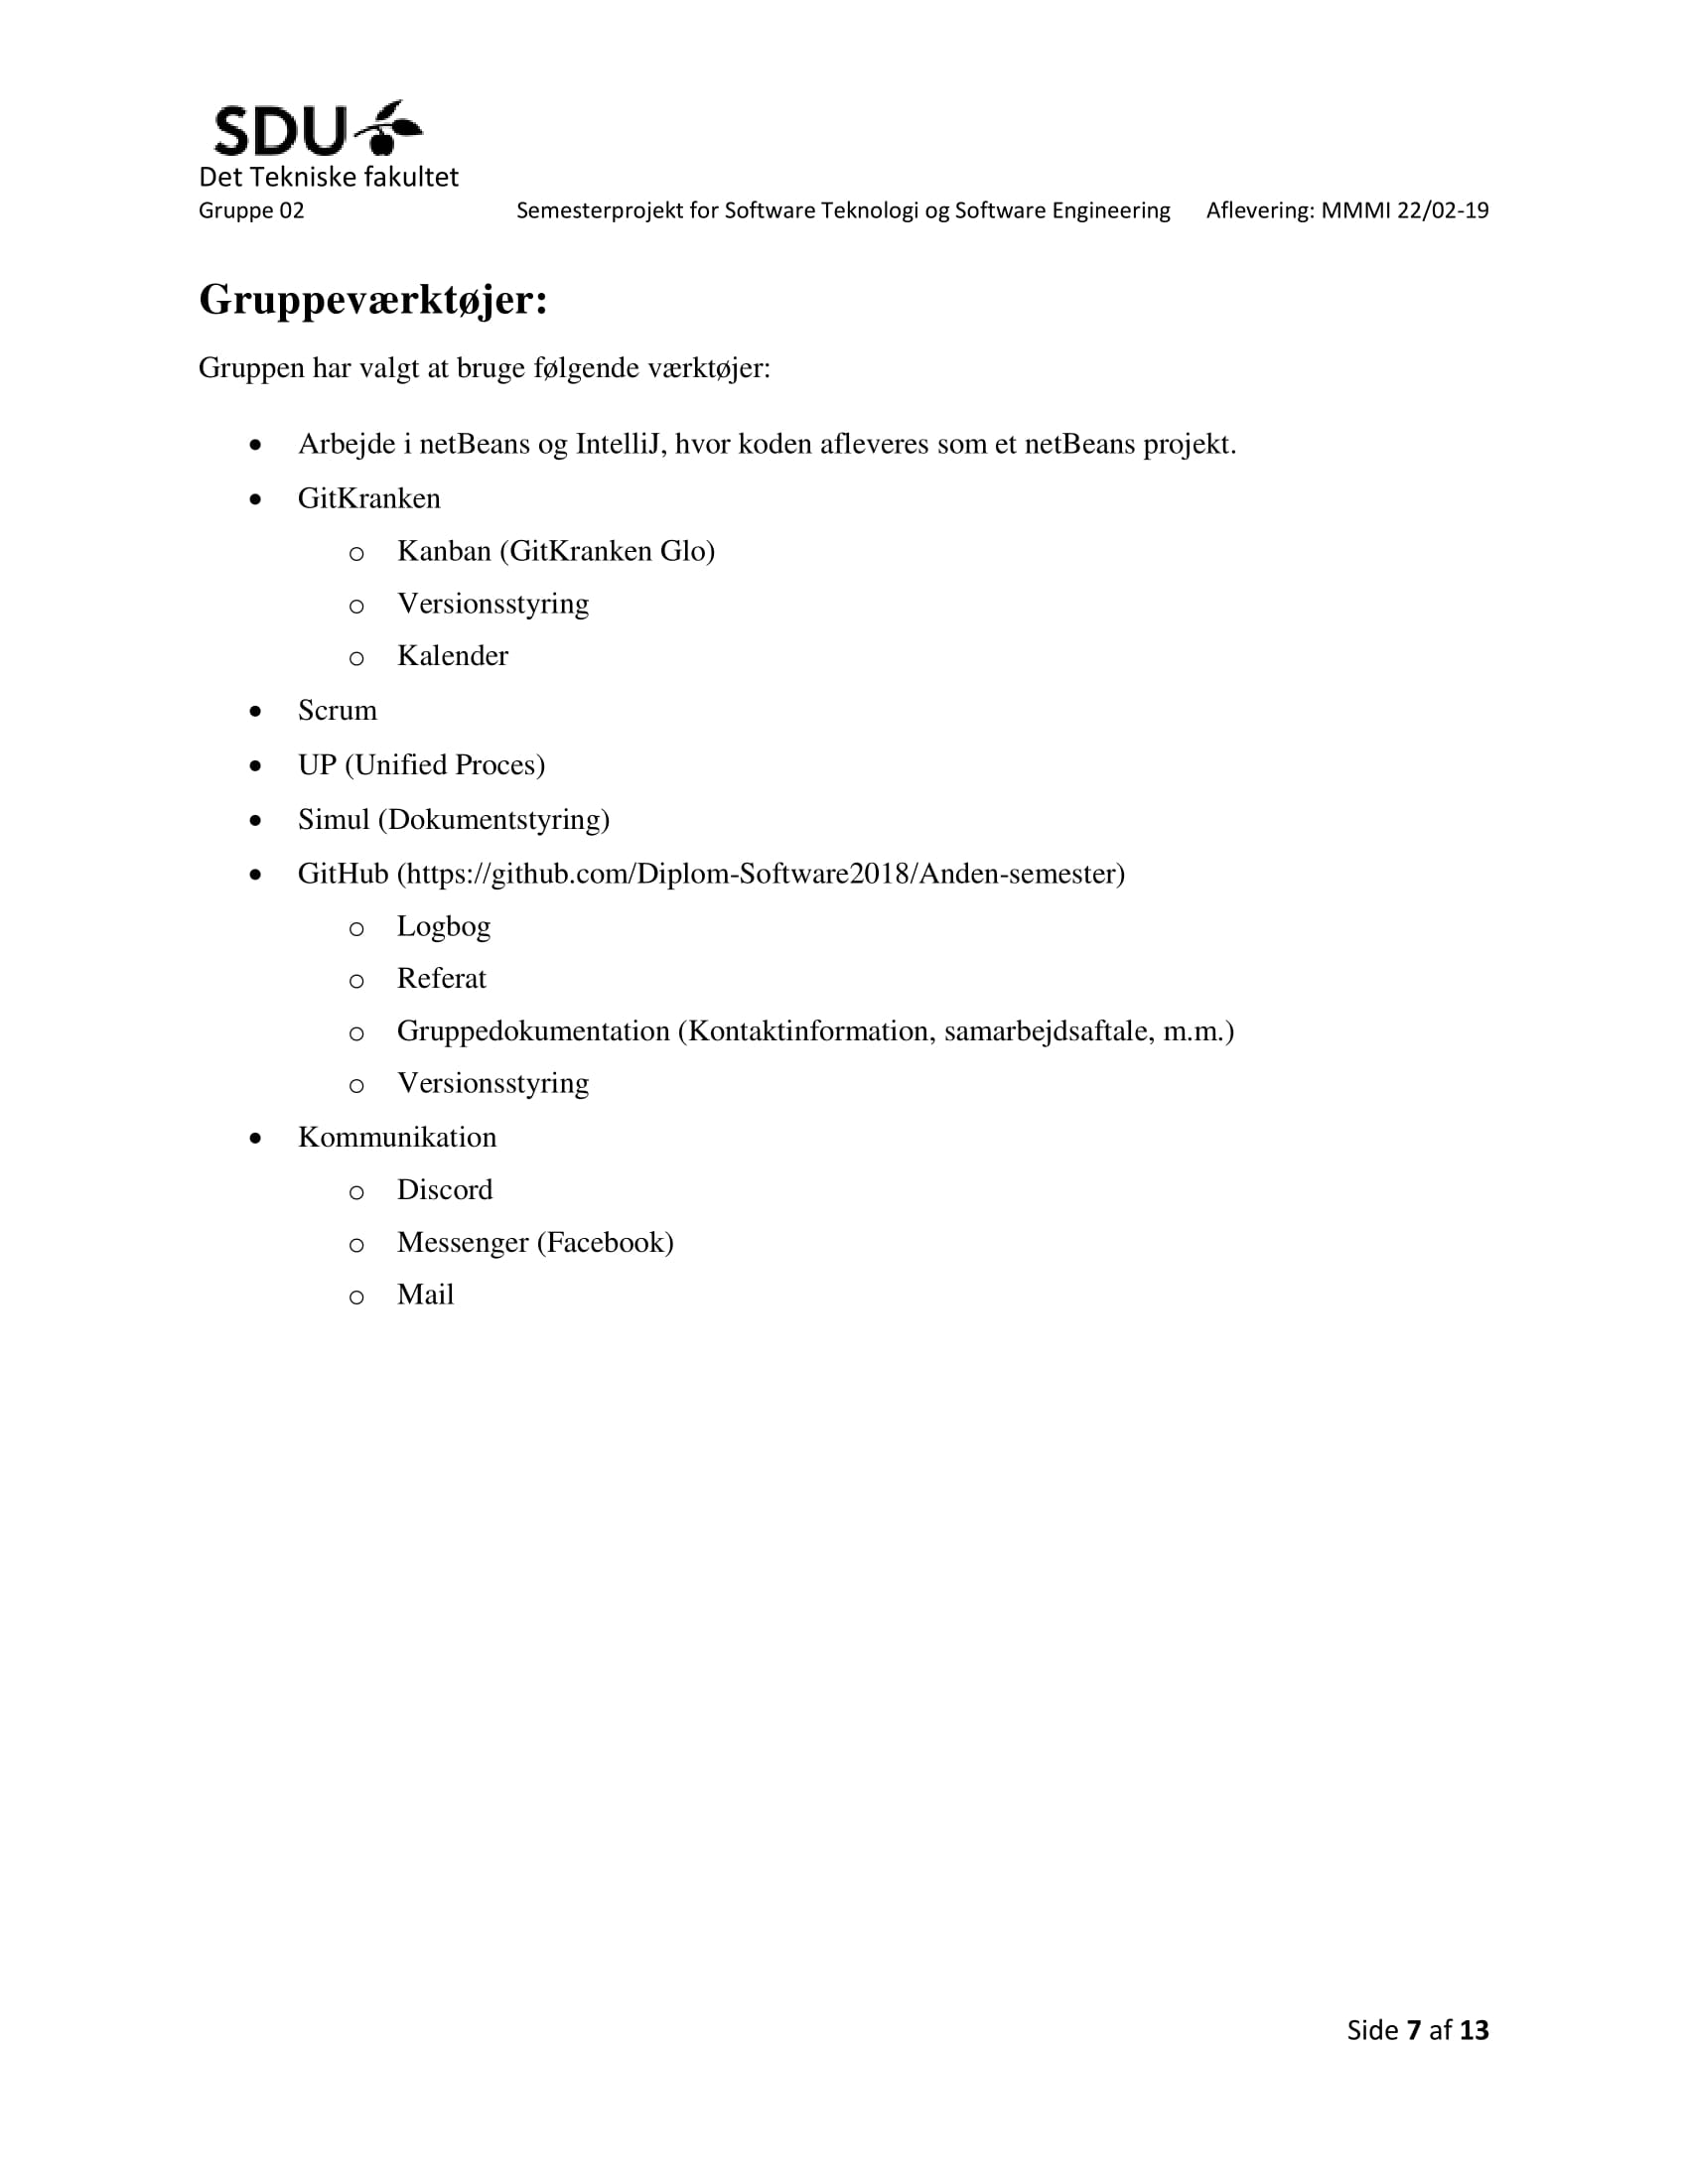
\includegraphics[scale = 0.33]{./PNG/Projektforslag/Projektforslag-07.jpg} 
\end{figure}

\begin{figure}[hb]
  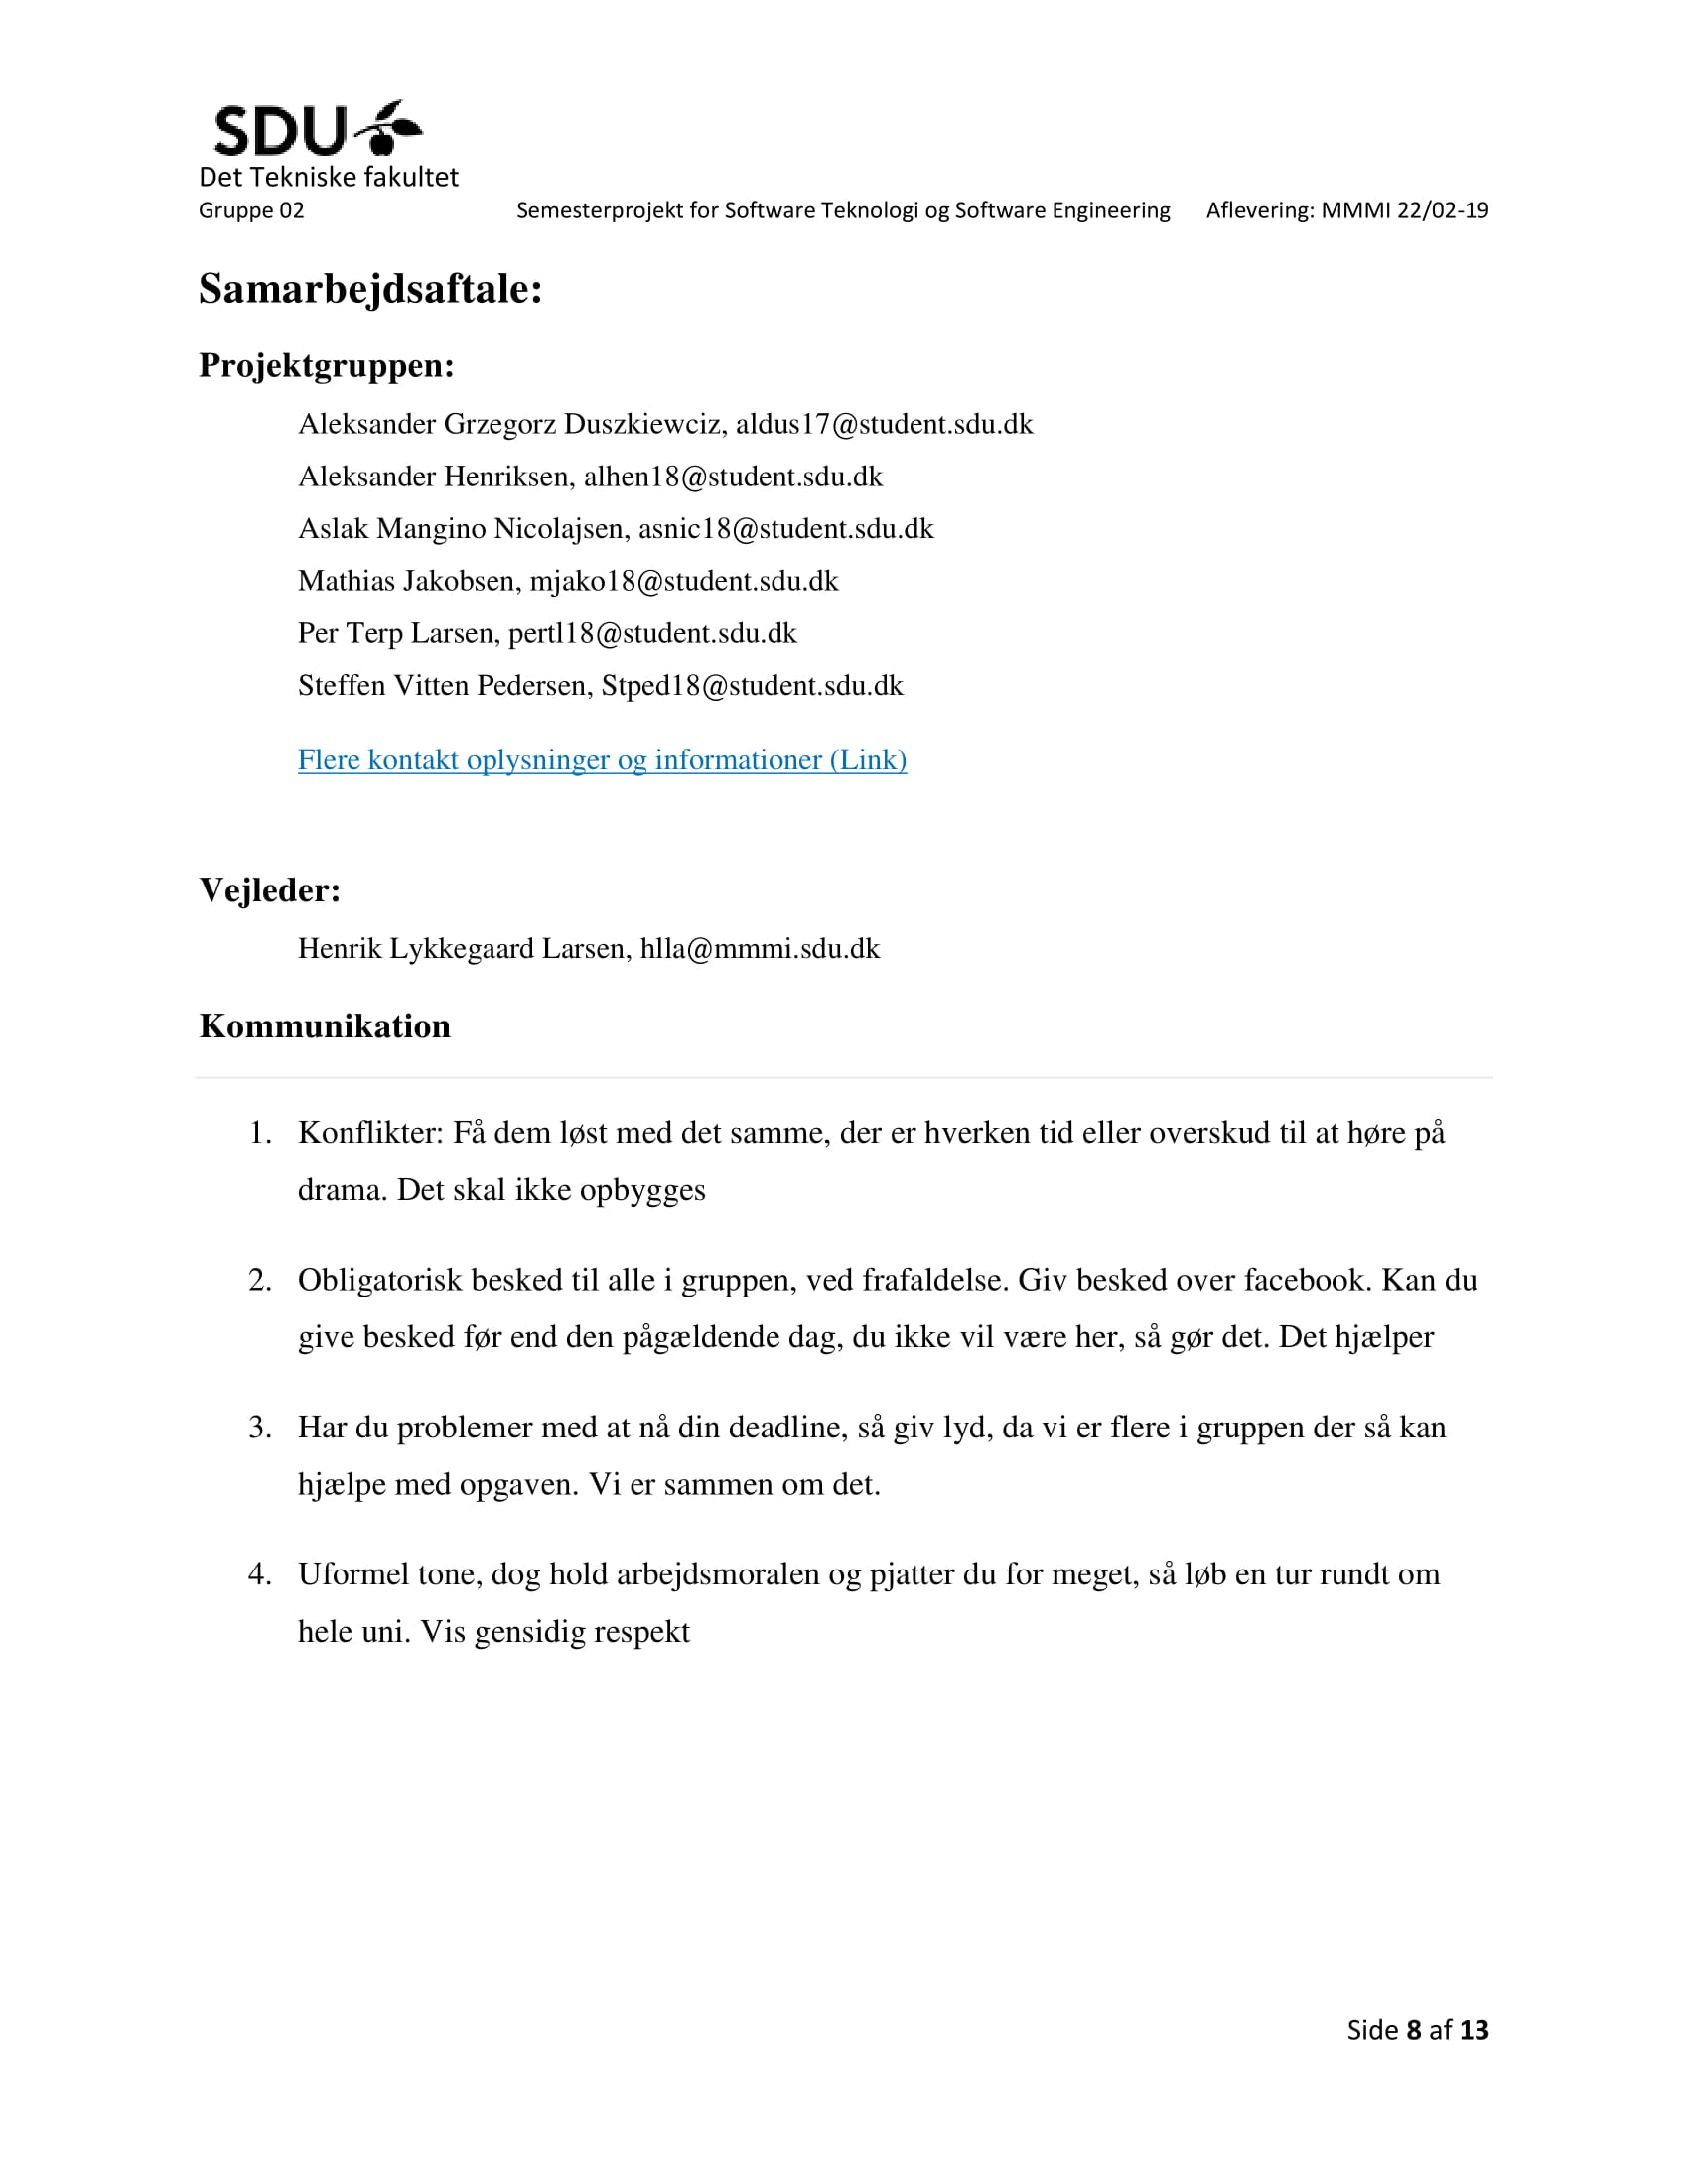
\includegraphics[scale = 0.33]{./PNG/Projektforslag/Projektforslag-08.jpg} 
\end{figure}

\begin{figure}[hb]
  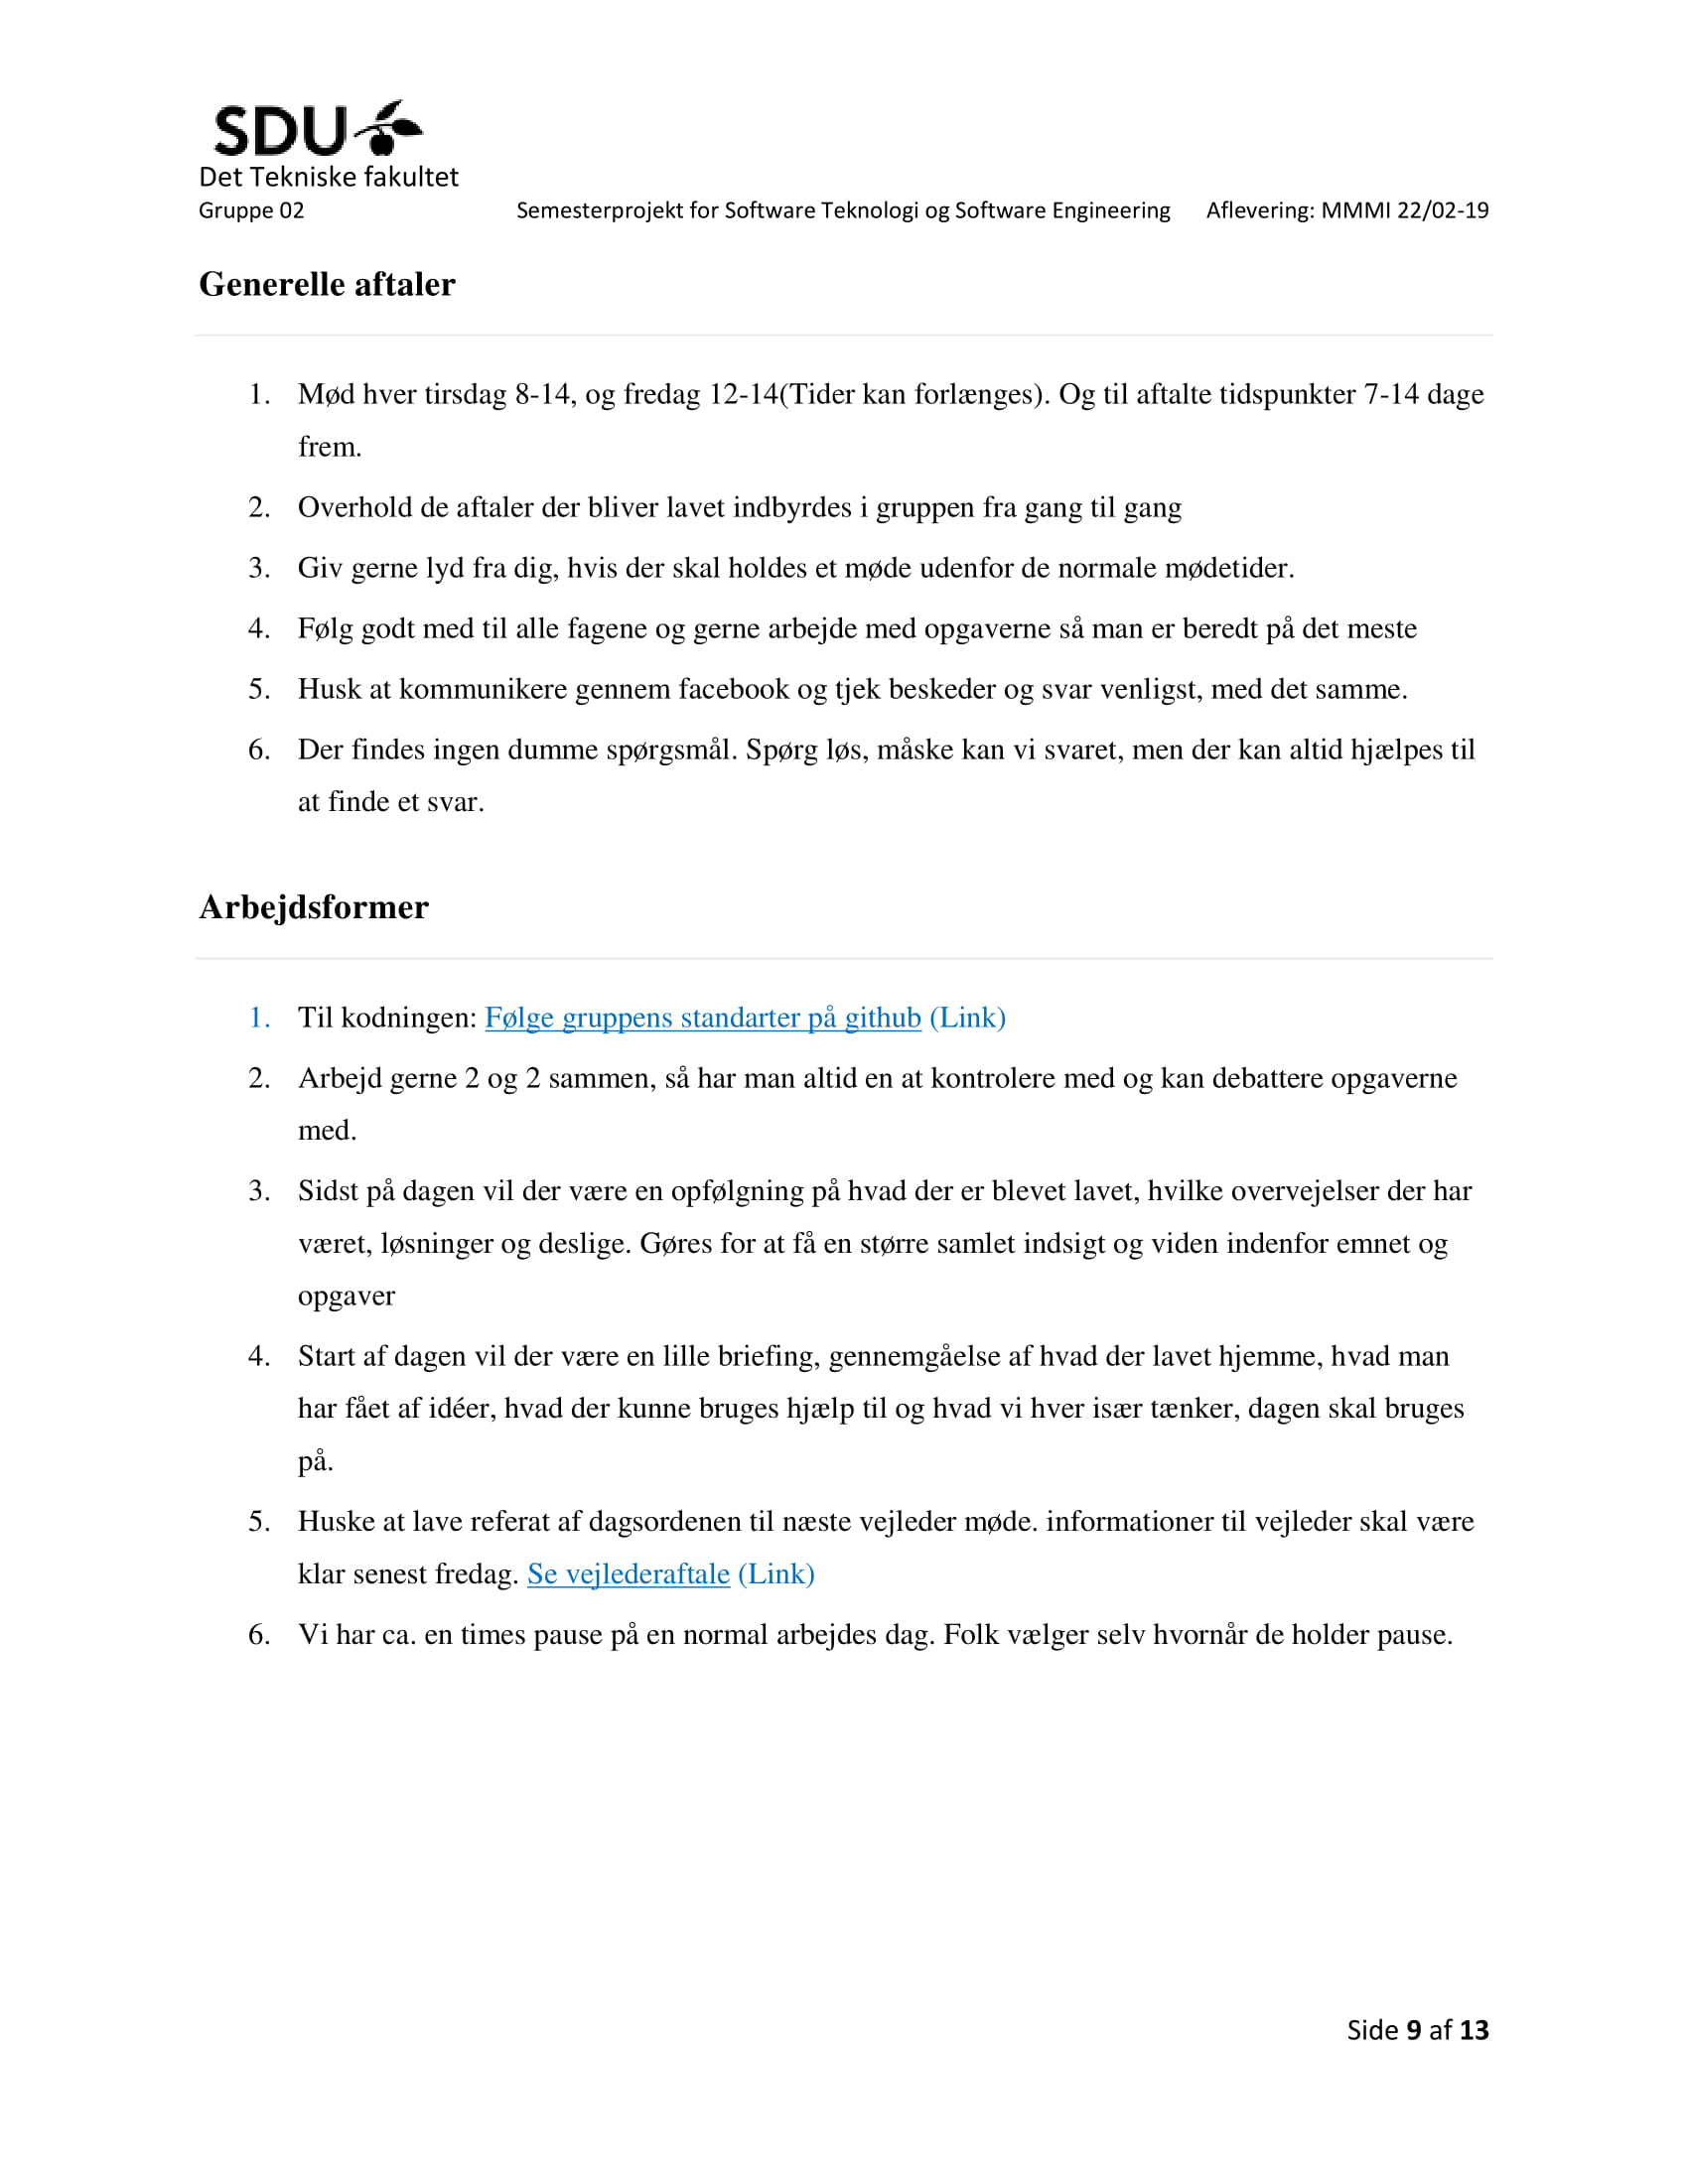
\includegraphics[scale = 0.33]{./PNG/Projektforslag/Projektforslag-09.jpg} 
\end{figure}

\begin{figure}[hb]
  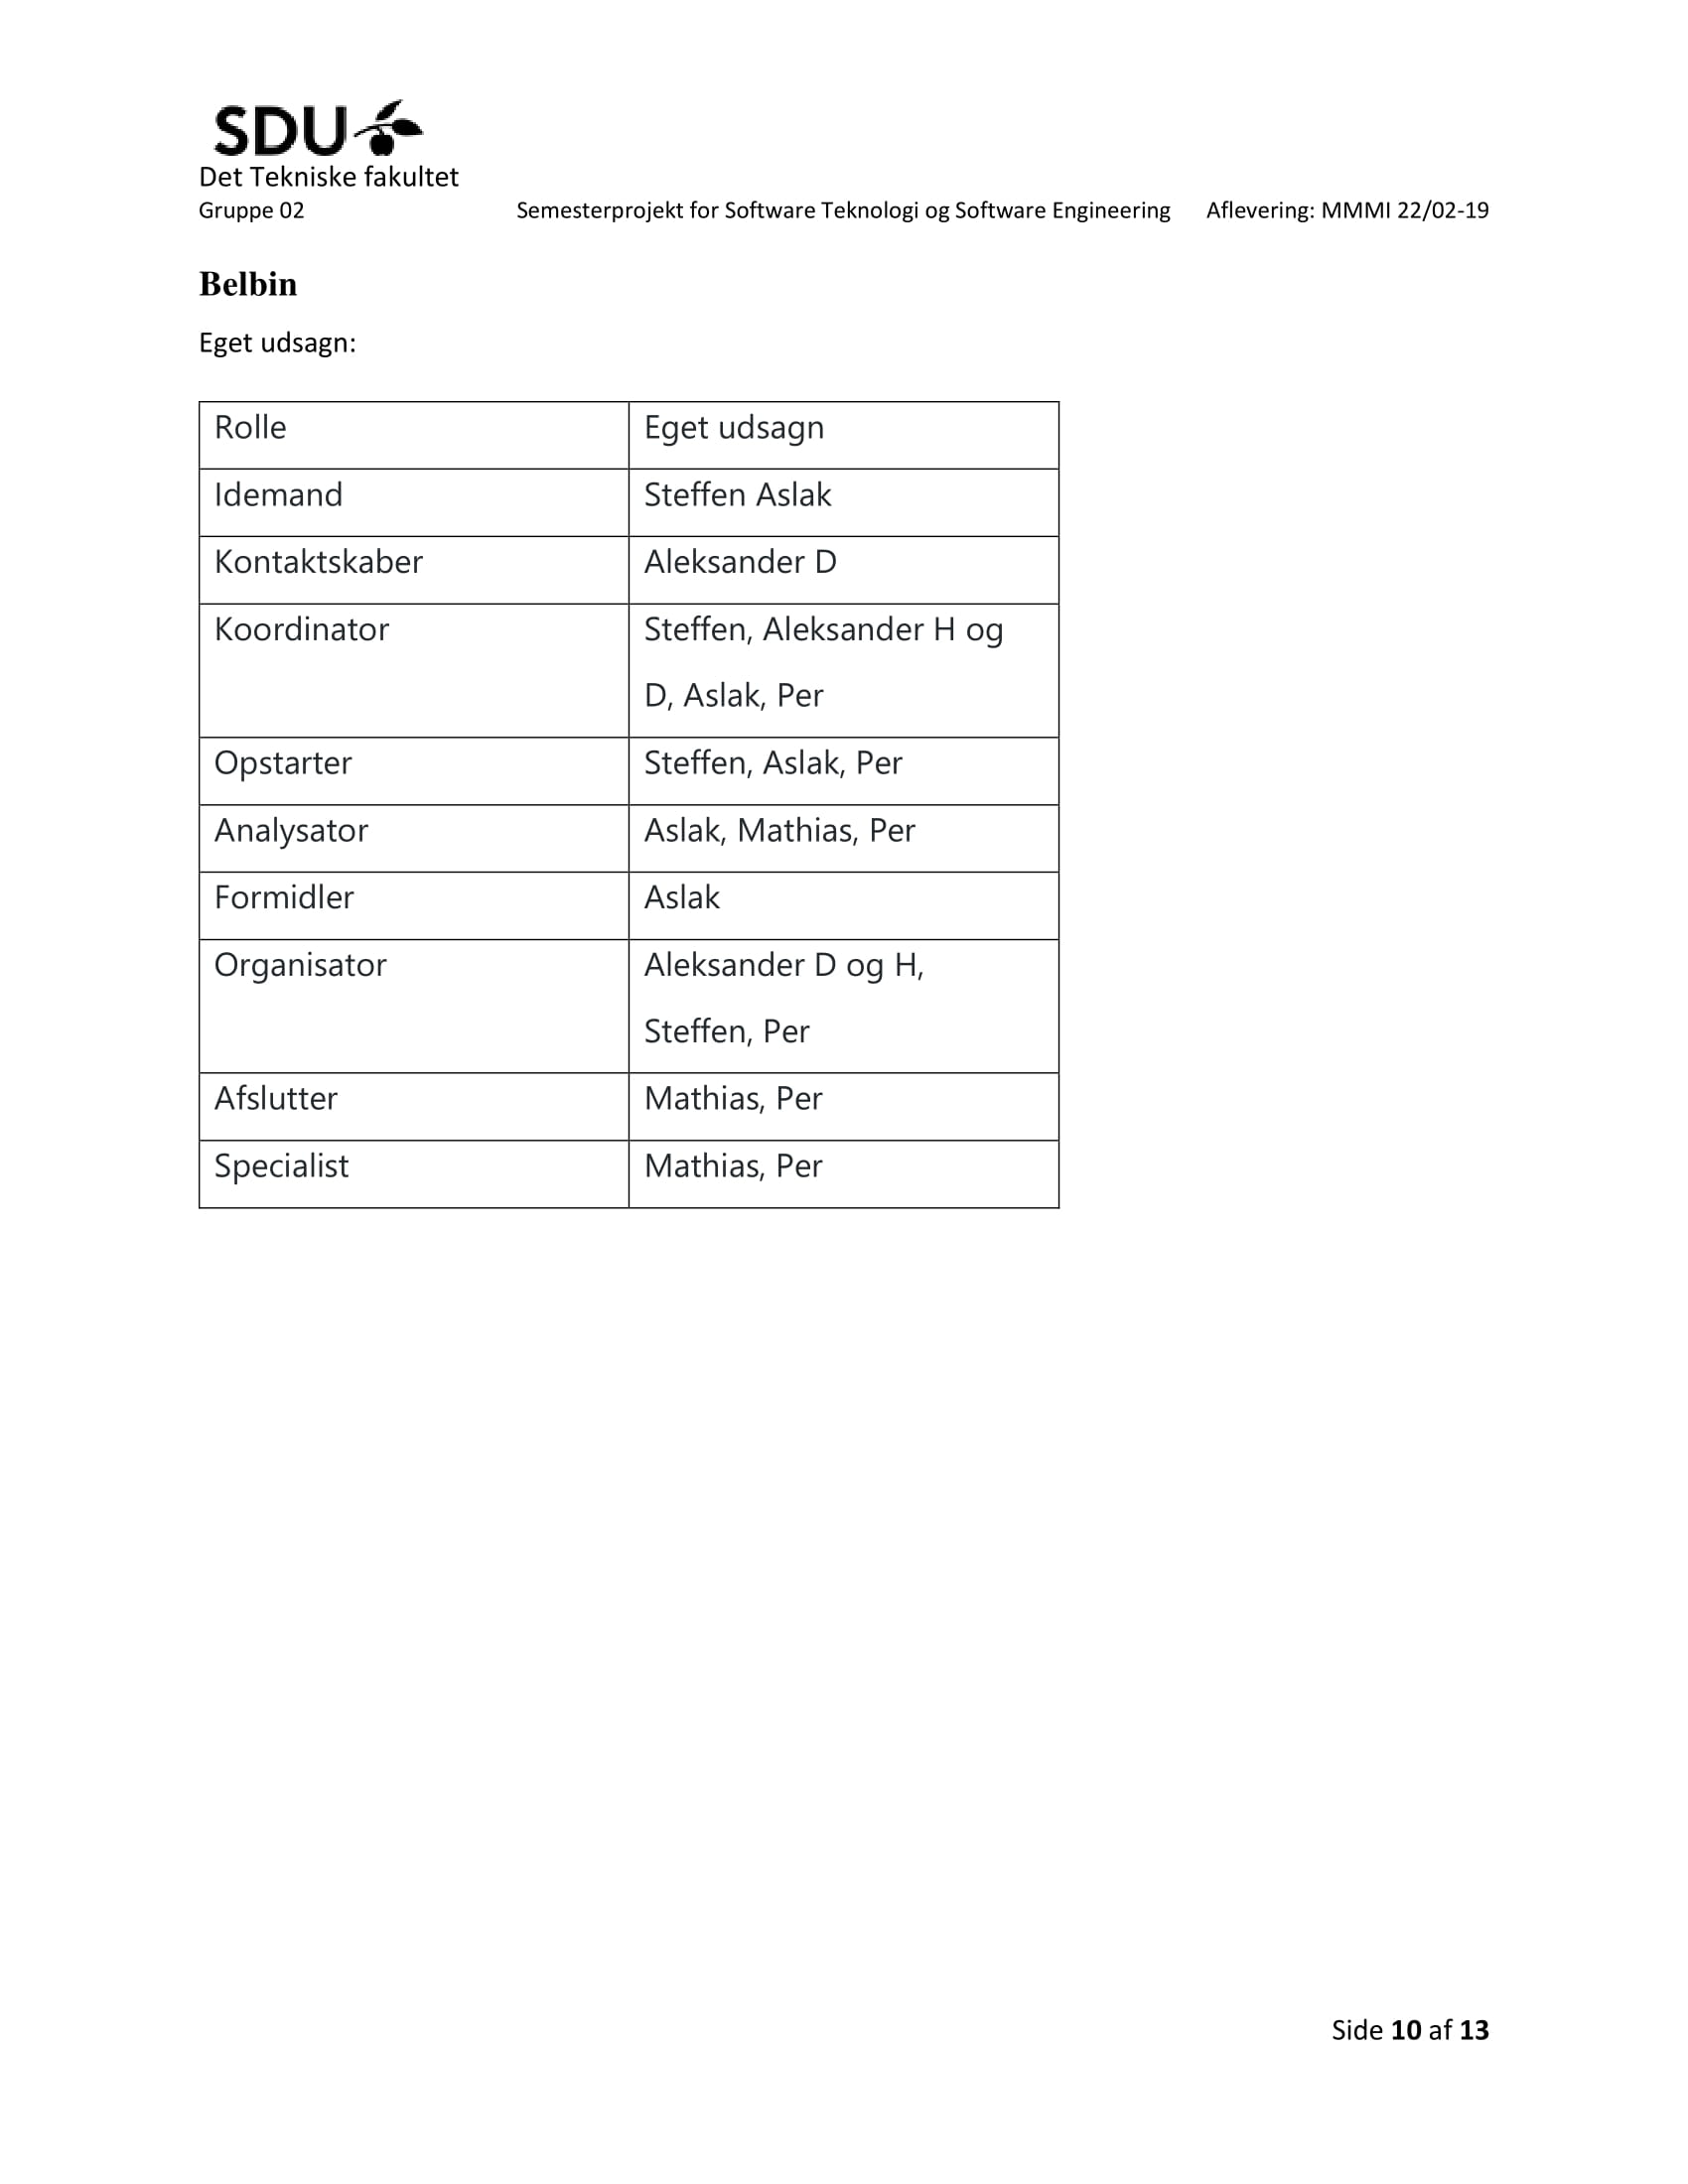
\includegraphics[scale = 0.33]{./PNG/Projektforslag/Projektforslag-10.jpg} 
\end{figure}

\begin{figure}[hb]
  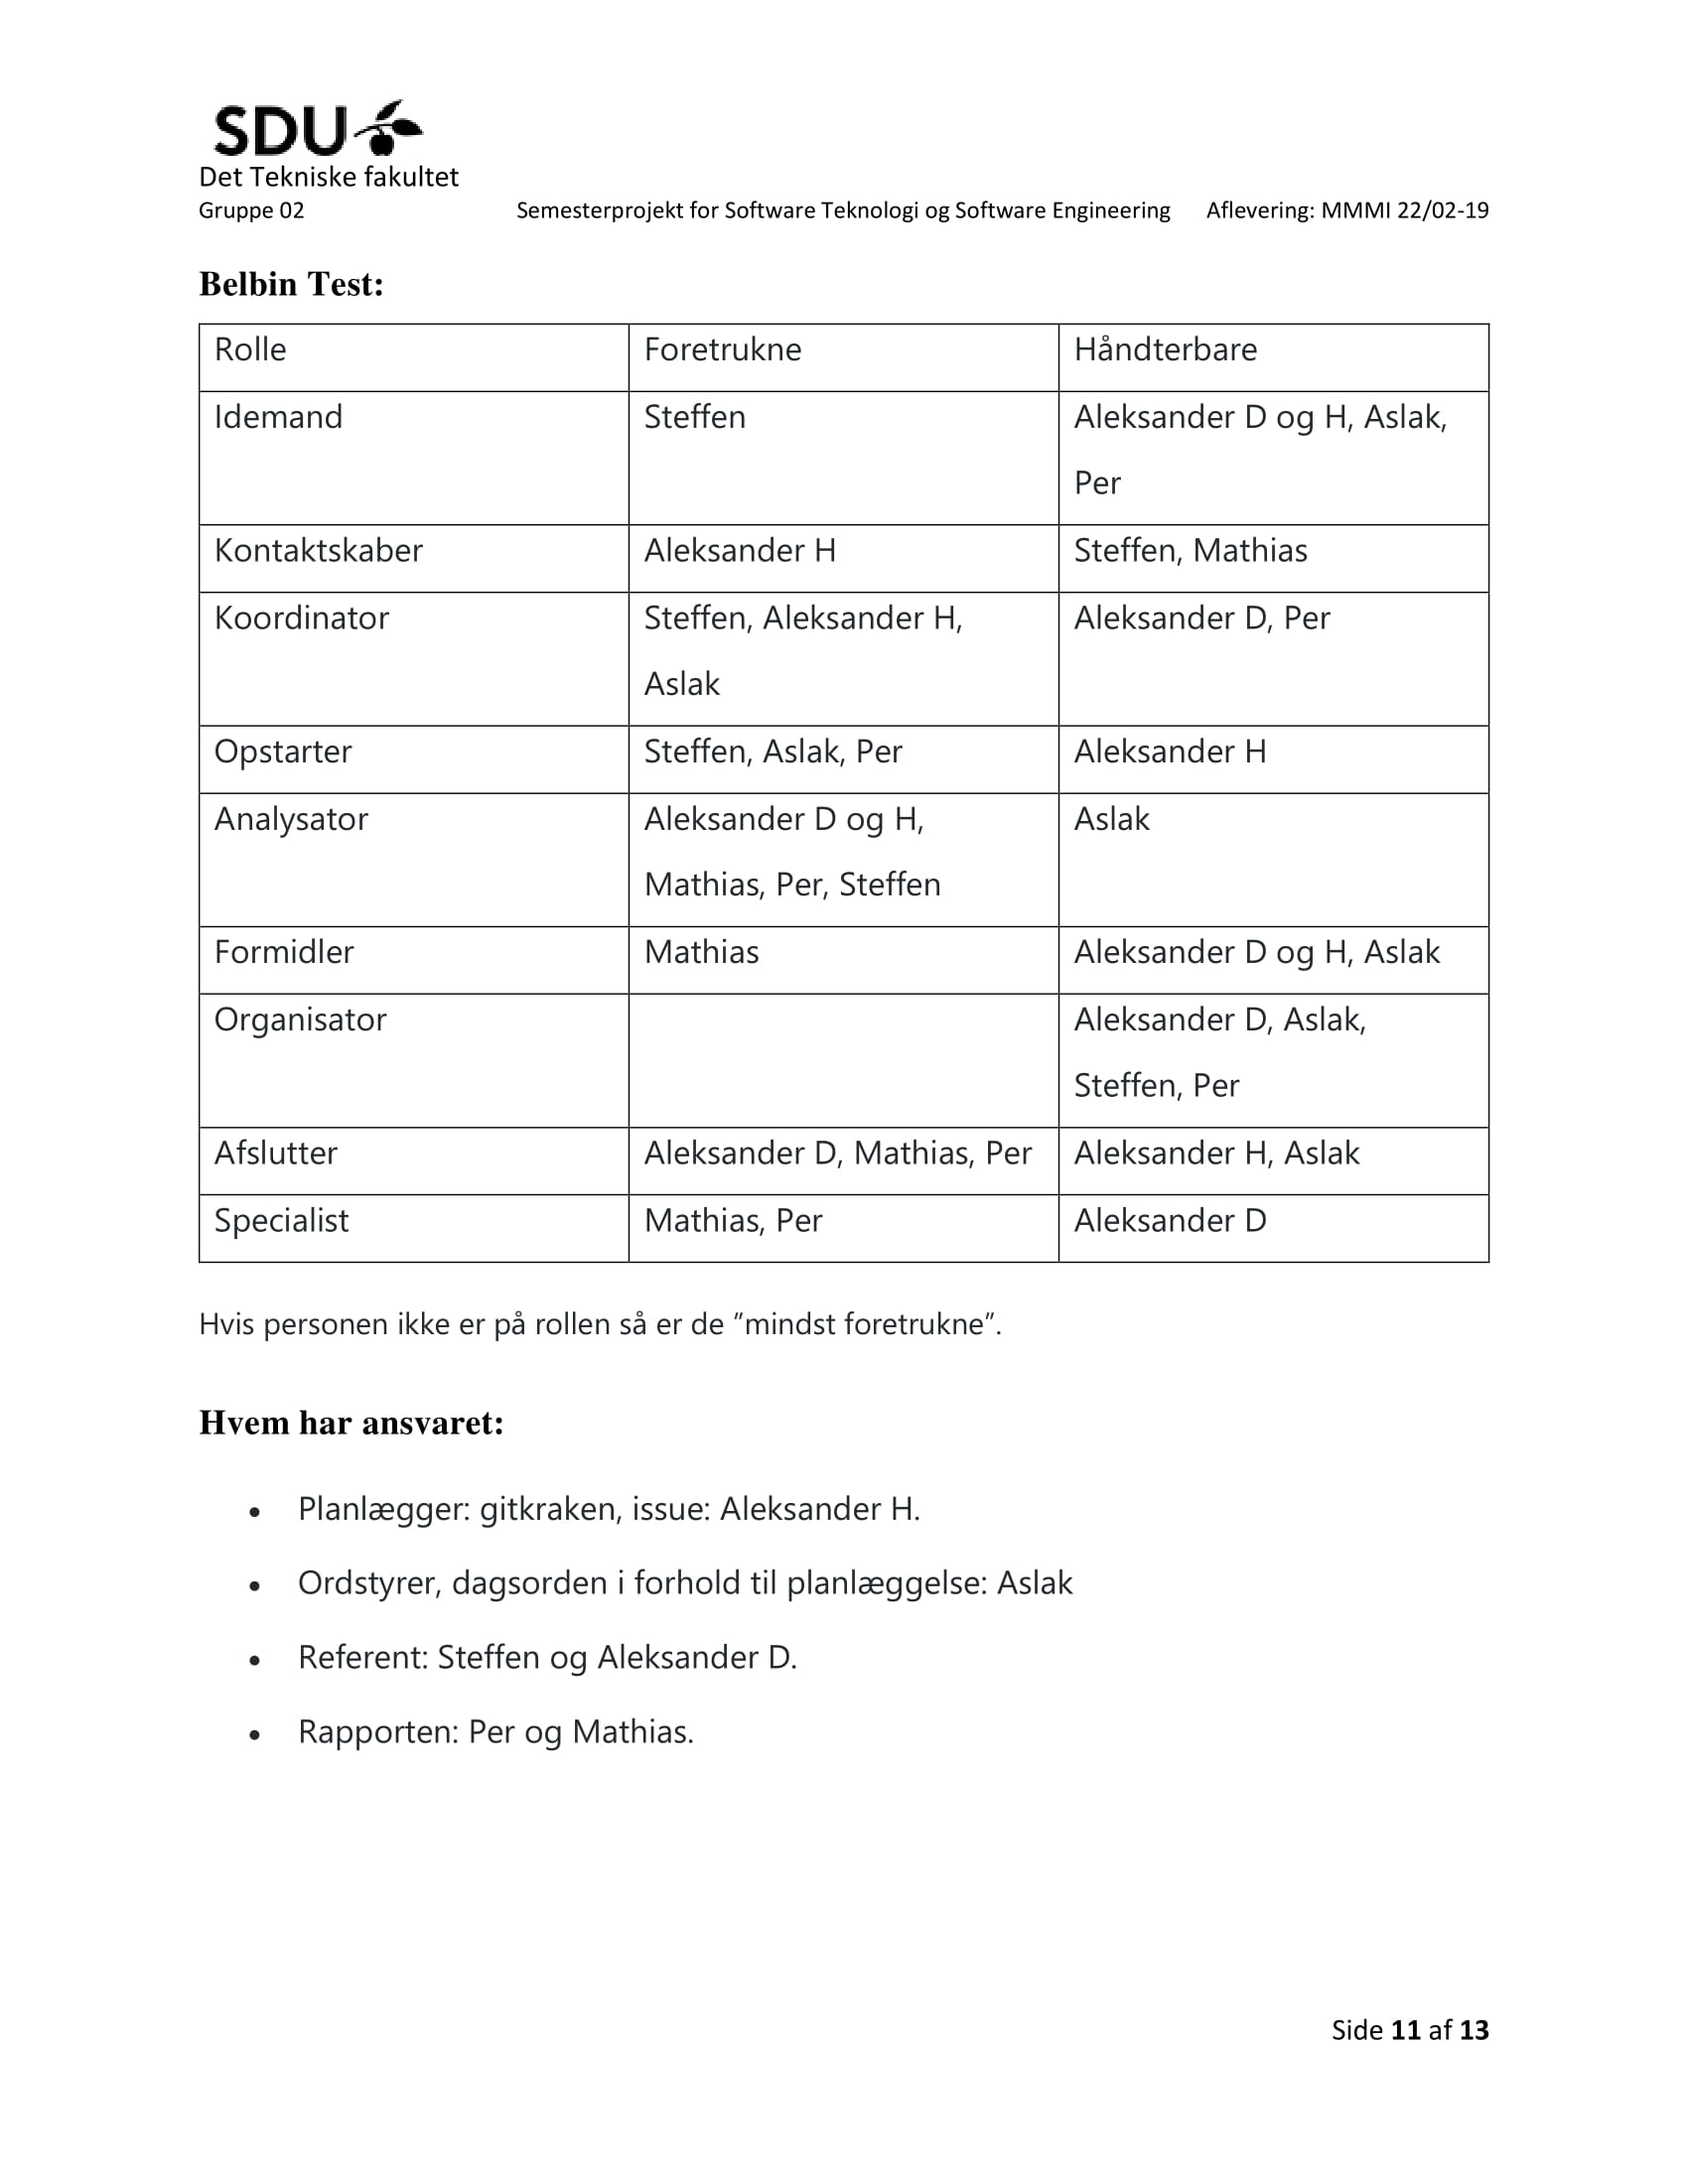
\includegraphics[scale = 0.33]{./PNG/Projektforslag/Projektforslag-11.jpg} 
\end{figure}

\begin{figure}[hb]
  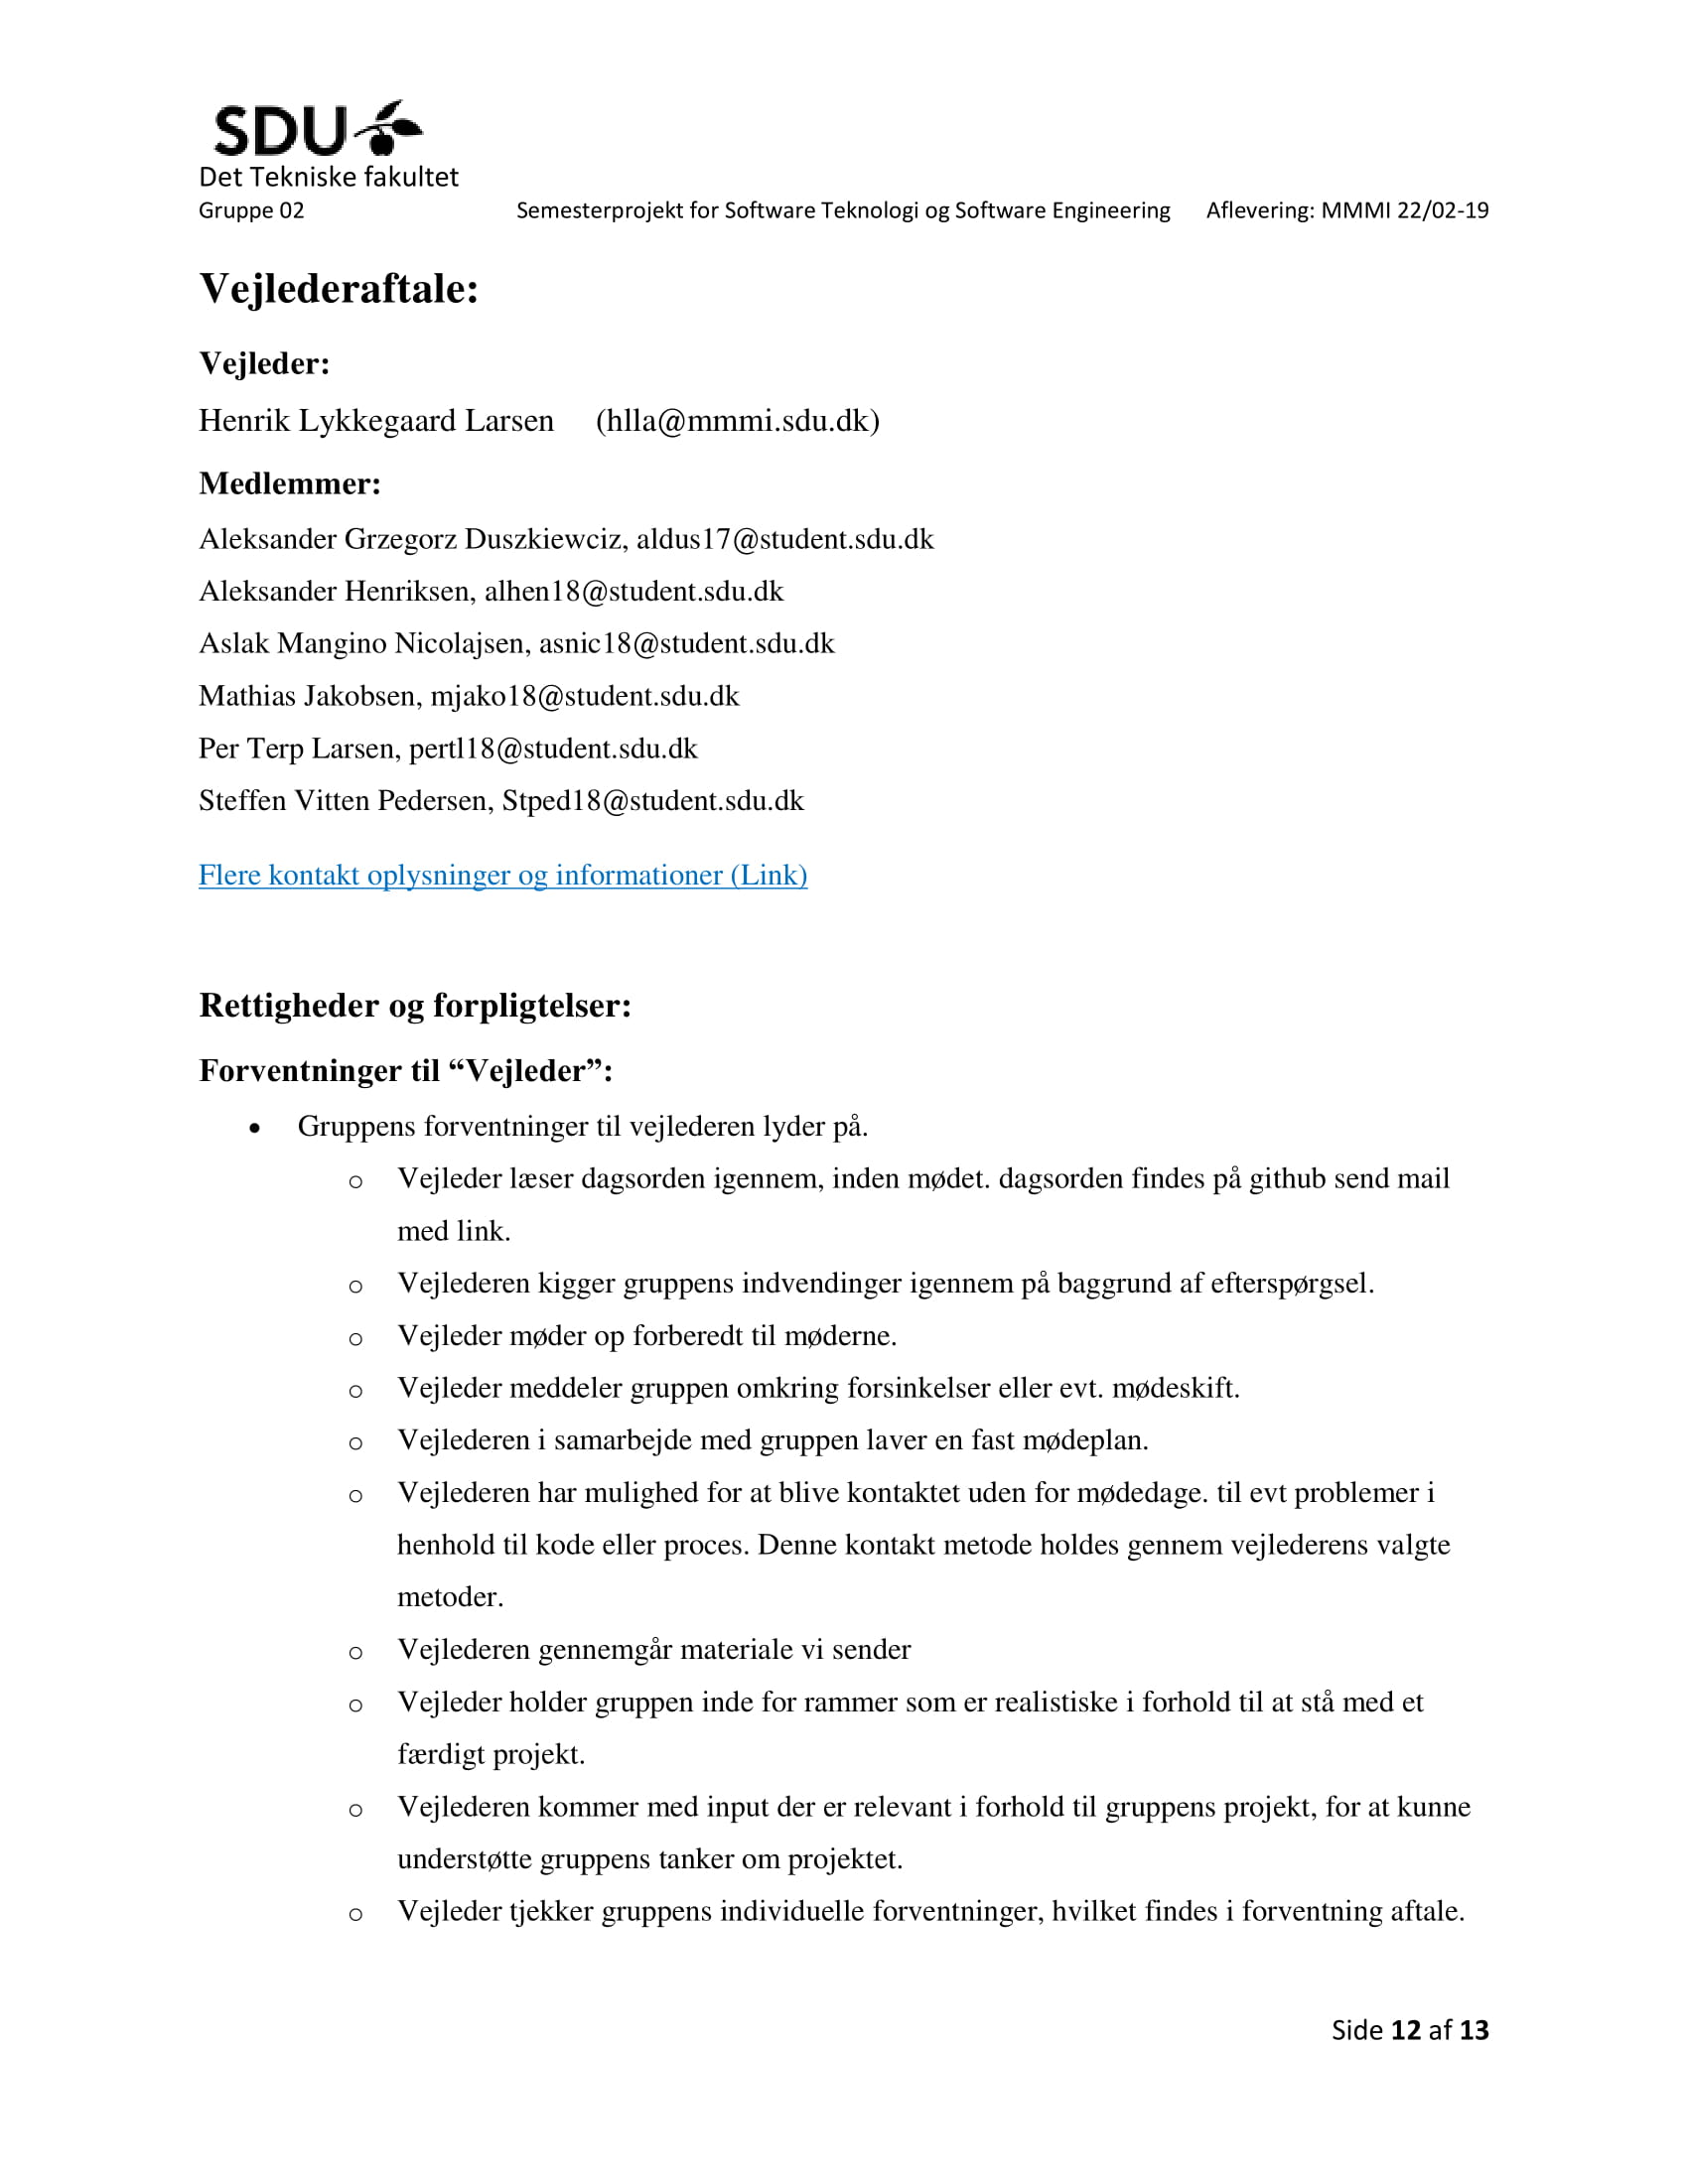
\includegraphics[scale = 0.33]{./PNG/Projektforslag/Projektforslag-12.jpg} 
\end{figure}

\begin{figure}[hb]
  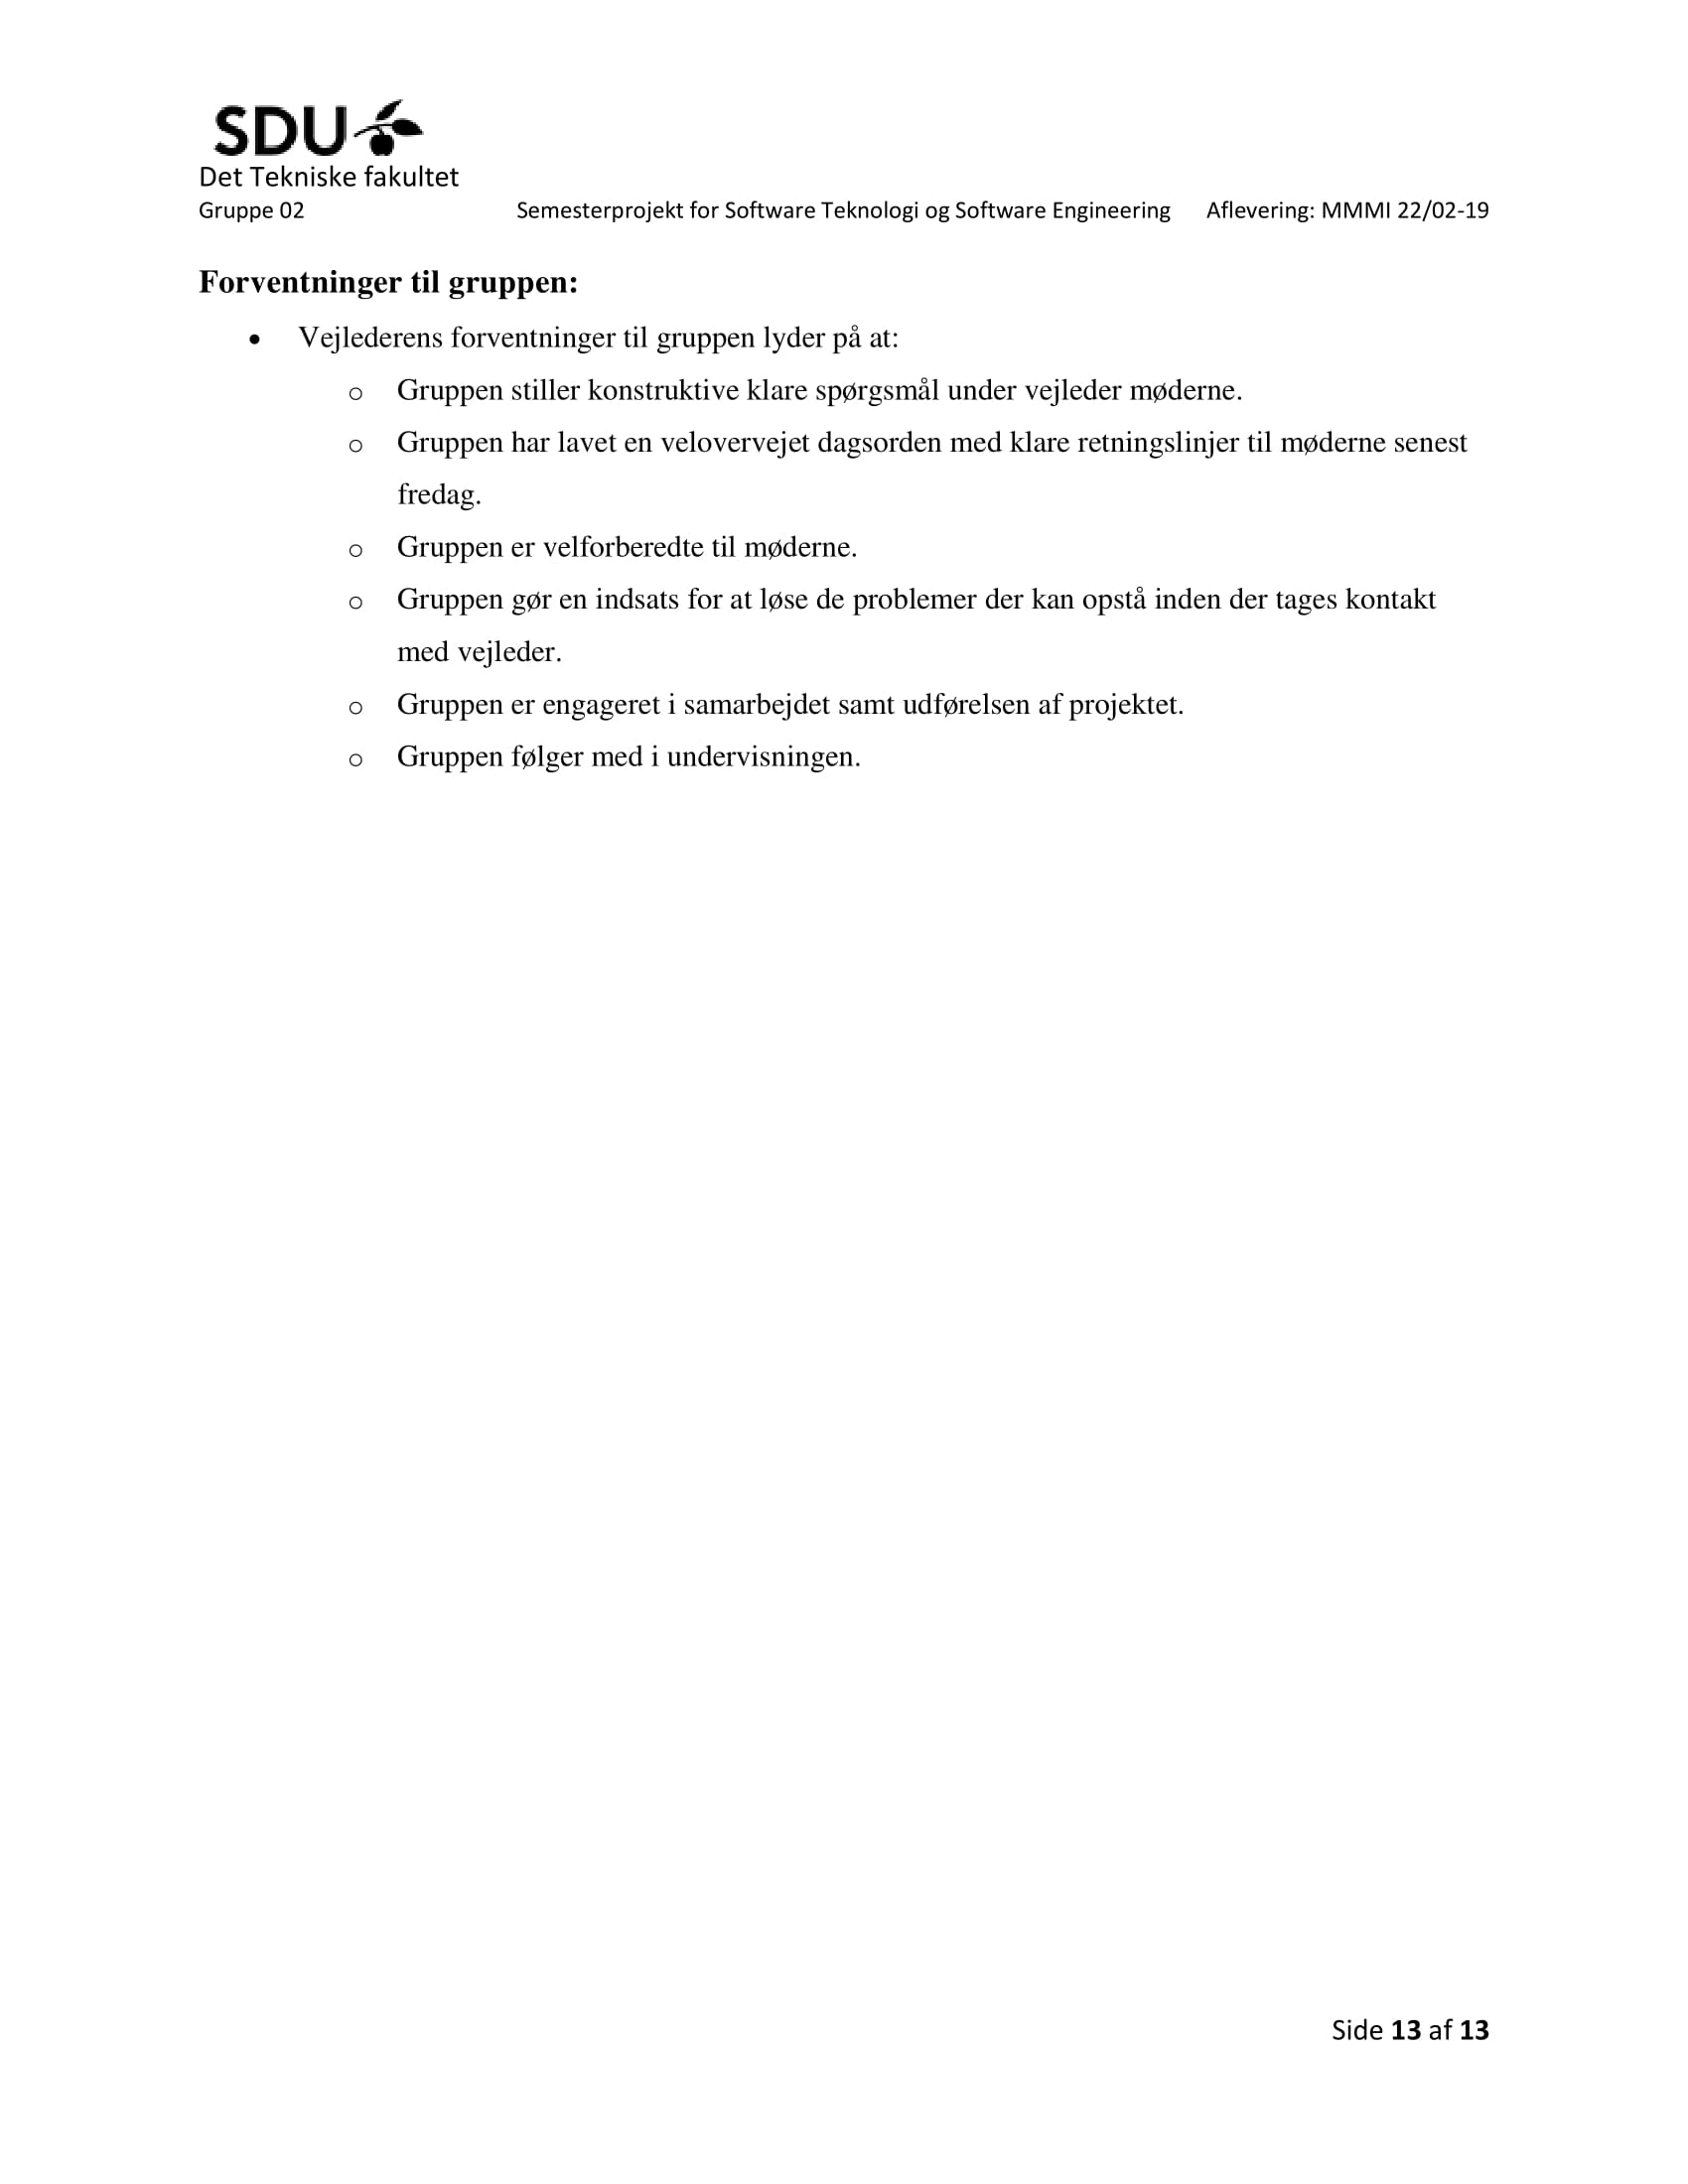
\includegraphics[scale = 0.33]{./PNG/Projektforslag/Projektforslag-13.jpg} 
\end{figure}

\section{Inceptionsdokument}

\begin{figure}[hb]
\begin{center}
  
\includegraphics[scale = 0.33]{./PNG/Inceptions/Gruppe 02 + InceptionsDokument-01.jpg} 
\end{center}
\end{figure}

\begin{figure}[hb]
  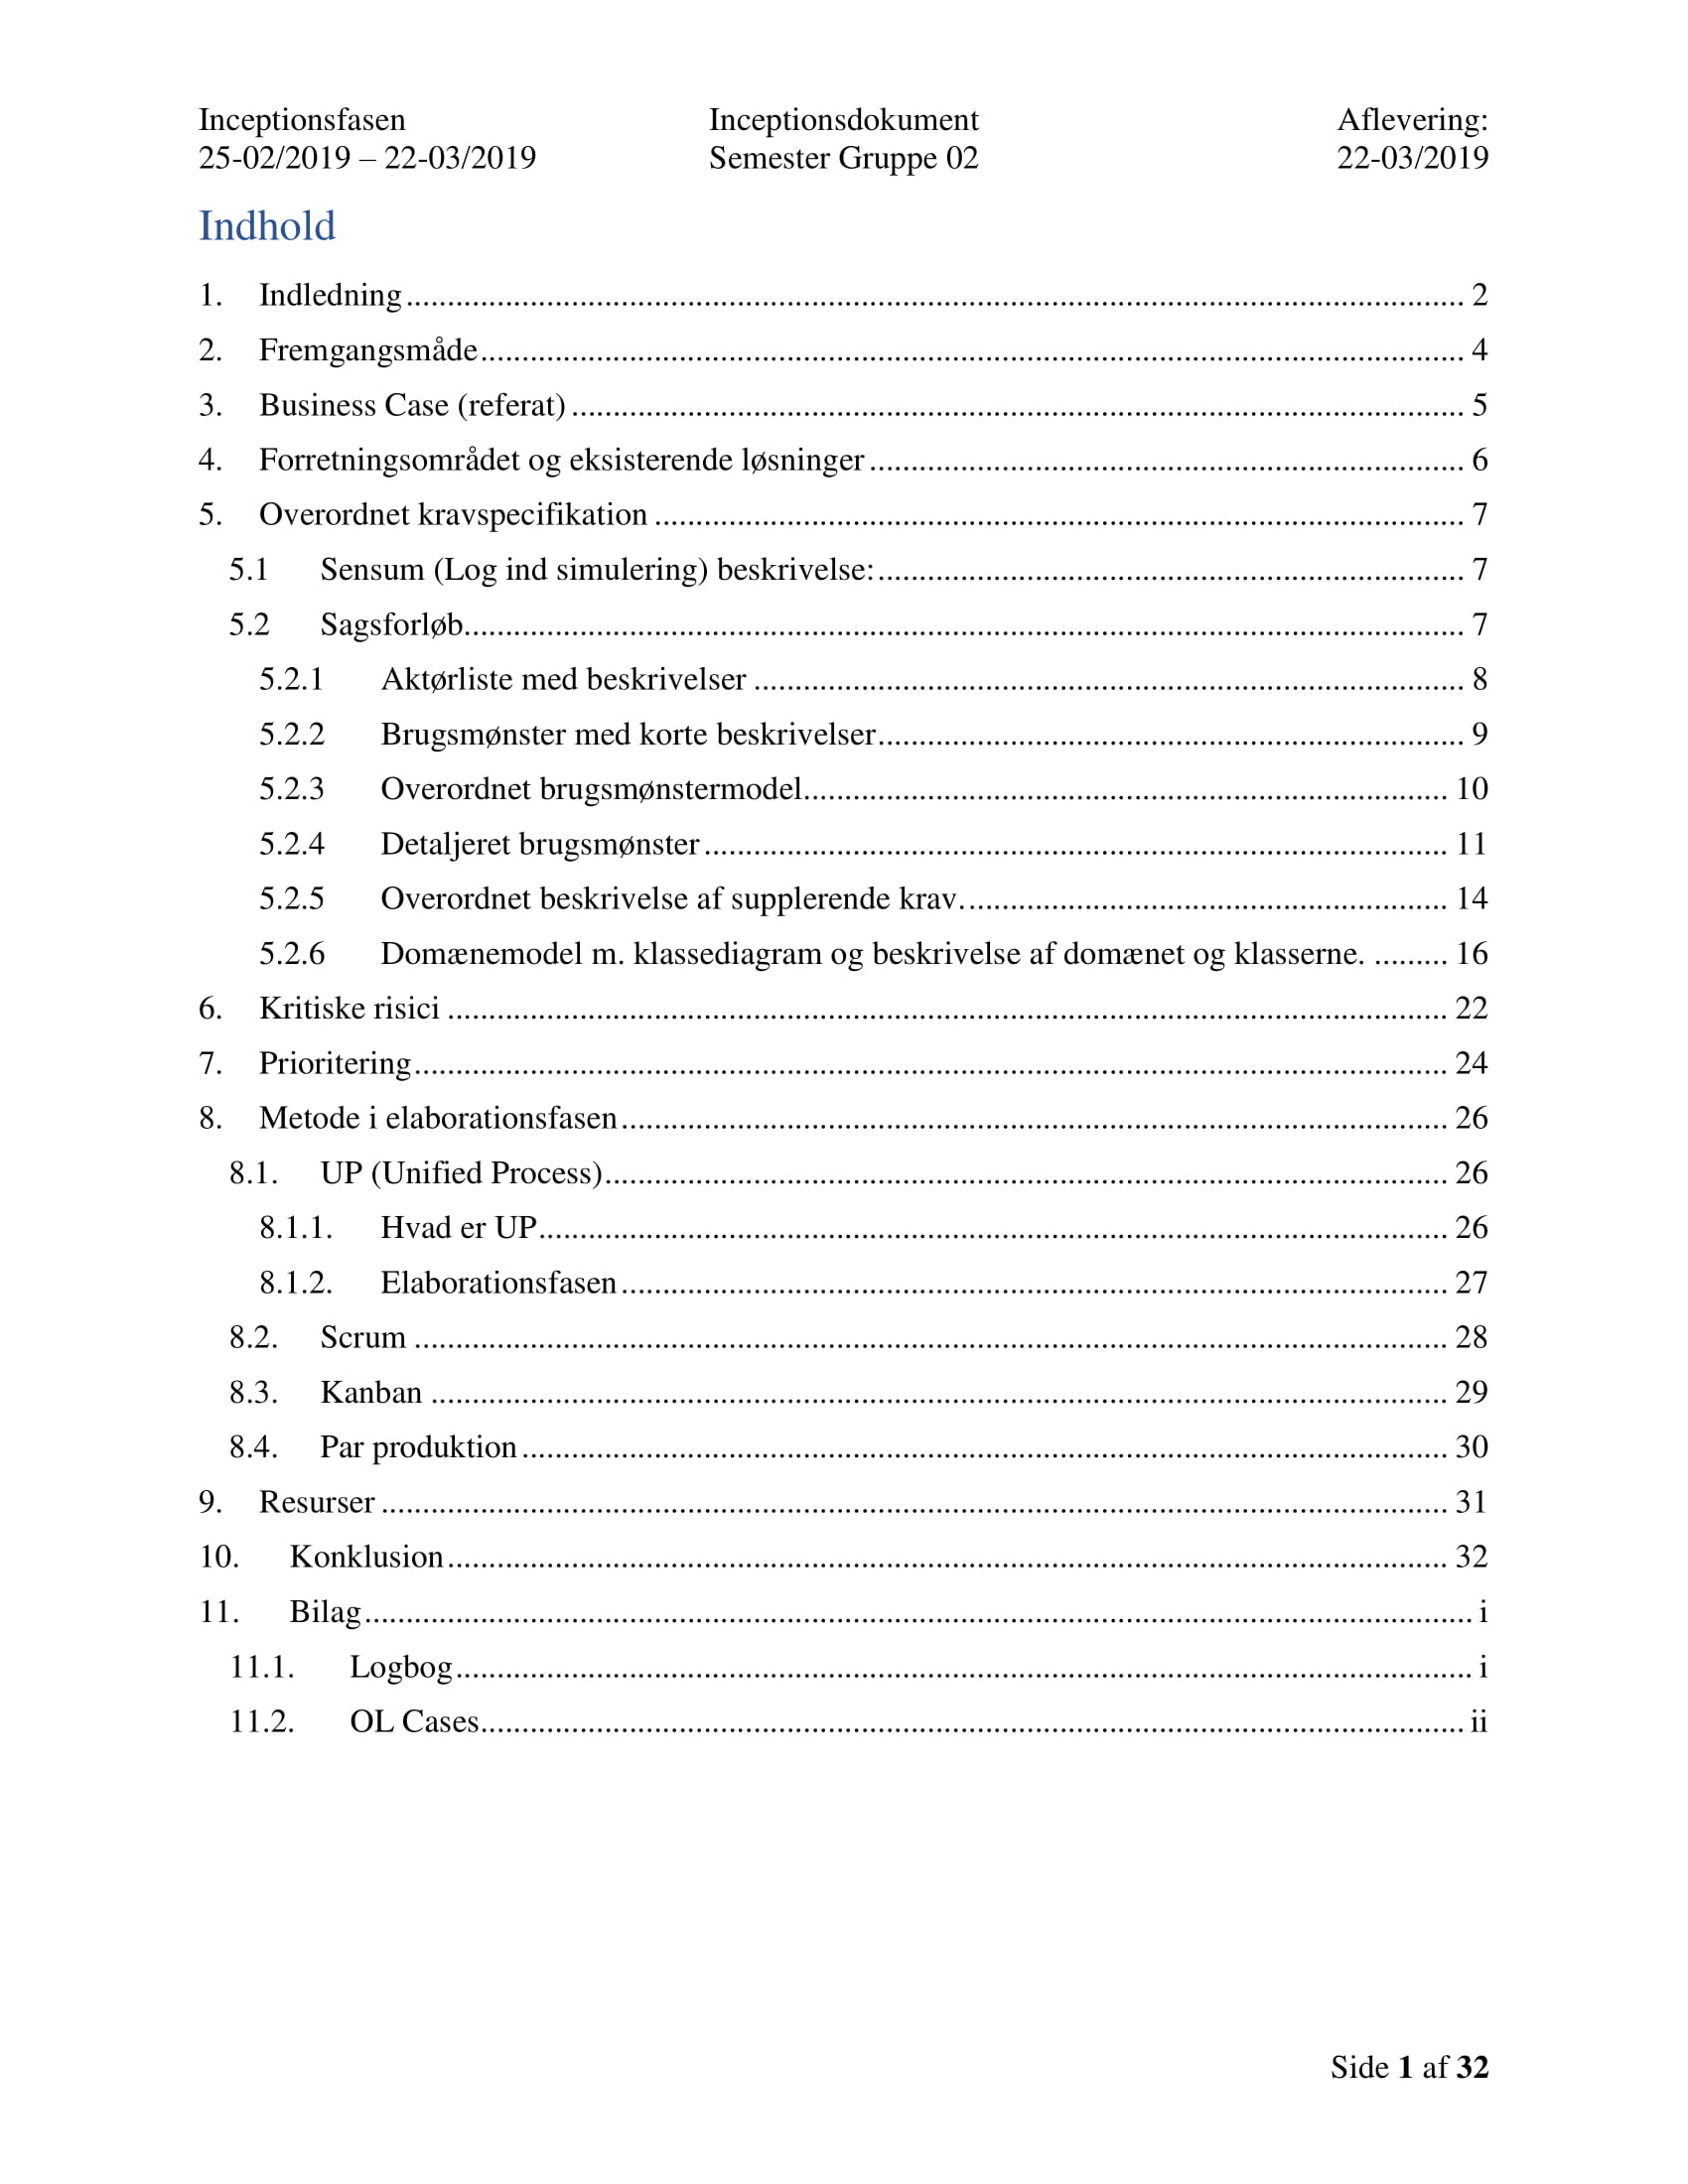
\includegraphics[width=\linewidth]{./PNG/Inceptions/Gruppe 02 + InceptionsDokument-02.jpg} 
\end{figure}

\begin{figure}[hb]
  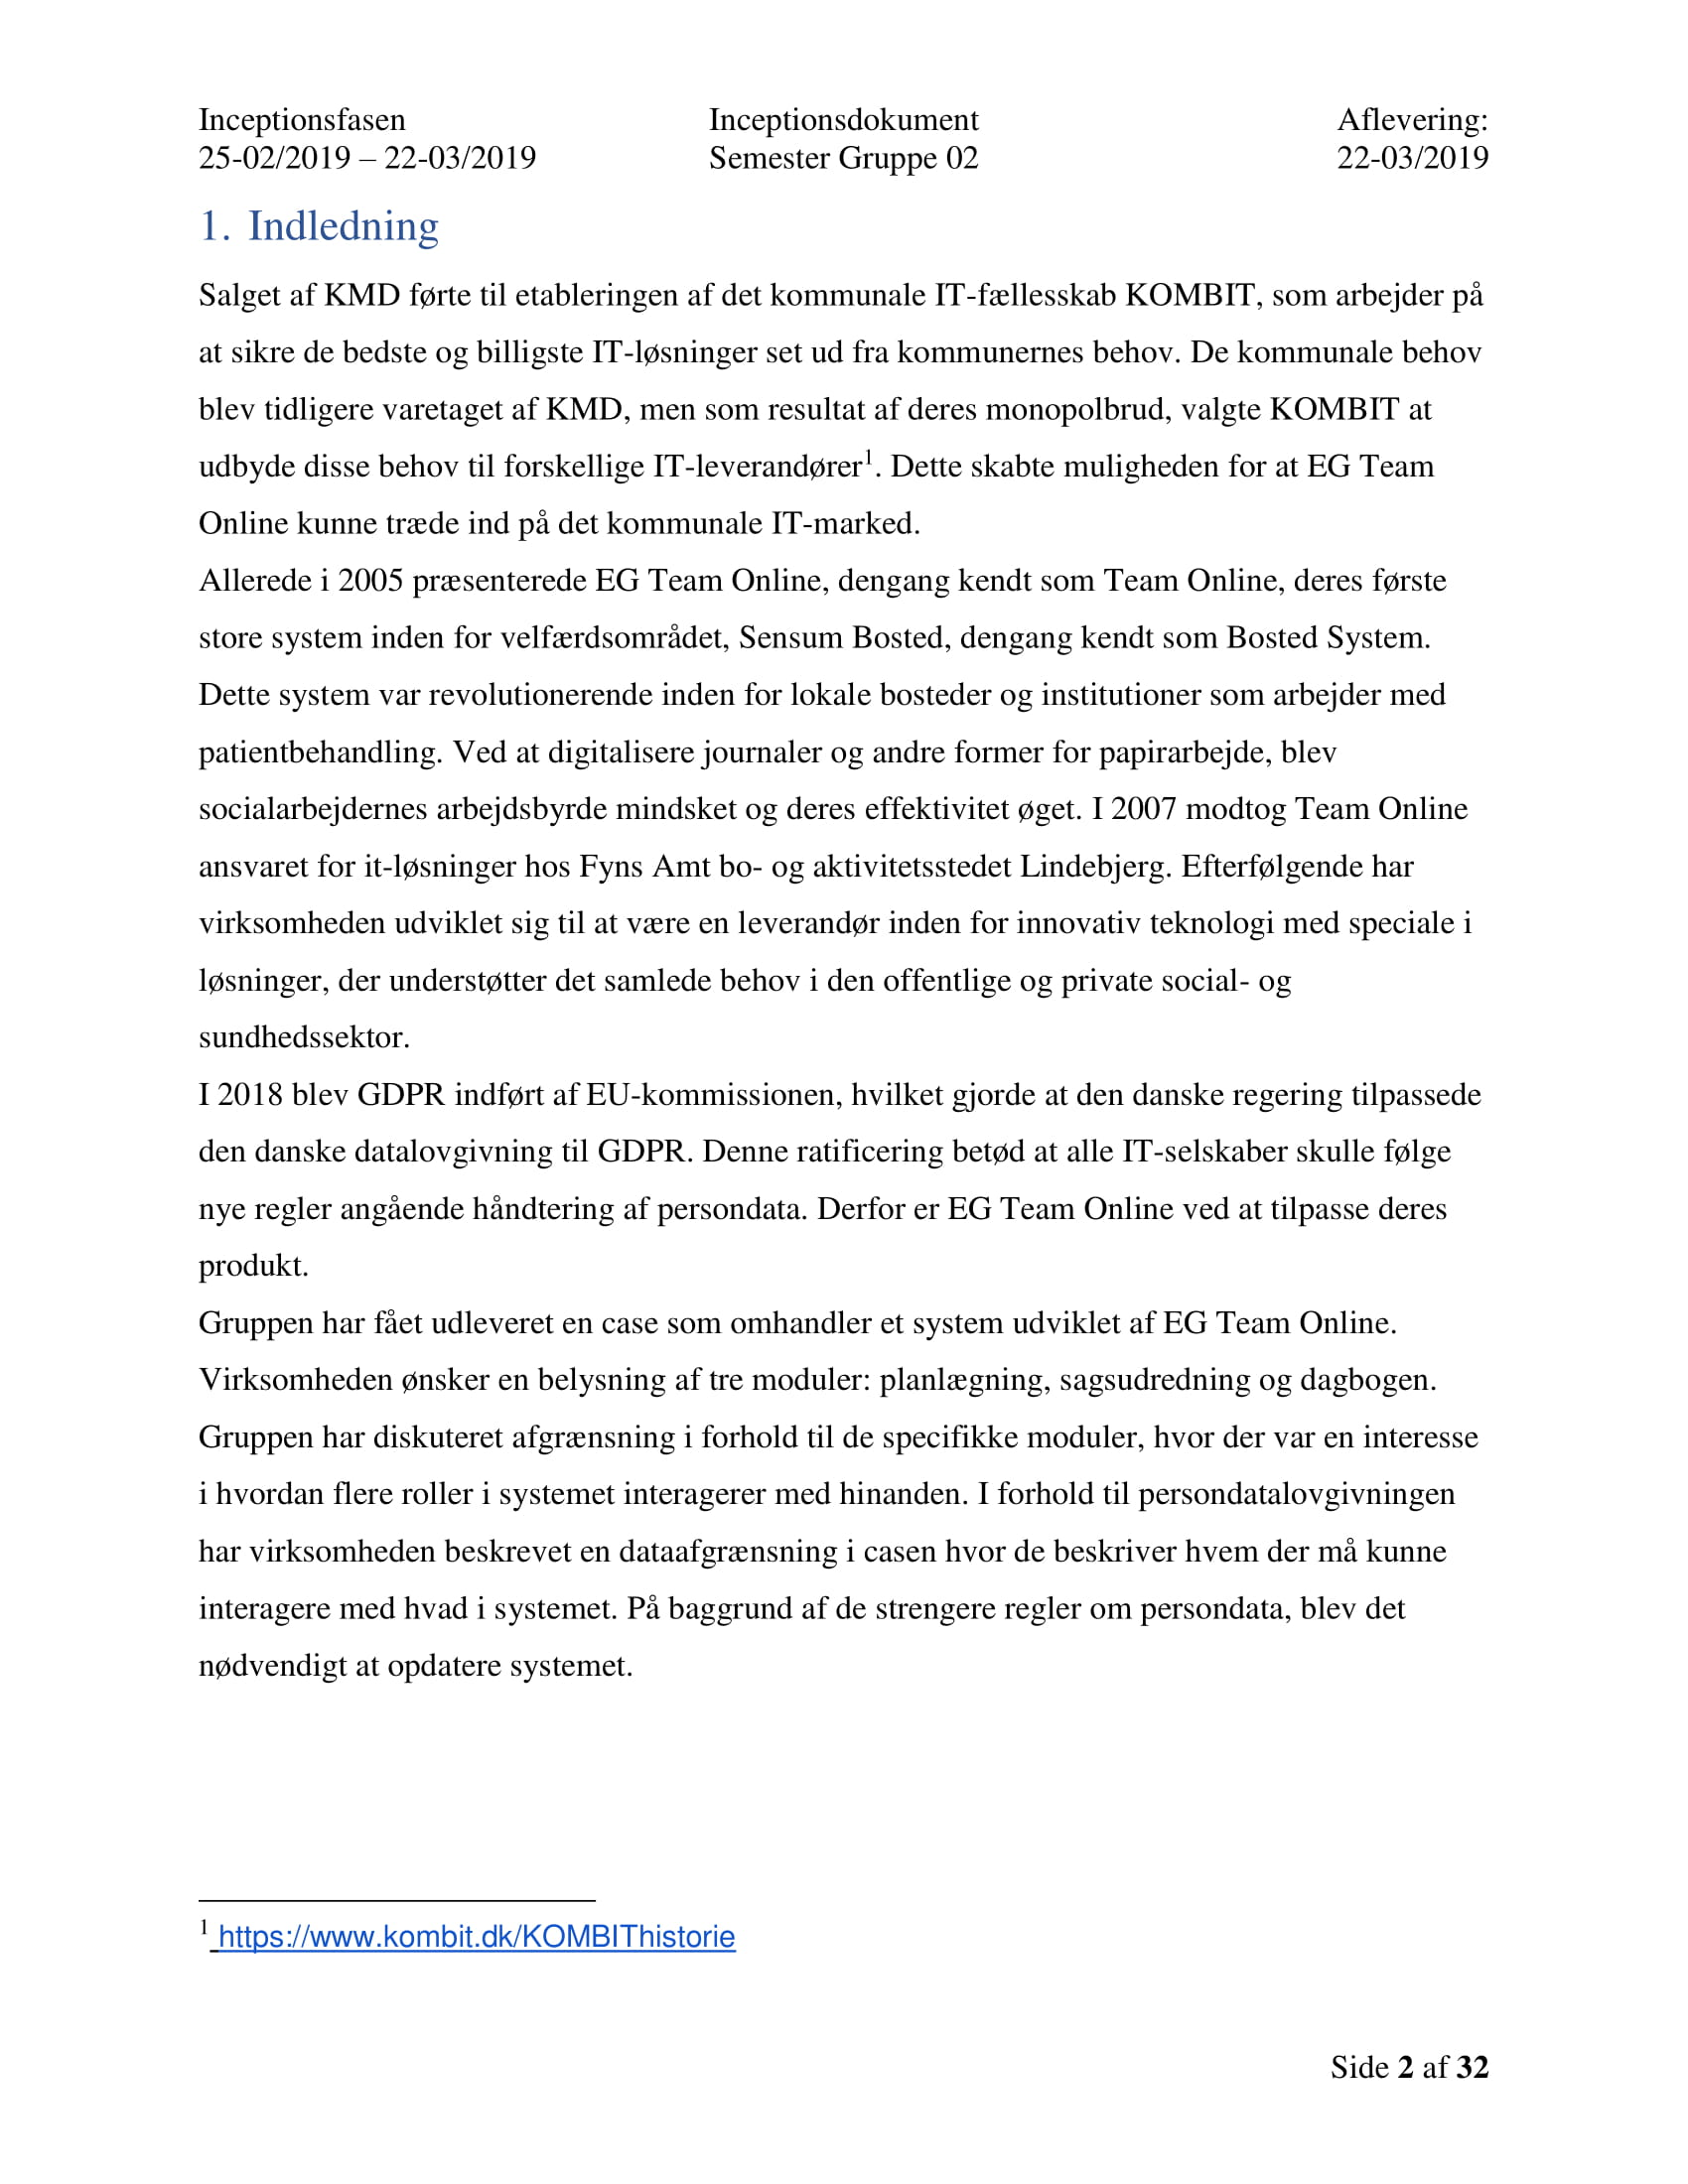
\includegraphics[scale = 0.33]{./PNG/Inceptions/Gruppe 02 + InceptionsDokument-03.jpg} 
\end{figure}


\begin{figure}[hb]
  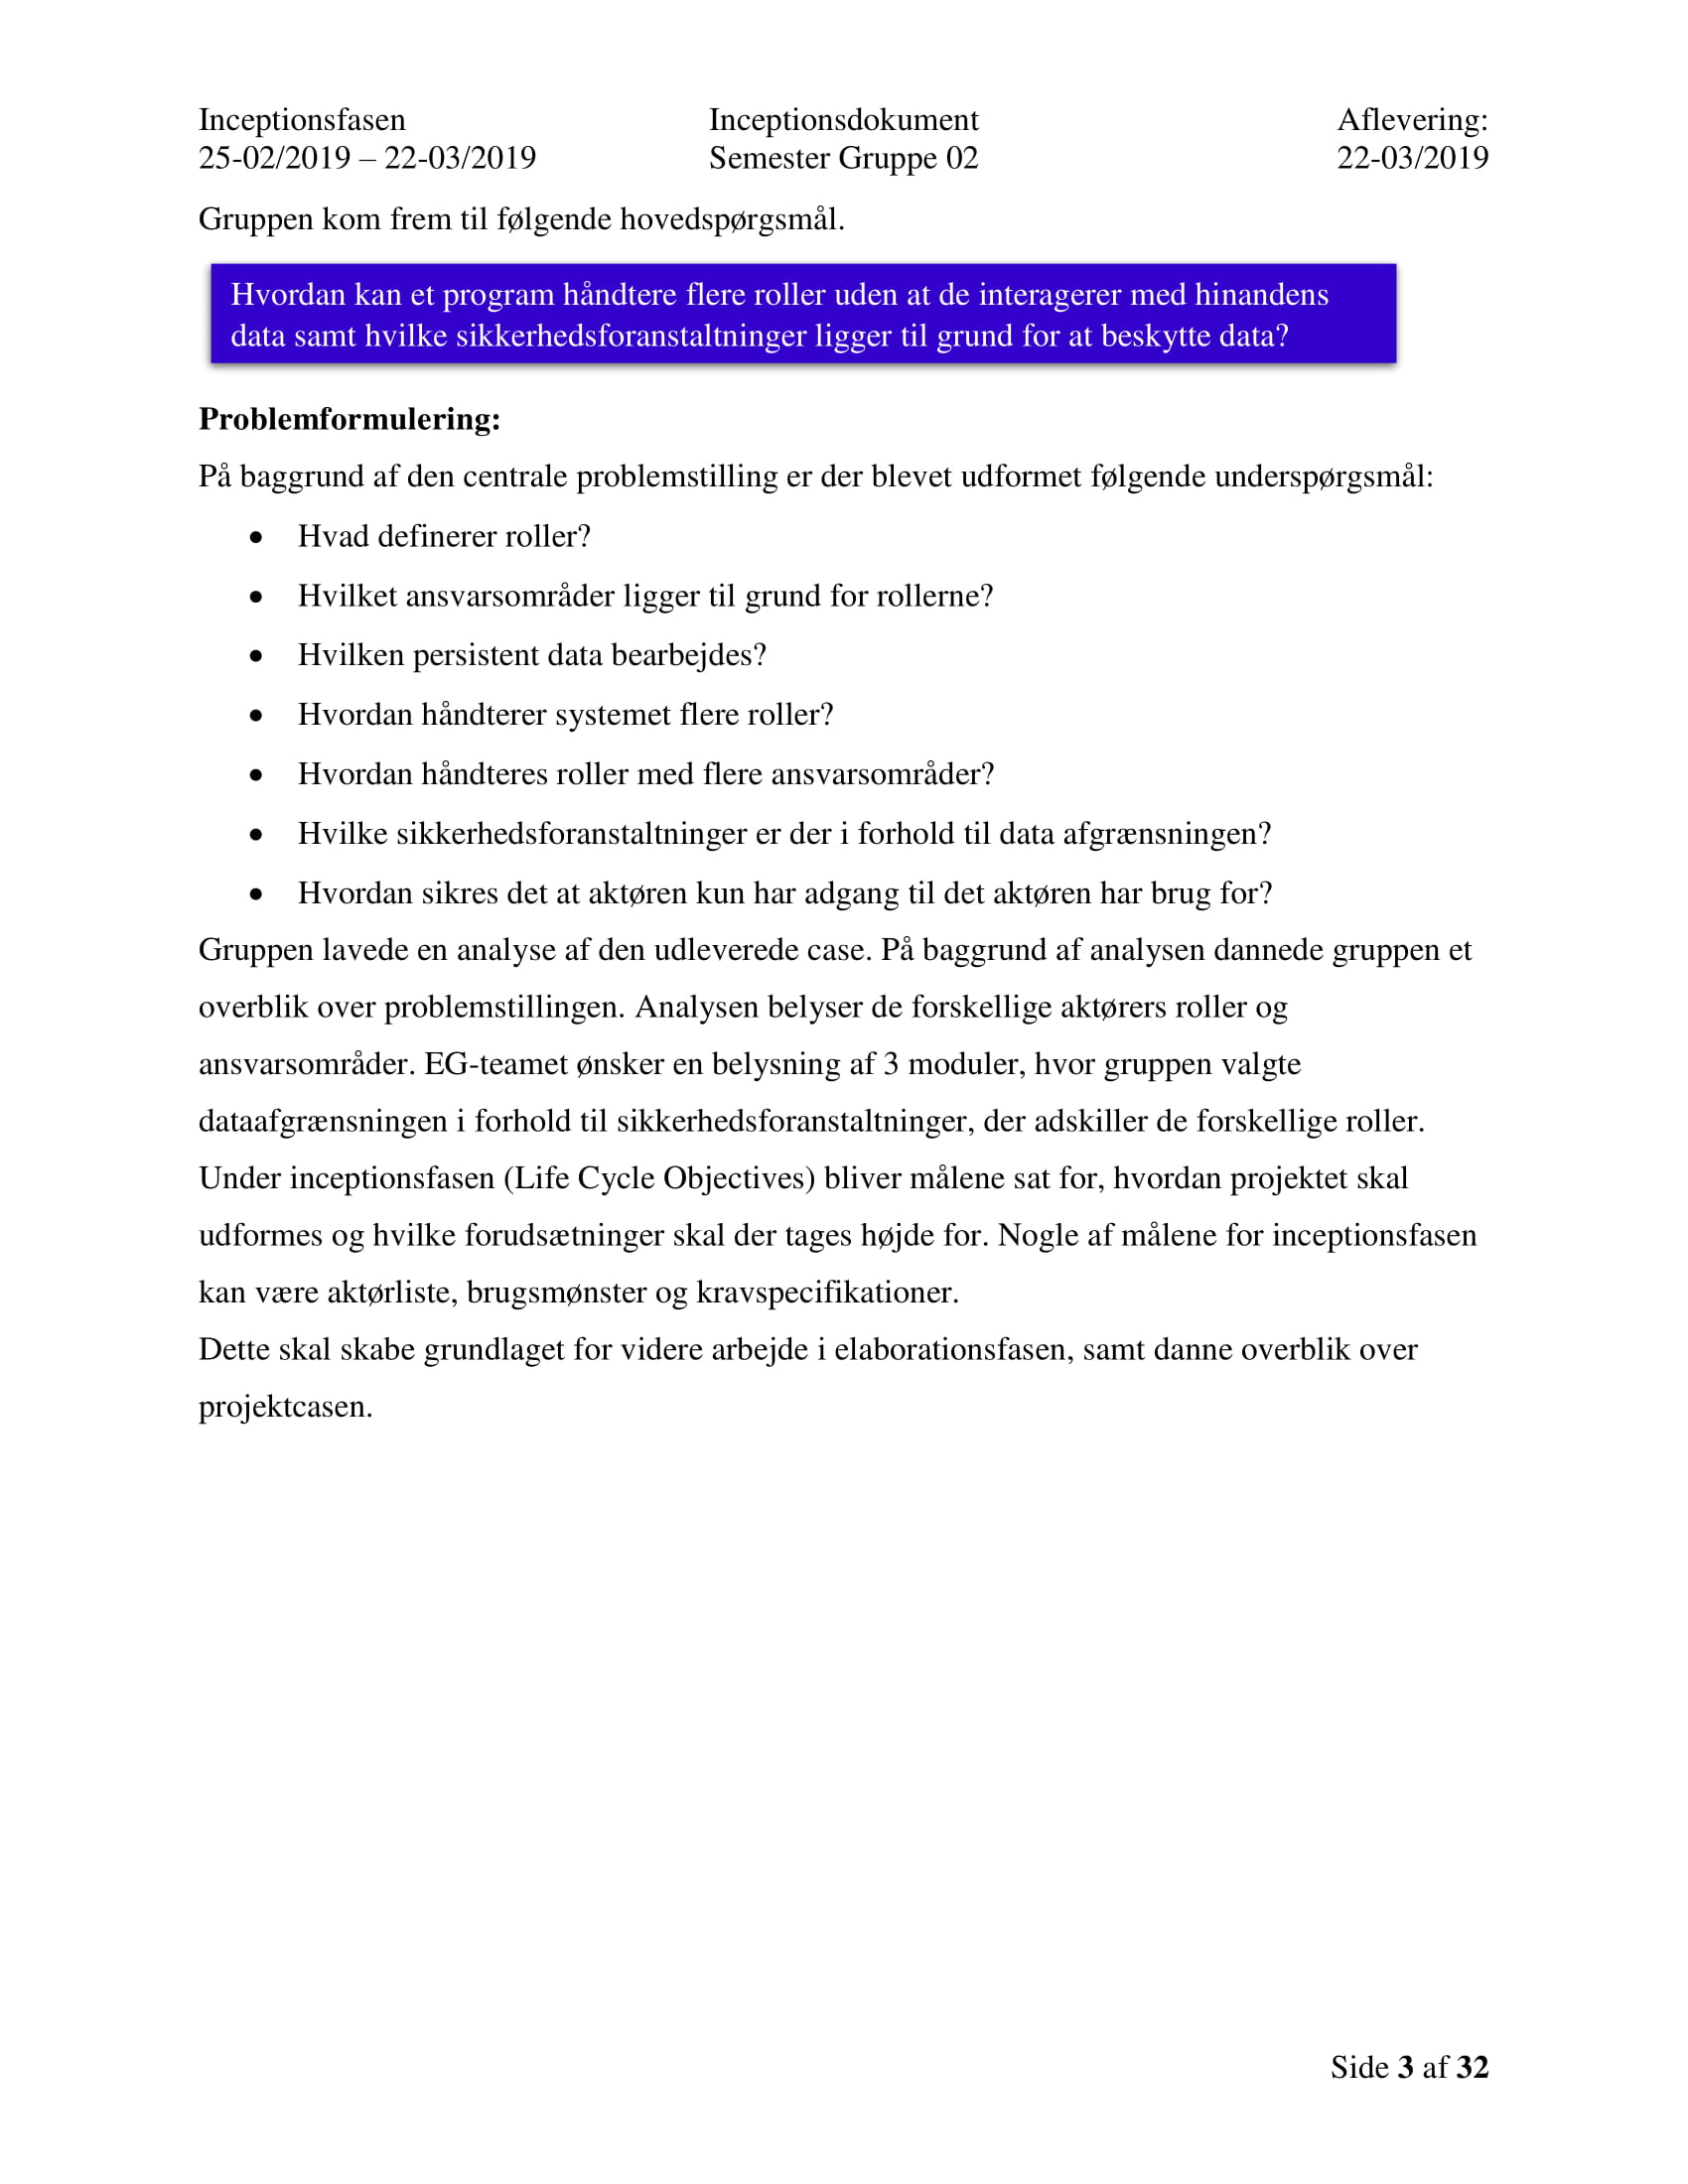
\includegraphics[scale = 0.33]{./PNG/Inceptions/Gruppe 02 + InceptionsDokument-04.jpg} 
\end{figure}

\begin{figure}[hb]
  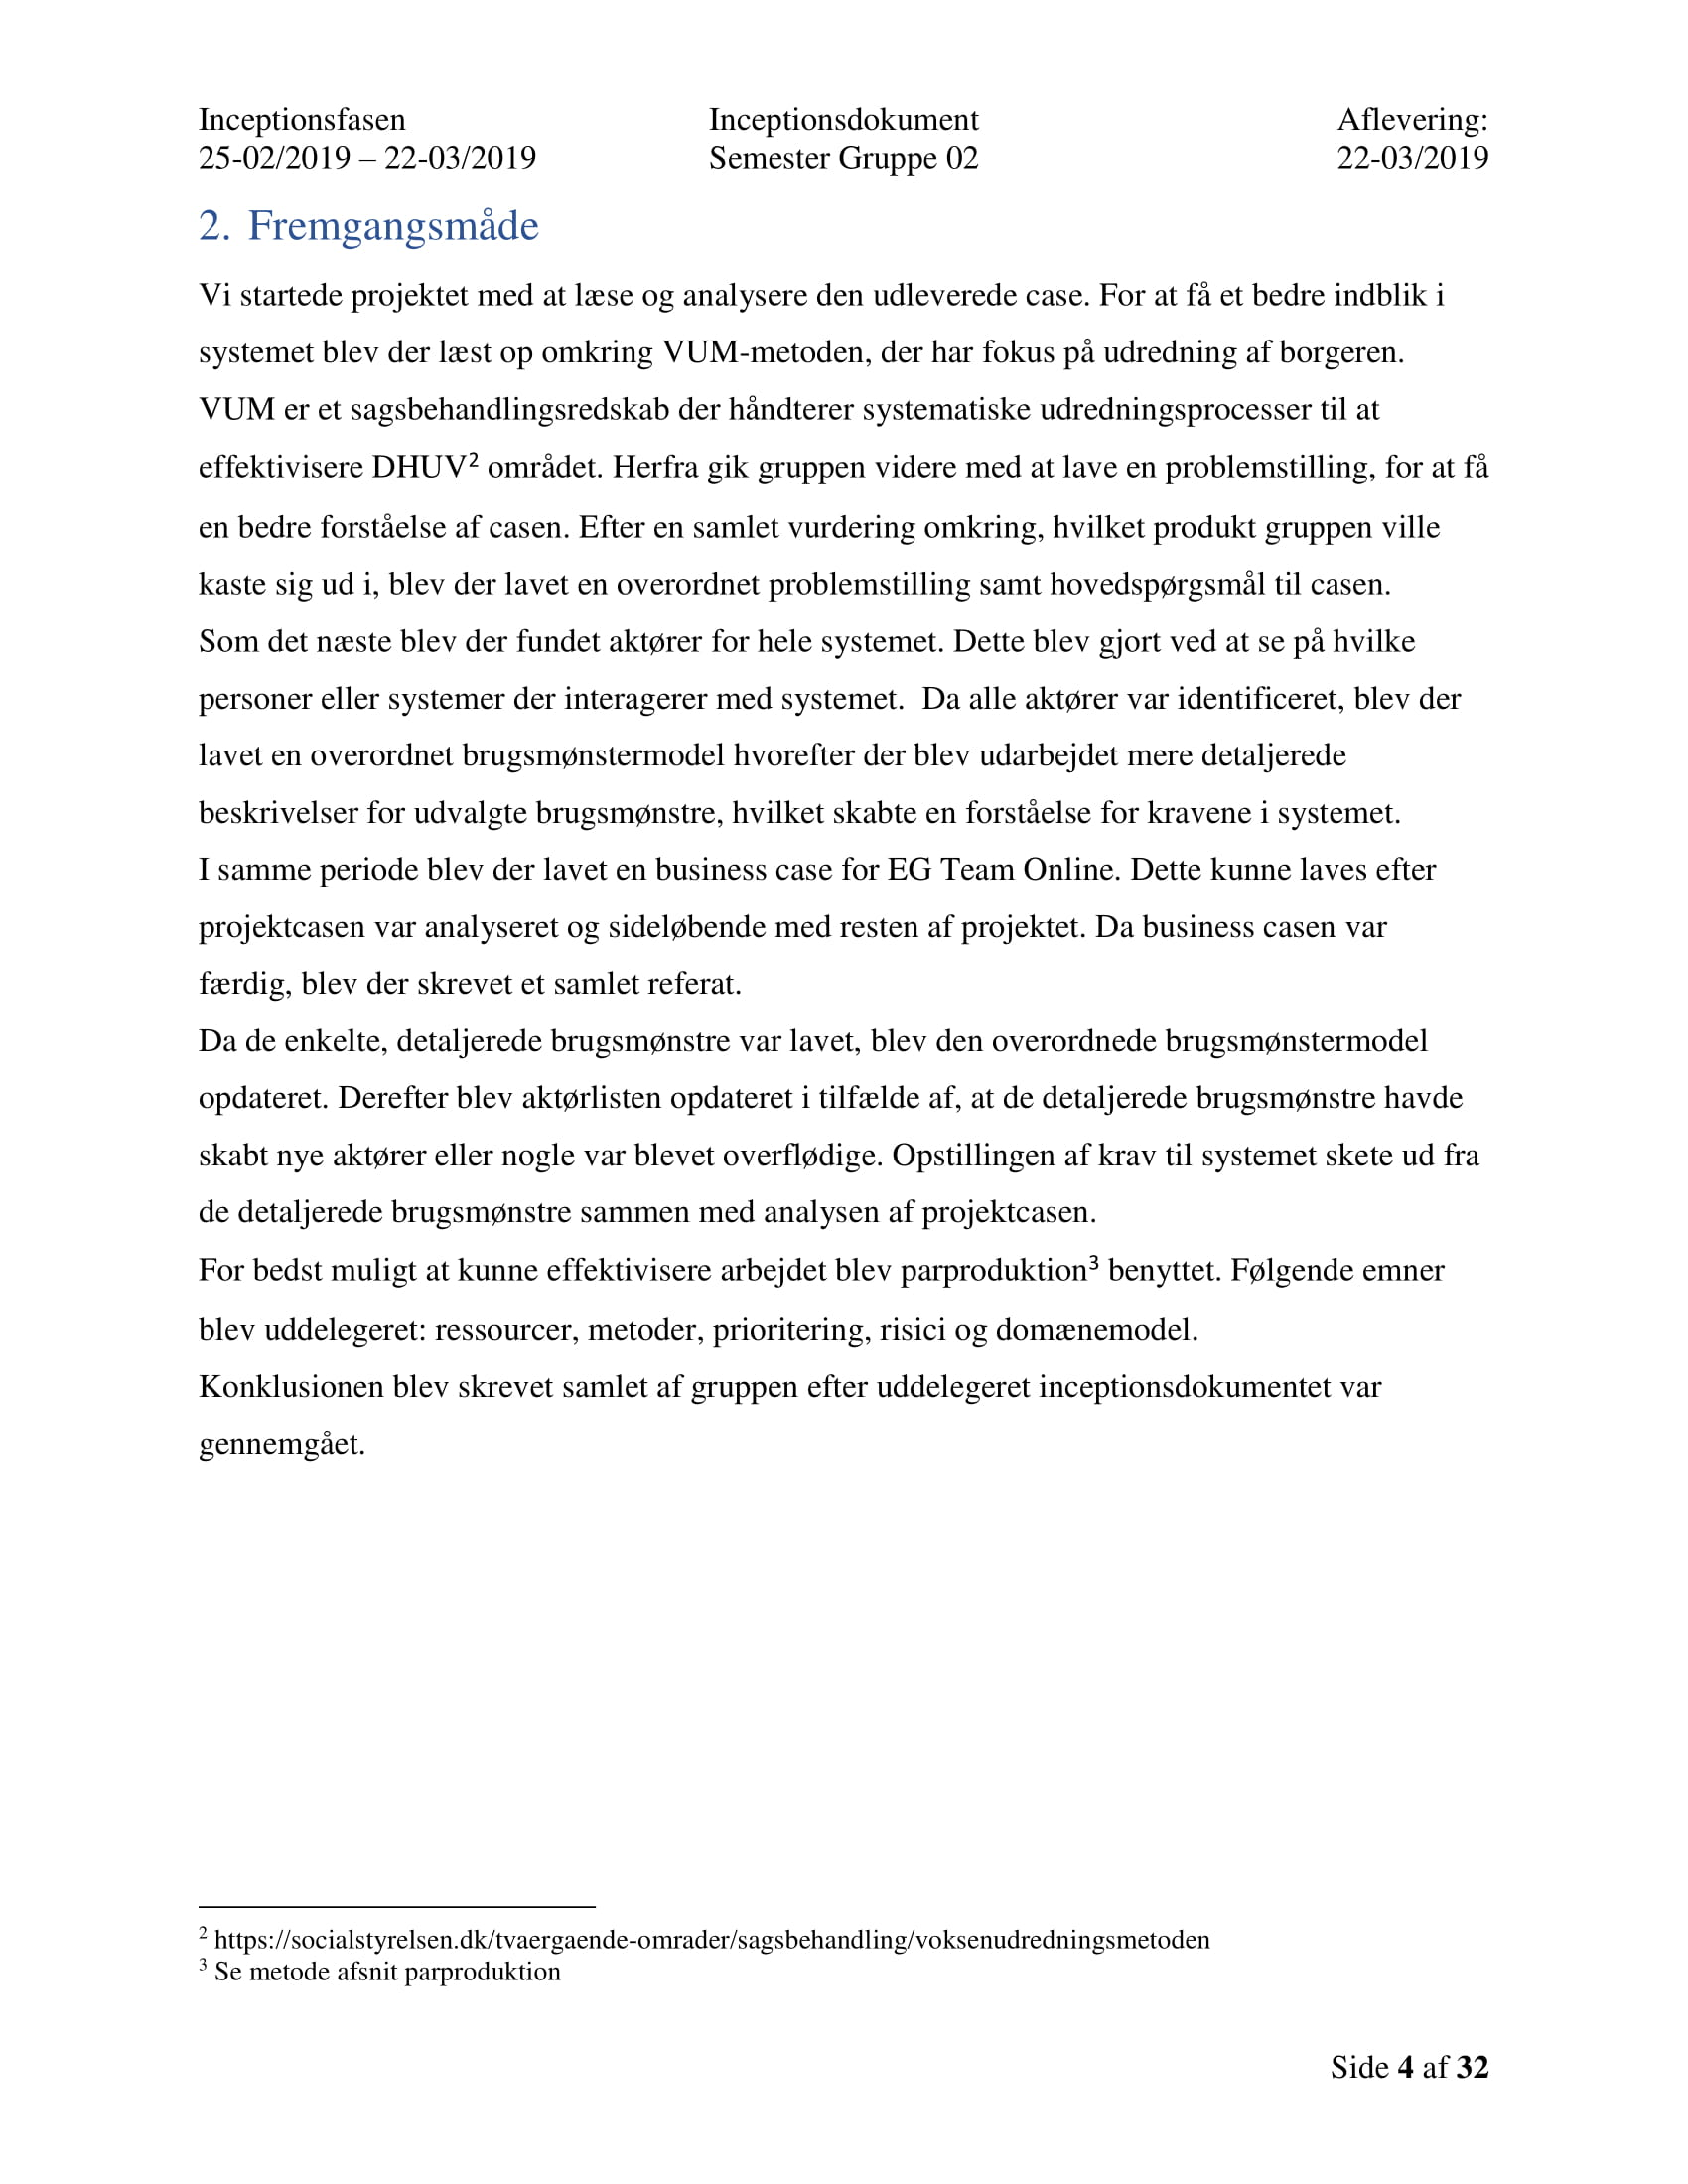
\includegraphics[scale = 0.33]{./PNG/Inceptions/Gruppe 02 + InceptionsDokument-05.jpg} 
\end{figure}

\begin{figure}[hb]
  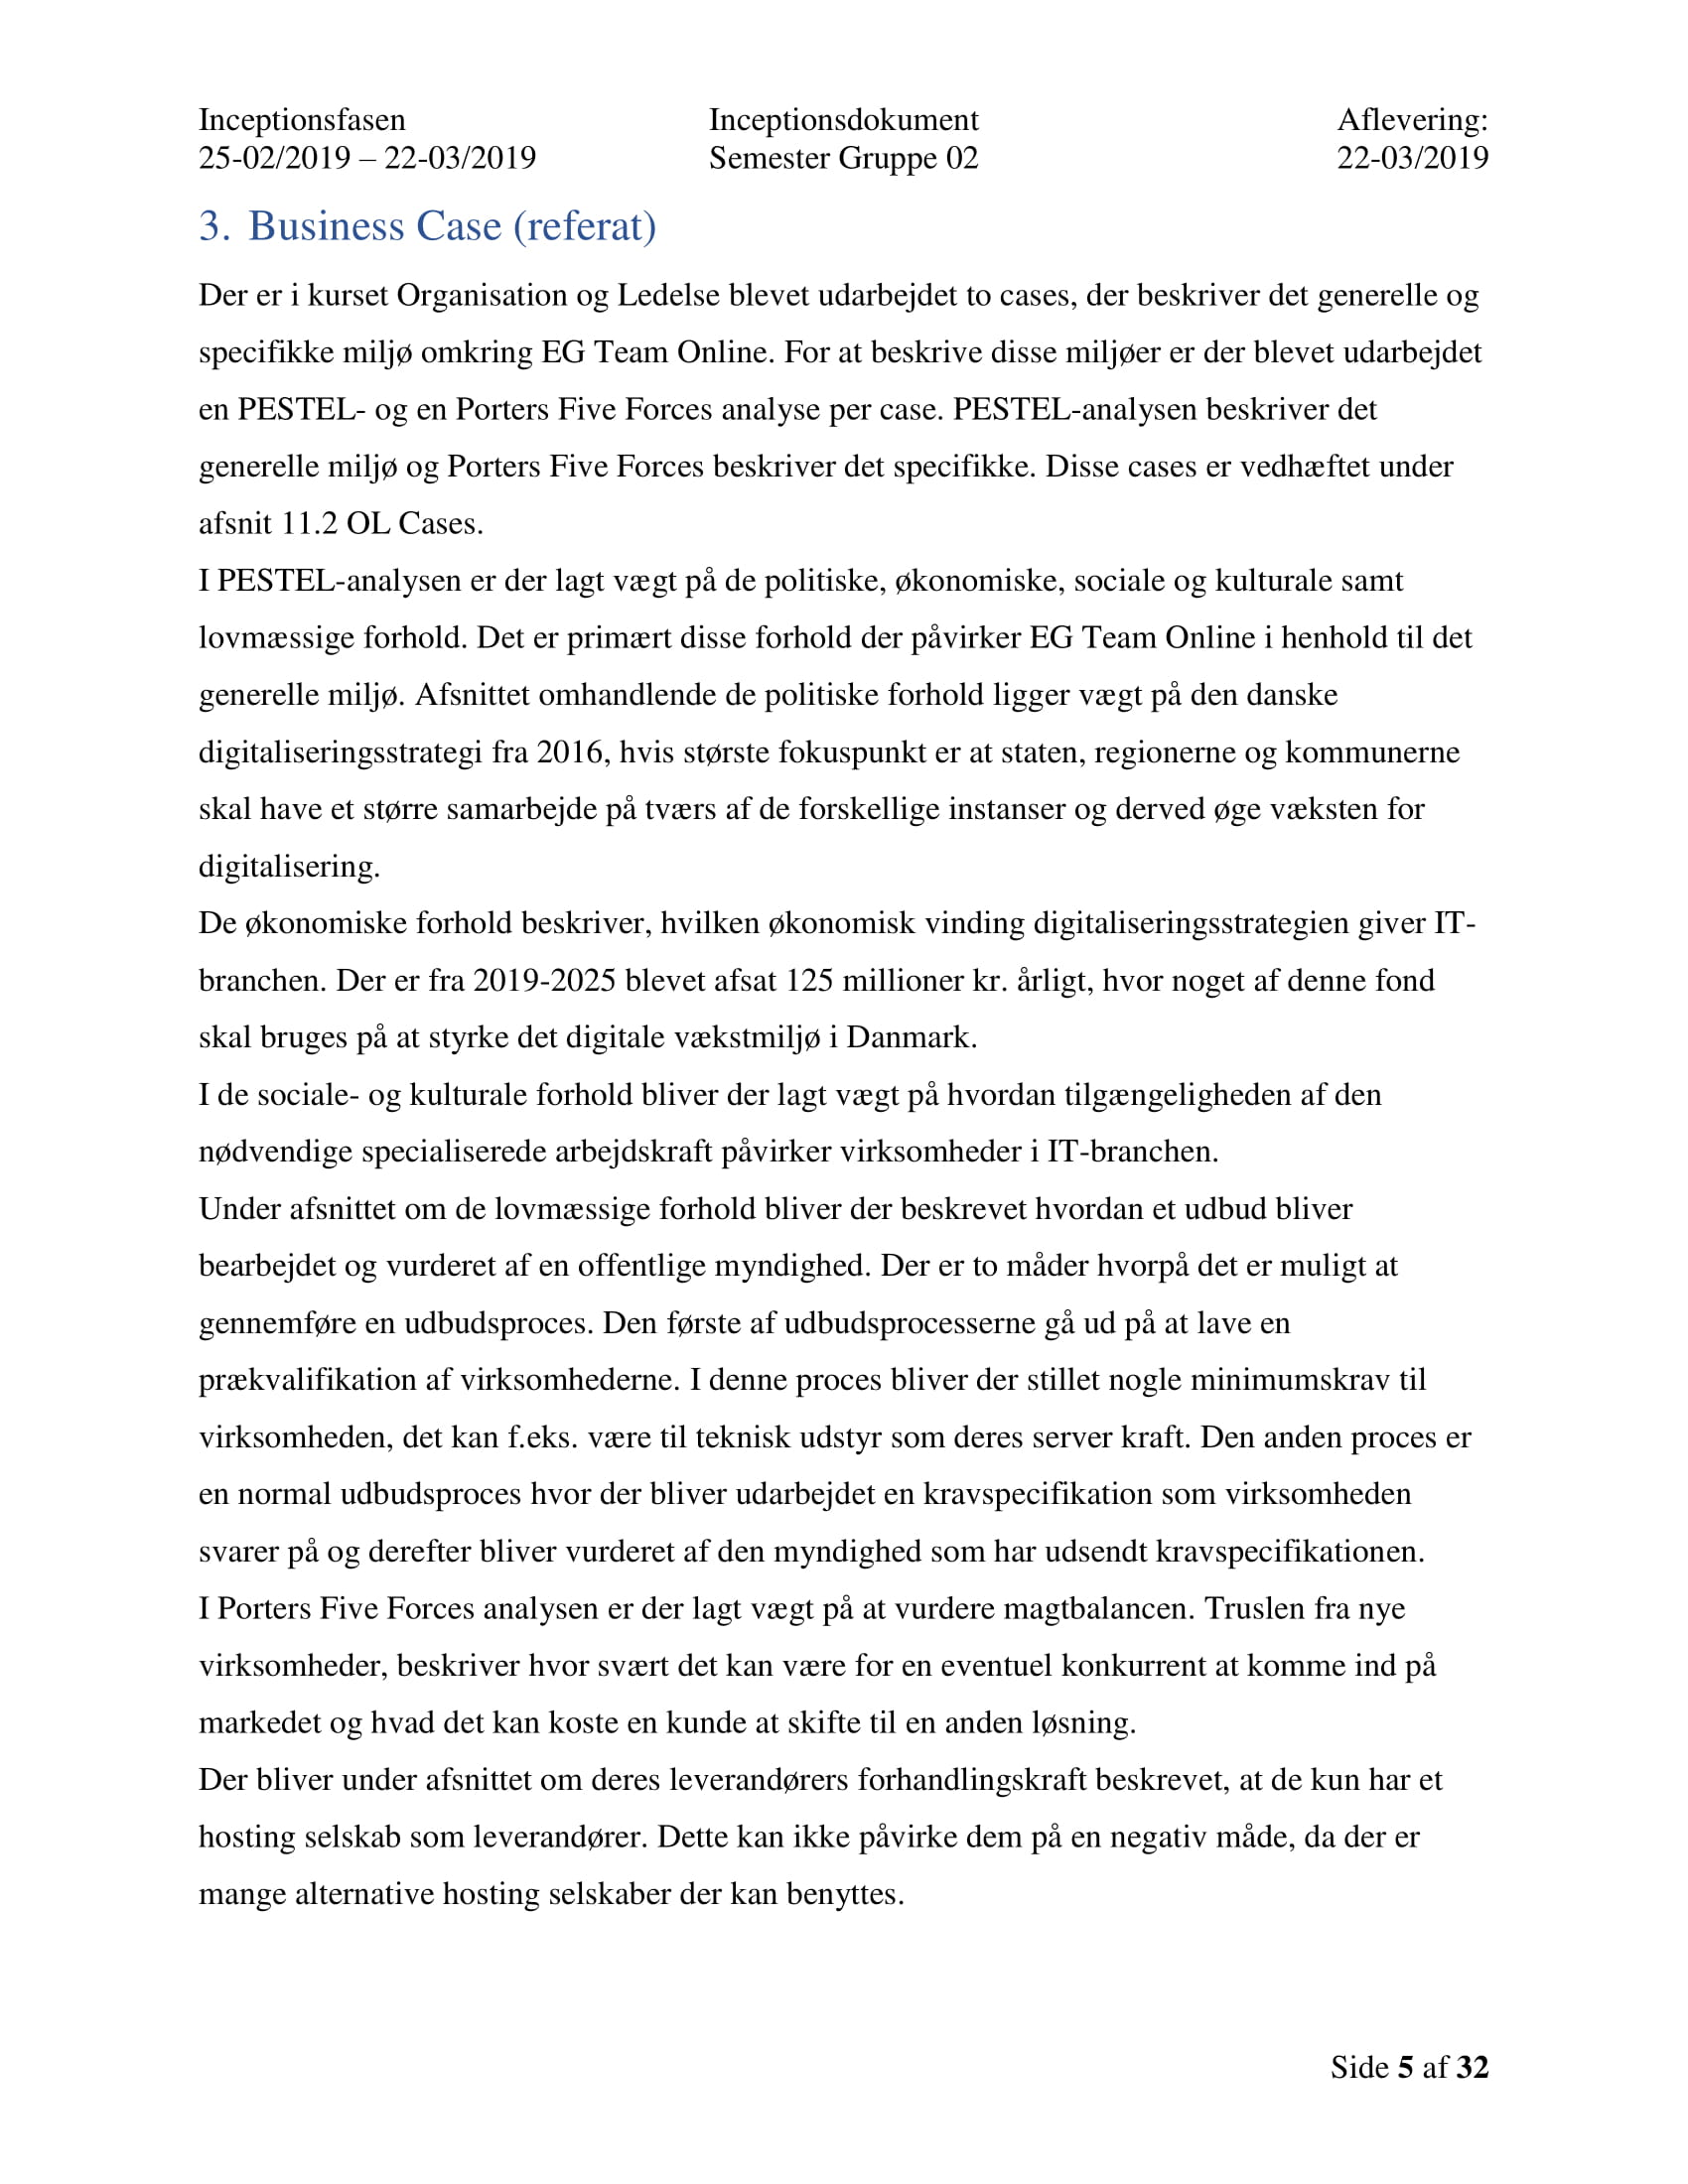
\includegraphics[scale = 0.33]{./PNG/Inceptions/Gruppe 02 + InceptionsDokument-06.jpg} 
\end{figure}

\begin{figure}[hb]
  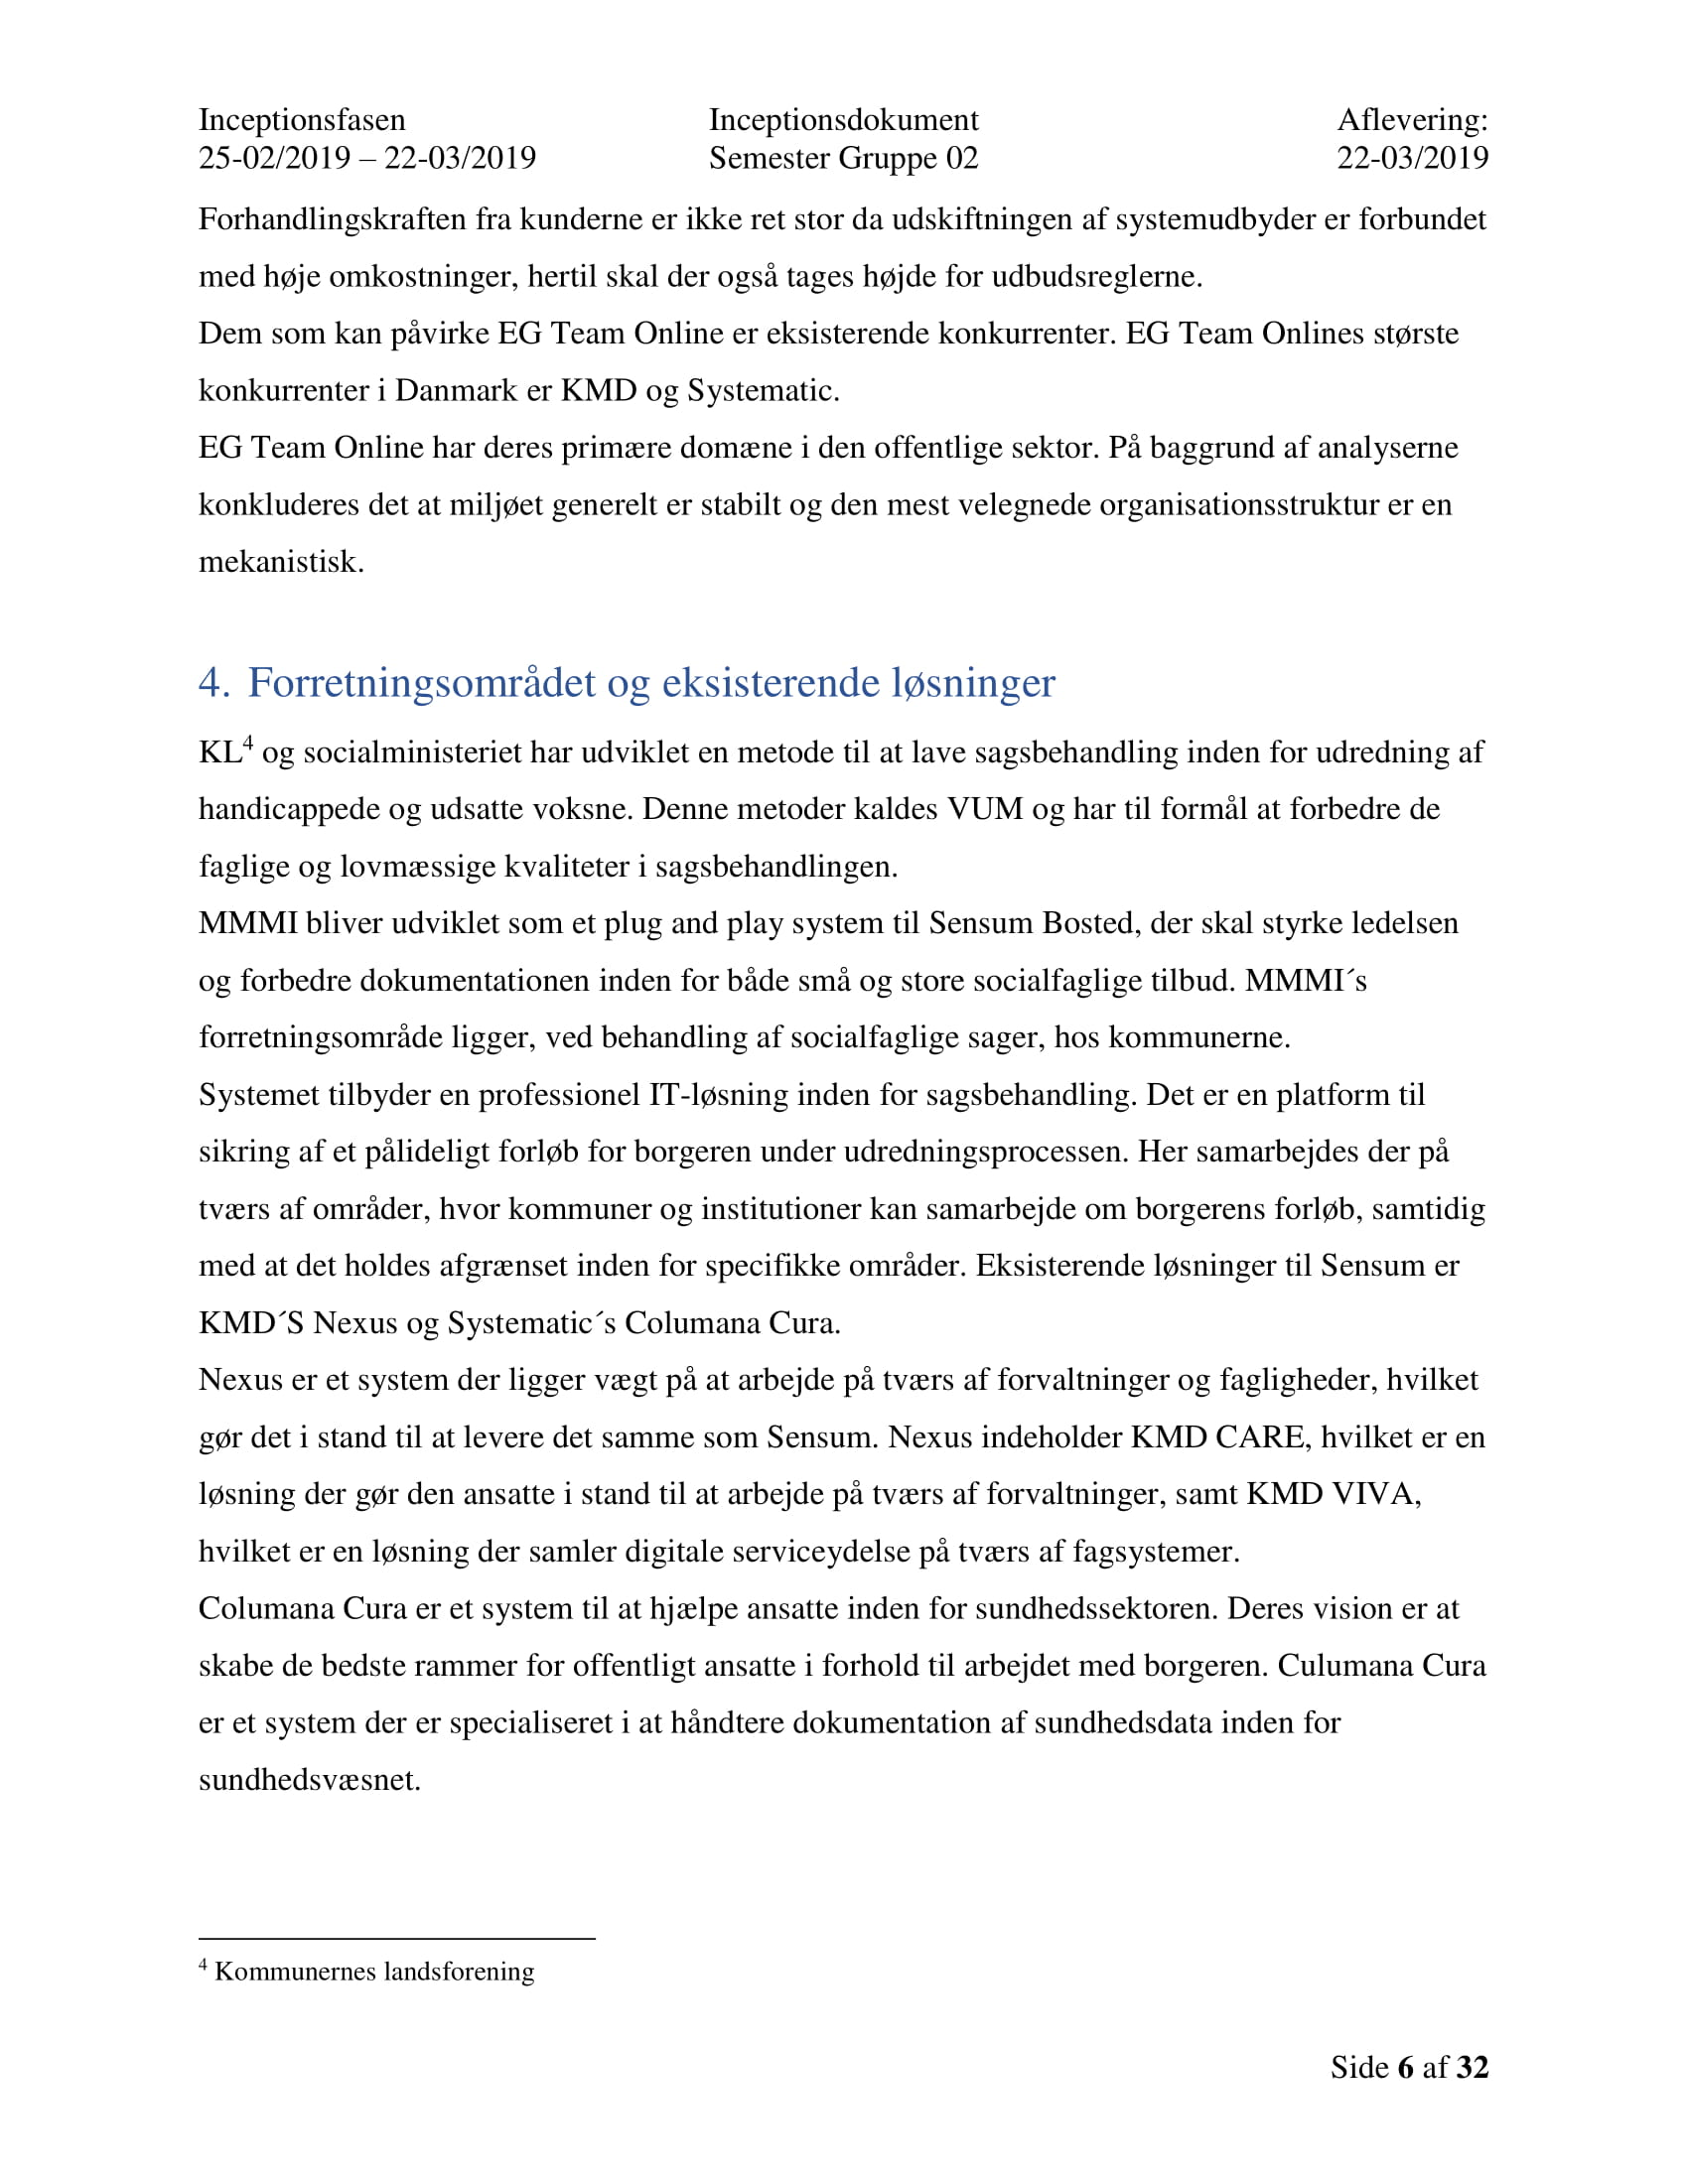
\includegraphics[scale = 0.33]{./PNG/Inceptions/Gruppe 02 + InceptionsDokument-07.jpg} 
\end{figure}

\begin{figure}[hb]
  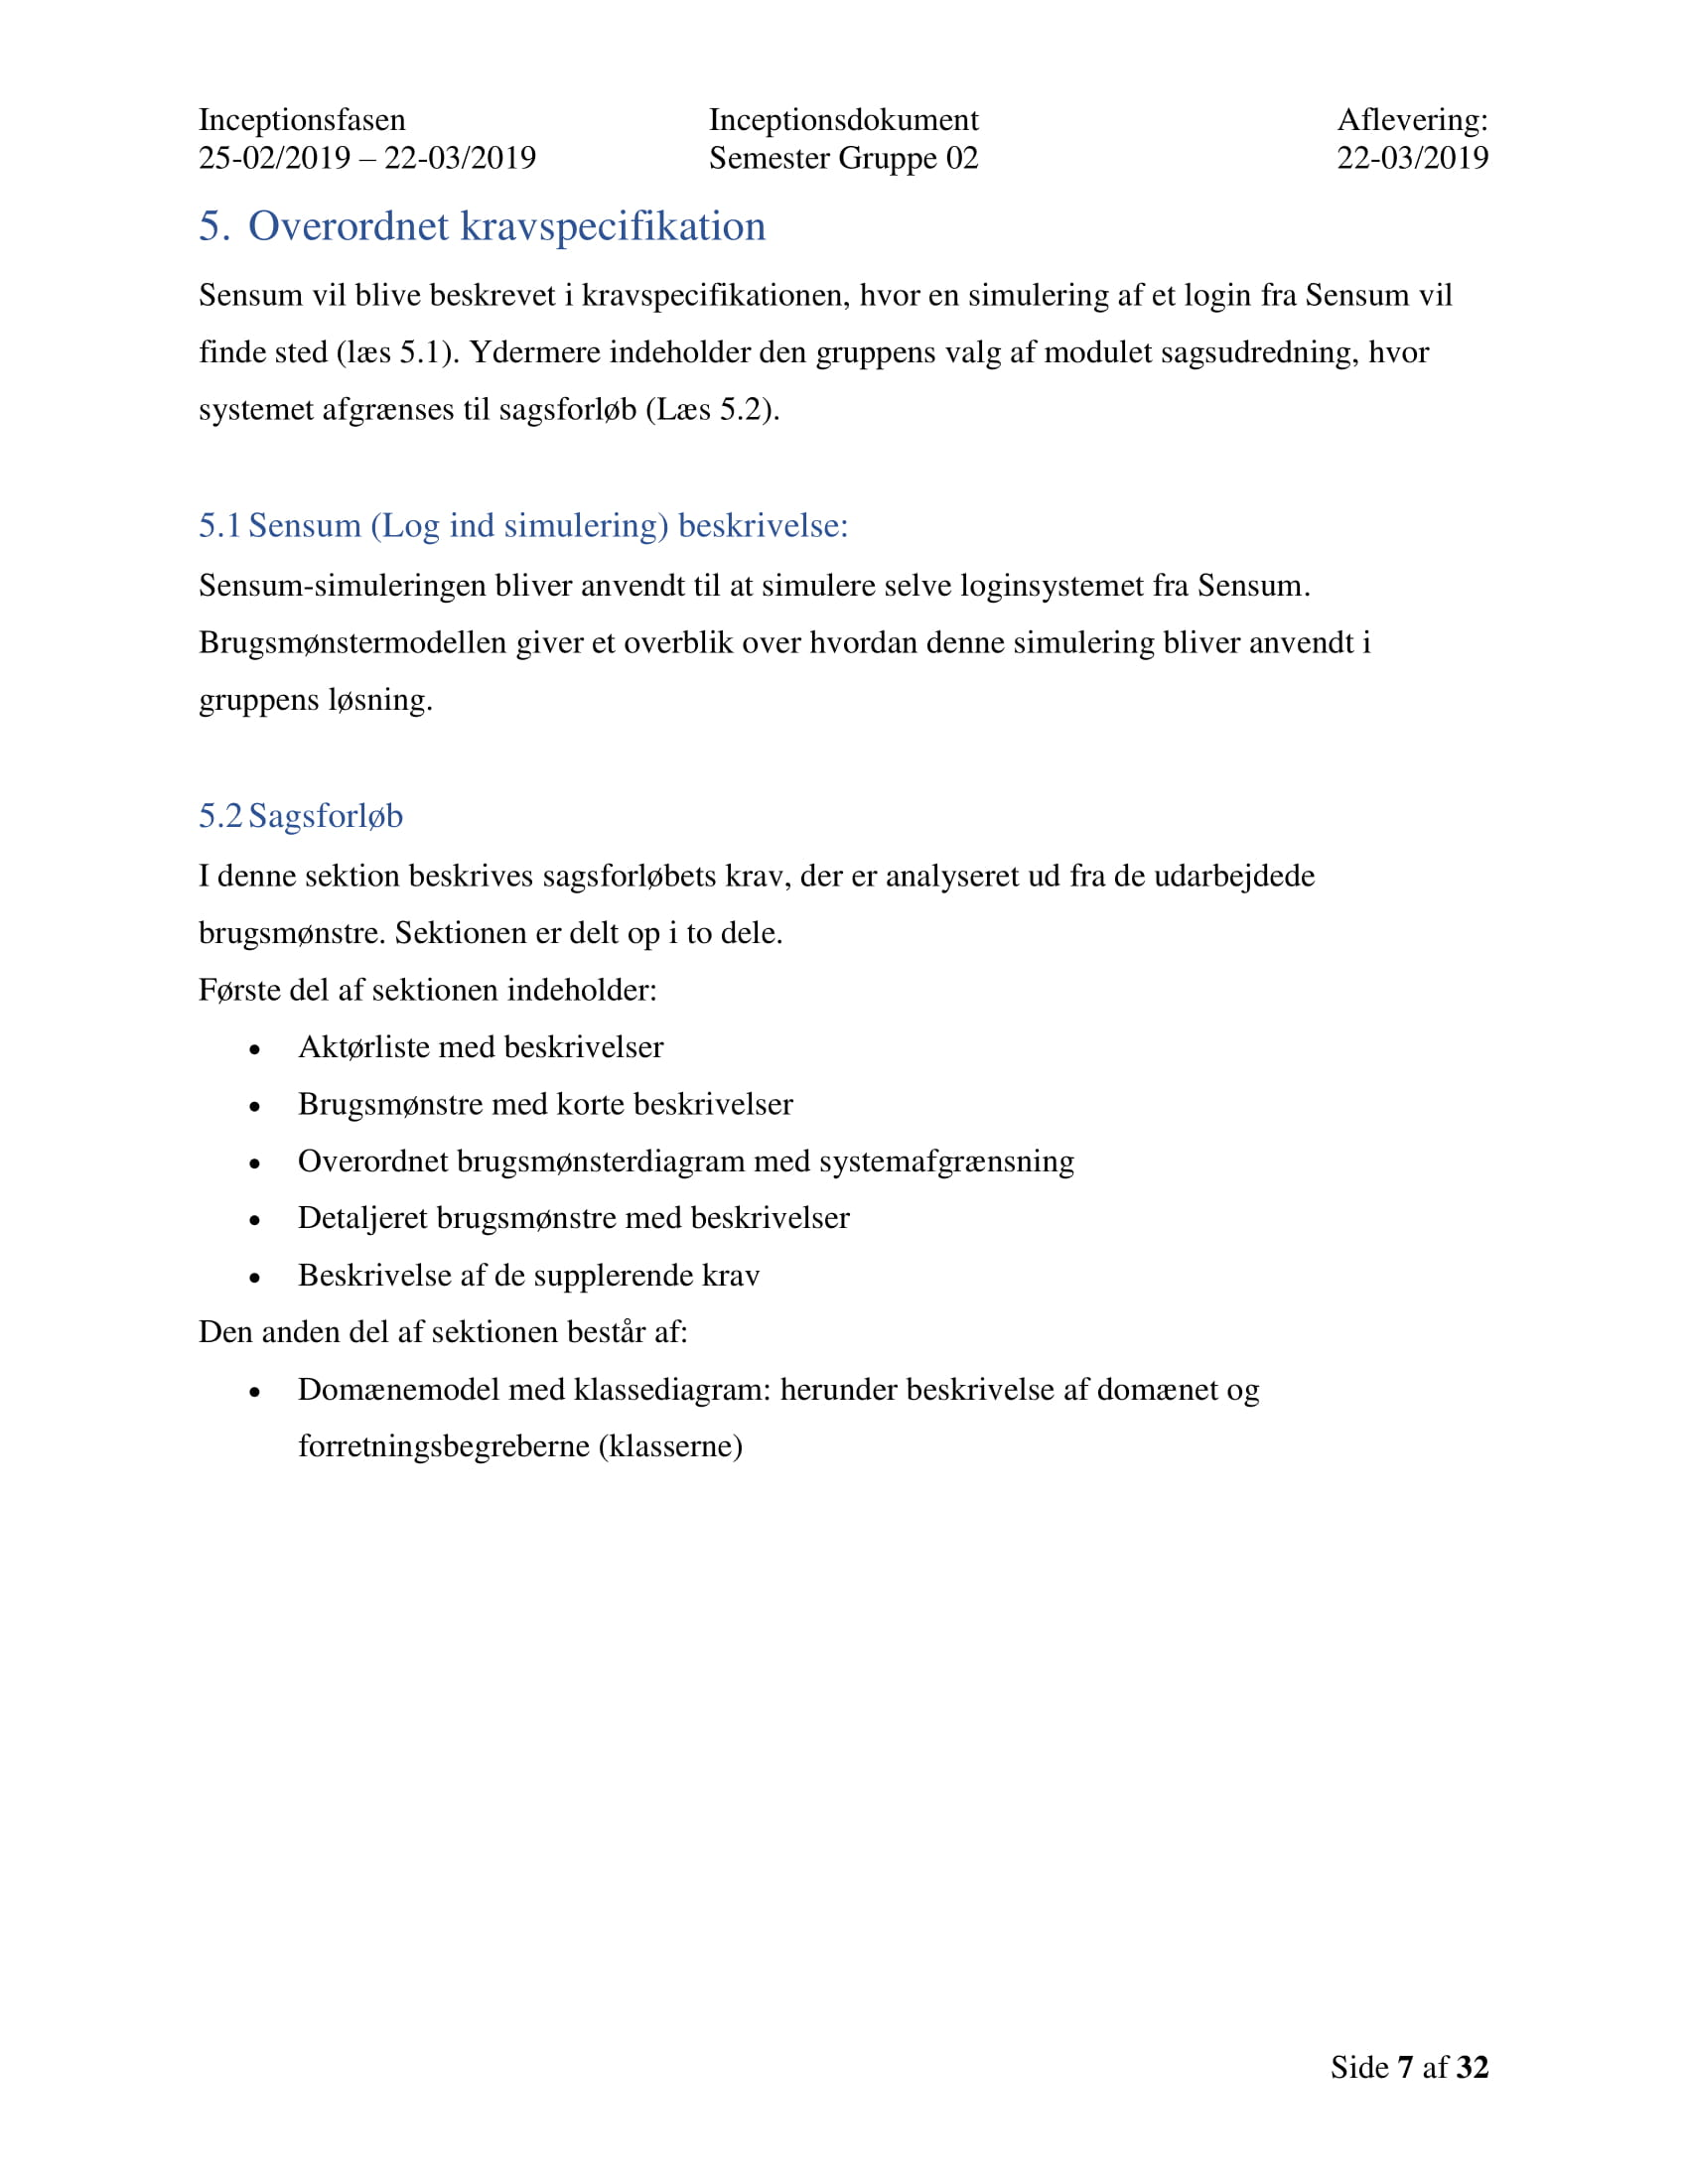
\includegraphics[scale = 0.33]{./PNG/Inceptions/Gruppe 02 + InceptionsDokument-08.jpg} 
\end{figure}

\begin{figure}[hb]
  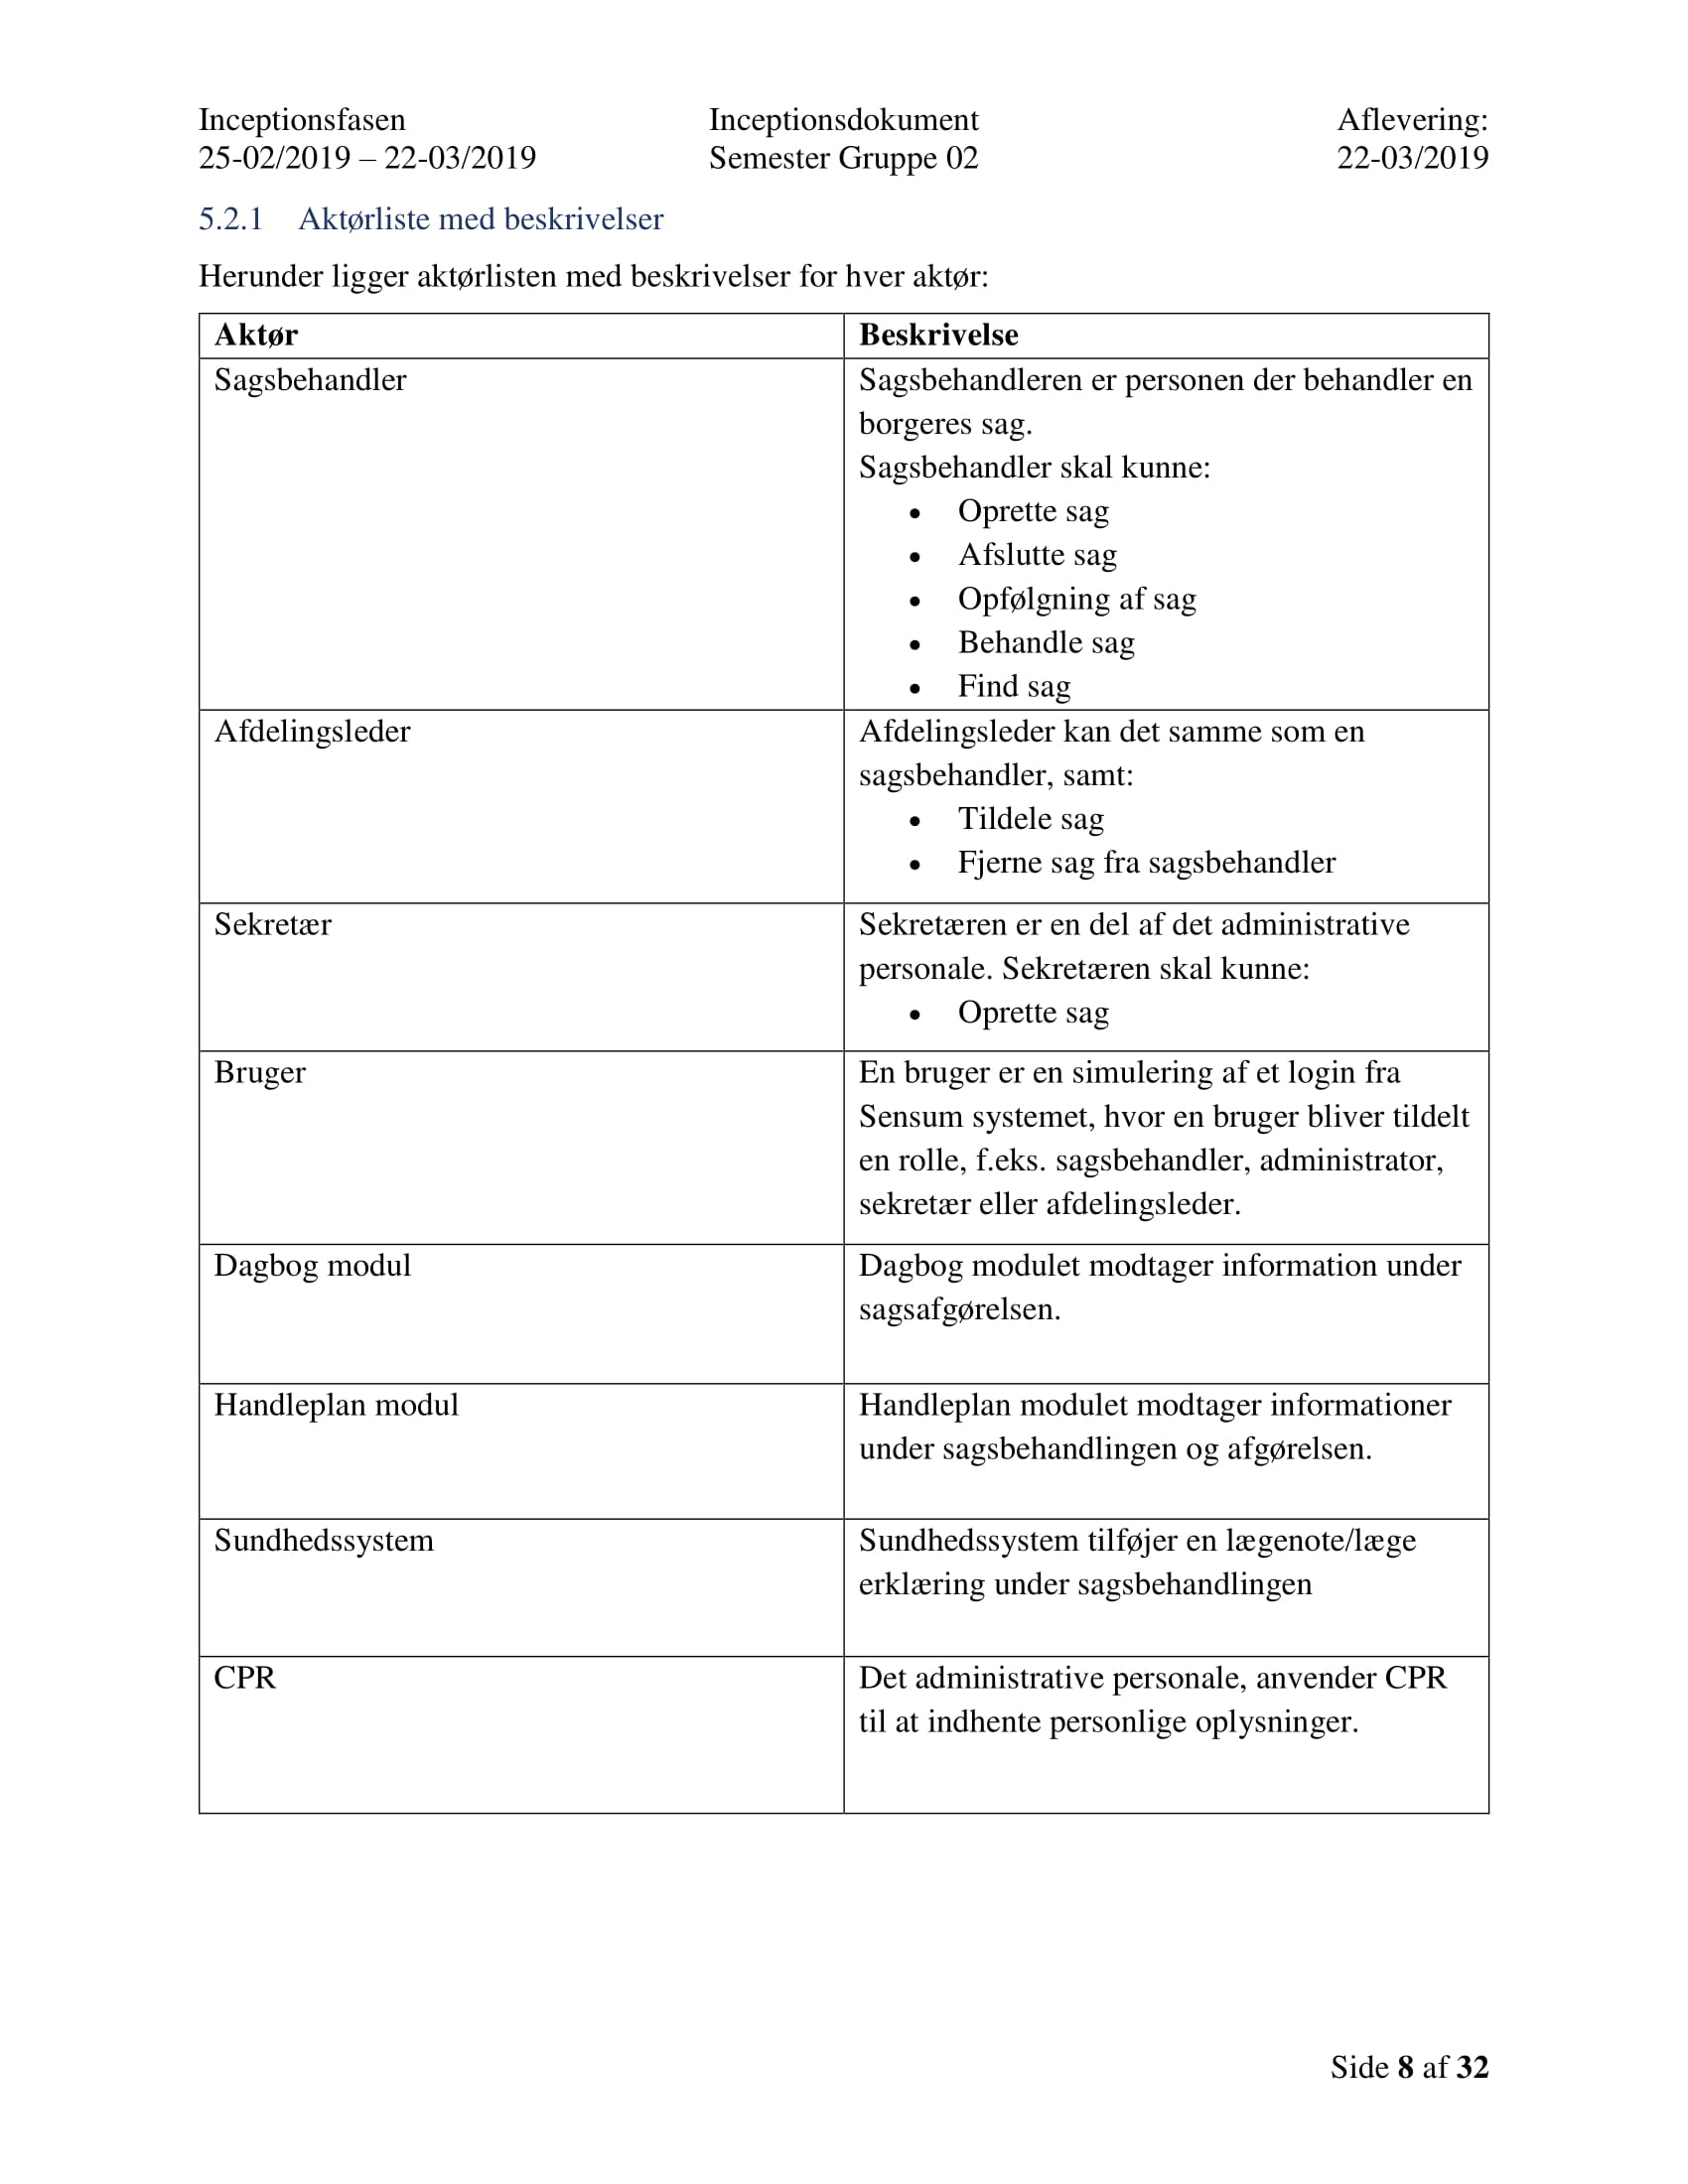
\includegraphics[scale = 0.33]{./PNG/Inceptions/Gruppe 02 + InceptionsDokument-09.jpg} 
\end{figure}

\begin{figure}[hb]
  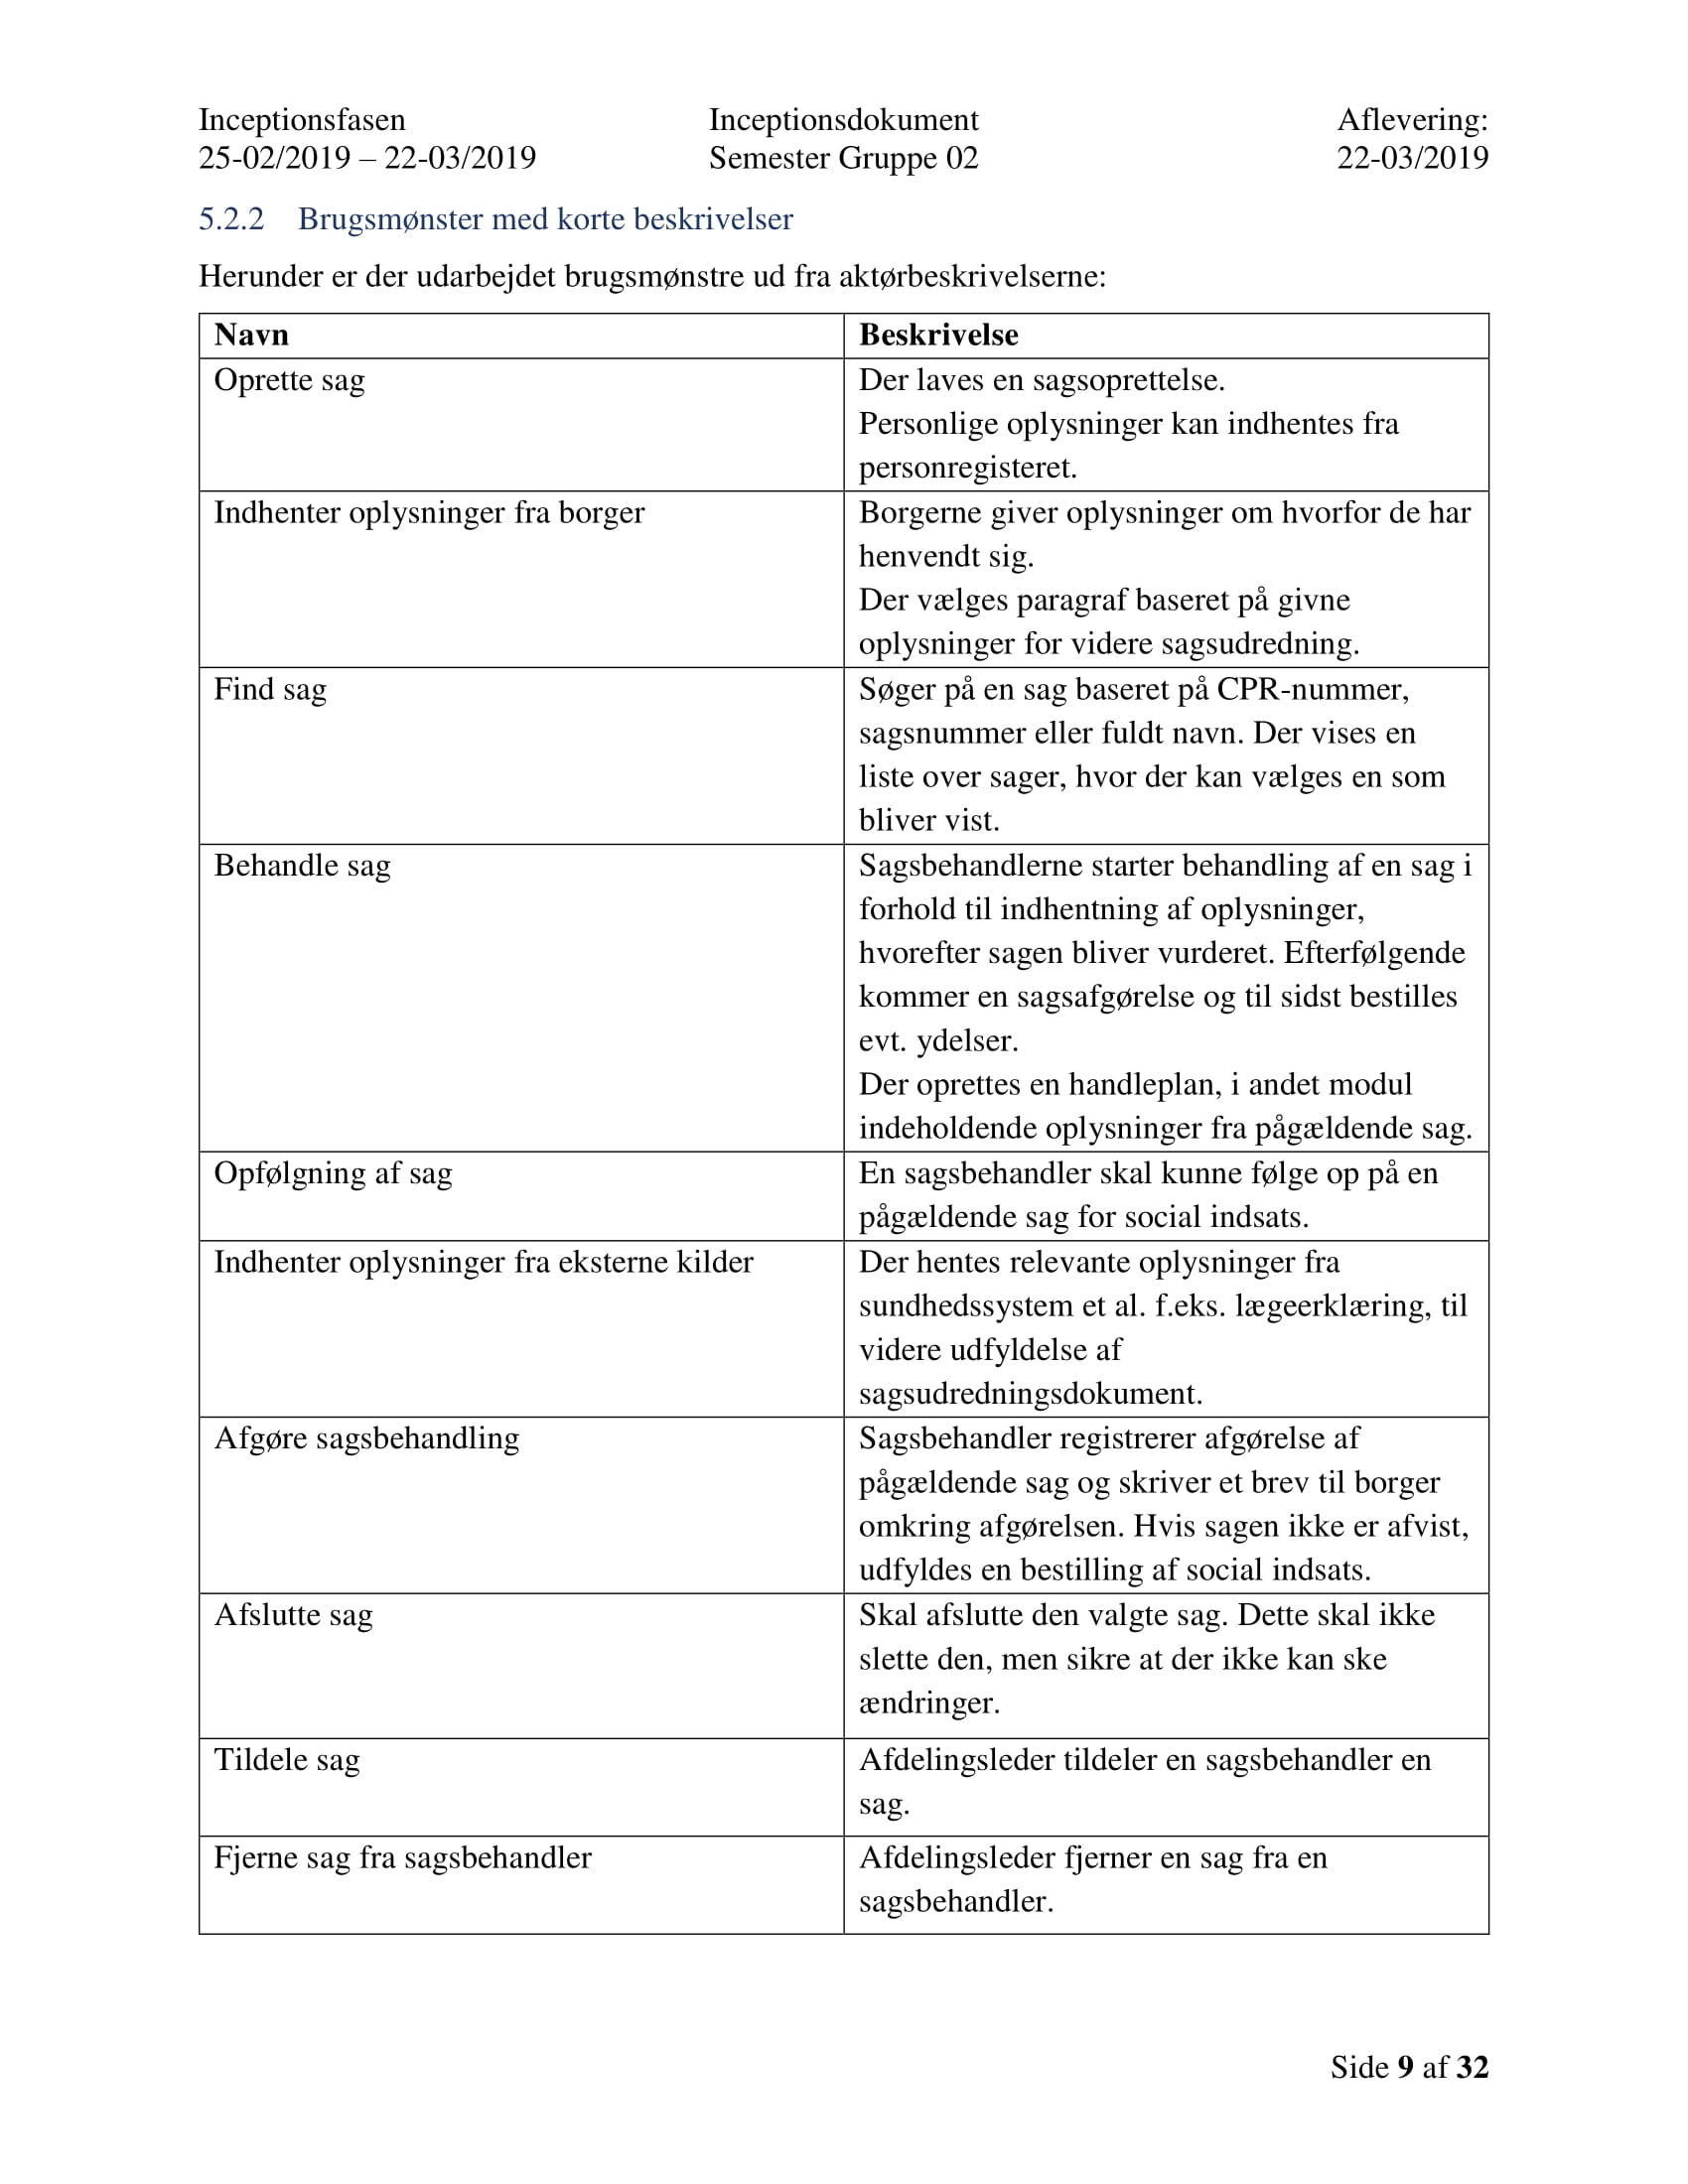
\includegraphics[scale = 0.33]{./PNG/Inceptions/Gruppe 02 + InceptionsDokument-10.jpg} 
\end{figure}

\begin{figure}[hb]
  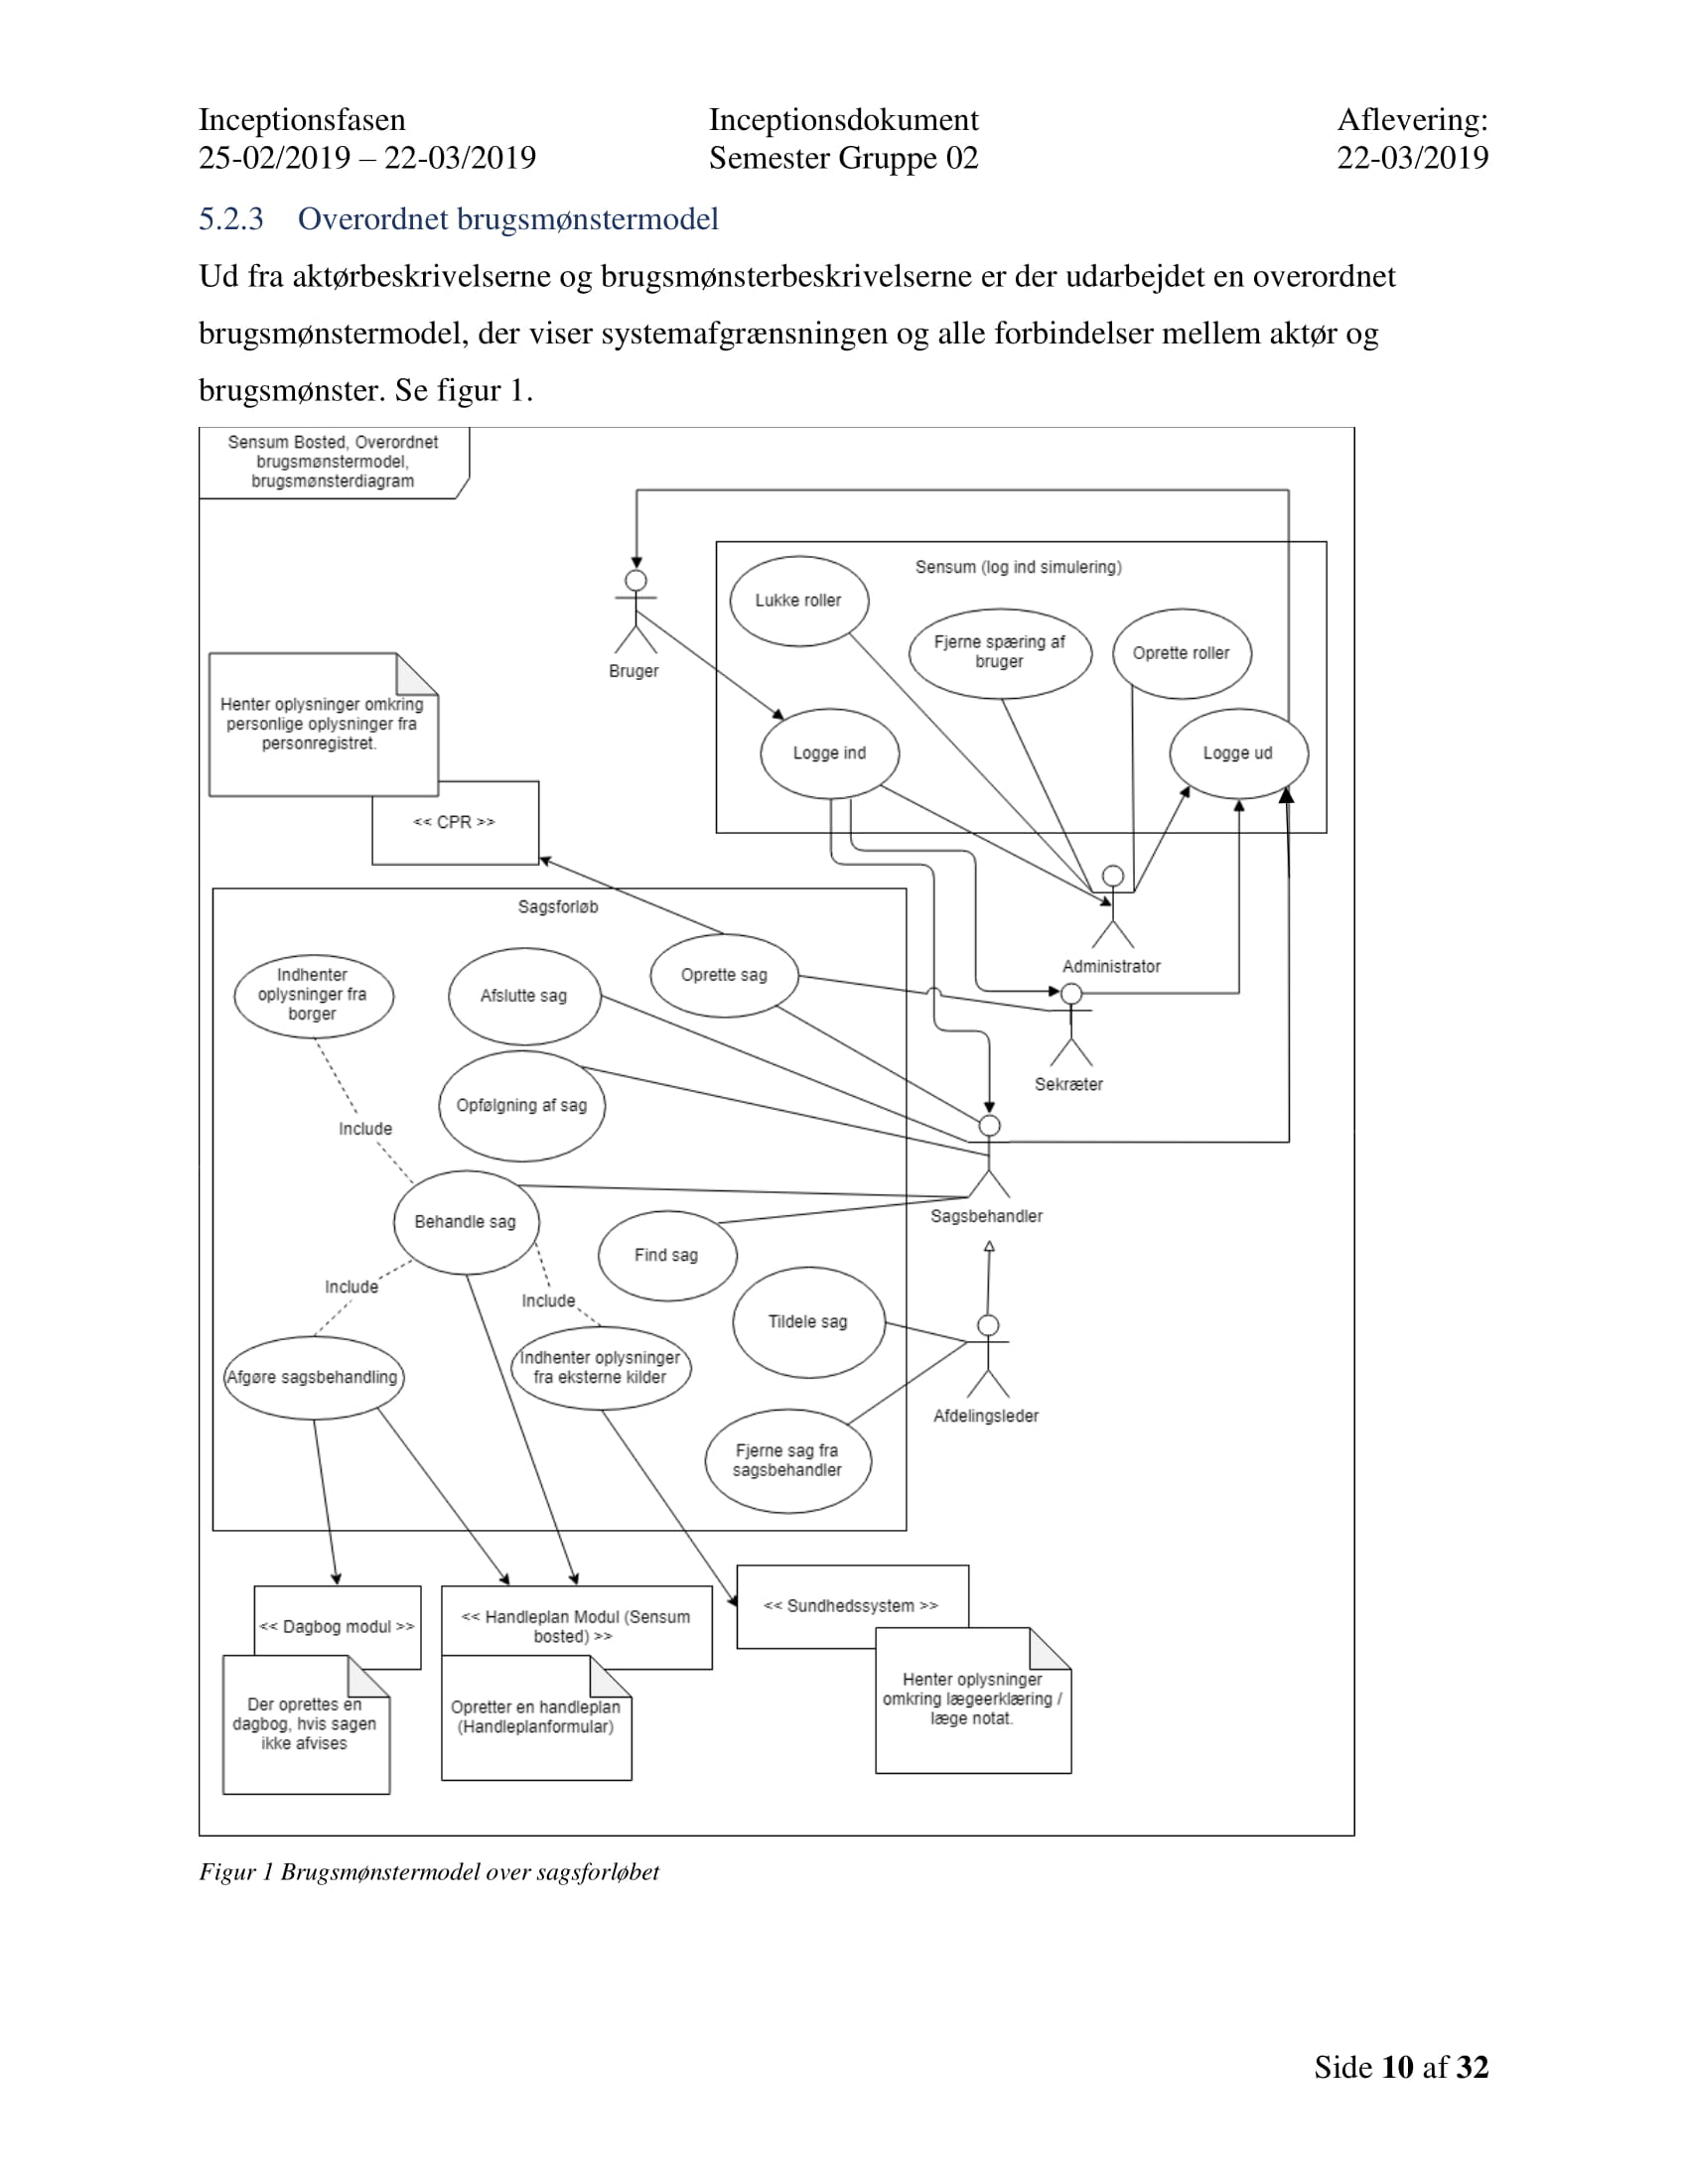
\includegraphics[scale = 0.33]{./PNG/Inceptions/Gruppe 02 + InceptionsDokument-11.jpg} 
\end{figure}

\begin{figure}[hb]
  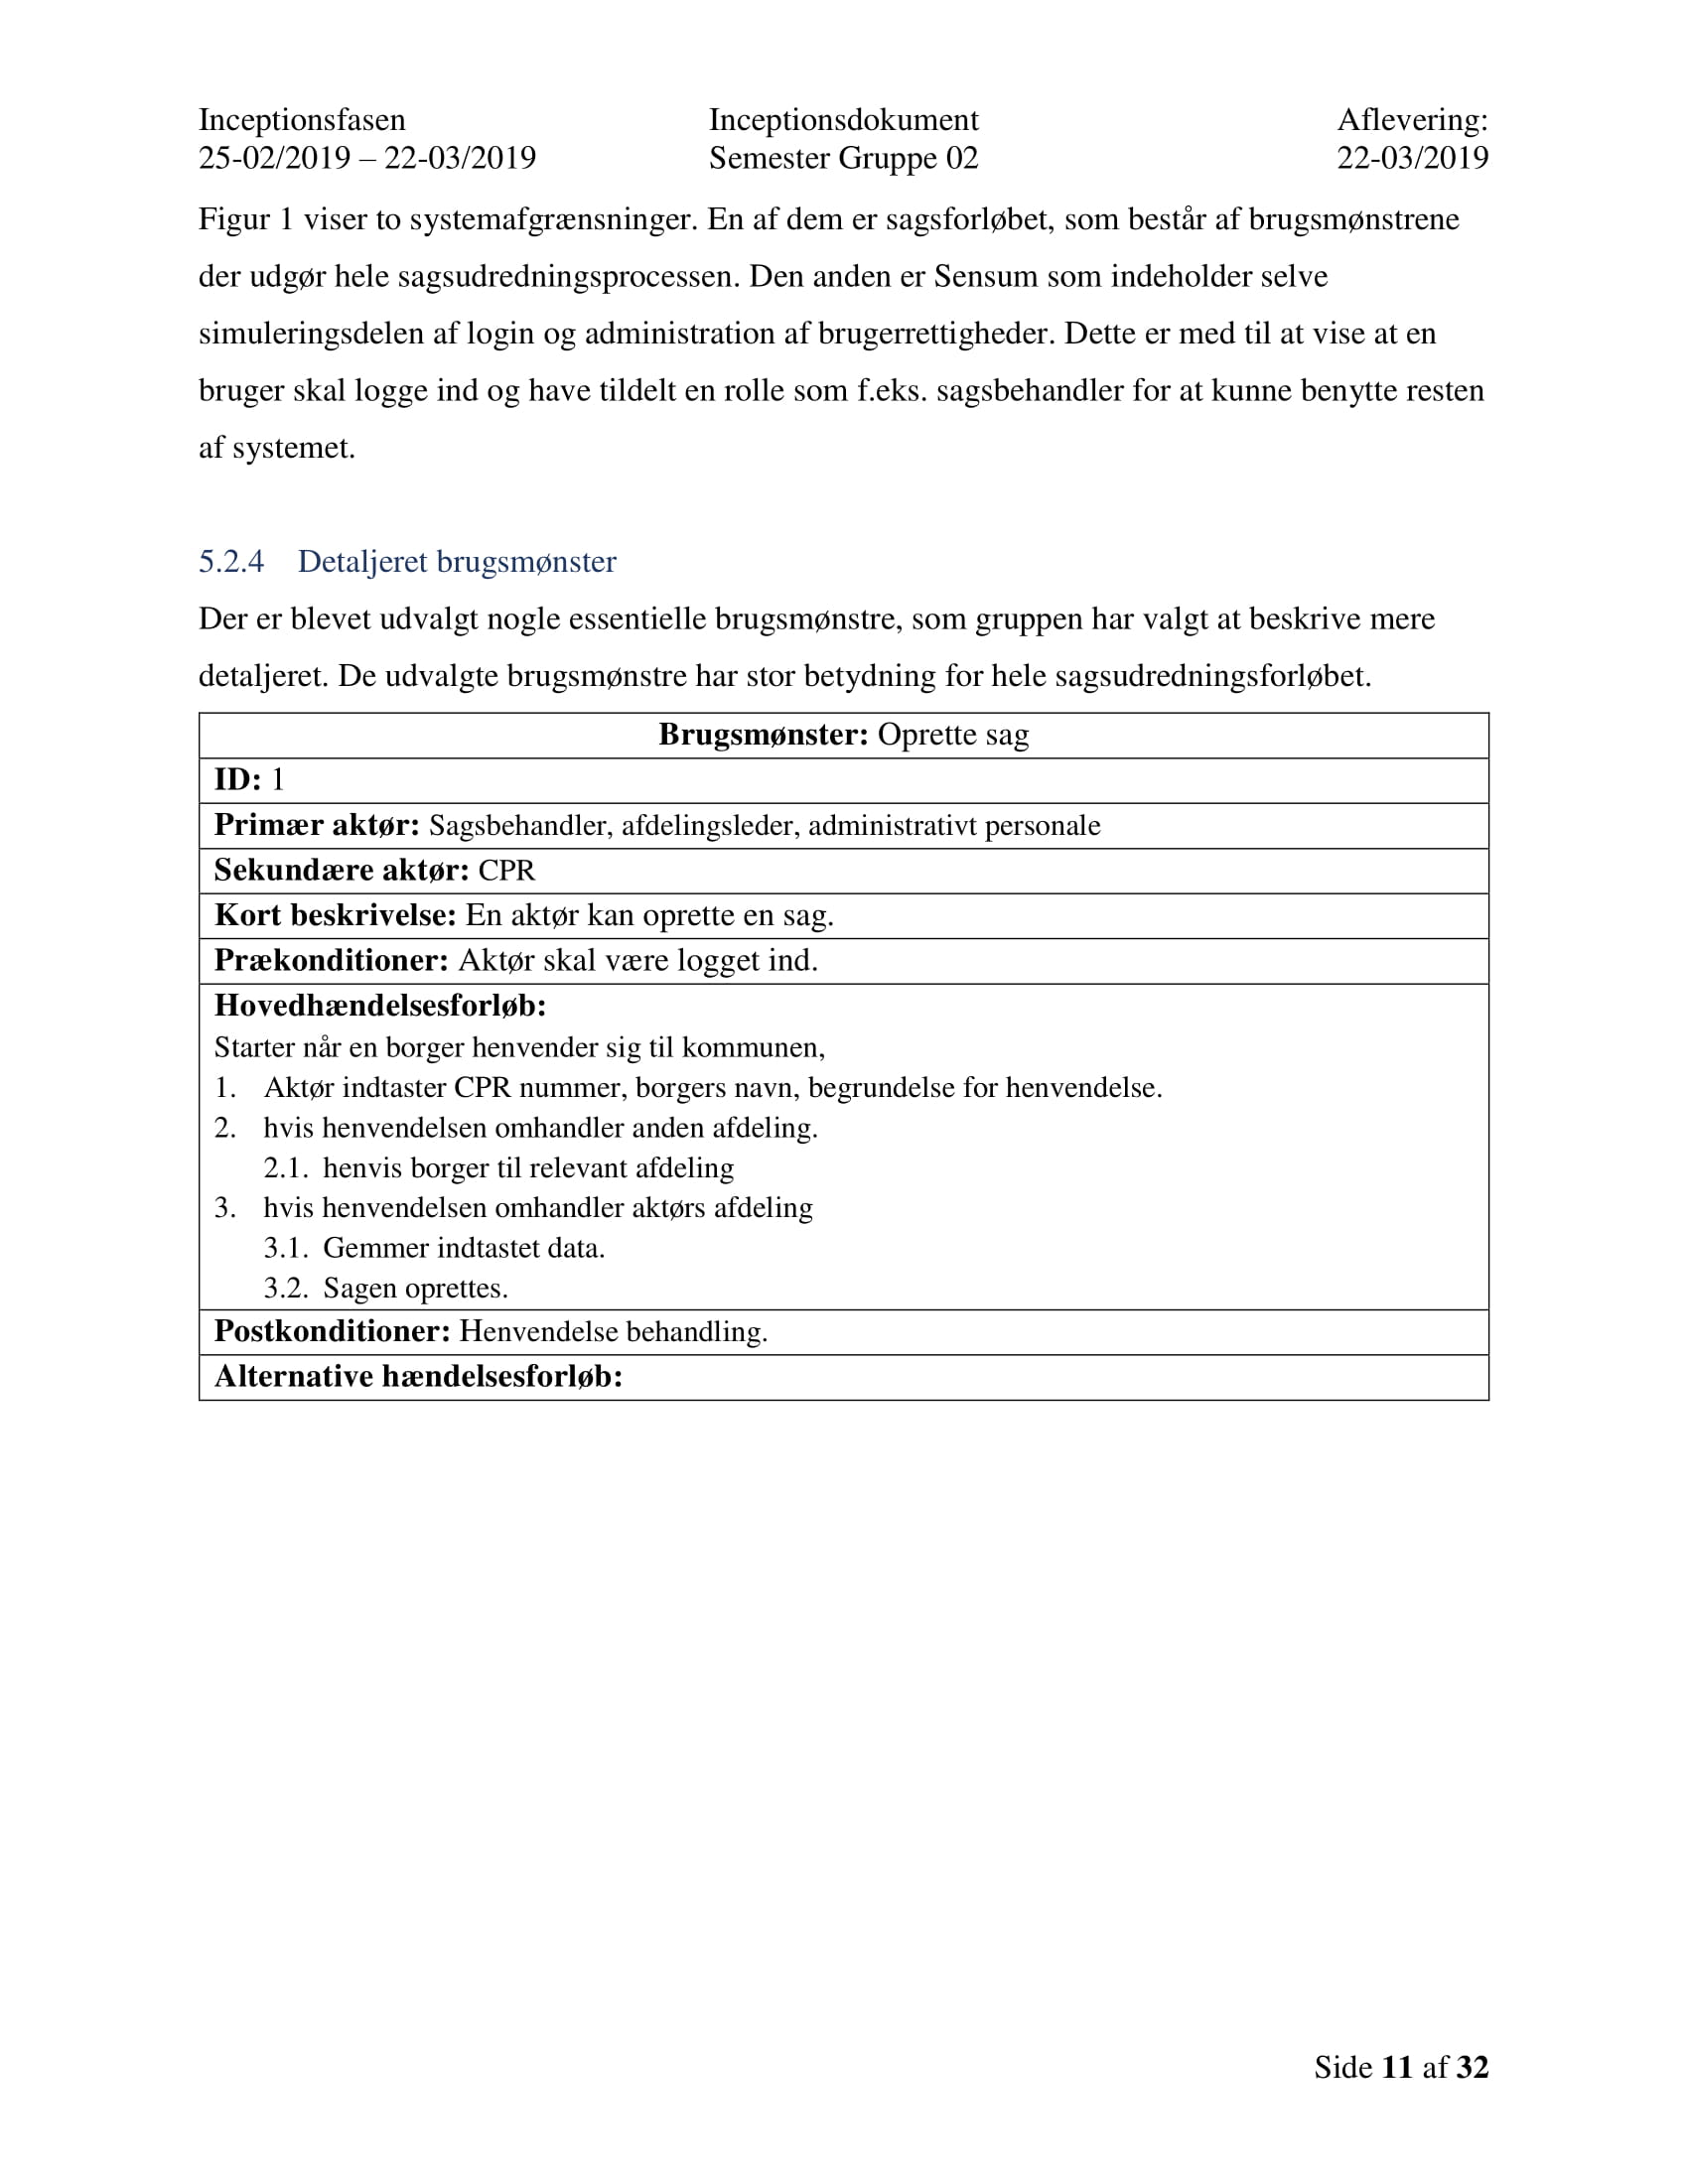
\includegraphics[scale = 0.33]{./PNG/Inceptions/Gruppe 02 + InceptionsDokument-12.jpg} 
\end{figure}

\begin{figure}[hb]
  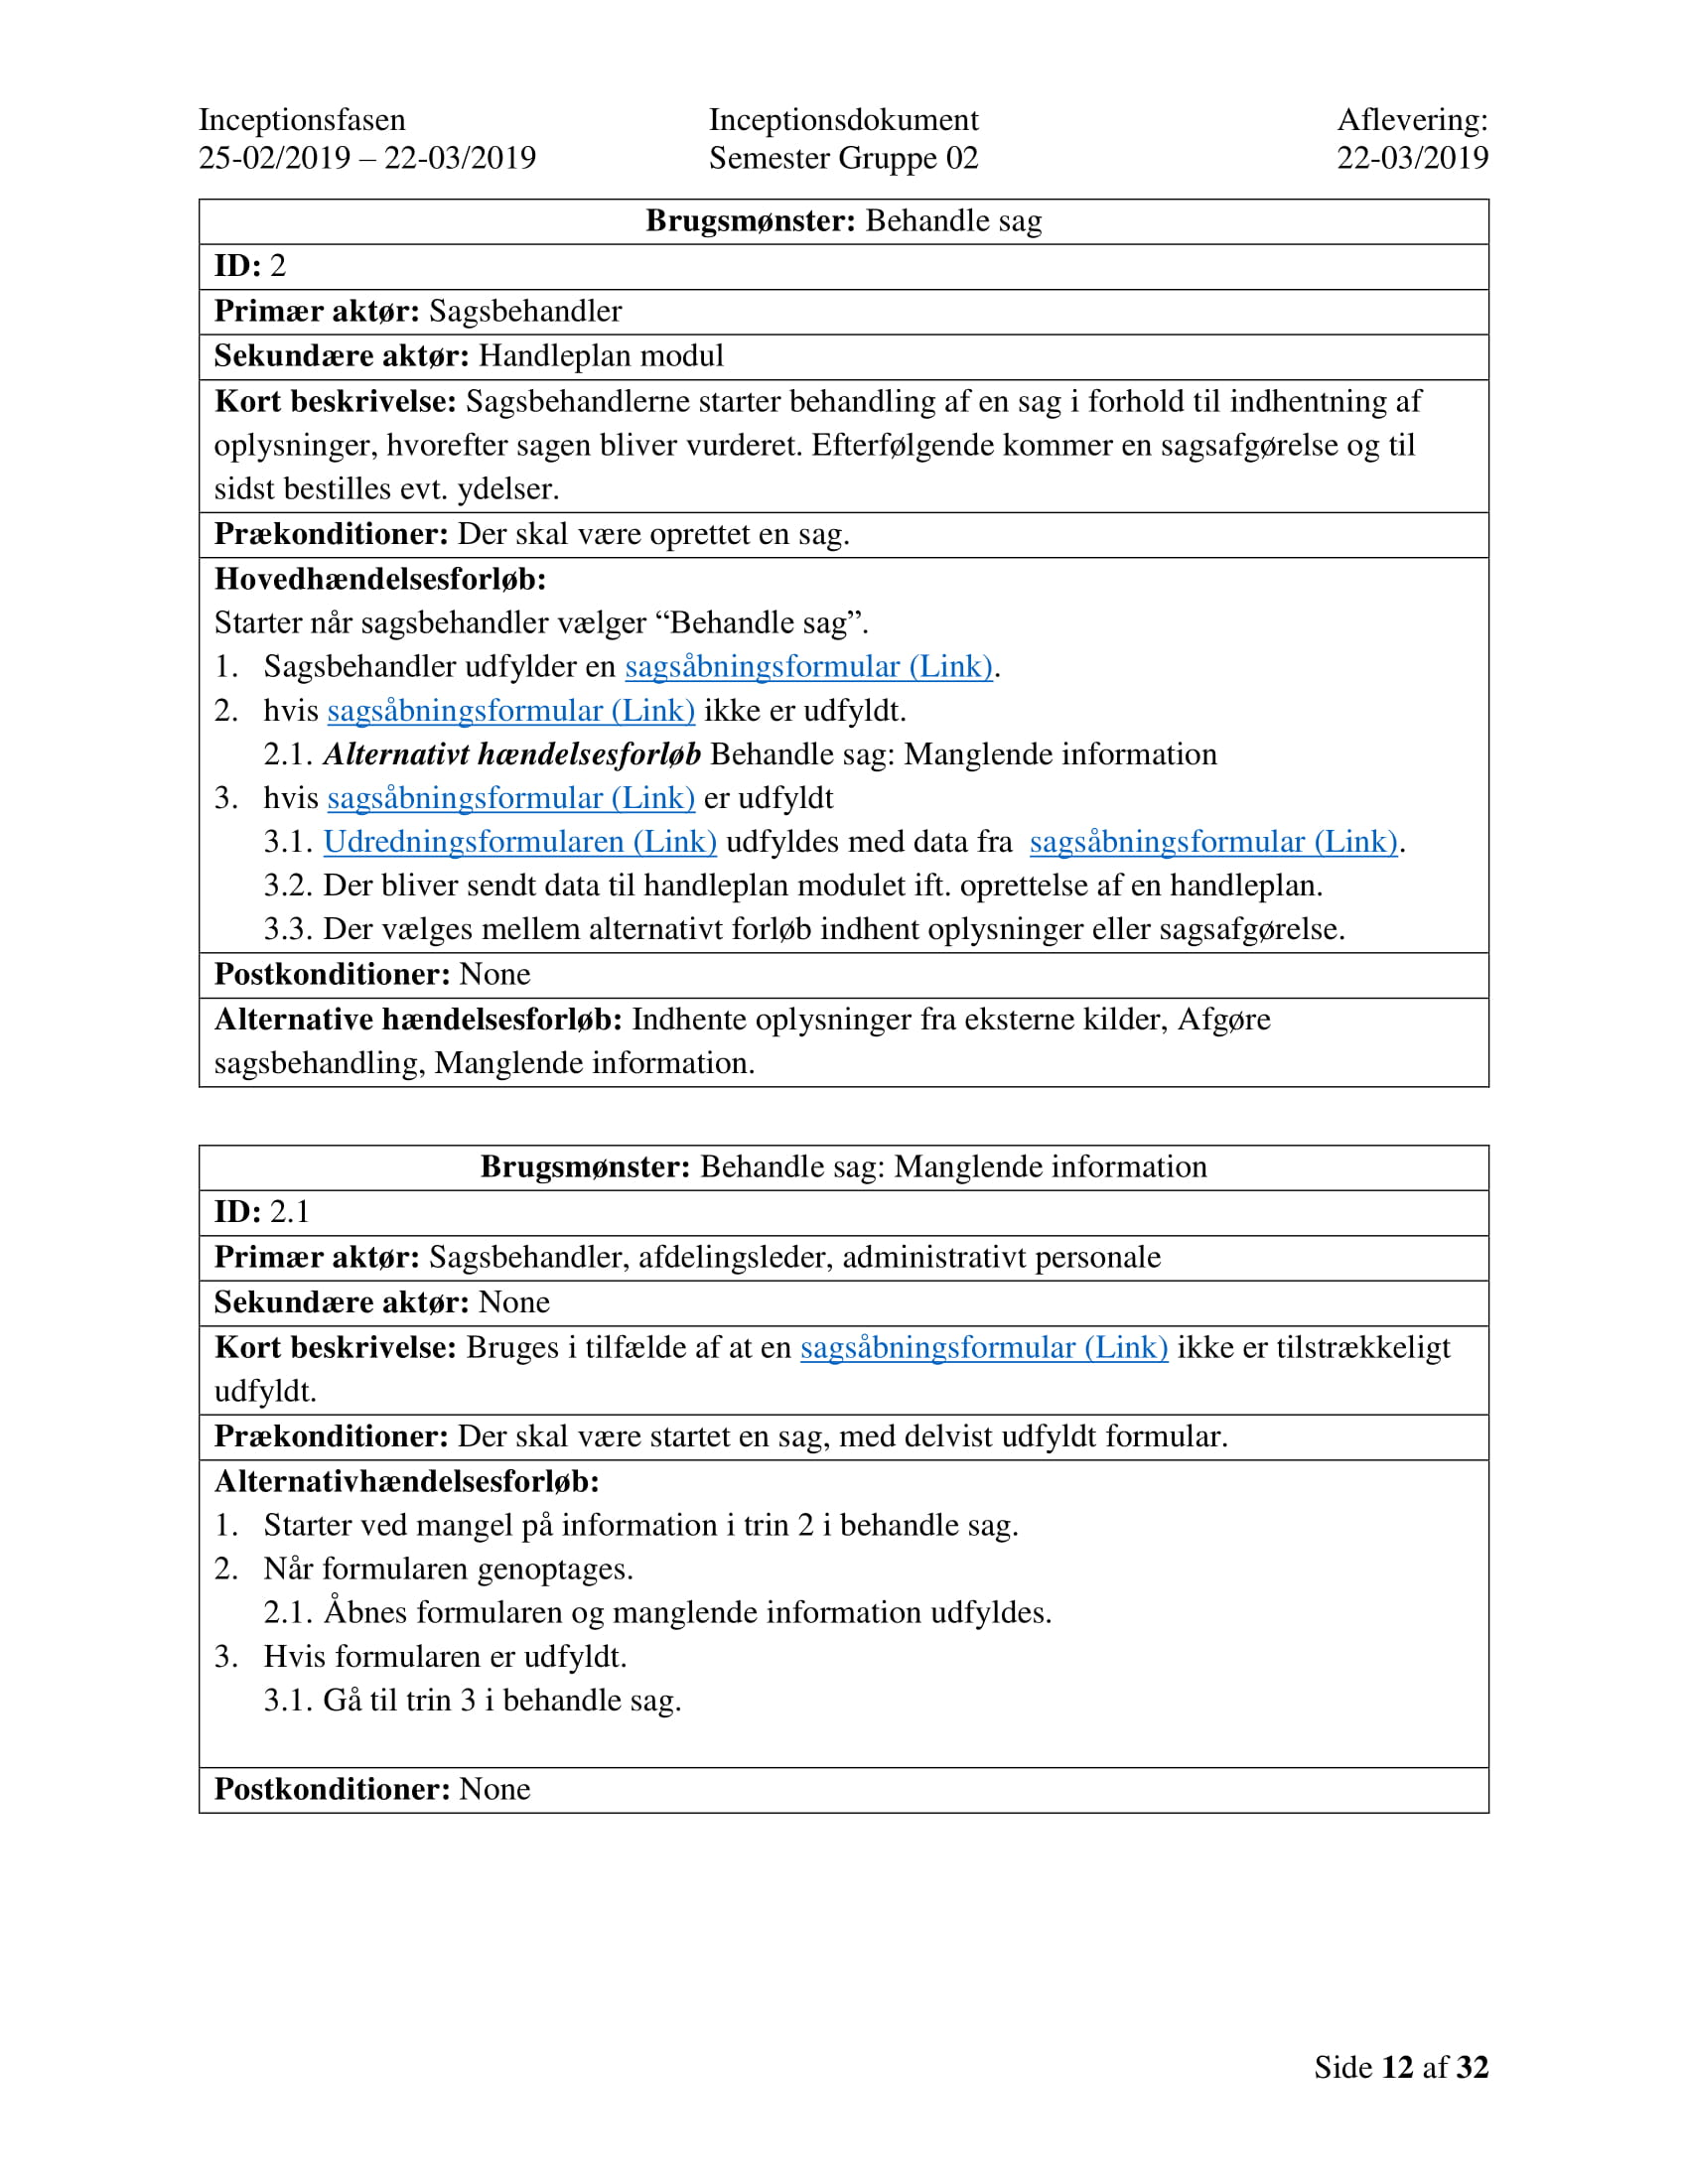
\includegraphics[scale = 0.33]{./PNG/Inceptions/Gruppe 02 + InceptionsDokument-13.jpg} 
\end{figure}

\begin{figure}[hb]
  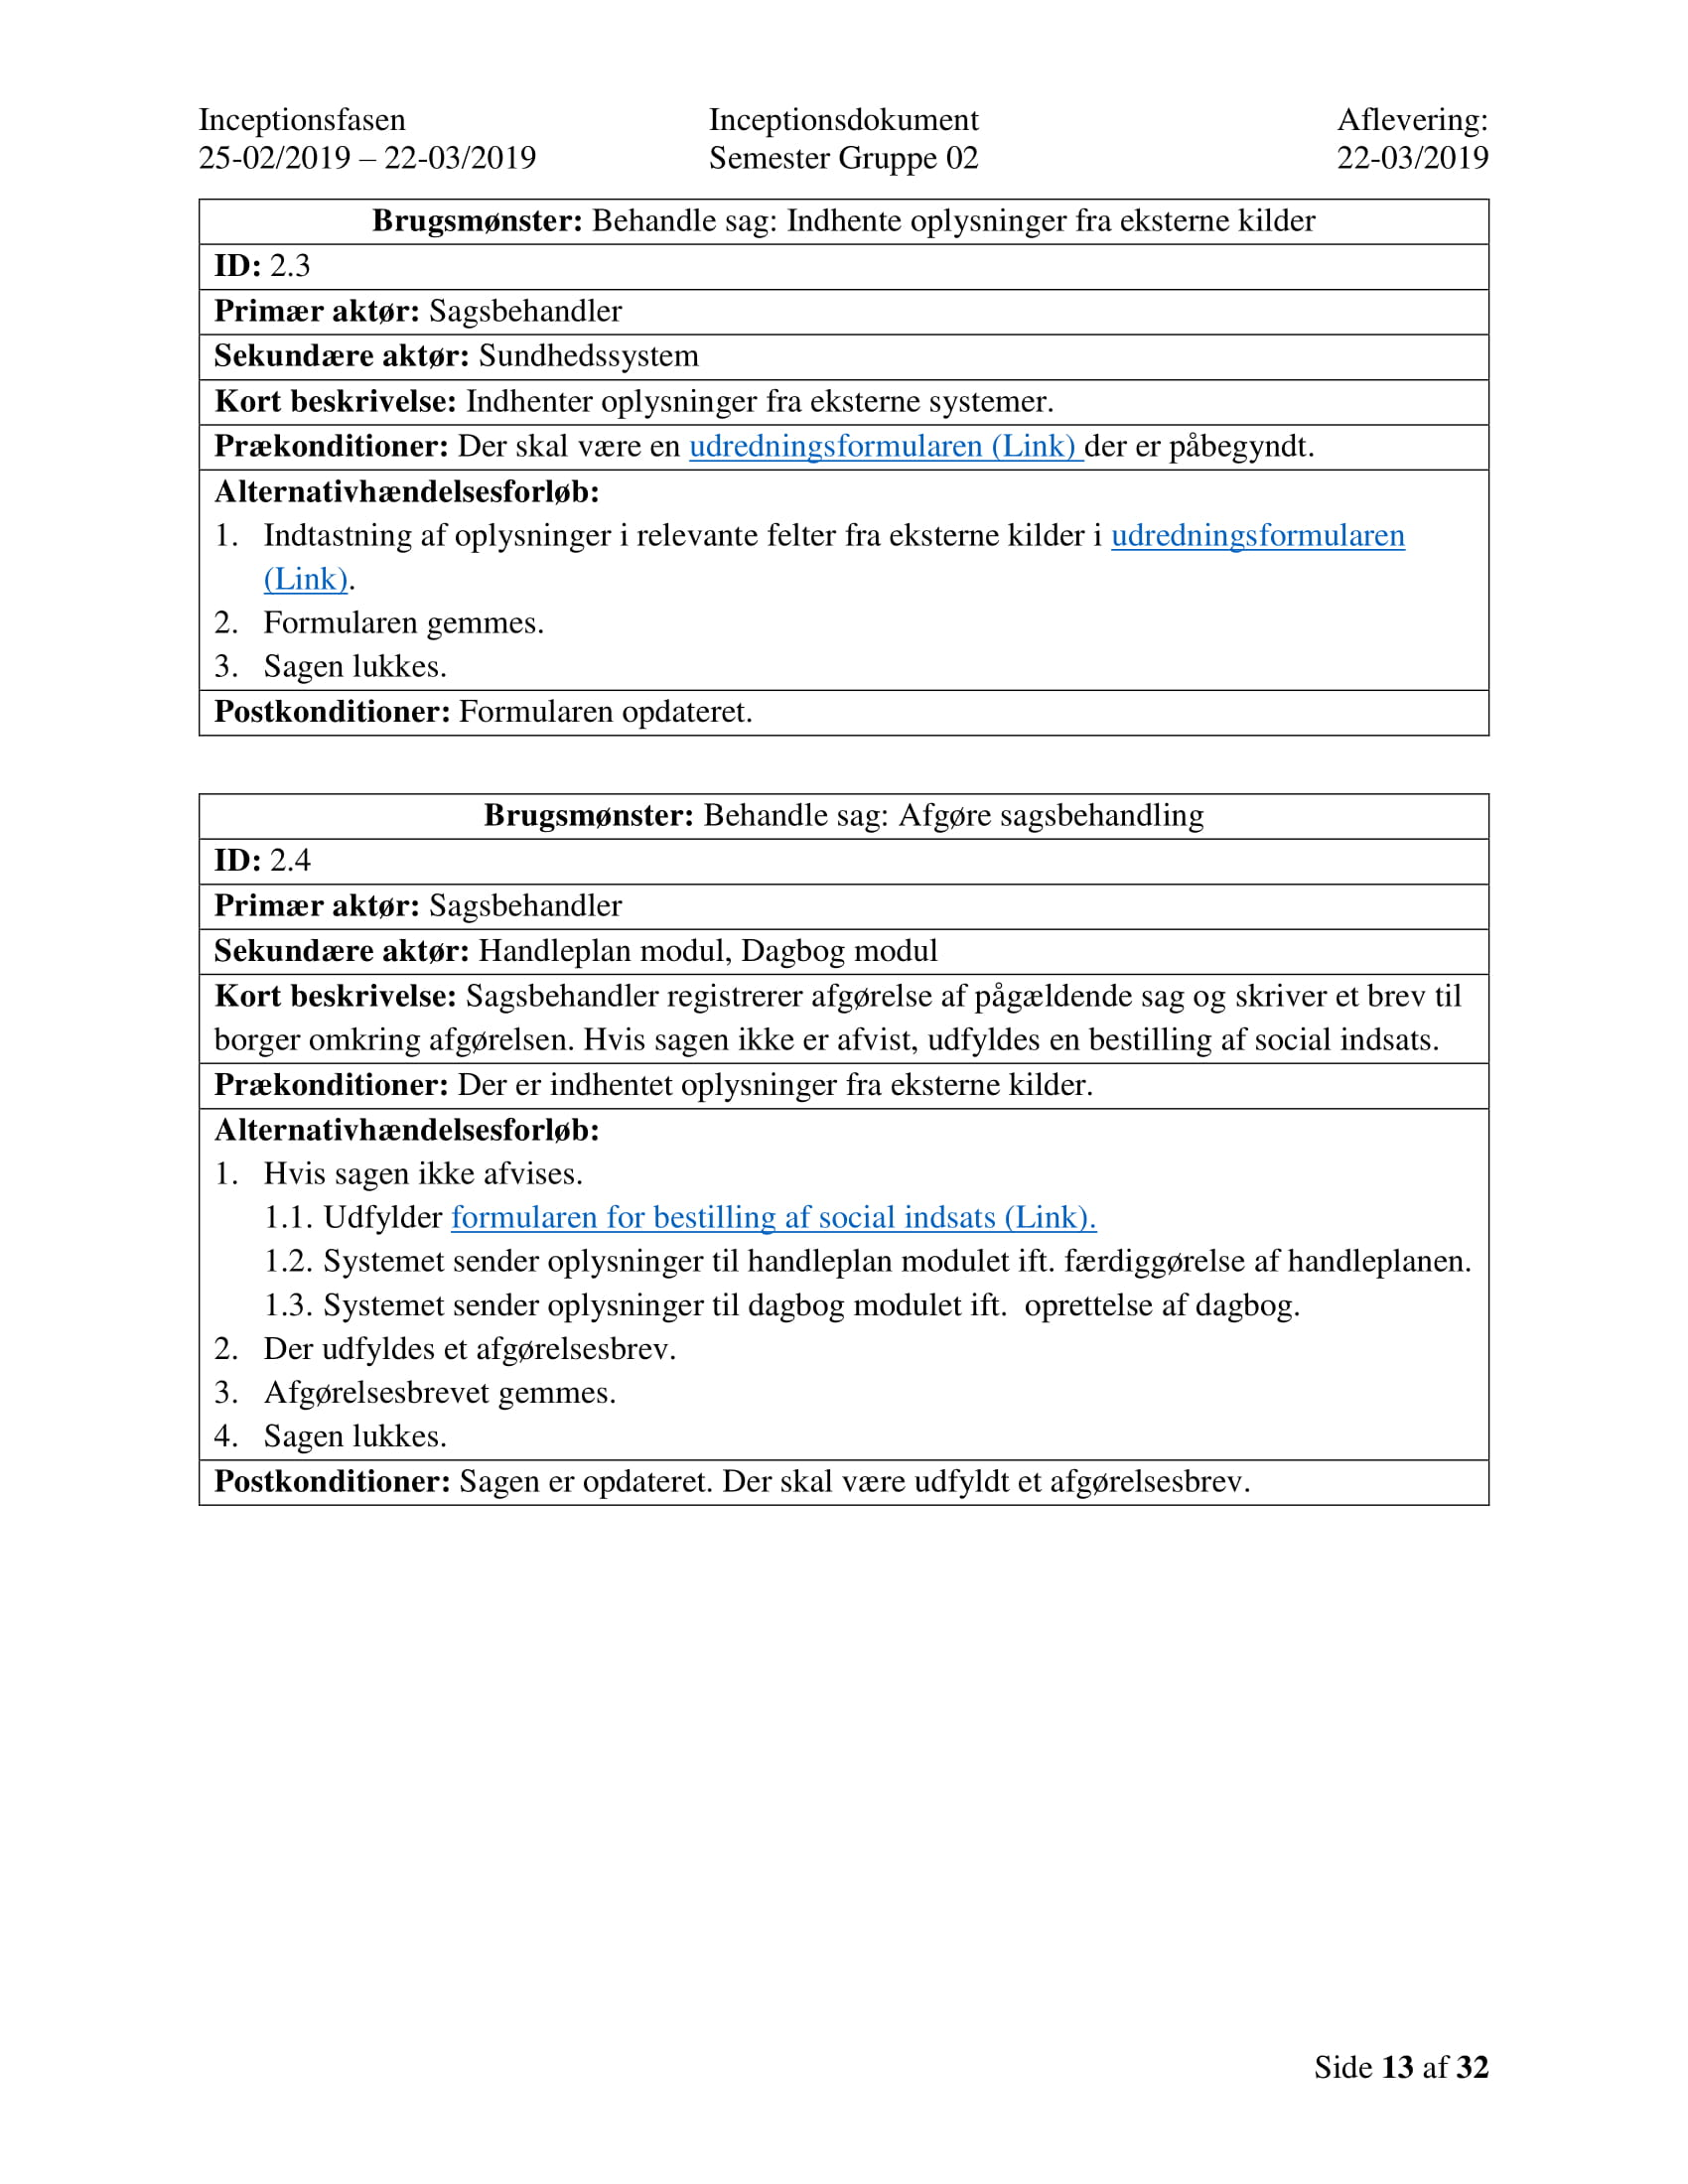
\includegraphics[scale = 0.33]{./PNG/Inceptions/Gruppe 02 + InceptionsDokument-14.jpg} 
\end{figure}

\begin{figure}[hb]
  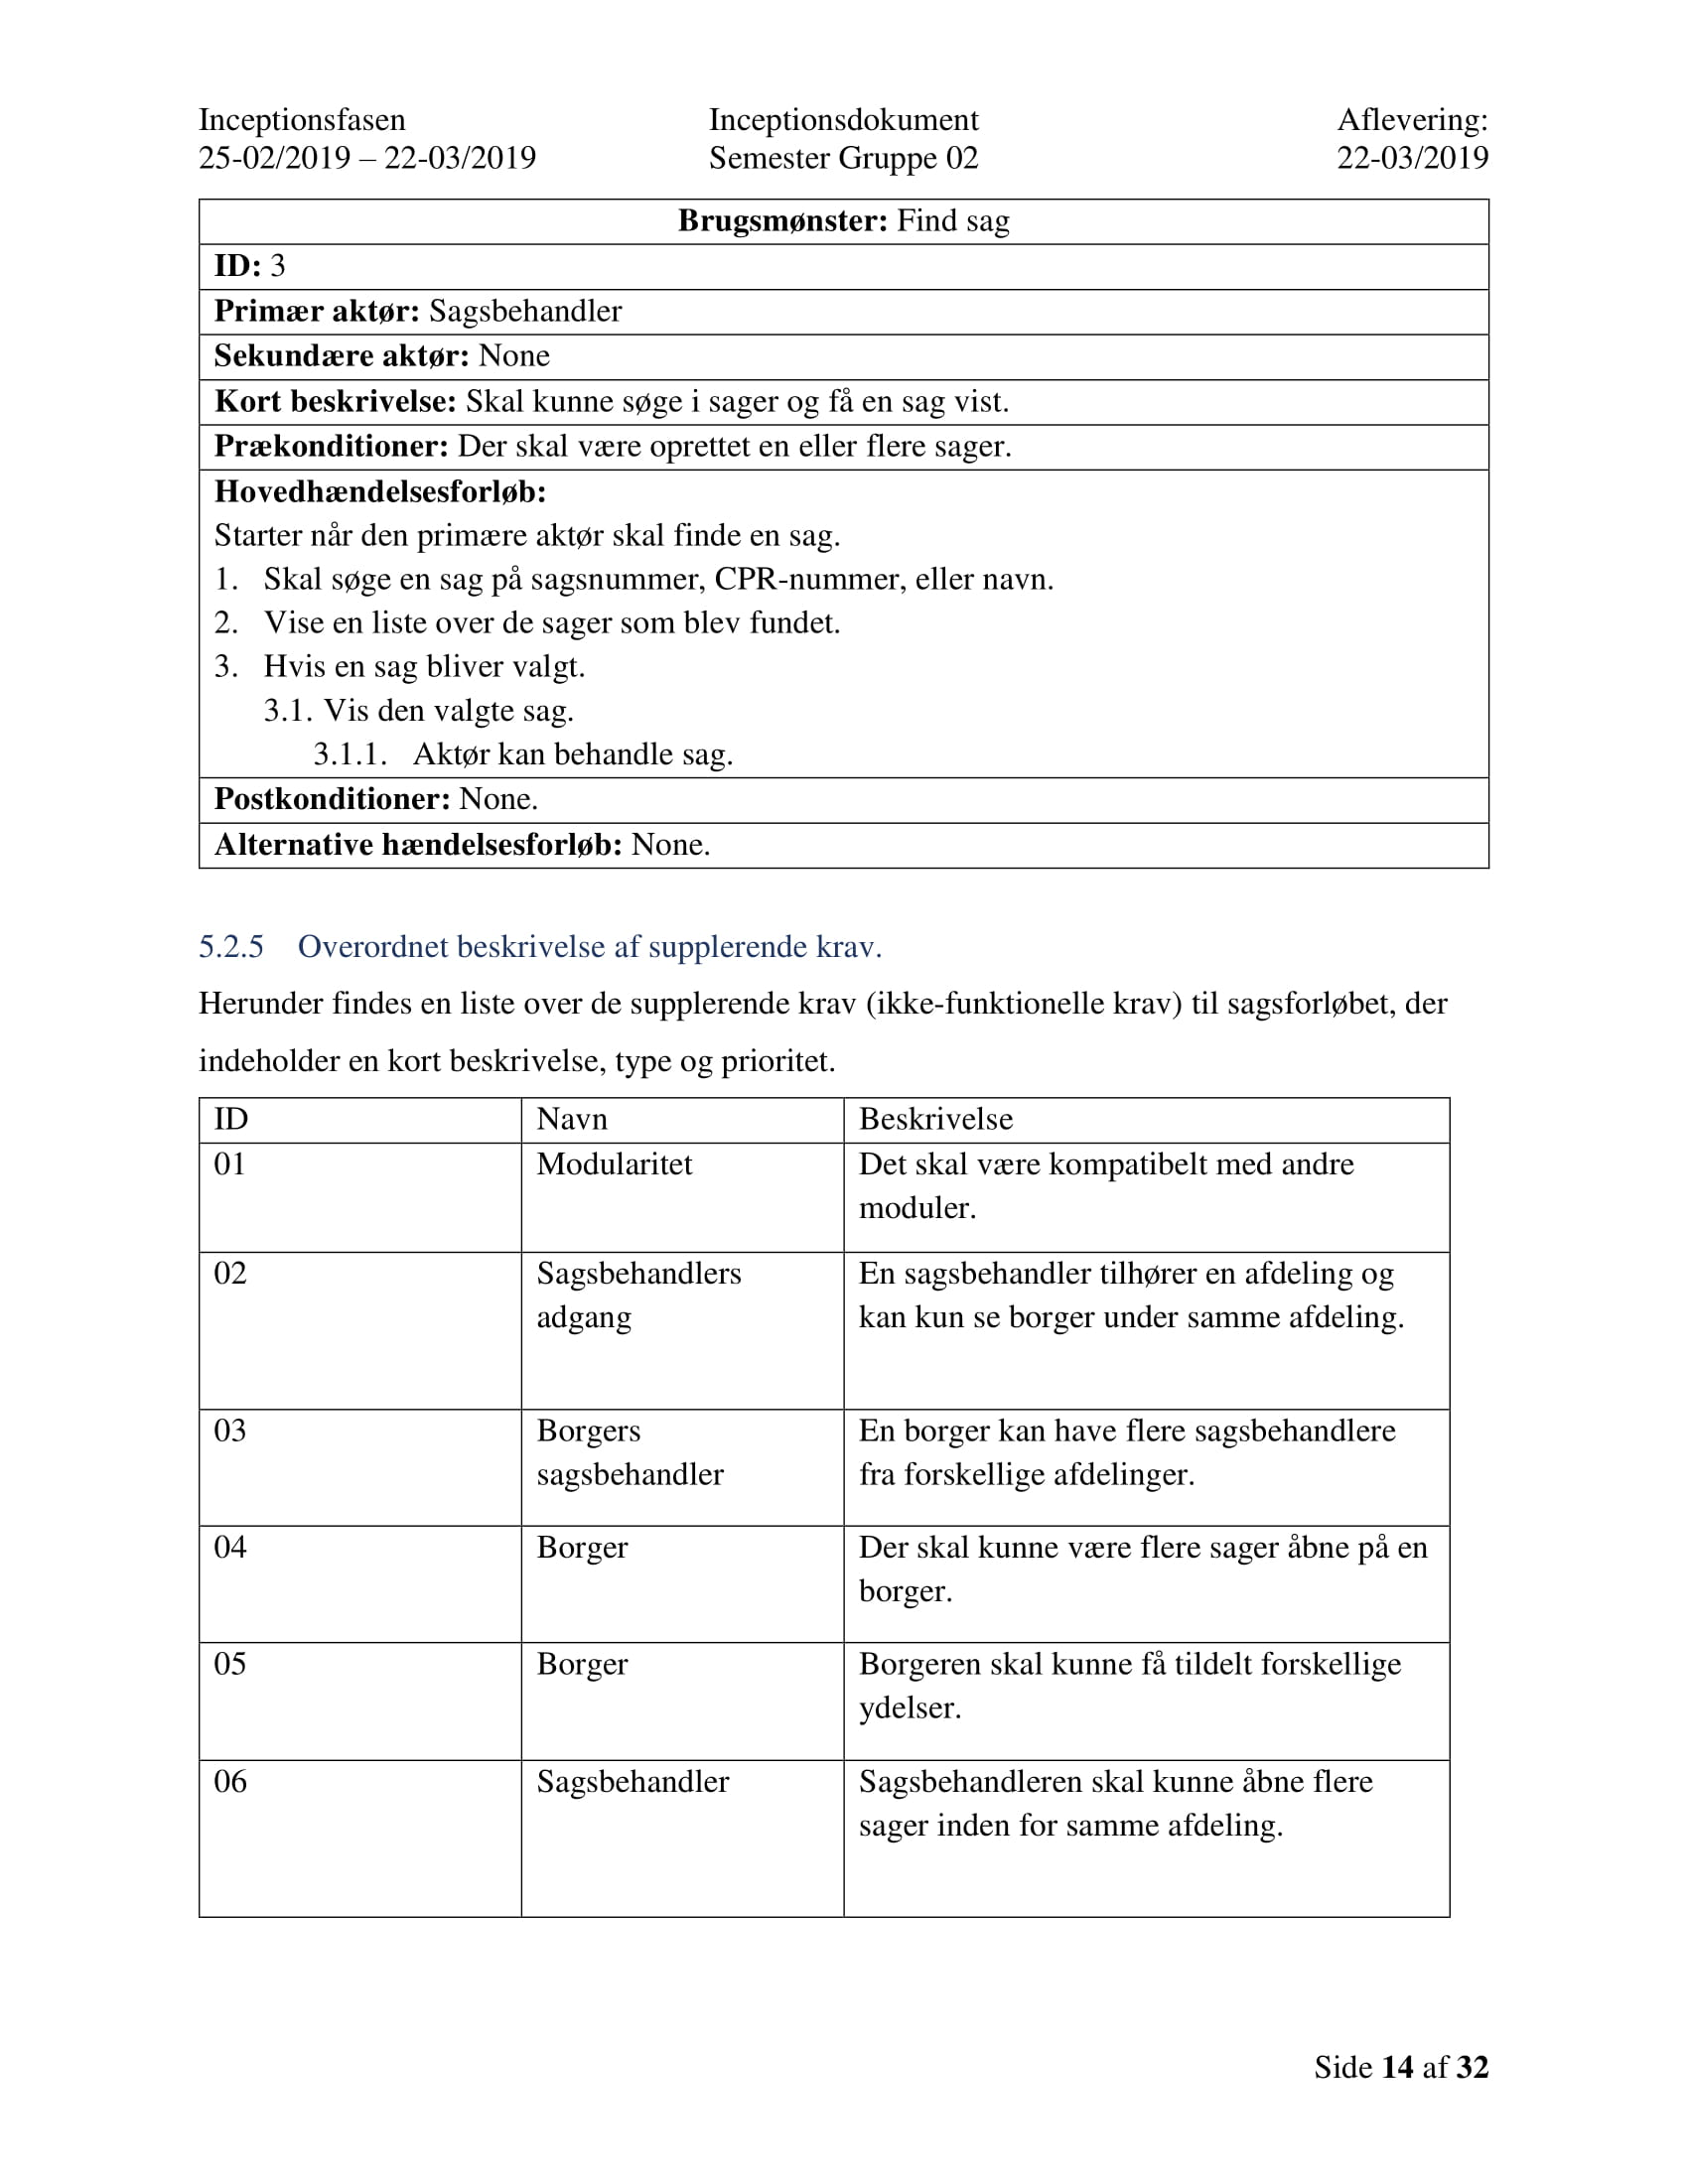
\includegraphics[scale = 0.33]{./PNG/Inceptions/Gruppe 02 + InceptionsDokument-15.jpg} 
\end{figure}

\begin{figure}[hb]
  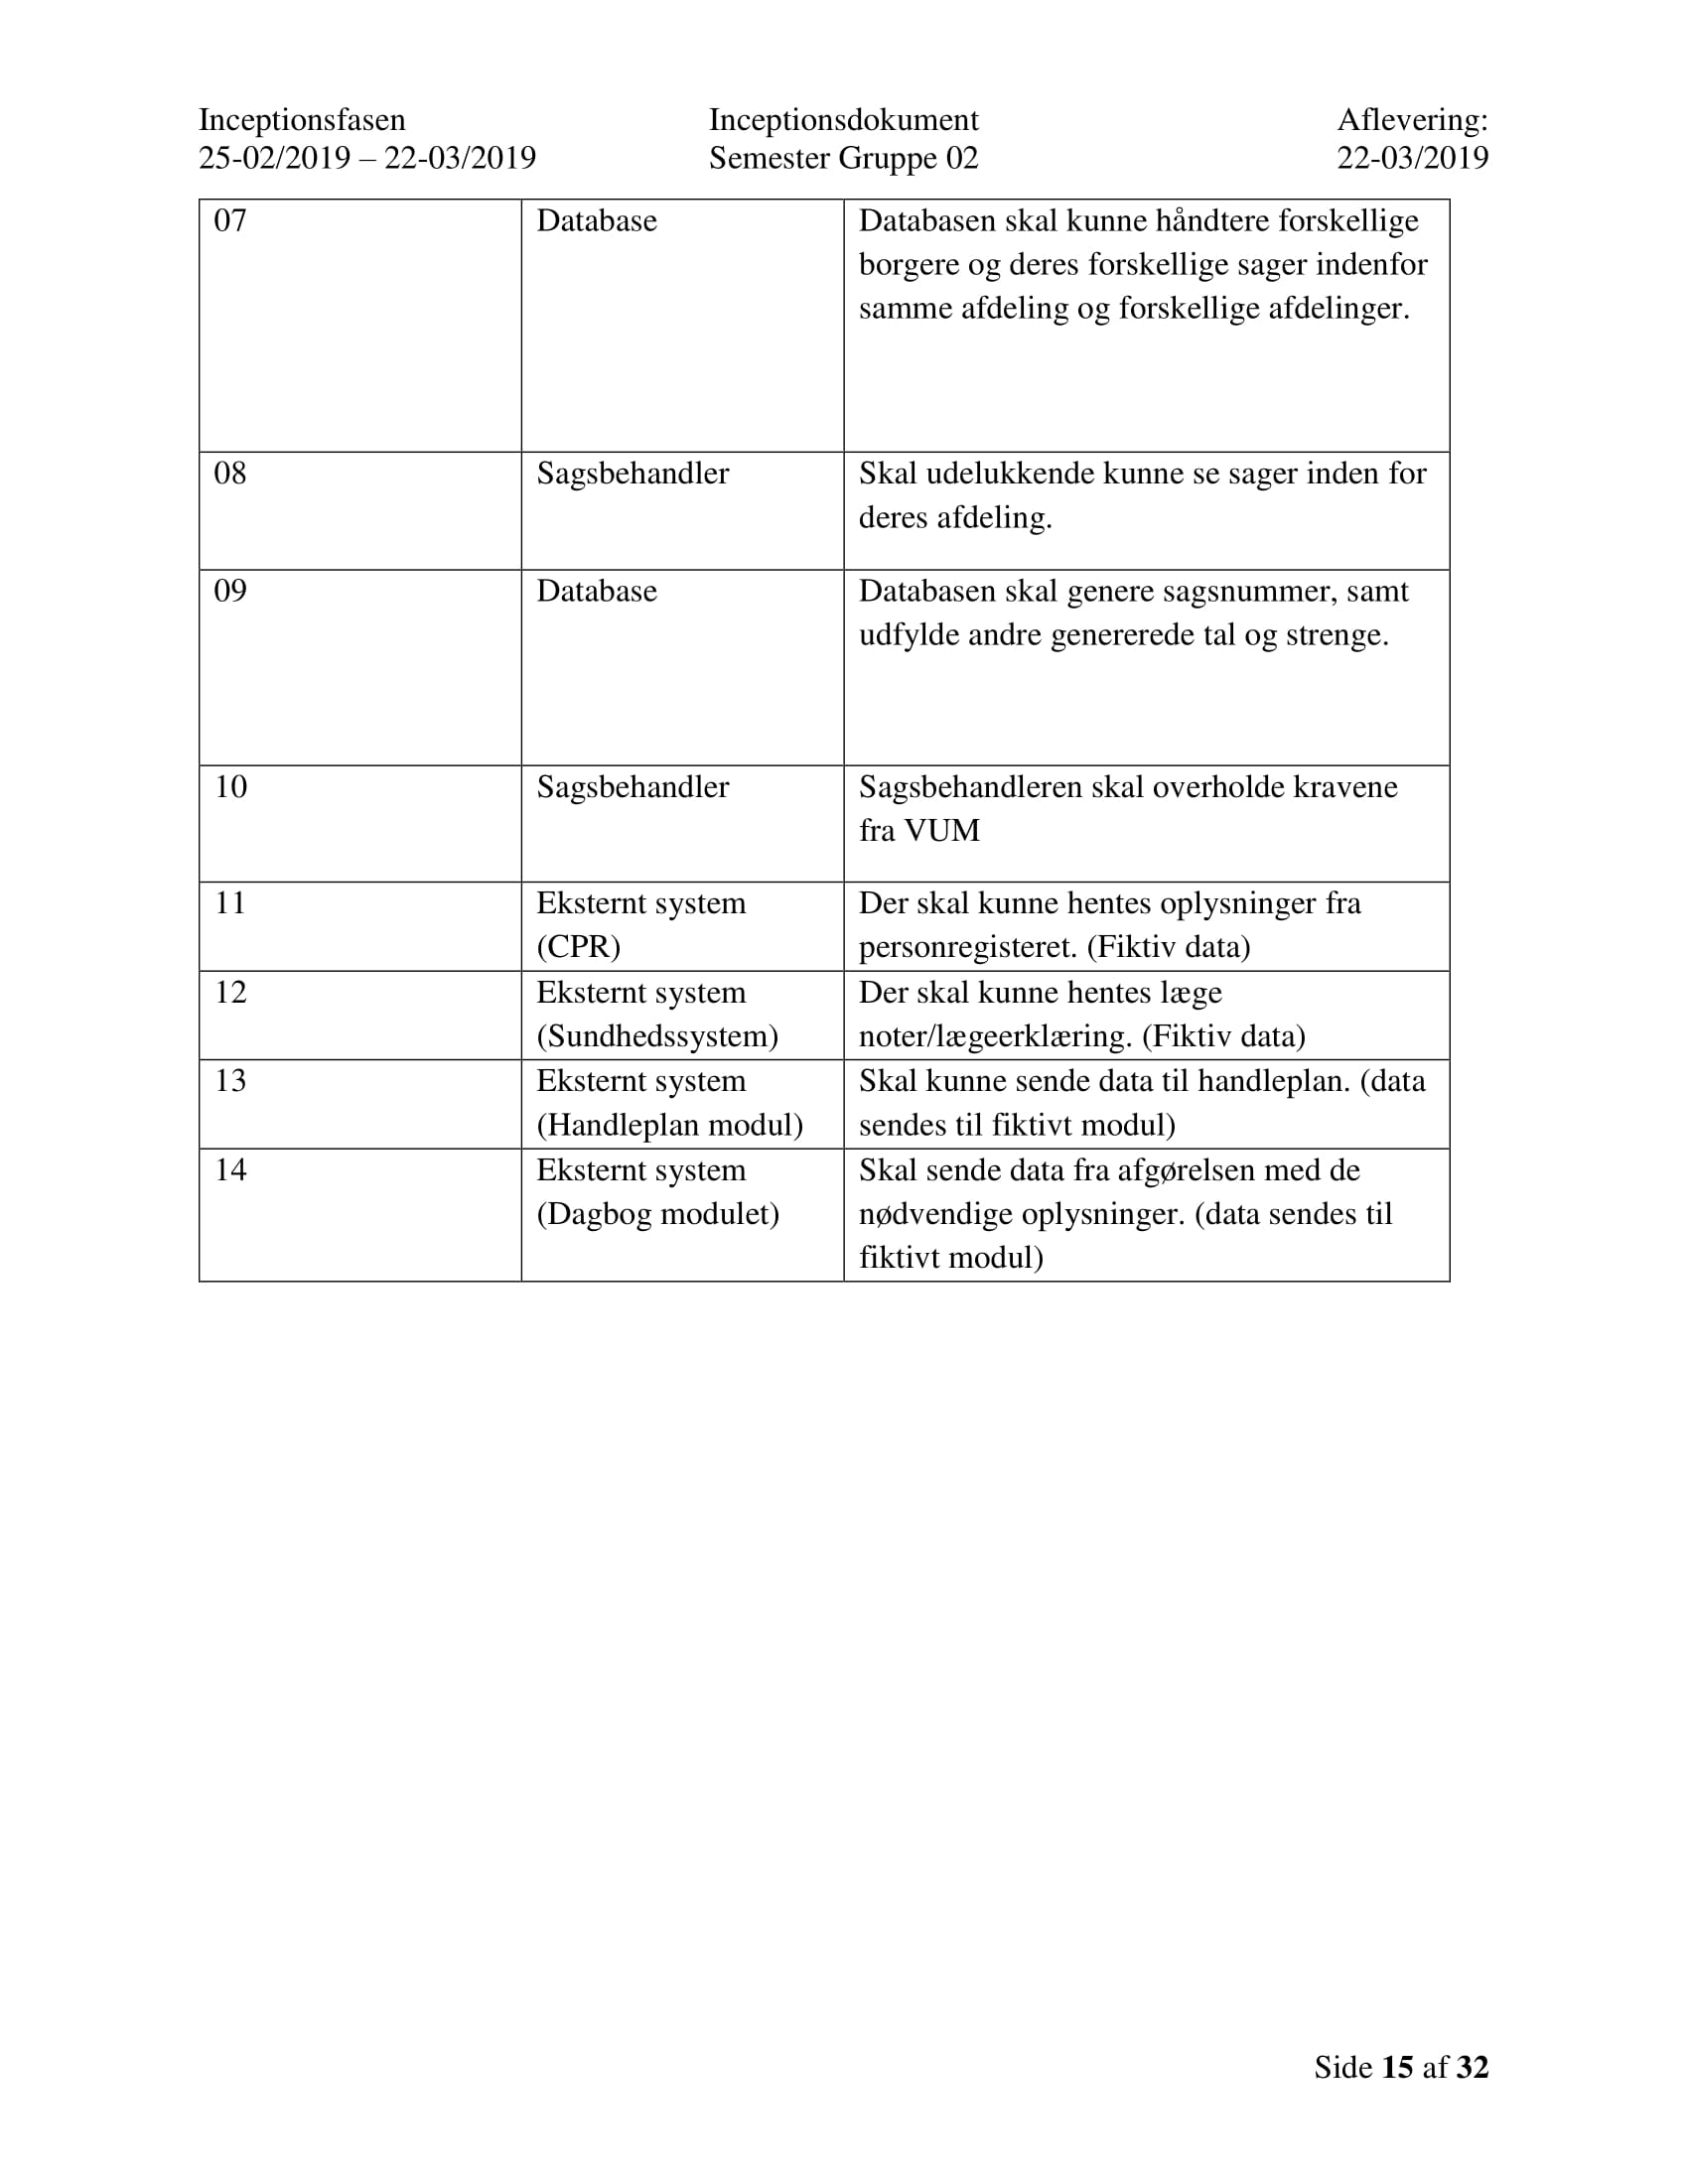
\includegraphics[scale = 0.33]{./PNG/Inceptions/Gruppe 02 + InceptionsDokument-16.jpg} 
\end{figure}

\begin{figure}[hb]
  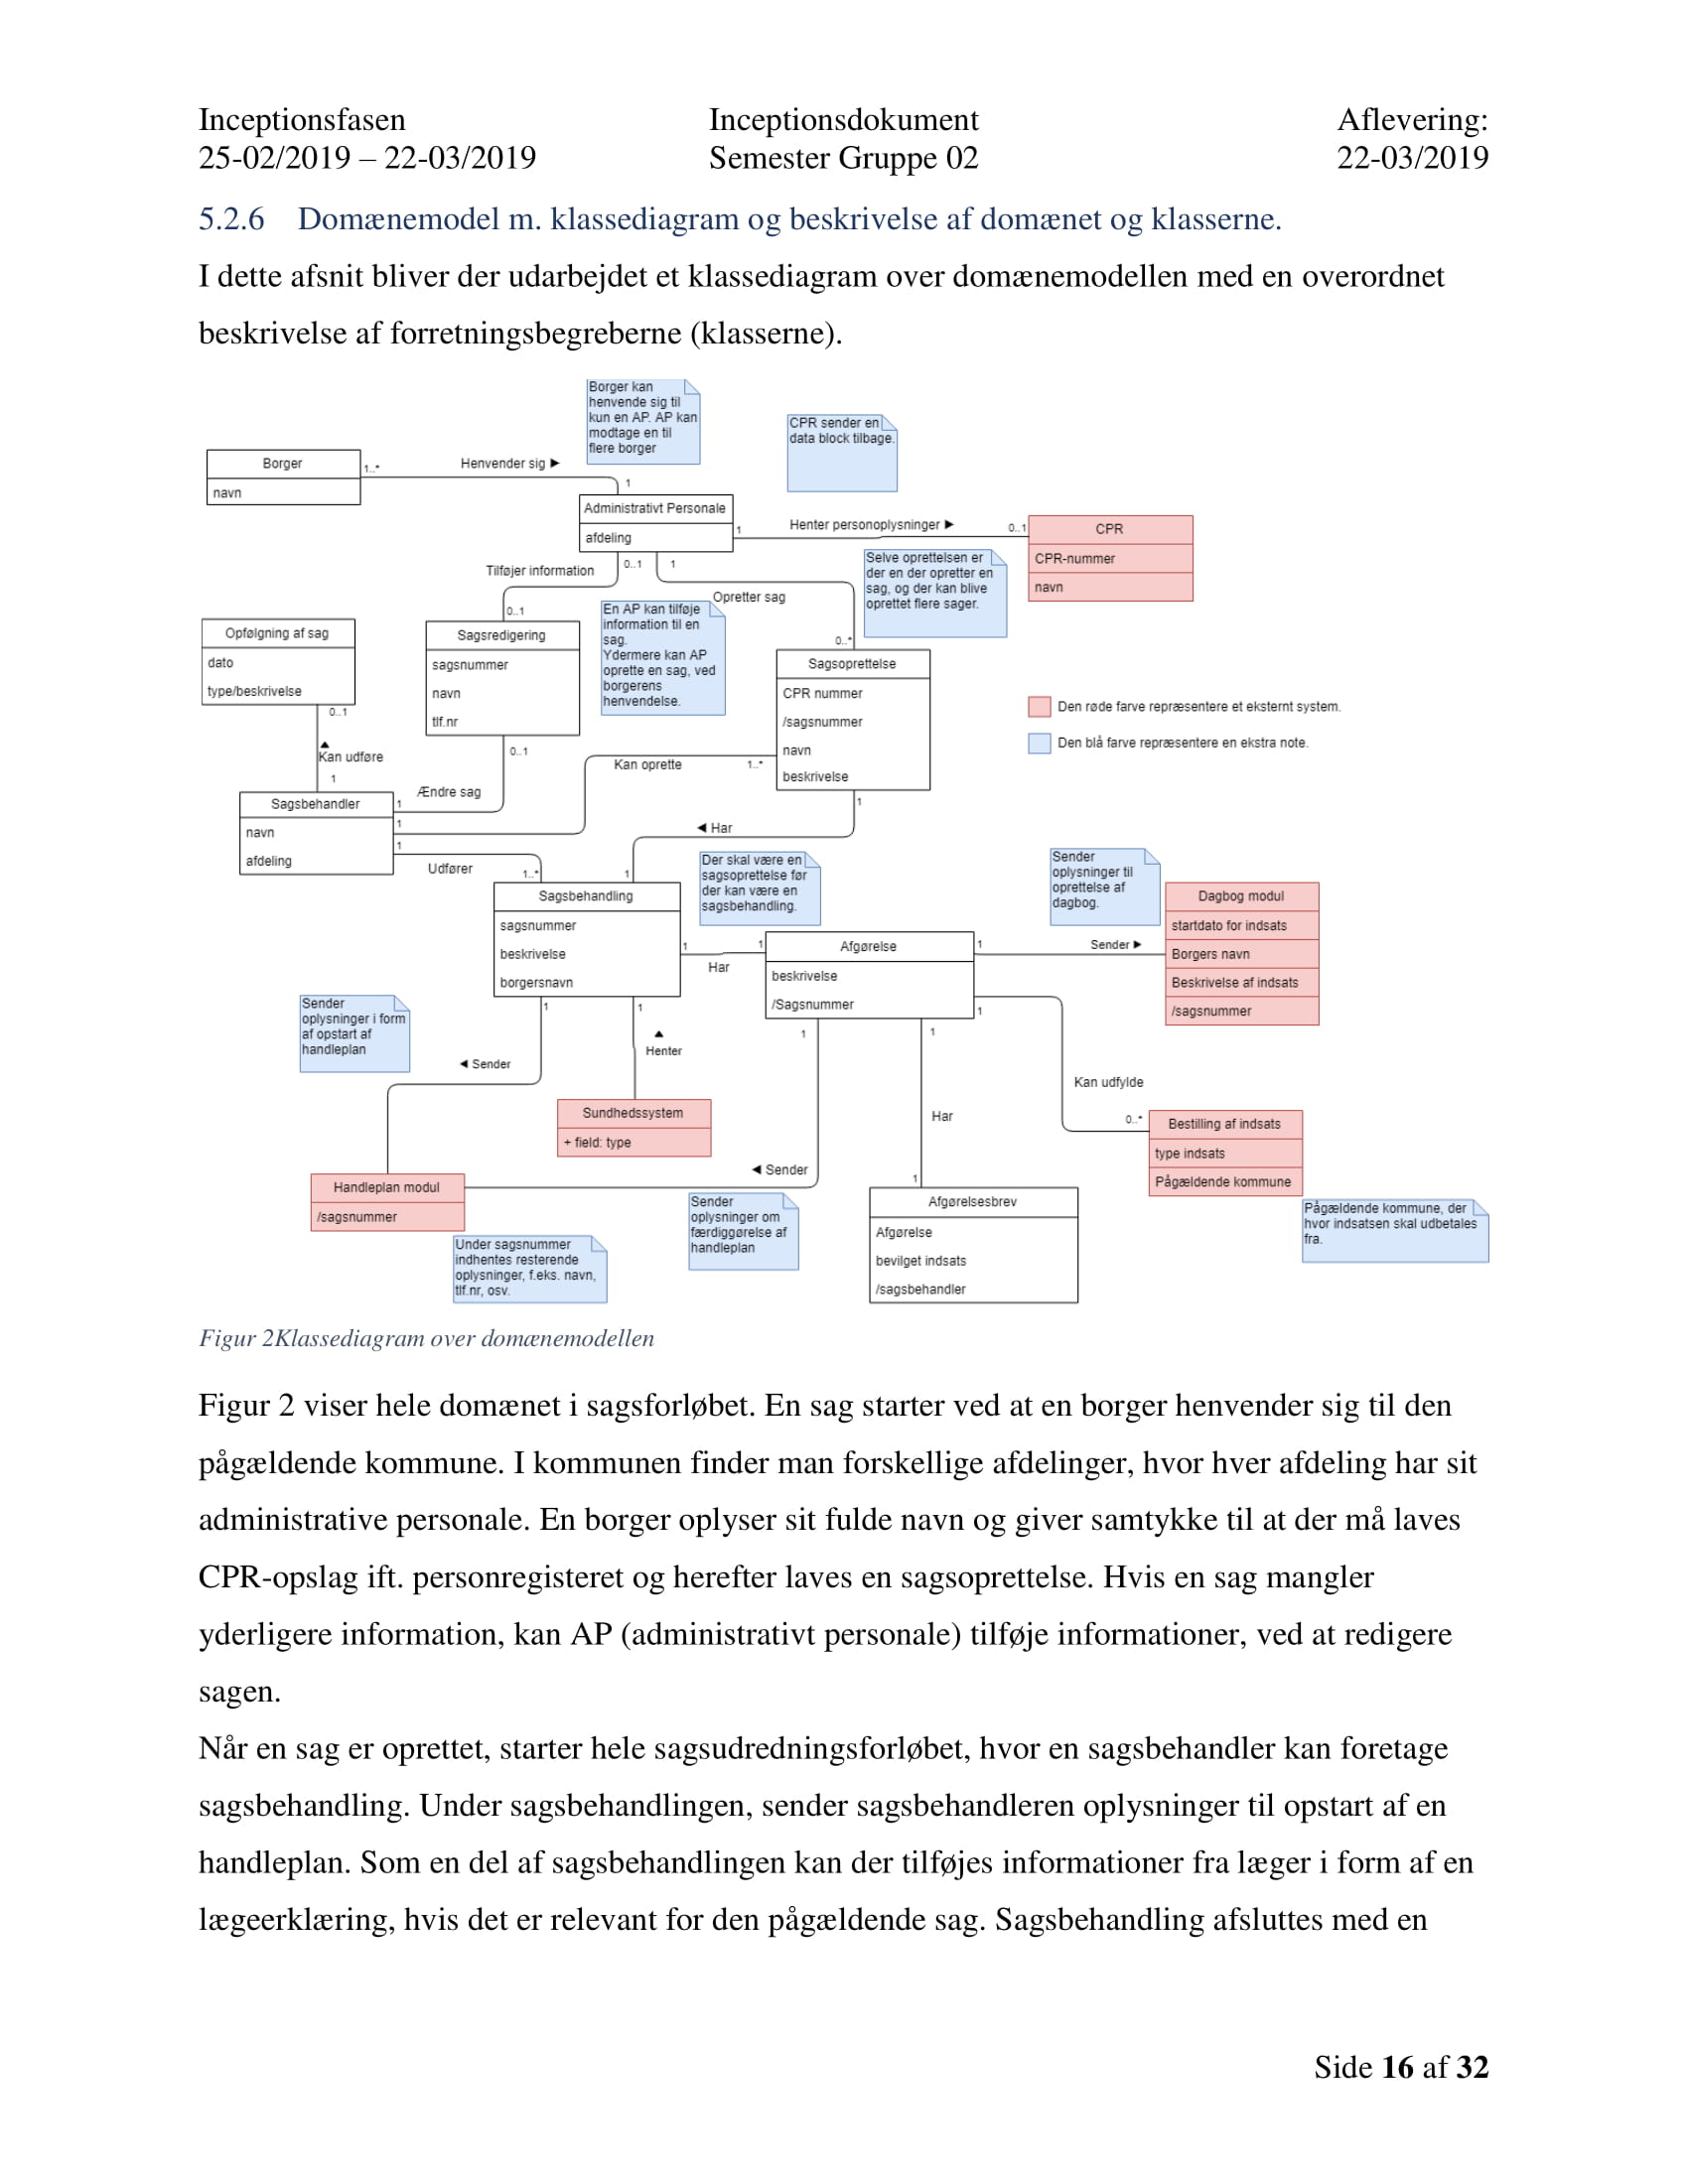
\includegraphics[scale = 0.33]{./PNG/Inceptions/Gruppe 02 + InceptionsDokument-17.jpg} 
\end{figure}

\begin{figure}[hb]
  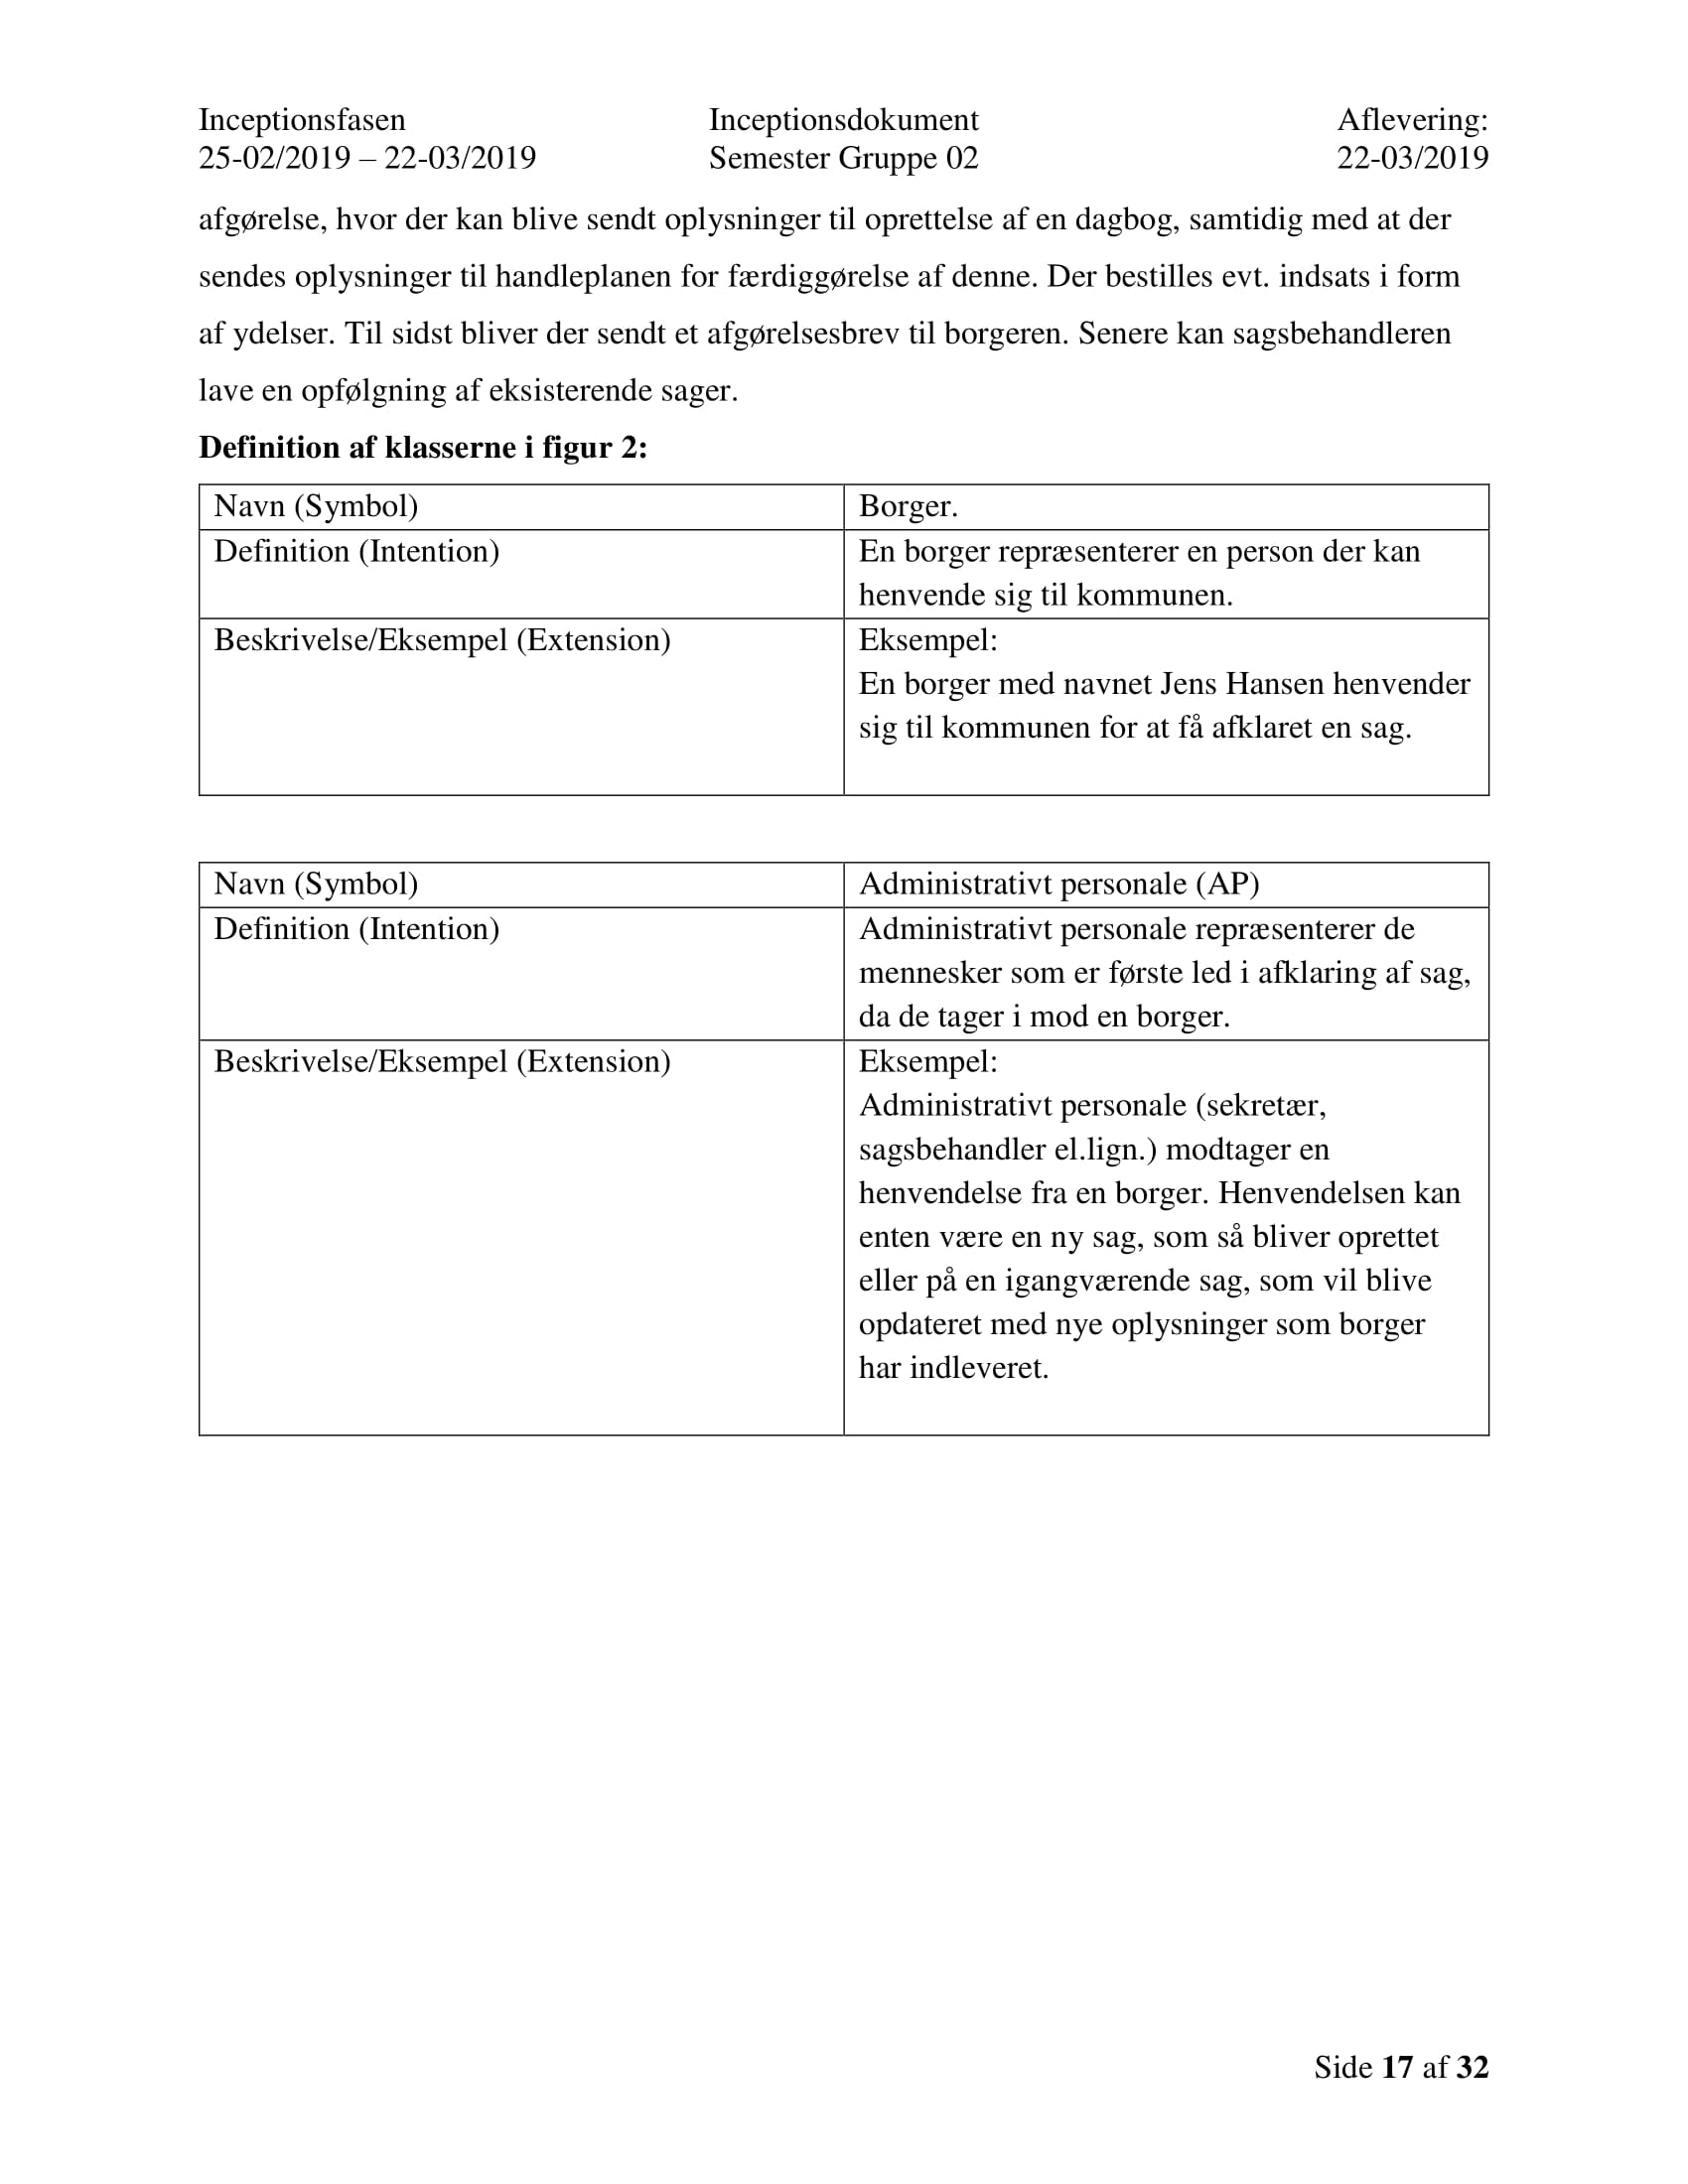
\includegraphics[scale = 0.33]{./PNG/Inceptions/Gruppe 02 + InceptionsDokument-18.jpg} 
\end{figure}

\begin{figure}[hb]
  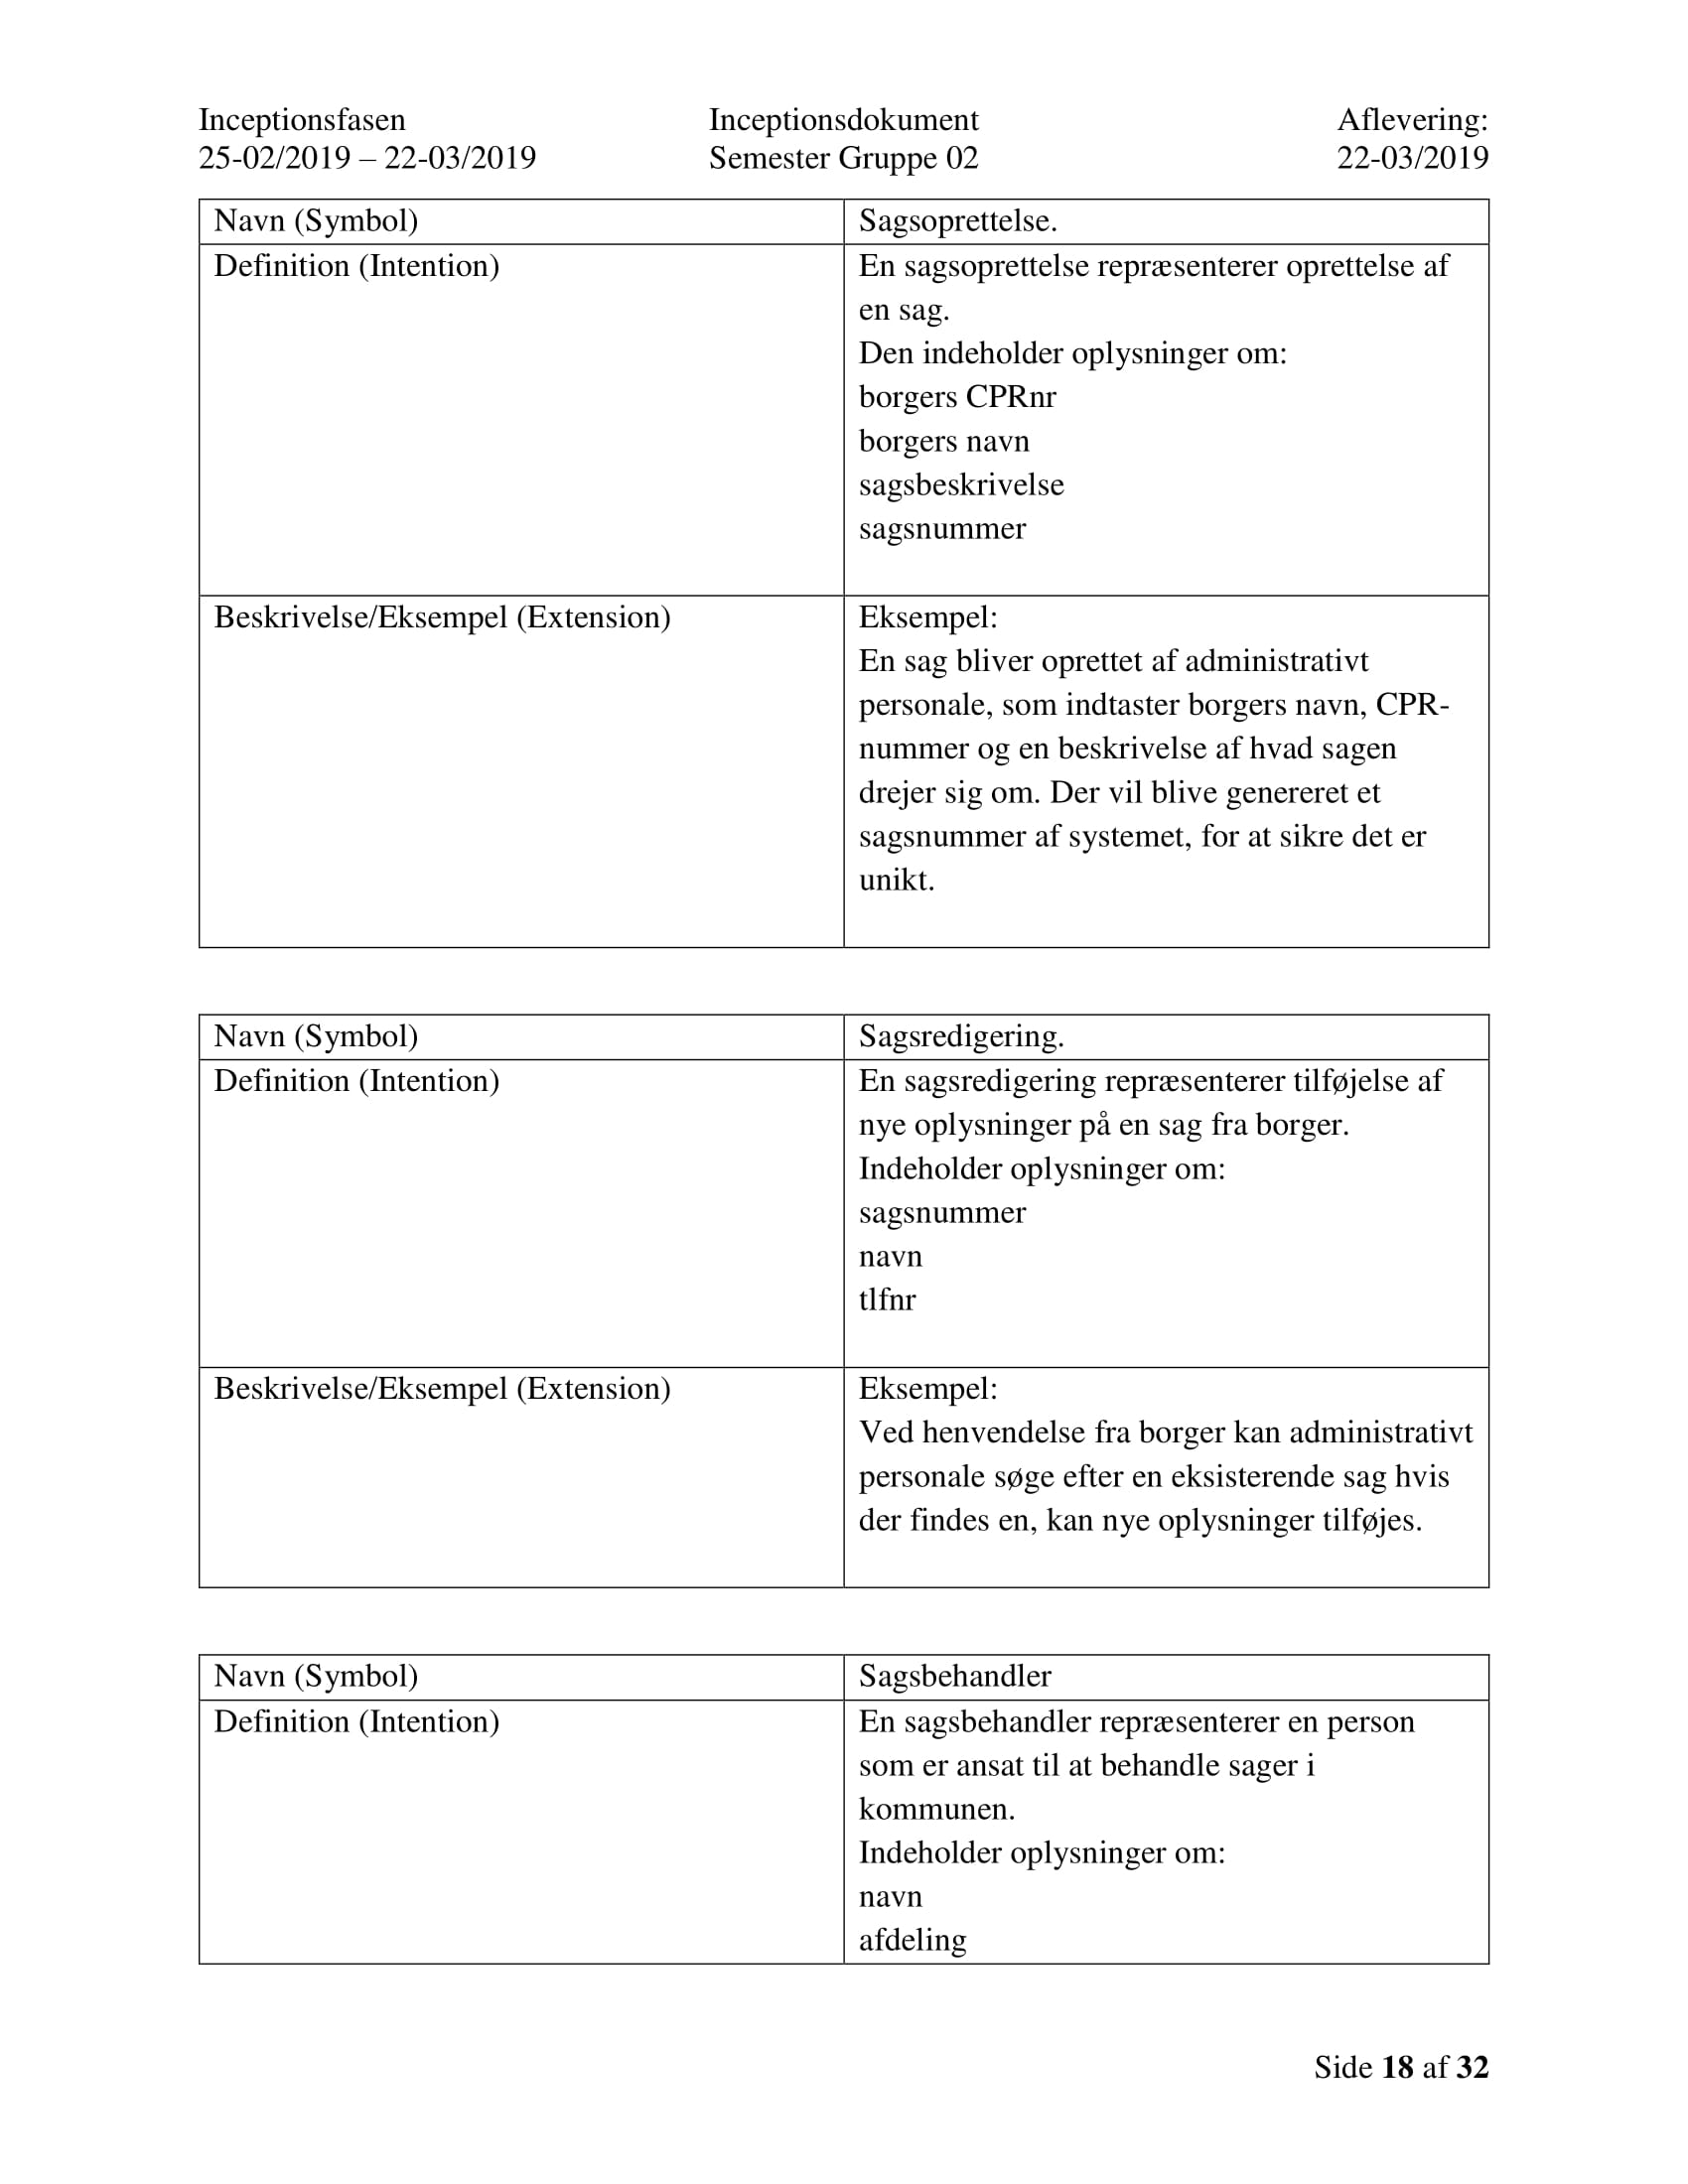
\includegraphics[scale = 0.33]{./PNG/Inceptions/Gruppe 02 + InceptionsDokument-19.jpg} 
\end{figure}

\begin{figure}[hb]
  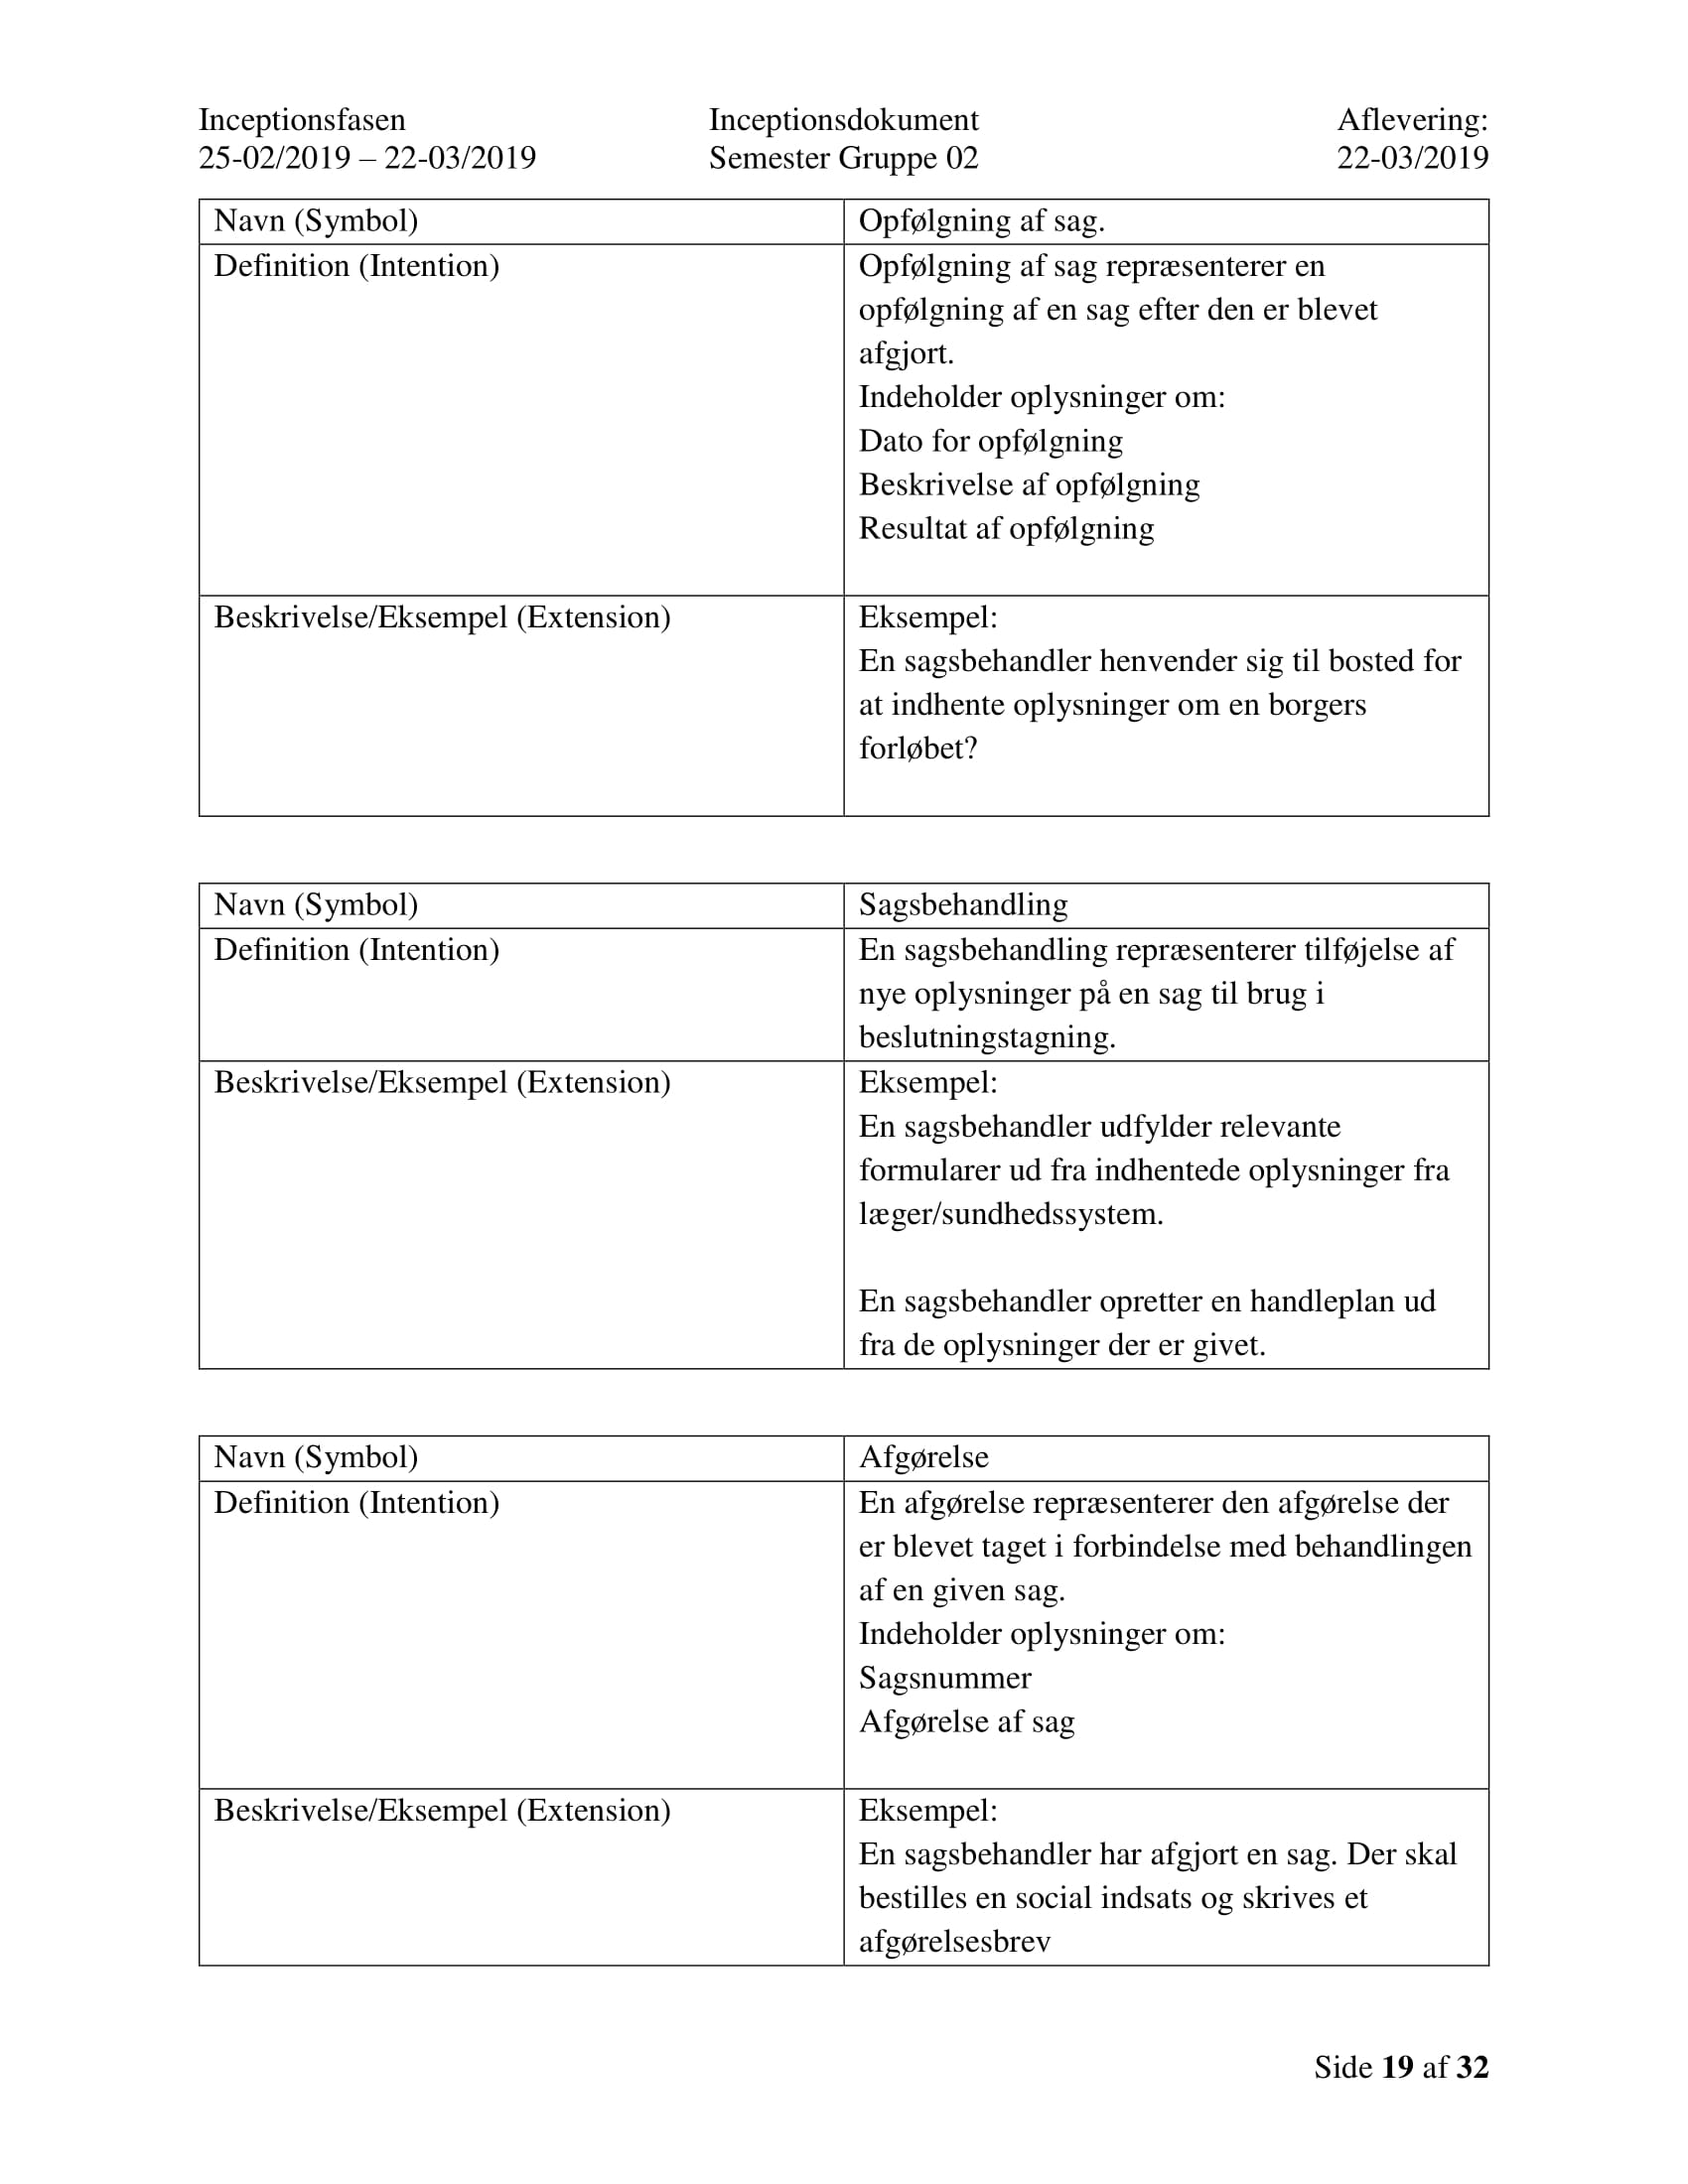
\includegraphics[scale = 0.33]{./PNG/Inceptions/Gruppe 02 + InceptionsDokument-20.jpg} 
\end{figure}

\begin{figure}[hb]
  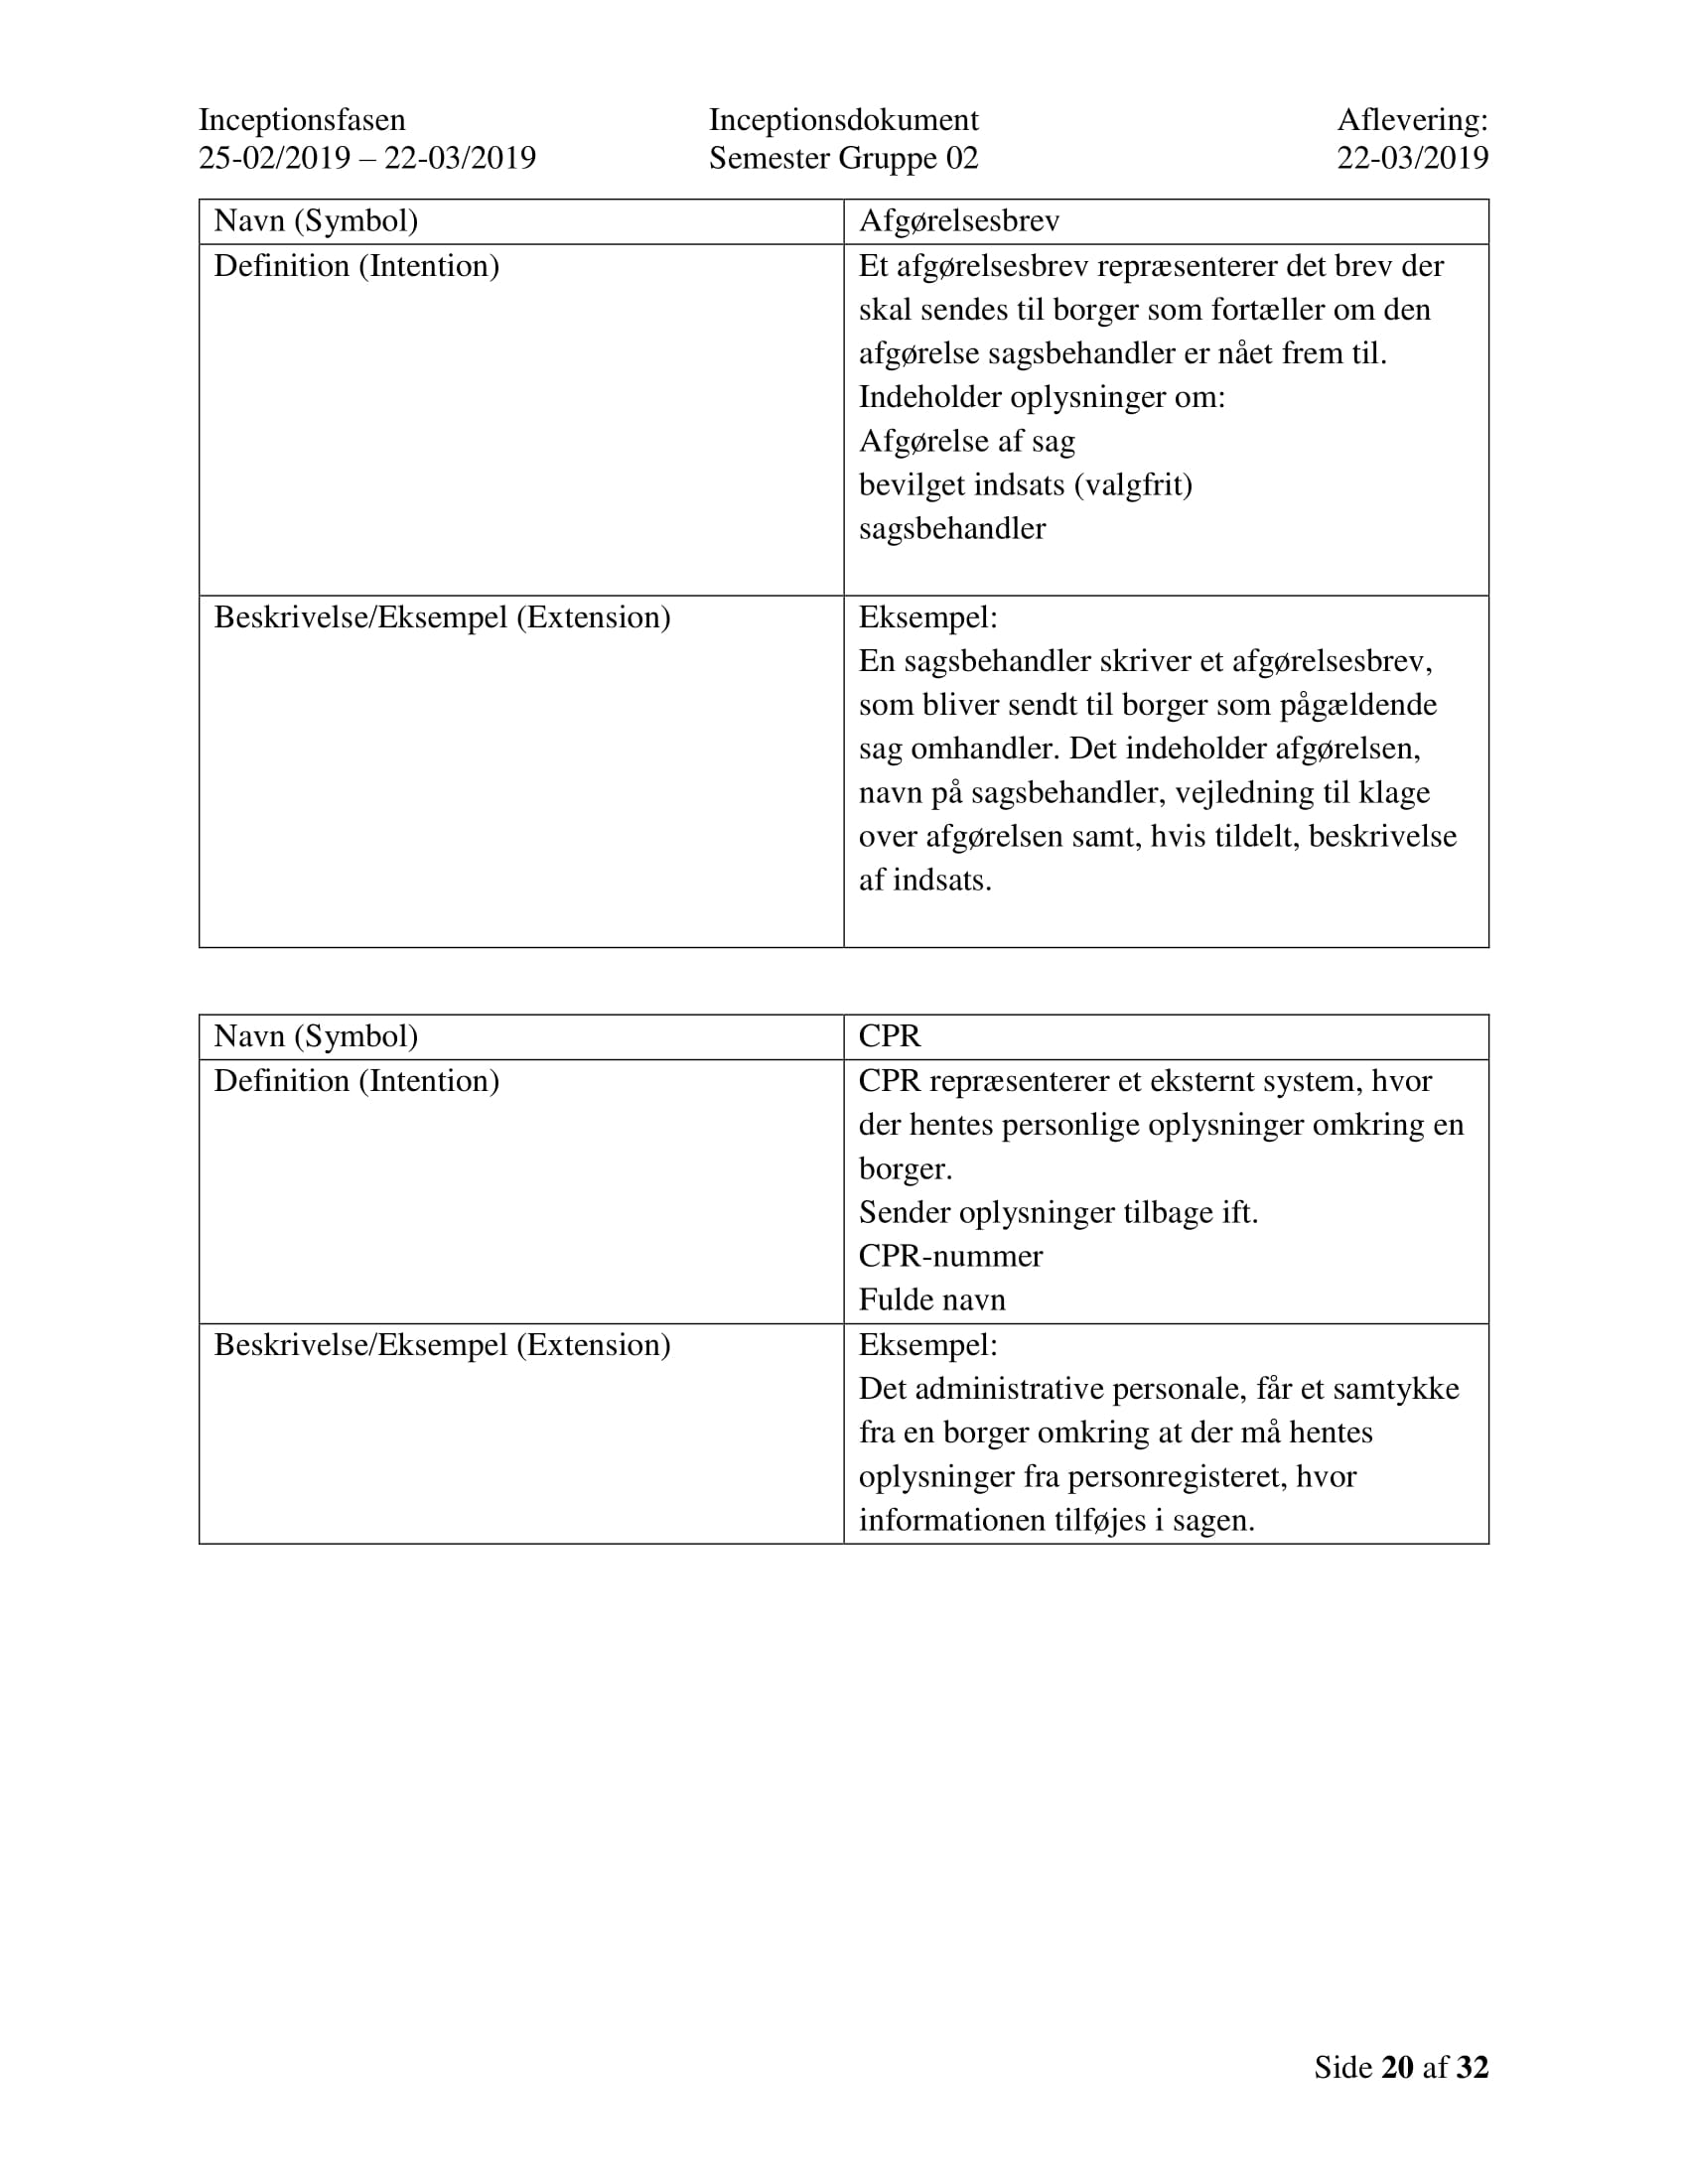
\includegraphics[scale = 0.33]{./PNG/Inceptions/Gruppe 02 + InceptionsDokument-21.jpg} 
\end{figure}

\begin{figure}[hb]
  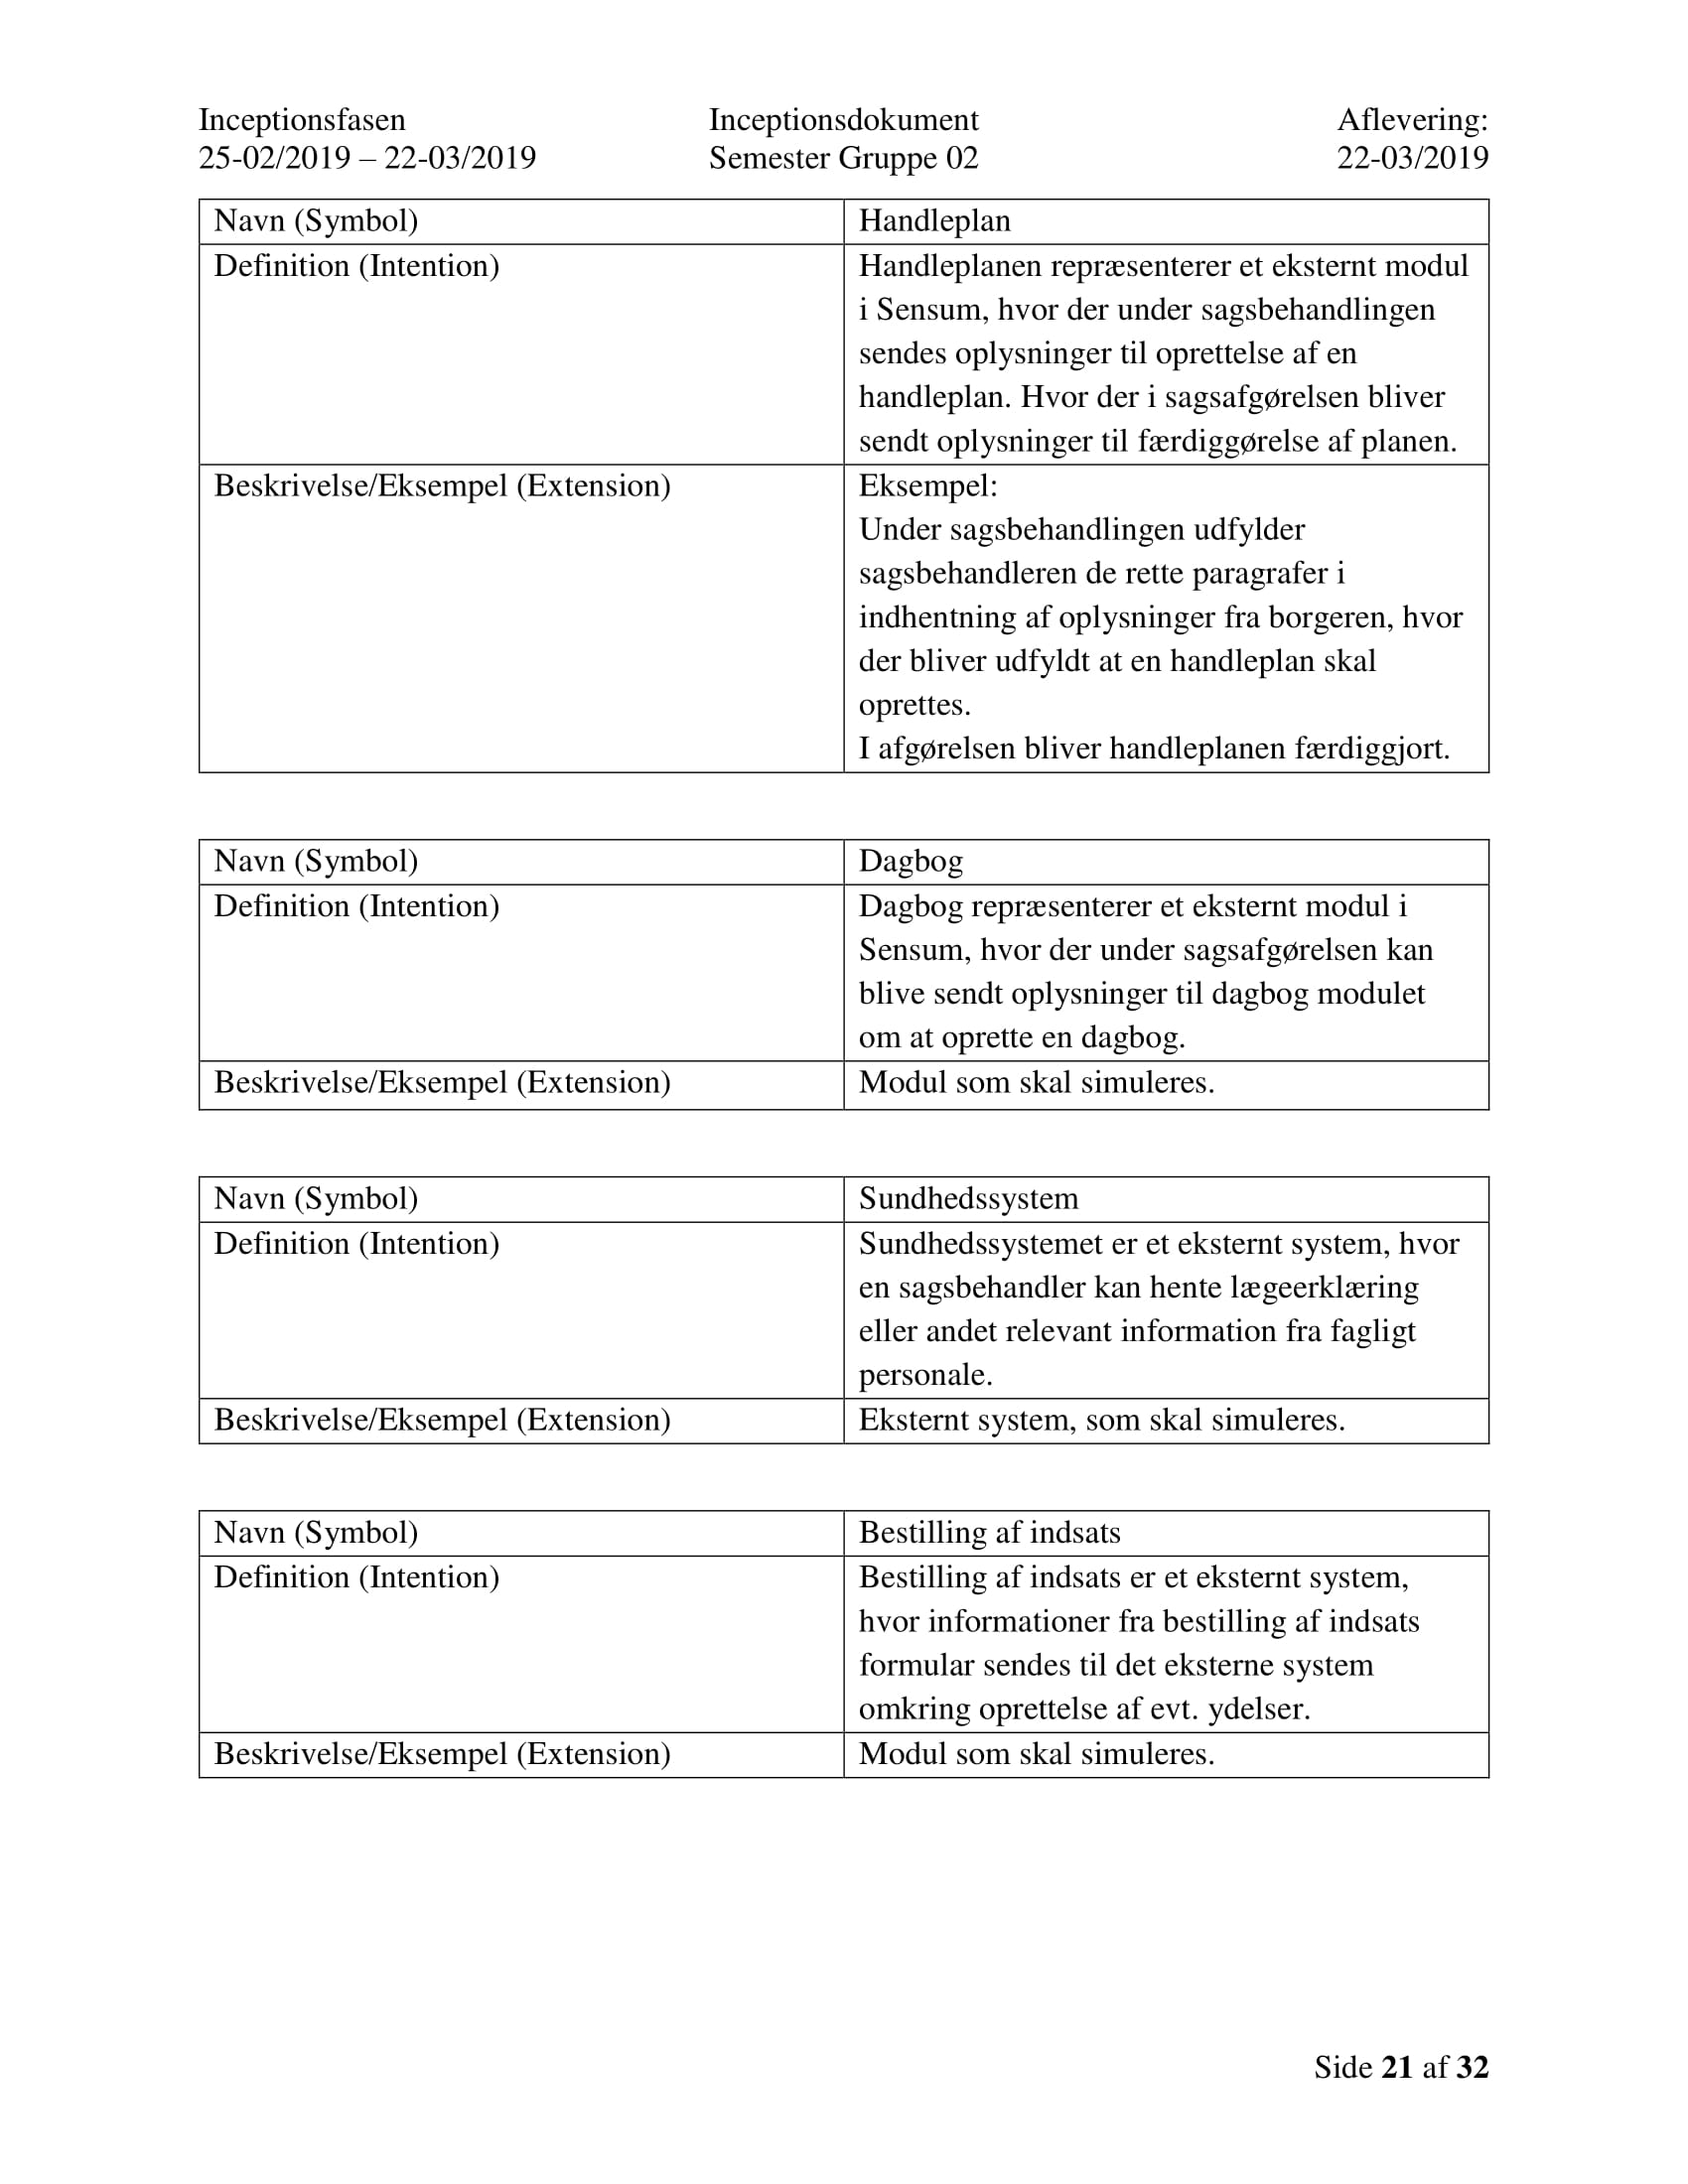
\includegraphics[scale = 0.33]{./PNG/Inceptions/Gruppe 02 + InceptionsDokument-22.jpg} 
\end{figure}

\begin{figure}[hb]
  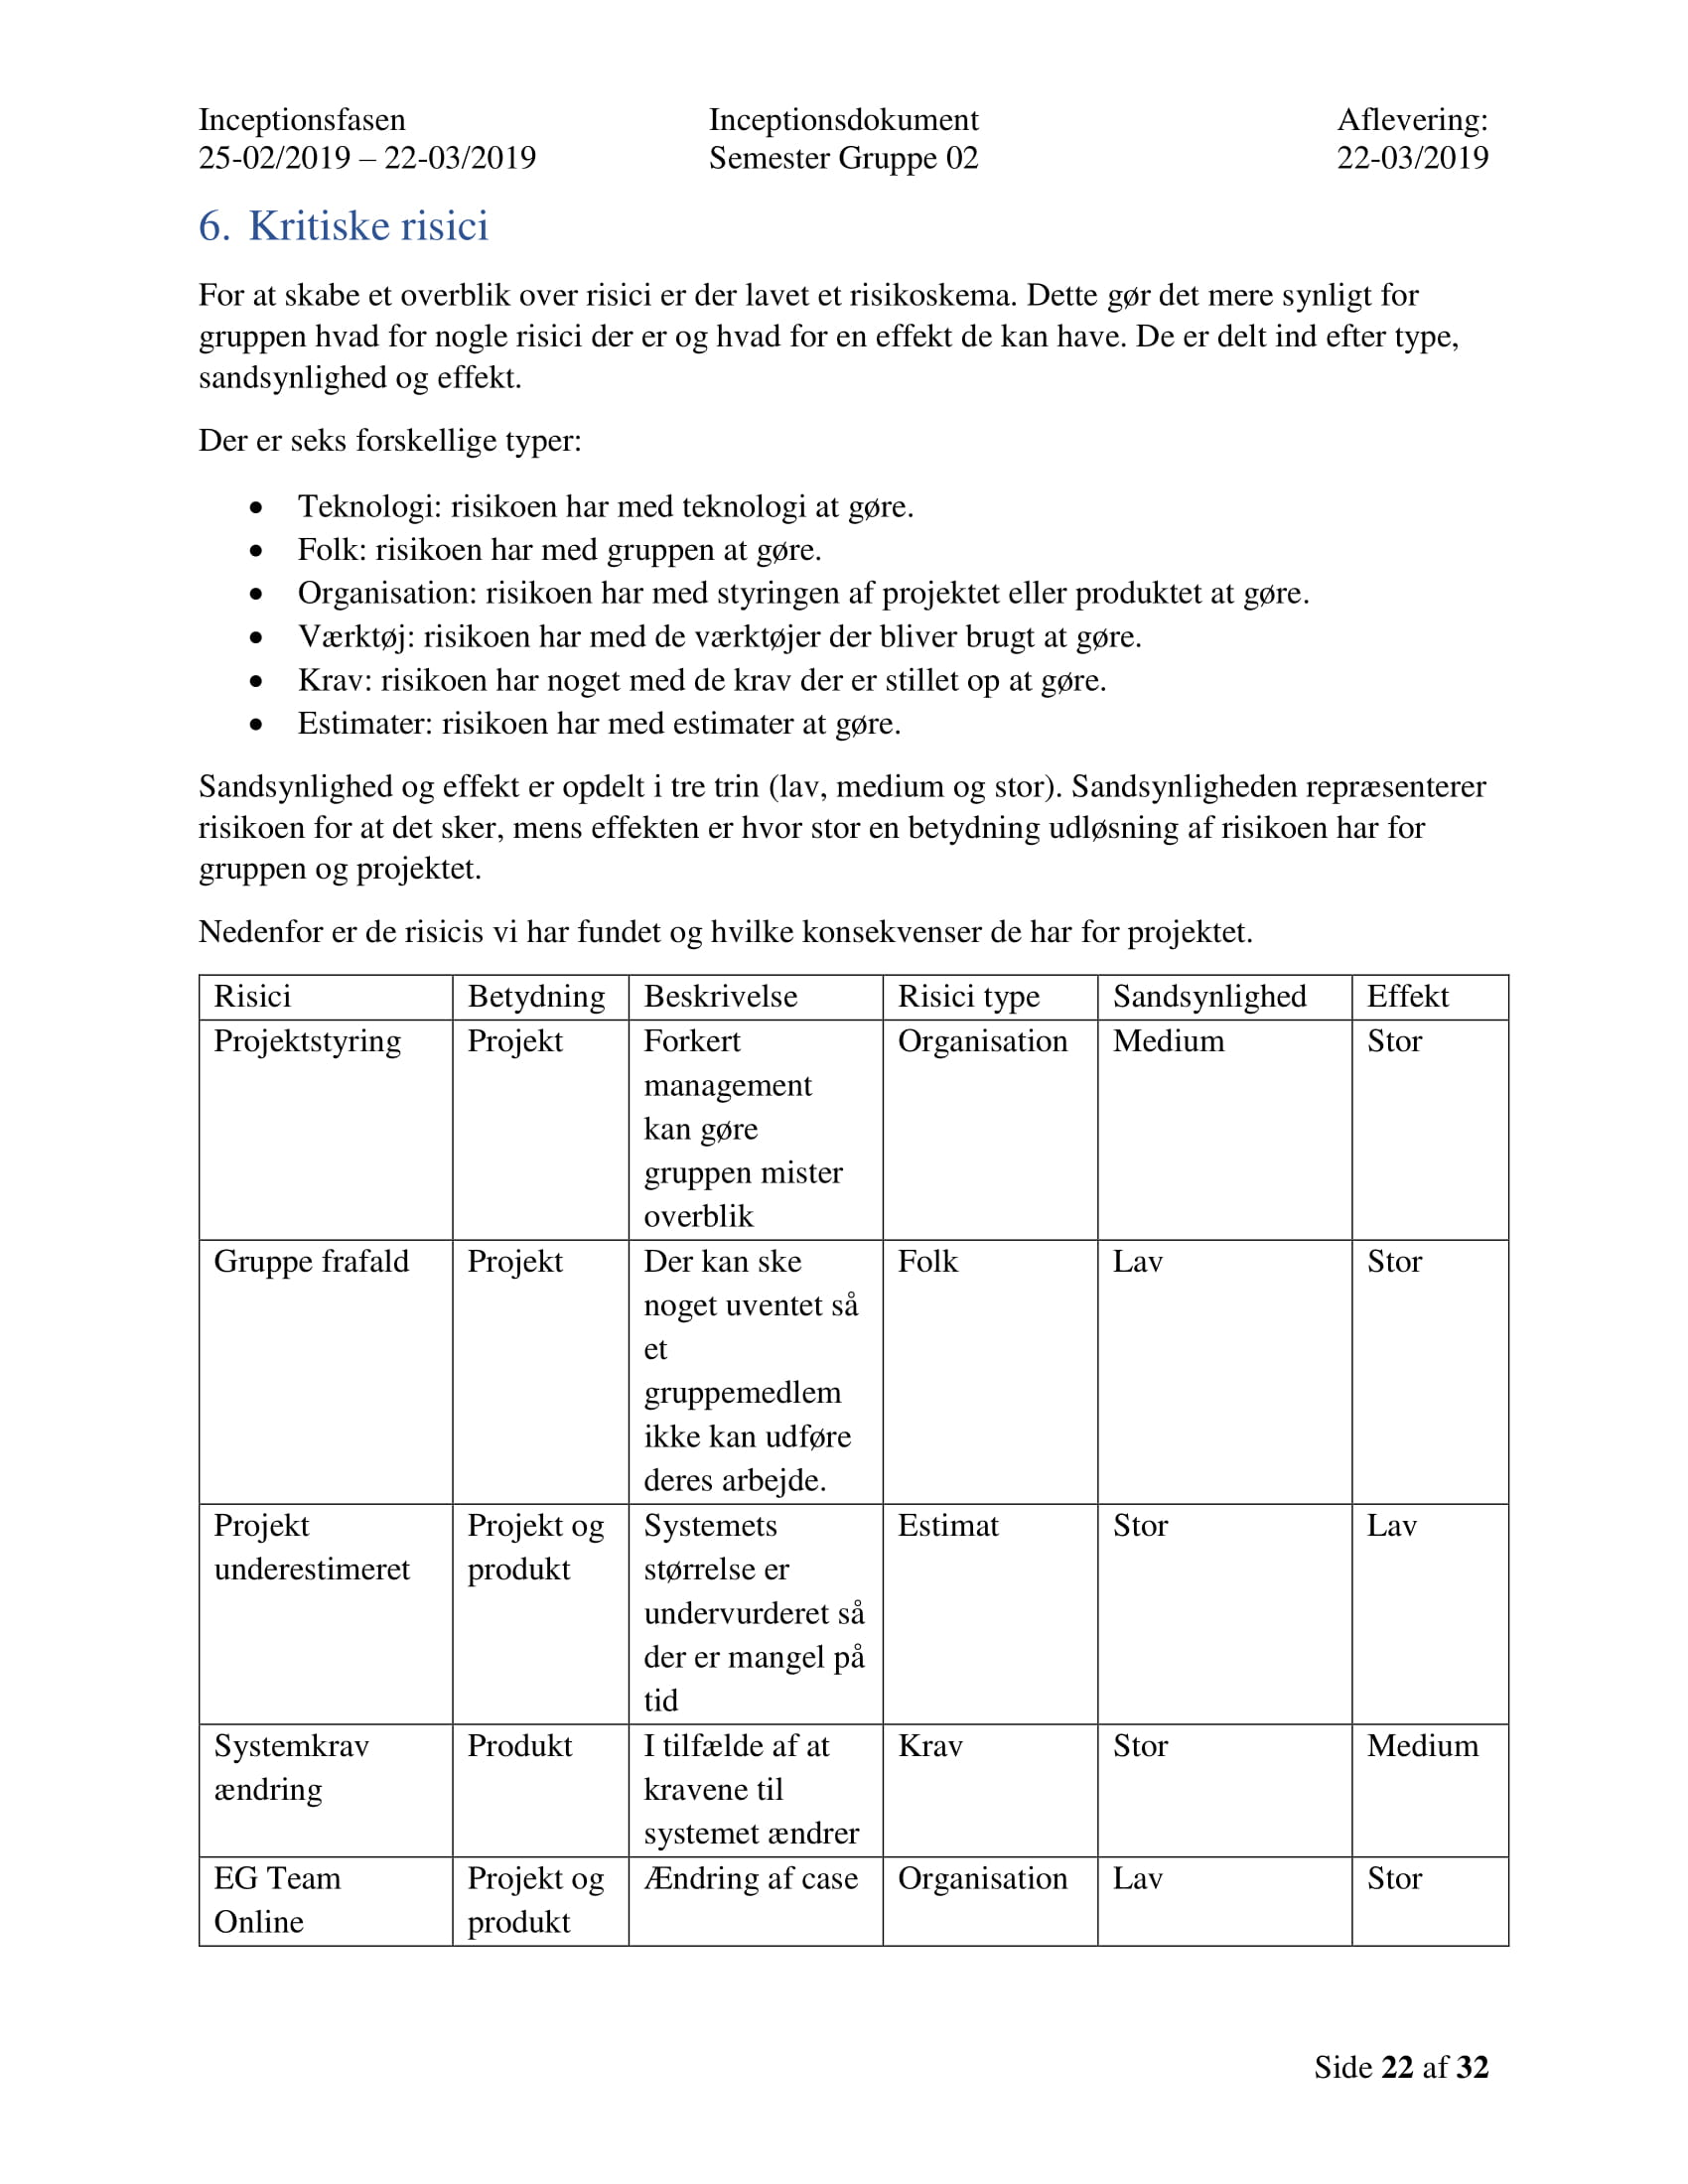
\includegraphics[scale = 0.33]{./PNG/Inceptions/Gruppe 02 + InceptionsDokument-23.jpg} 
\end{figure}

\begin{figure}[hb]
  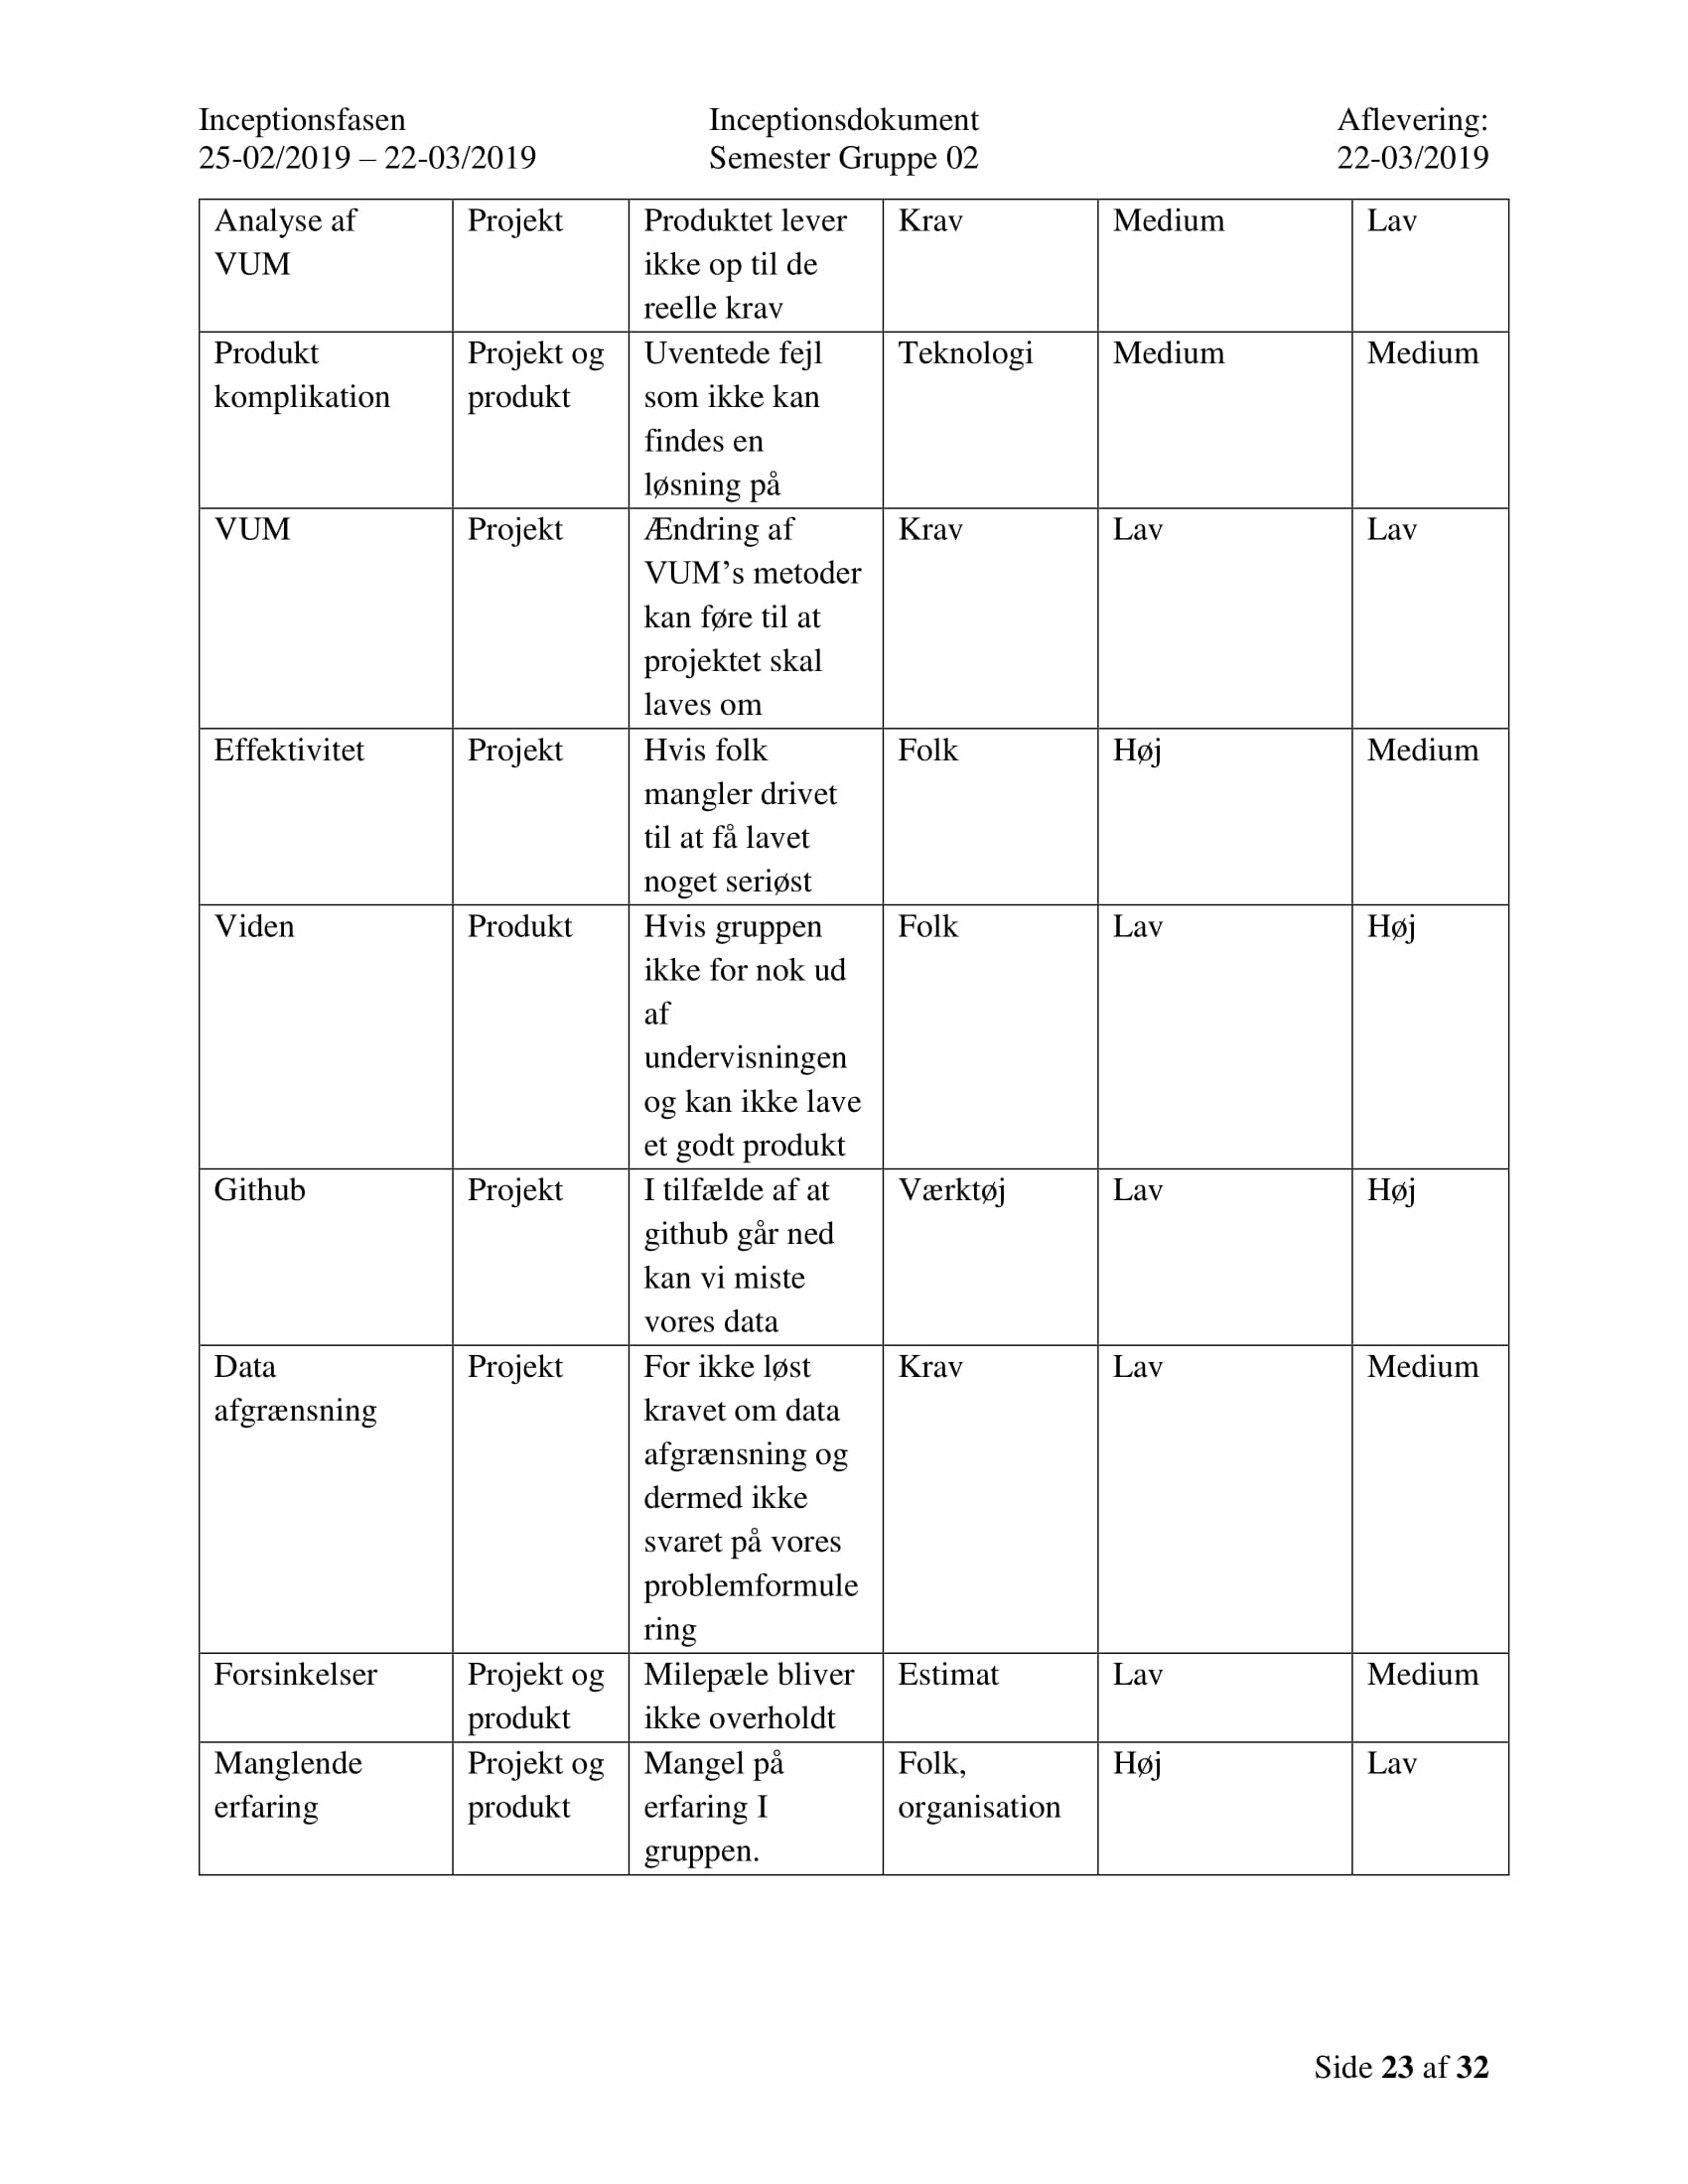
\includegraphics[scale = 0.33]{./PNG/Inceptions/Gruppe 02 + InceptionsDokument-24.jpg} 
\end{figure}

\begin{figure}[hb]
  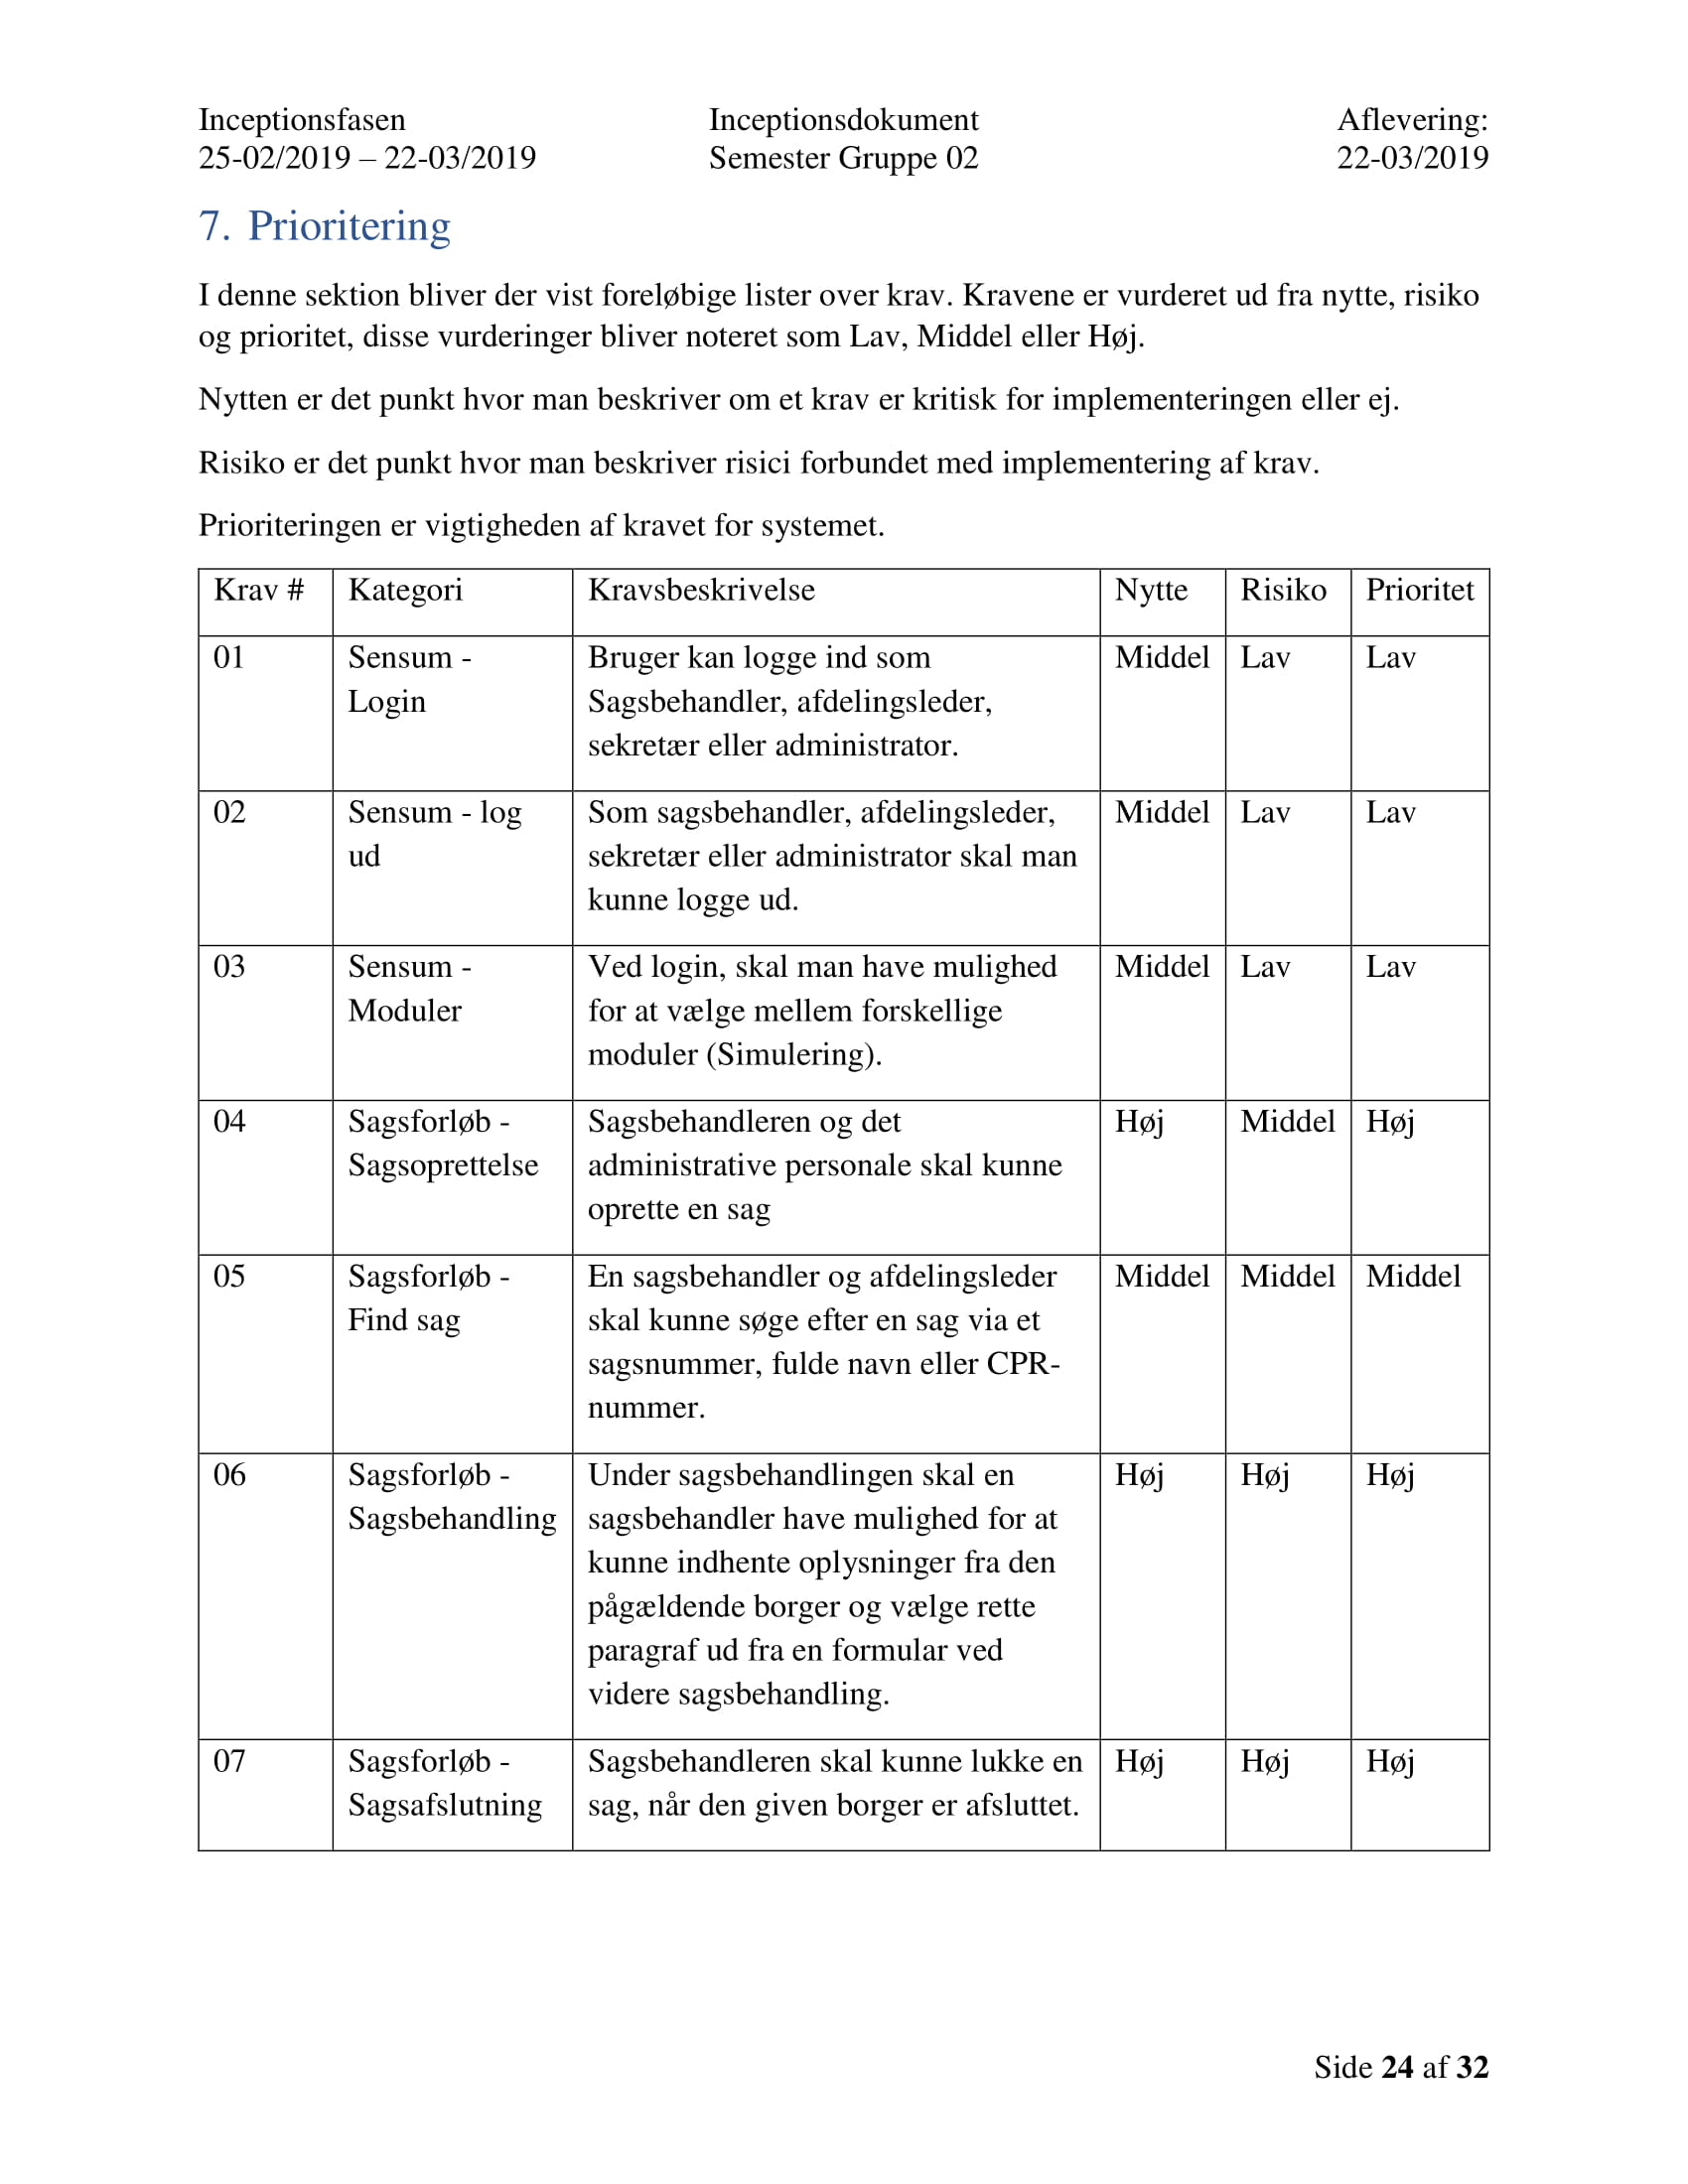
\includegraphics[scale = 0.33]{./PNG/Inceptions/Gruppe 02 + InceptionsDokument-25.jpg} 
\end{figure}

\begin{figure}[hb]
  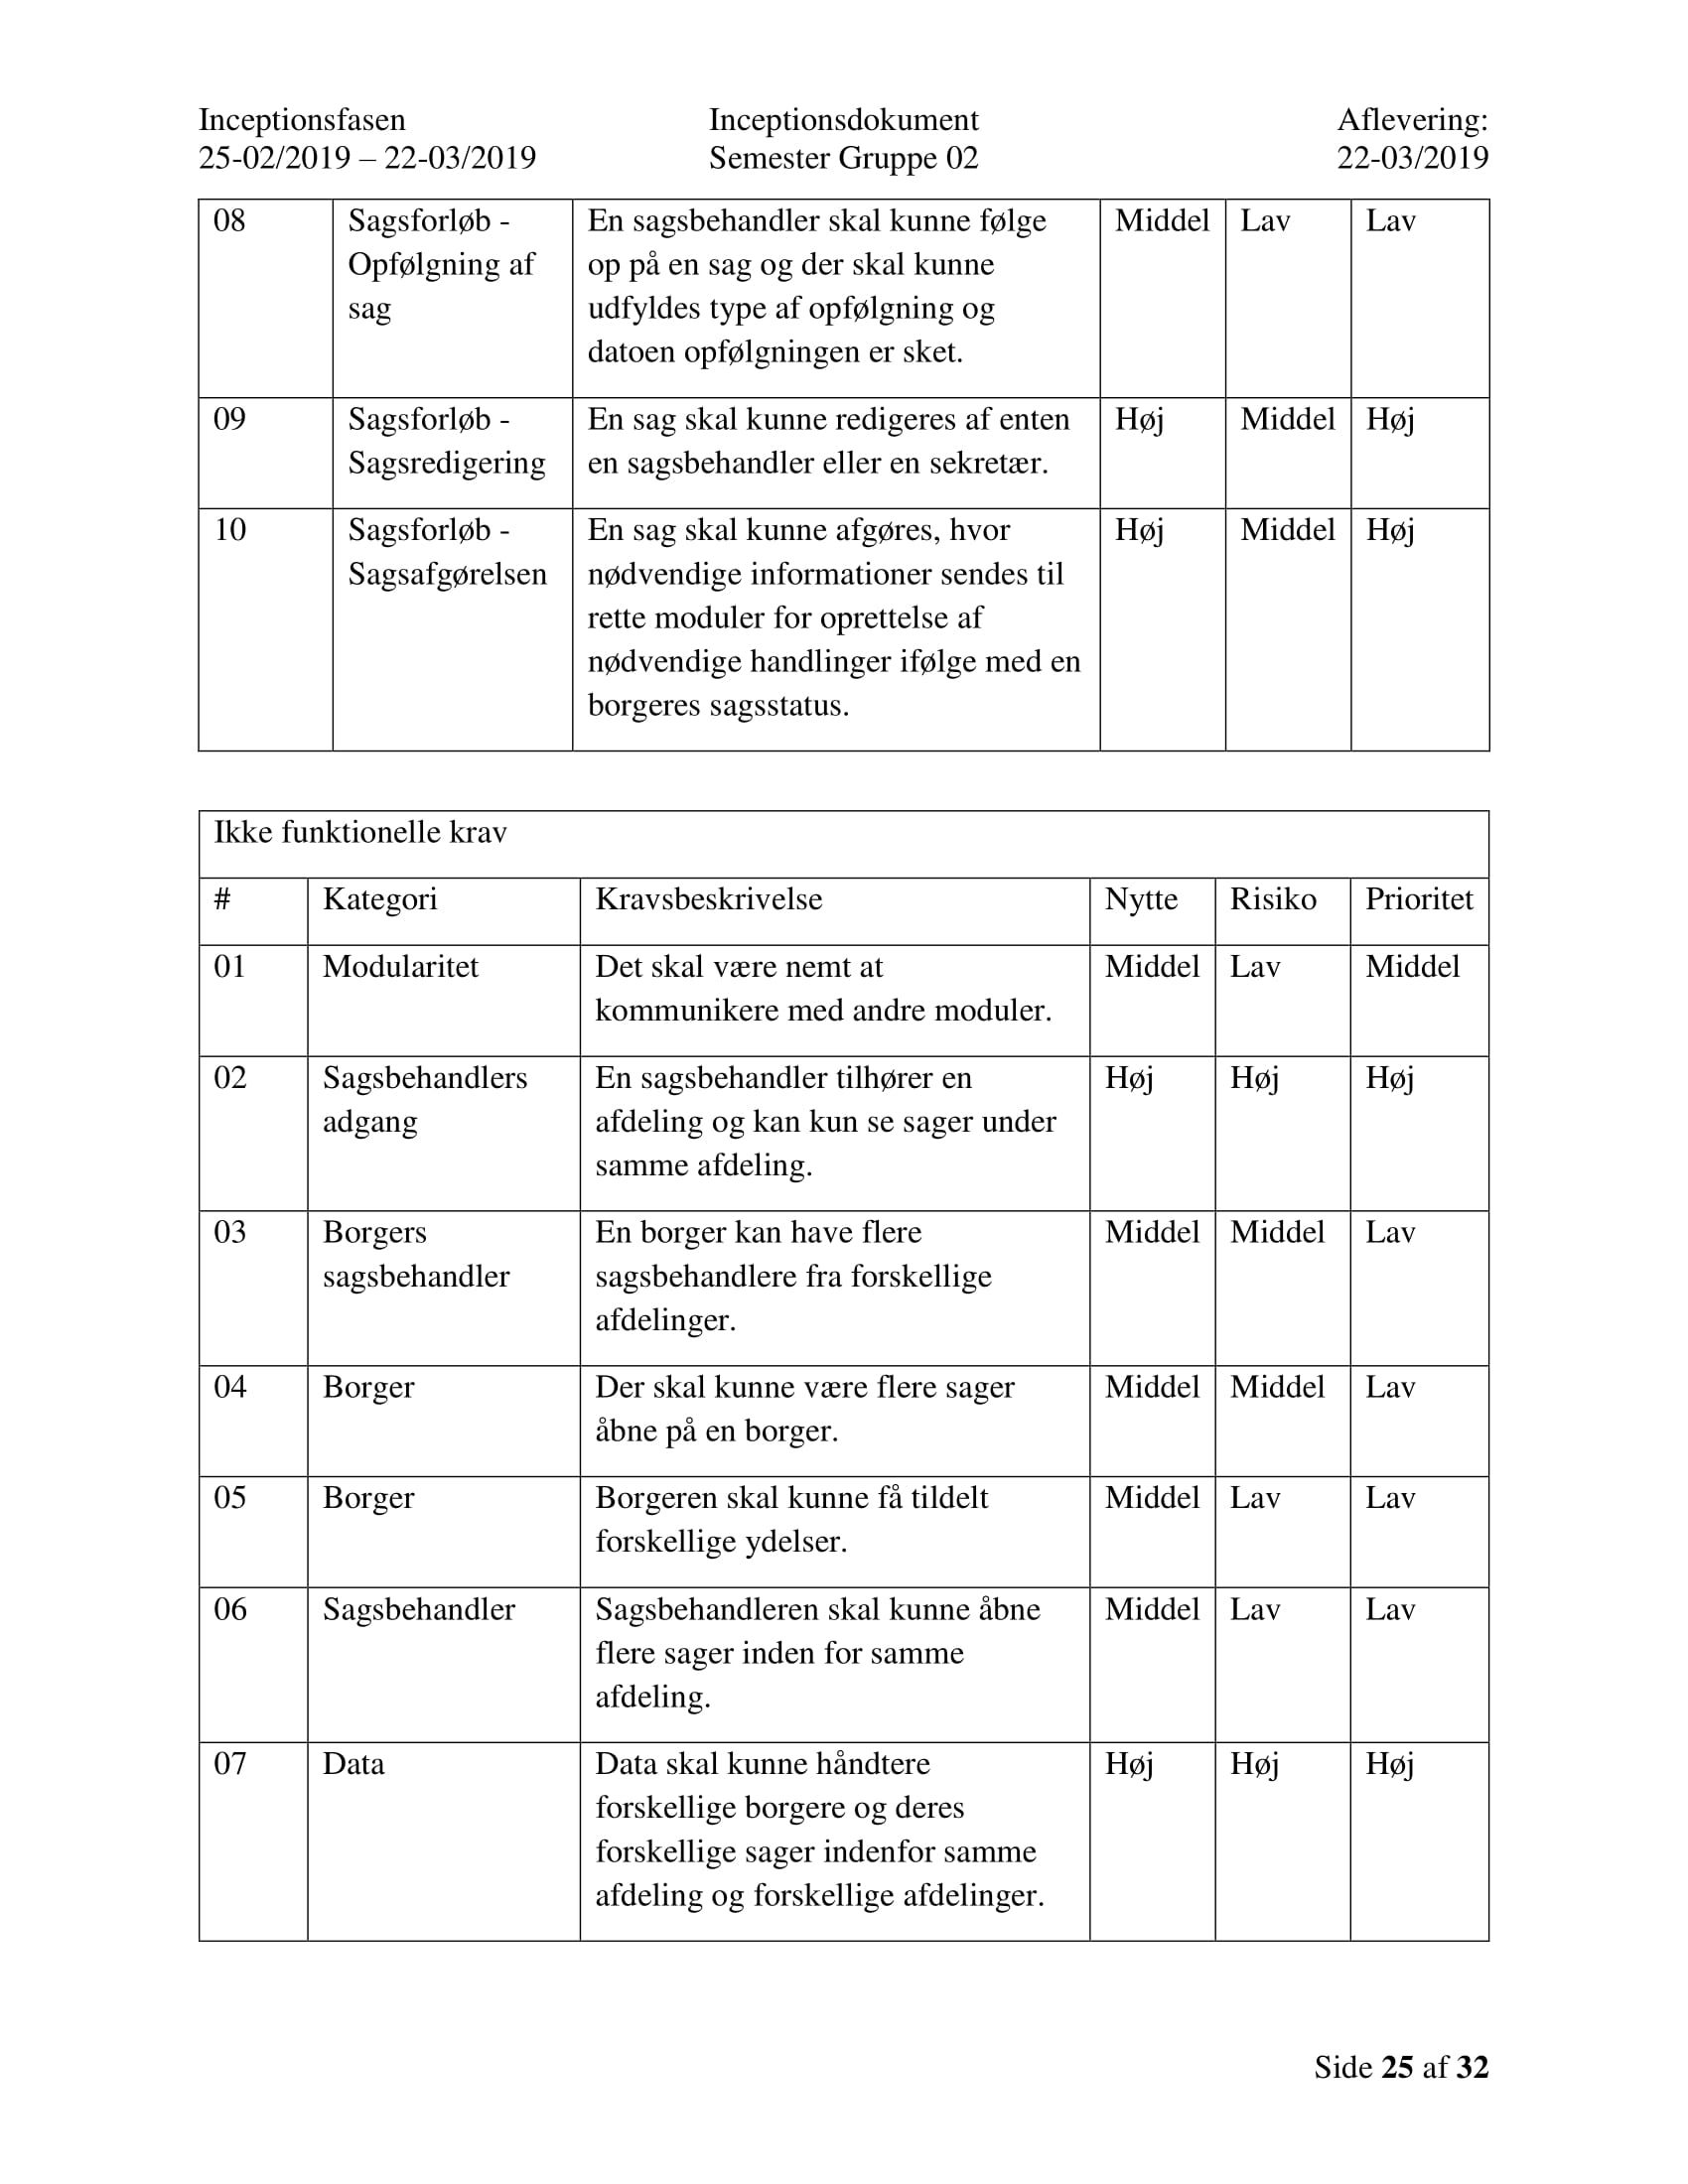
\includegraphics[scale = 0.33]{./PNG/Inceptions/Gruppe 02 + InceptionsDokument-26.jpg} 
\end{figure}

\begin{figure}[hb]
  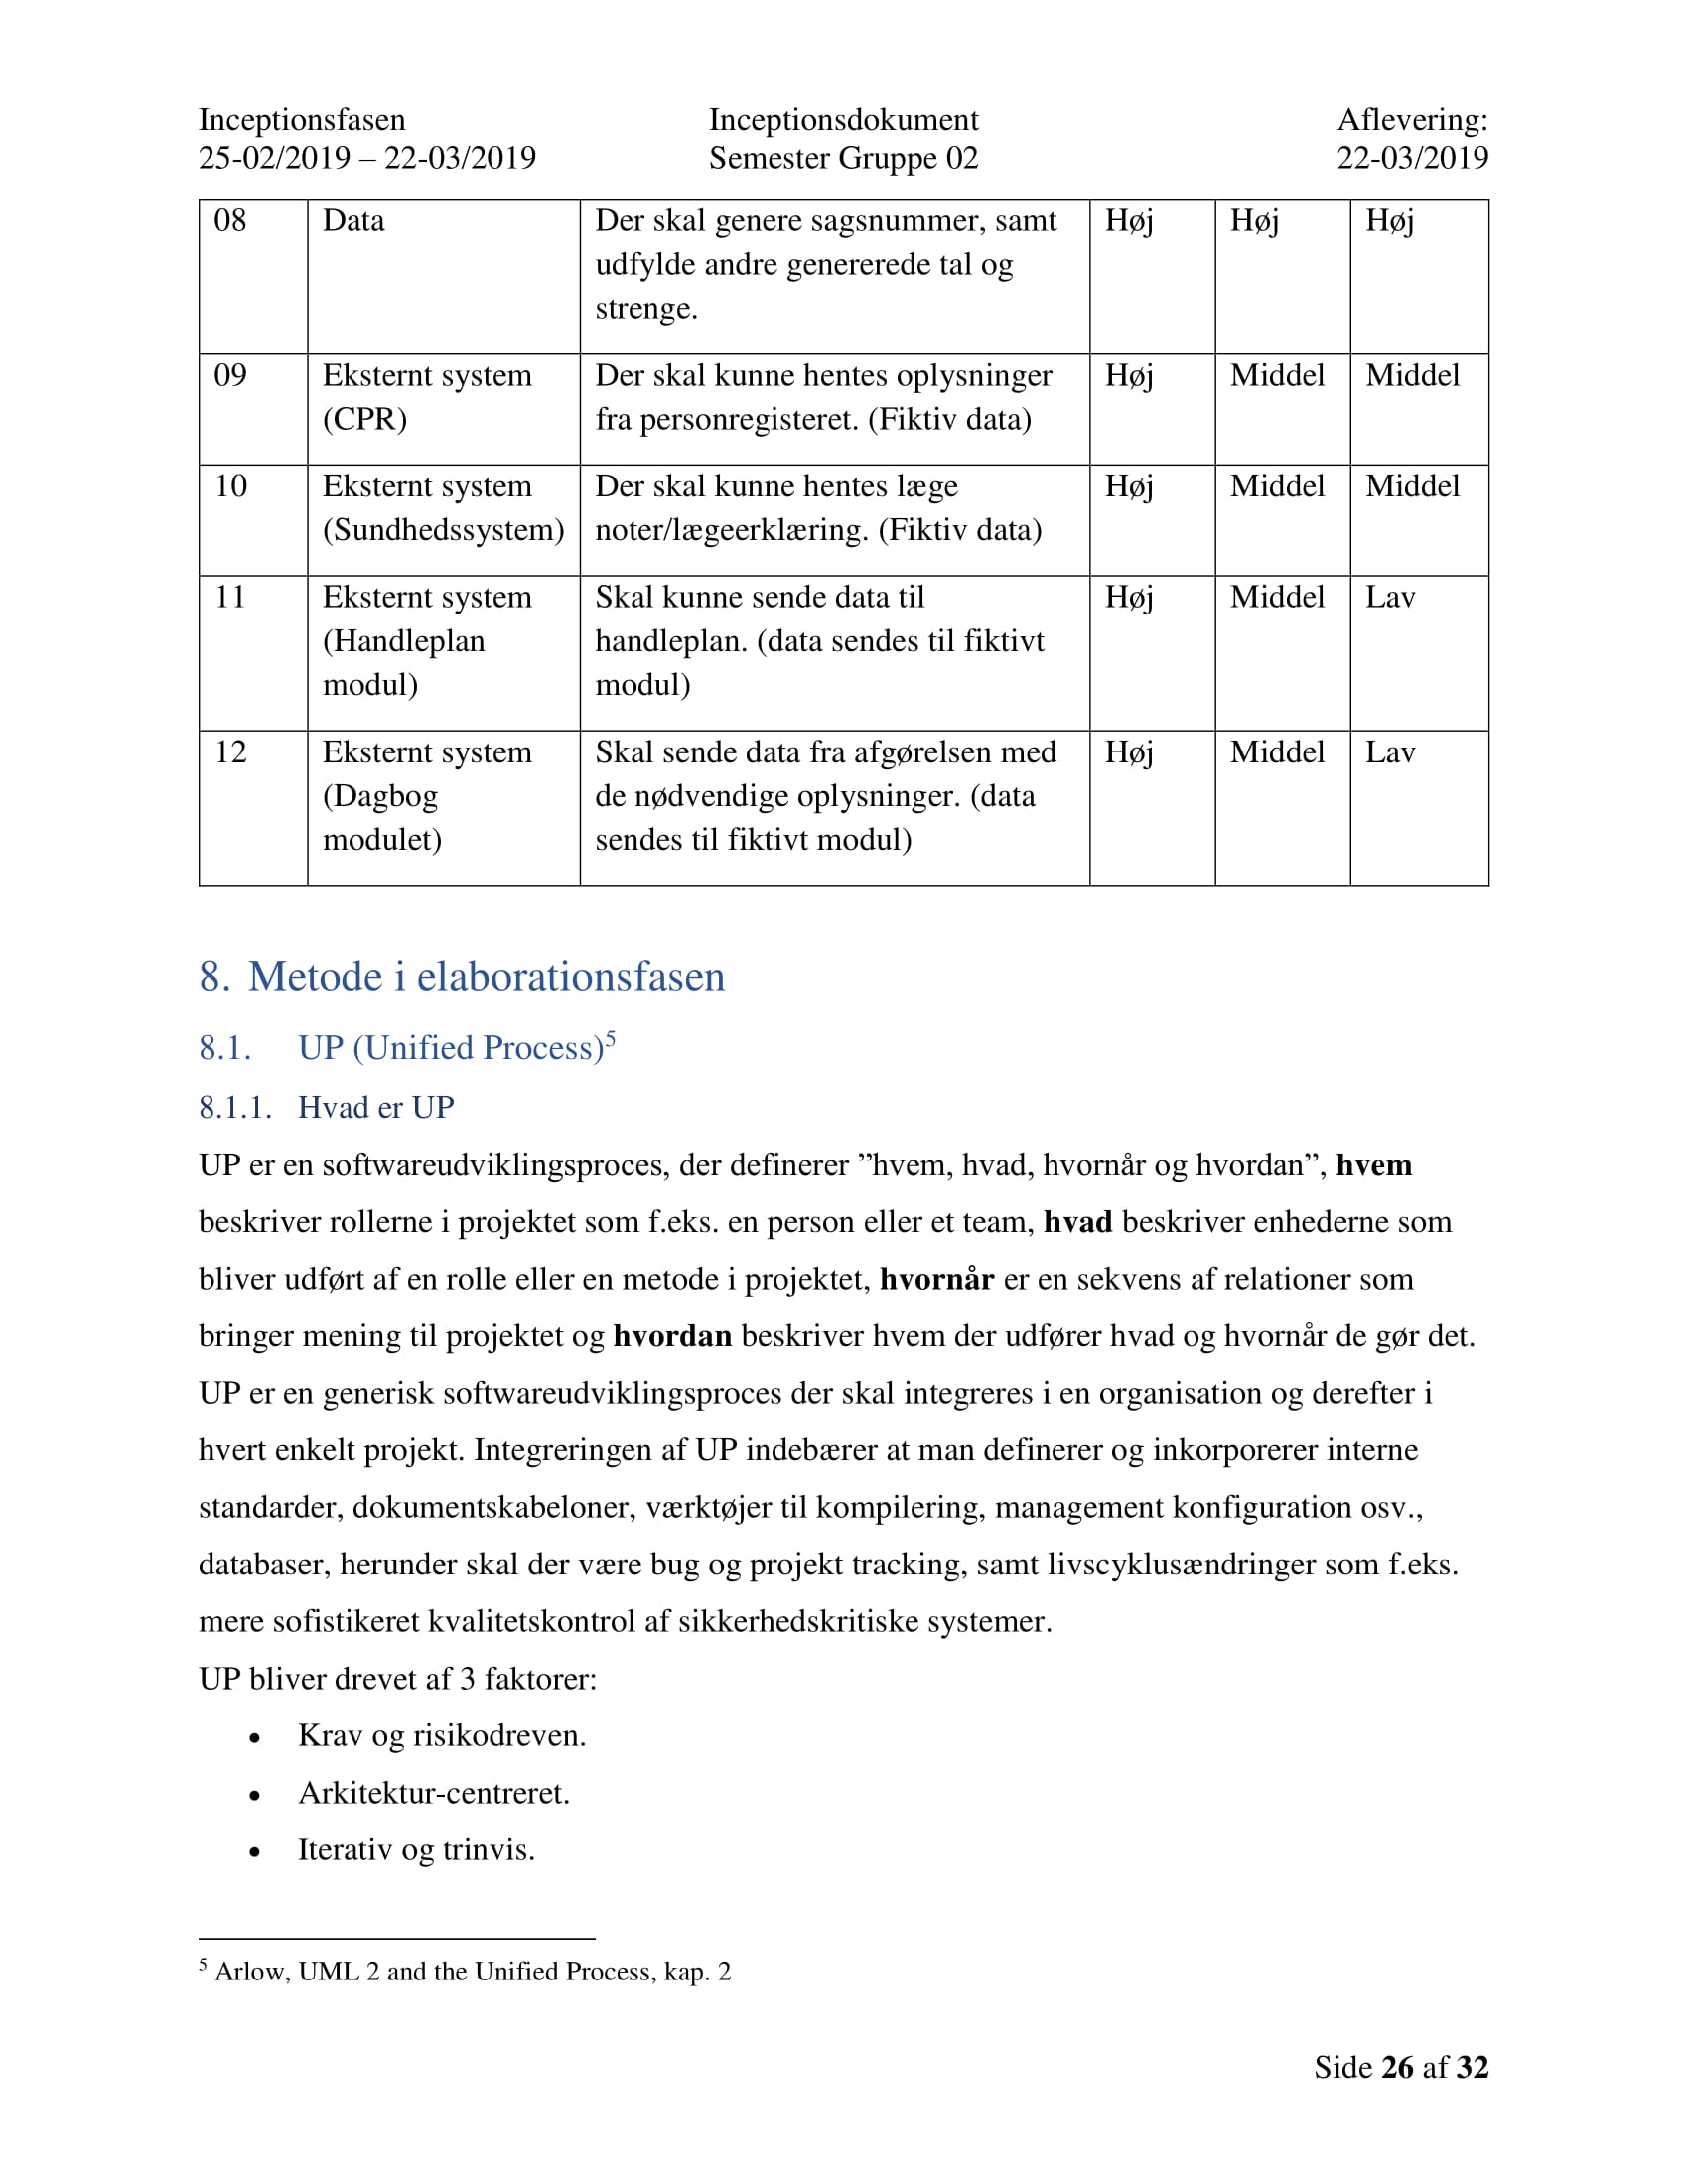
\includegraphics[scale = 0.33]{./PNG/Inceptions/Gruppe 02 + InceptionsDokument-27.jpg} 
\end{figure}

\begin{figure}[hb]
  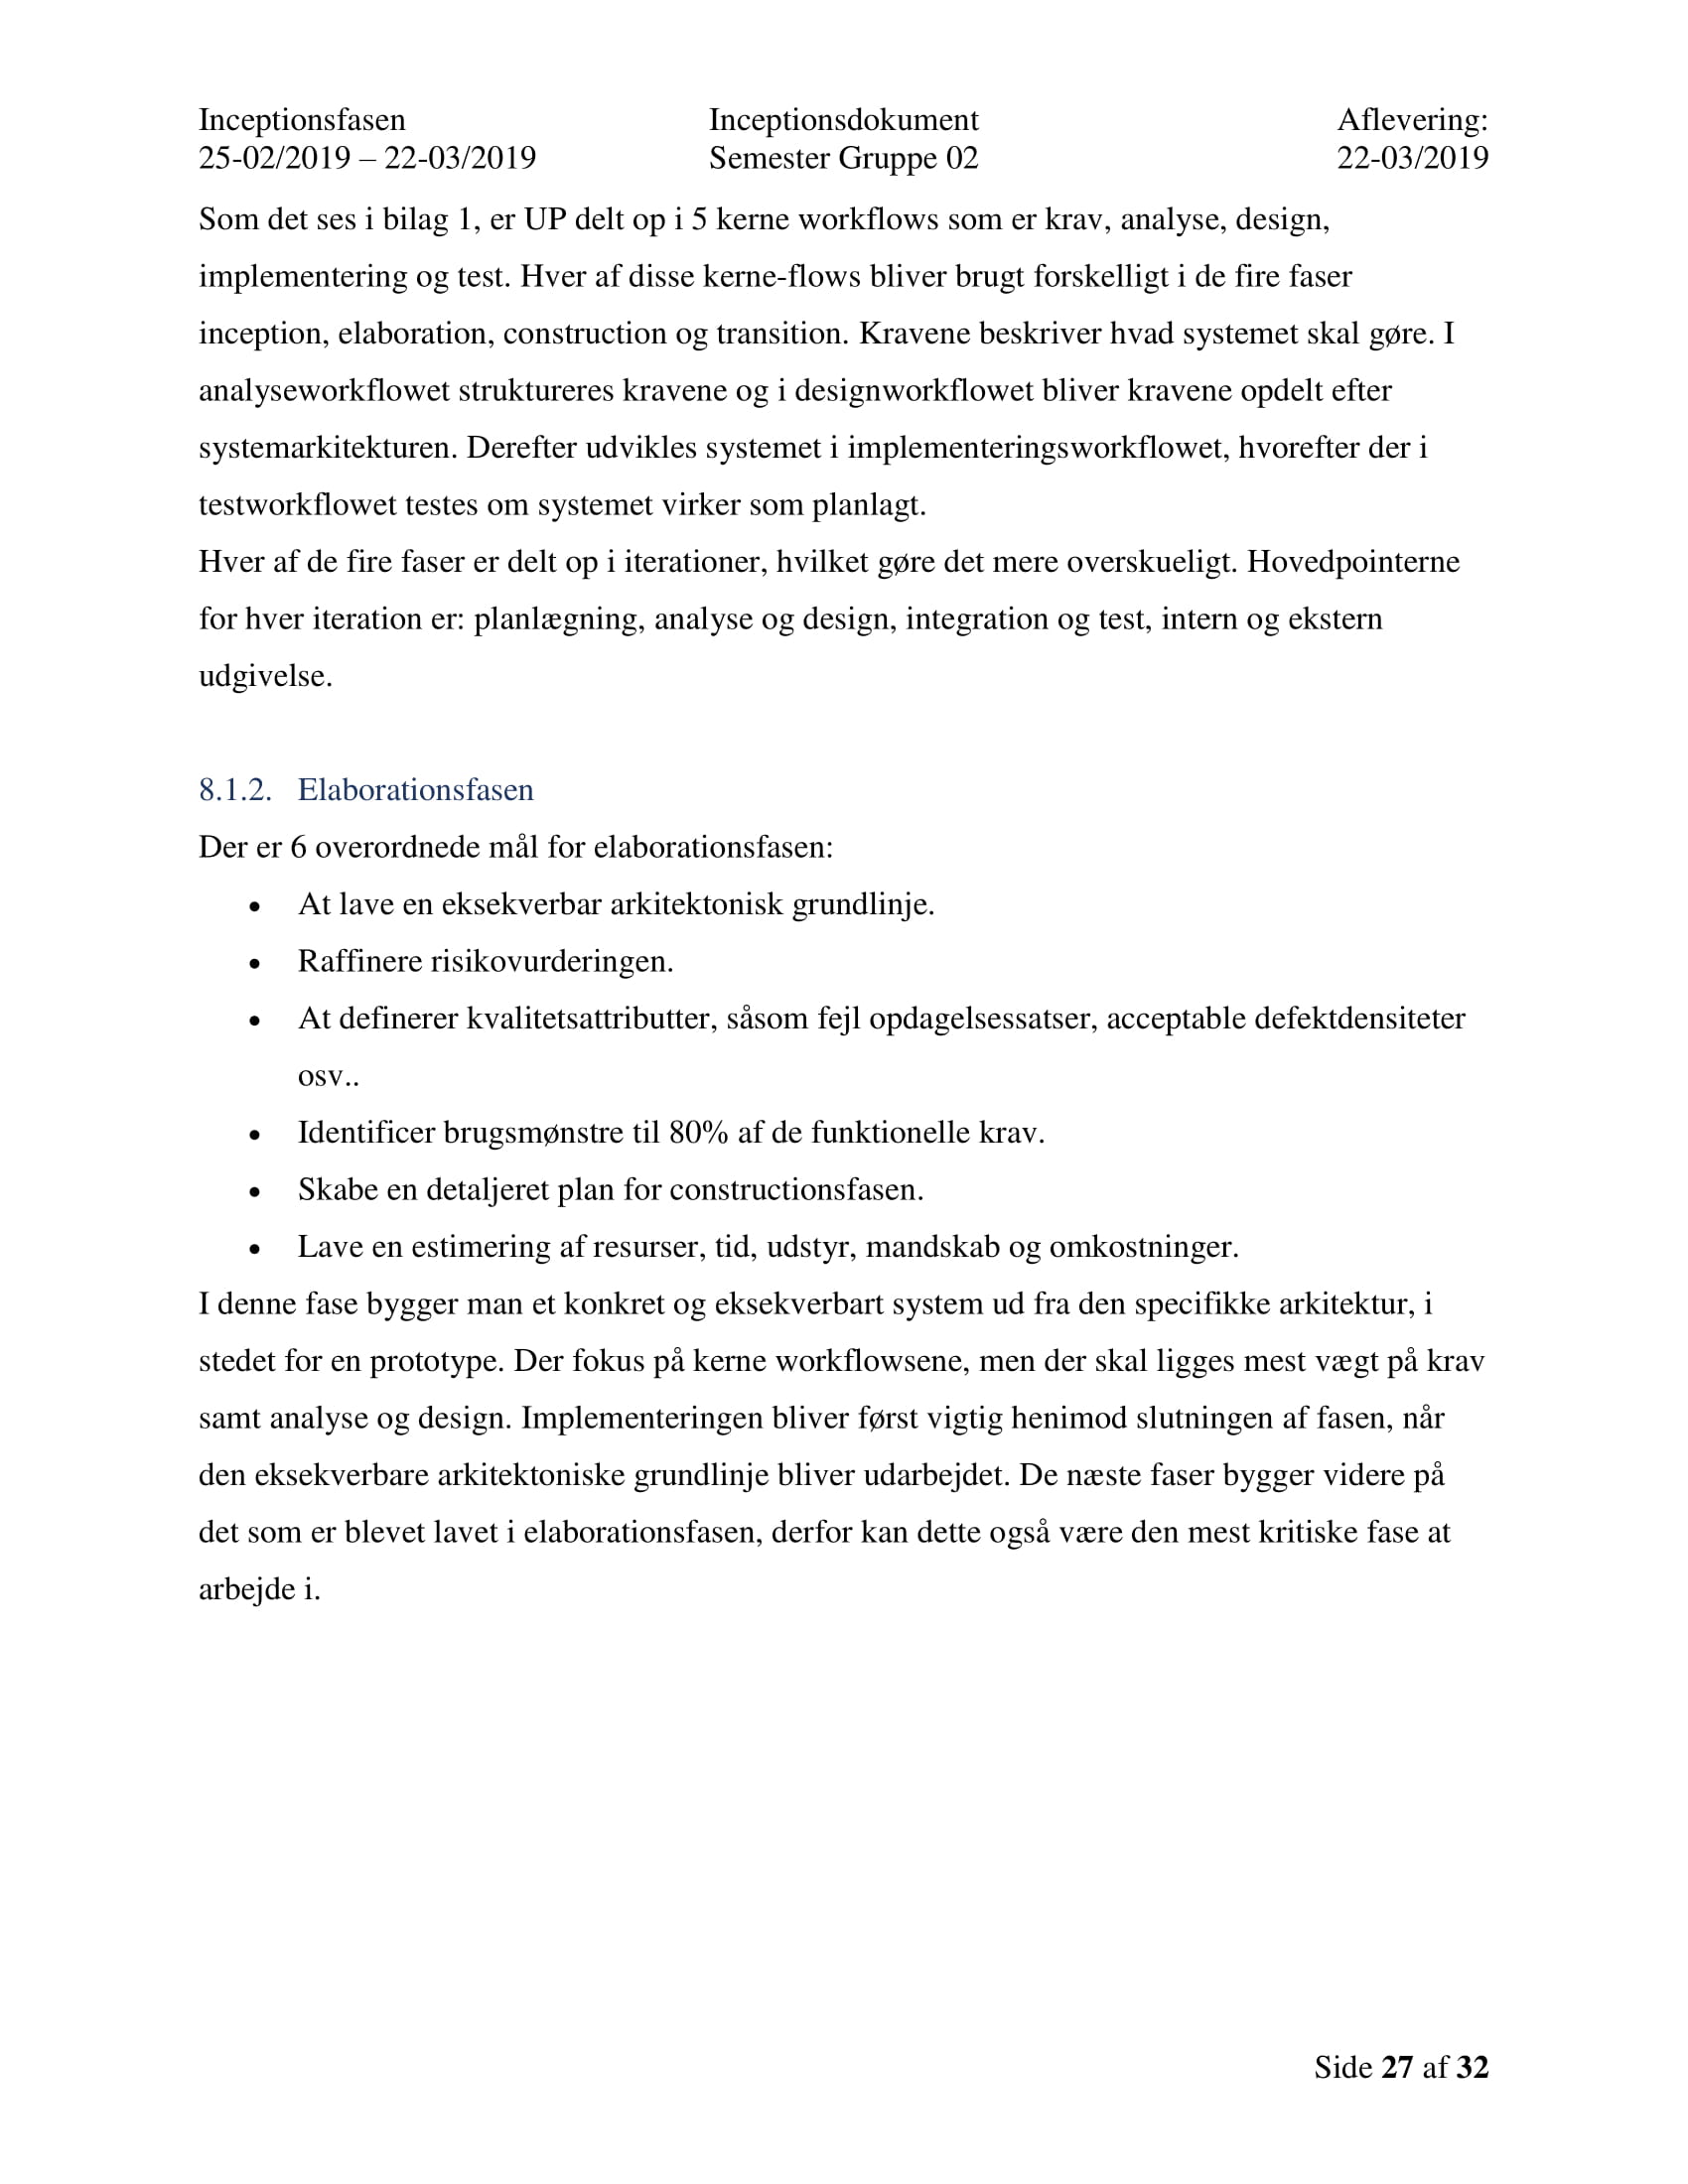
\includegraphics[scale = 0.33]{./PNG/Inceptions/Gruppe 02 + InceptionsDokument-28.jpg} 
\end{figure}

\begin{figure}[hb]
  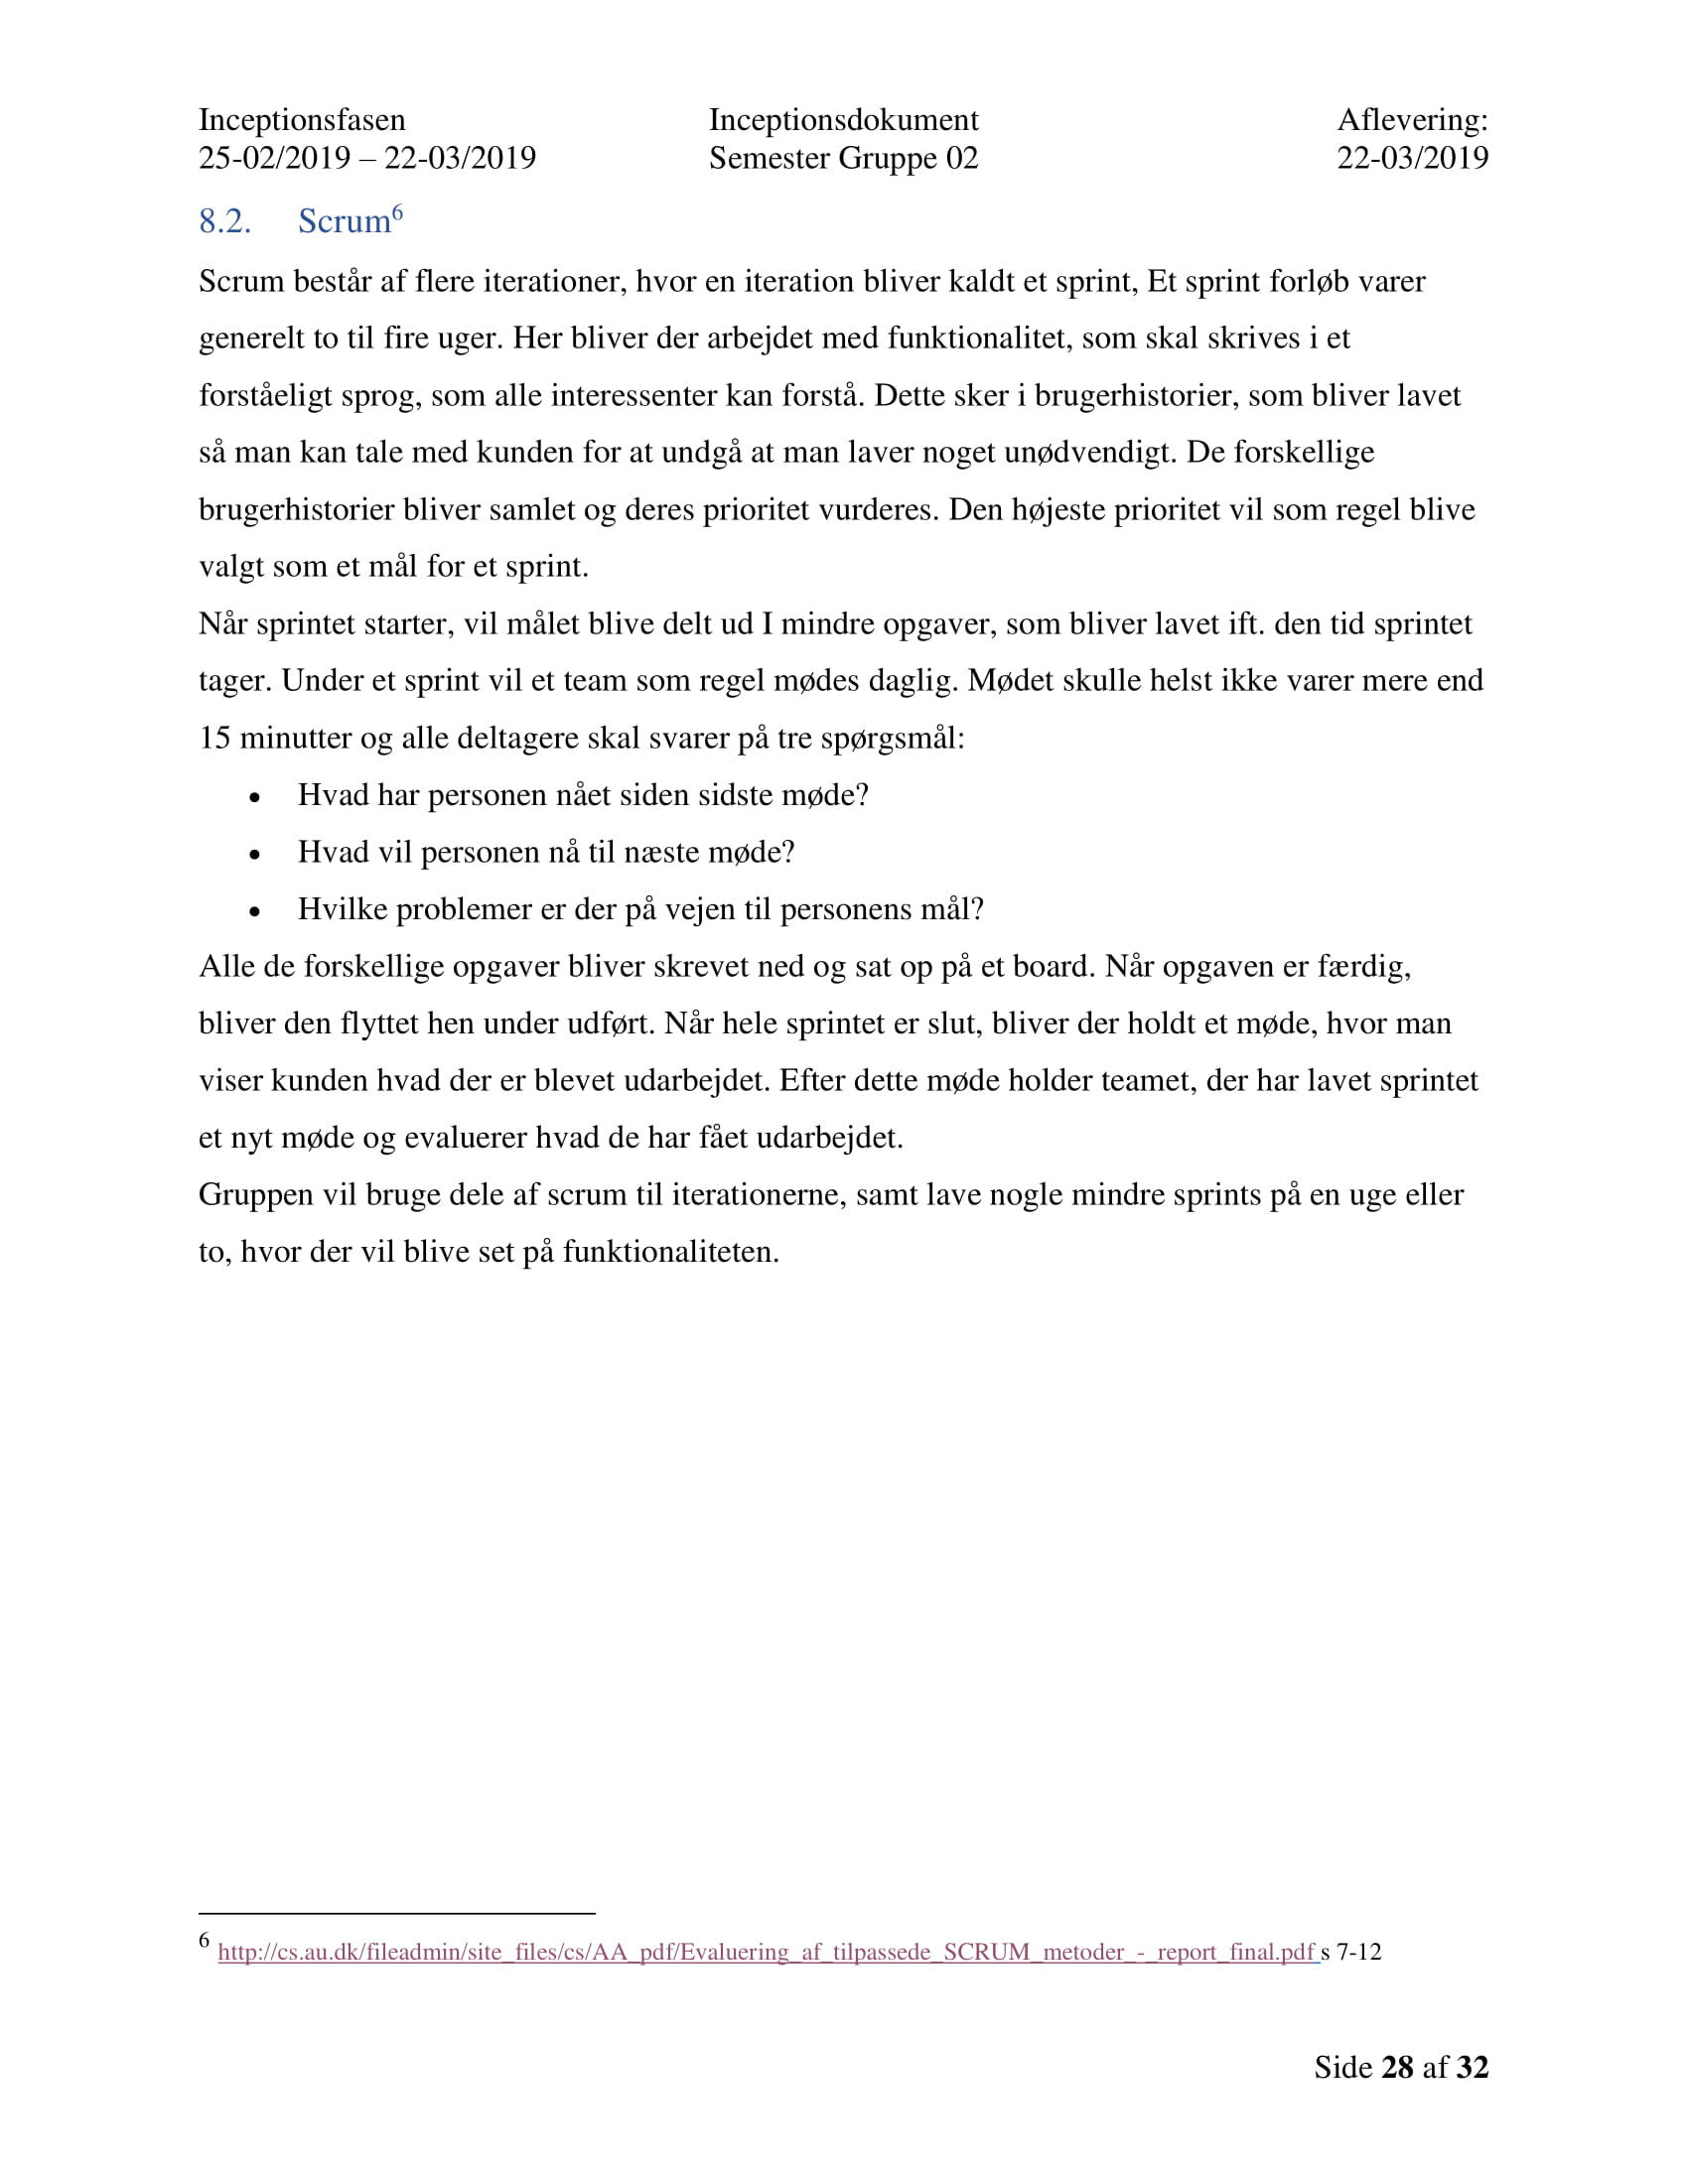
\includegraphics[scale = 0.33]{./PNG/Inceptions/Gruppe 02 + InceptionsDokument-29.jpg} 
\end{figure}

\begin{figure}[hb]
  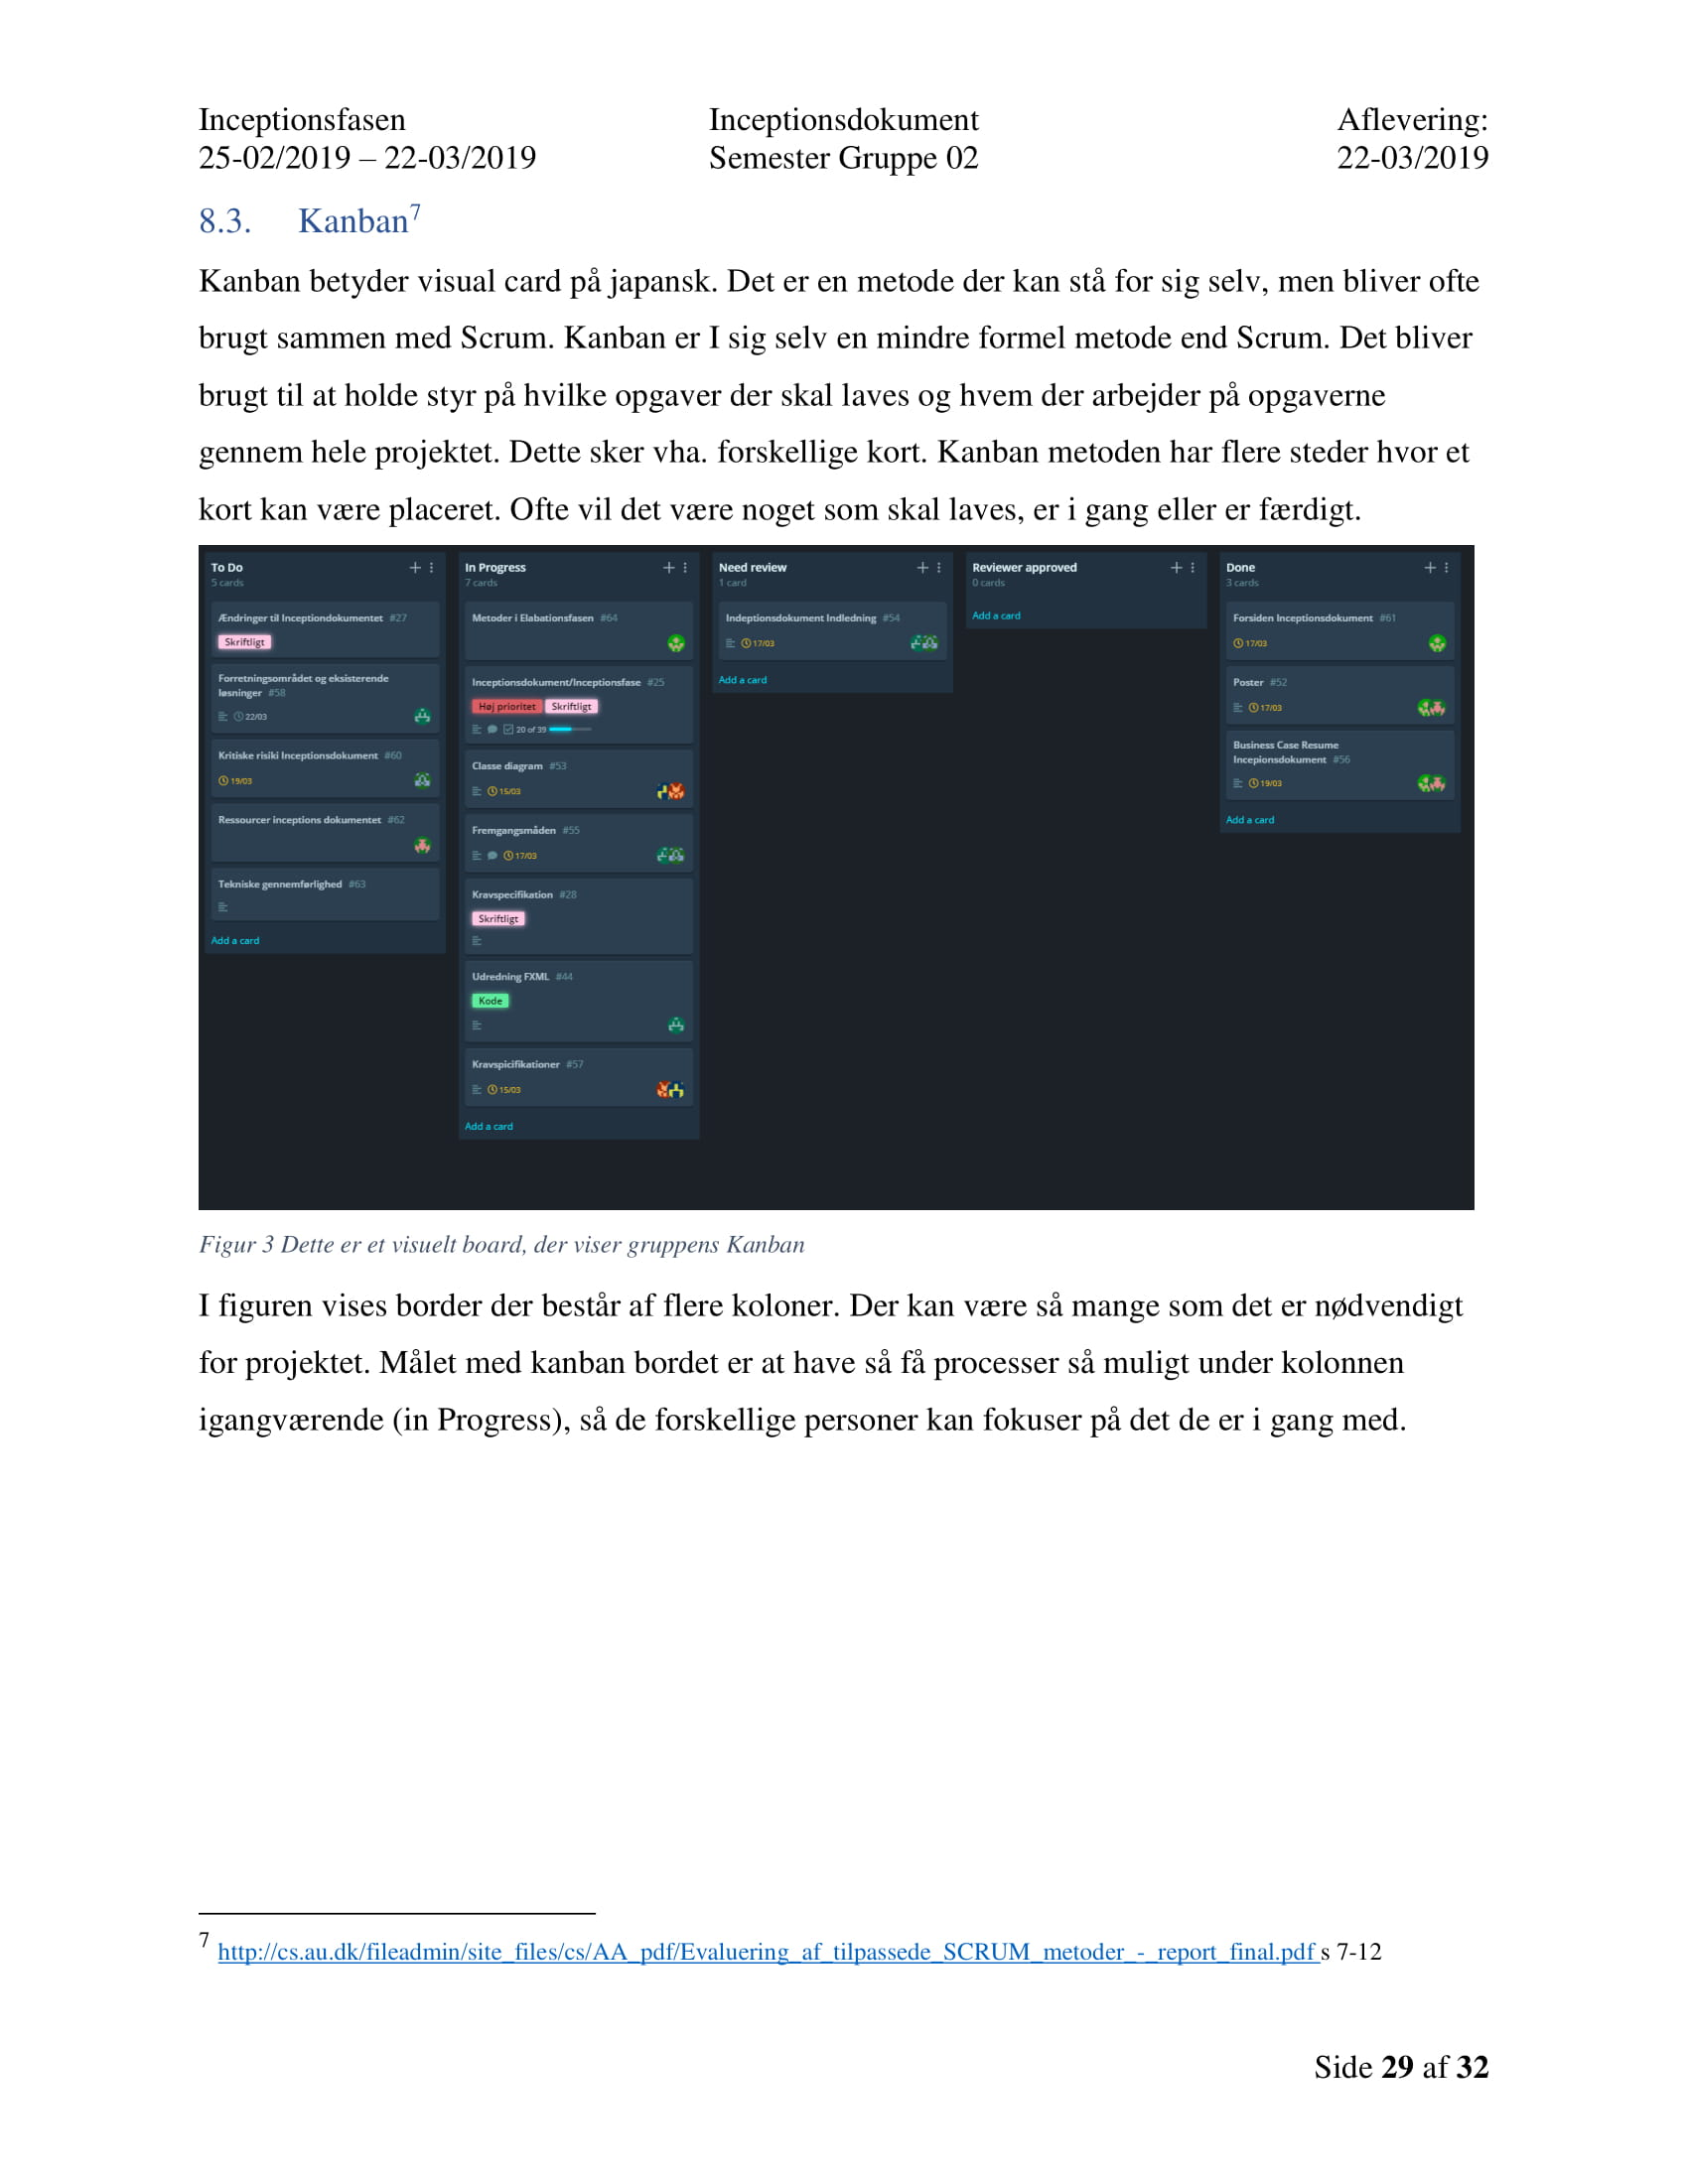
\includegraphics[scale = 0.33]{./PNG/Inceptions/Gruppe 02 + InceptionsDokument-30.jpg} 
\end{figure}

\begin{figure}[hb]
  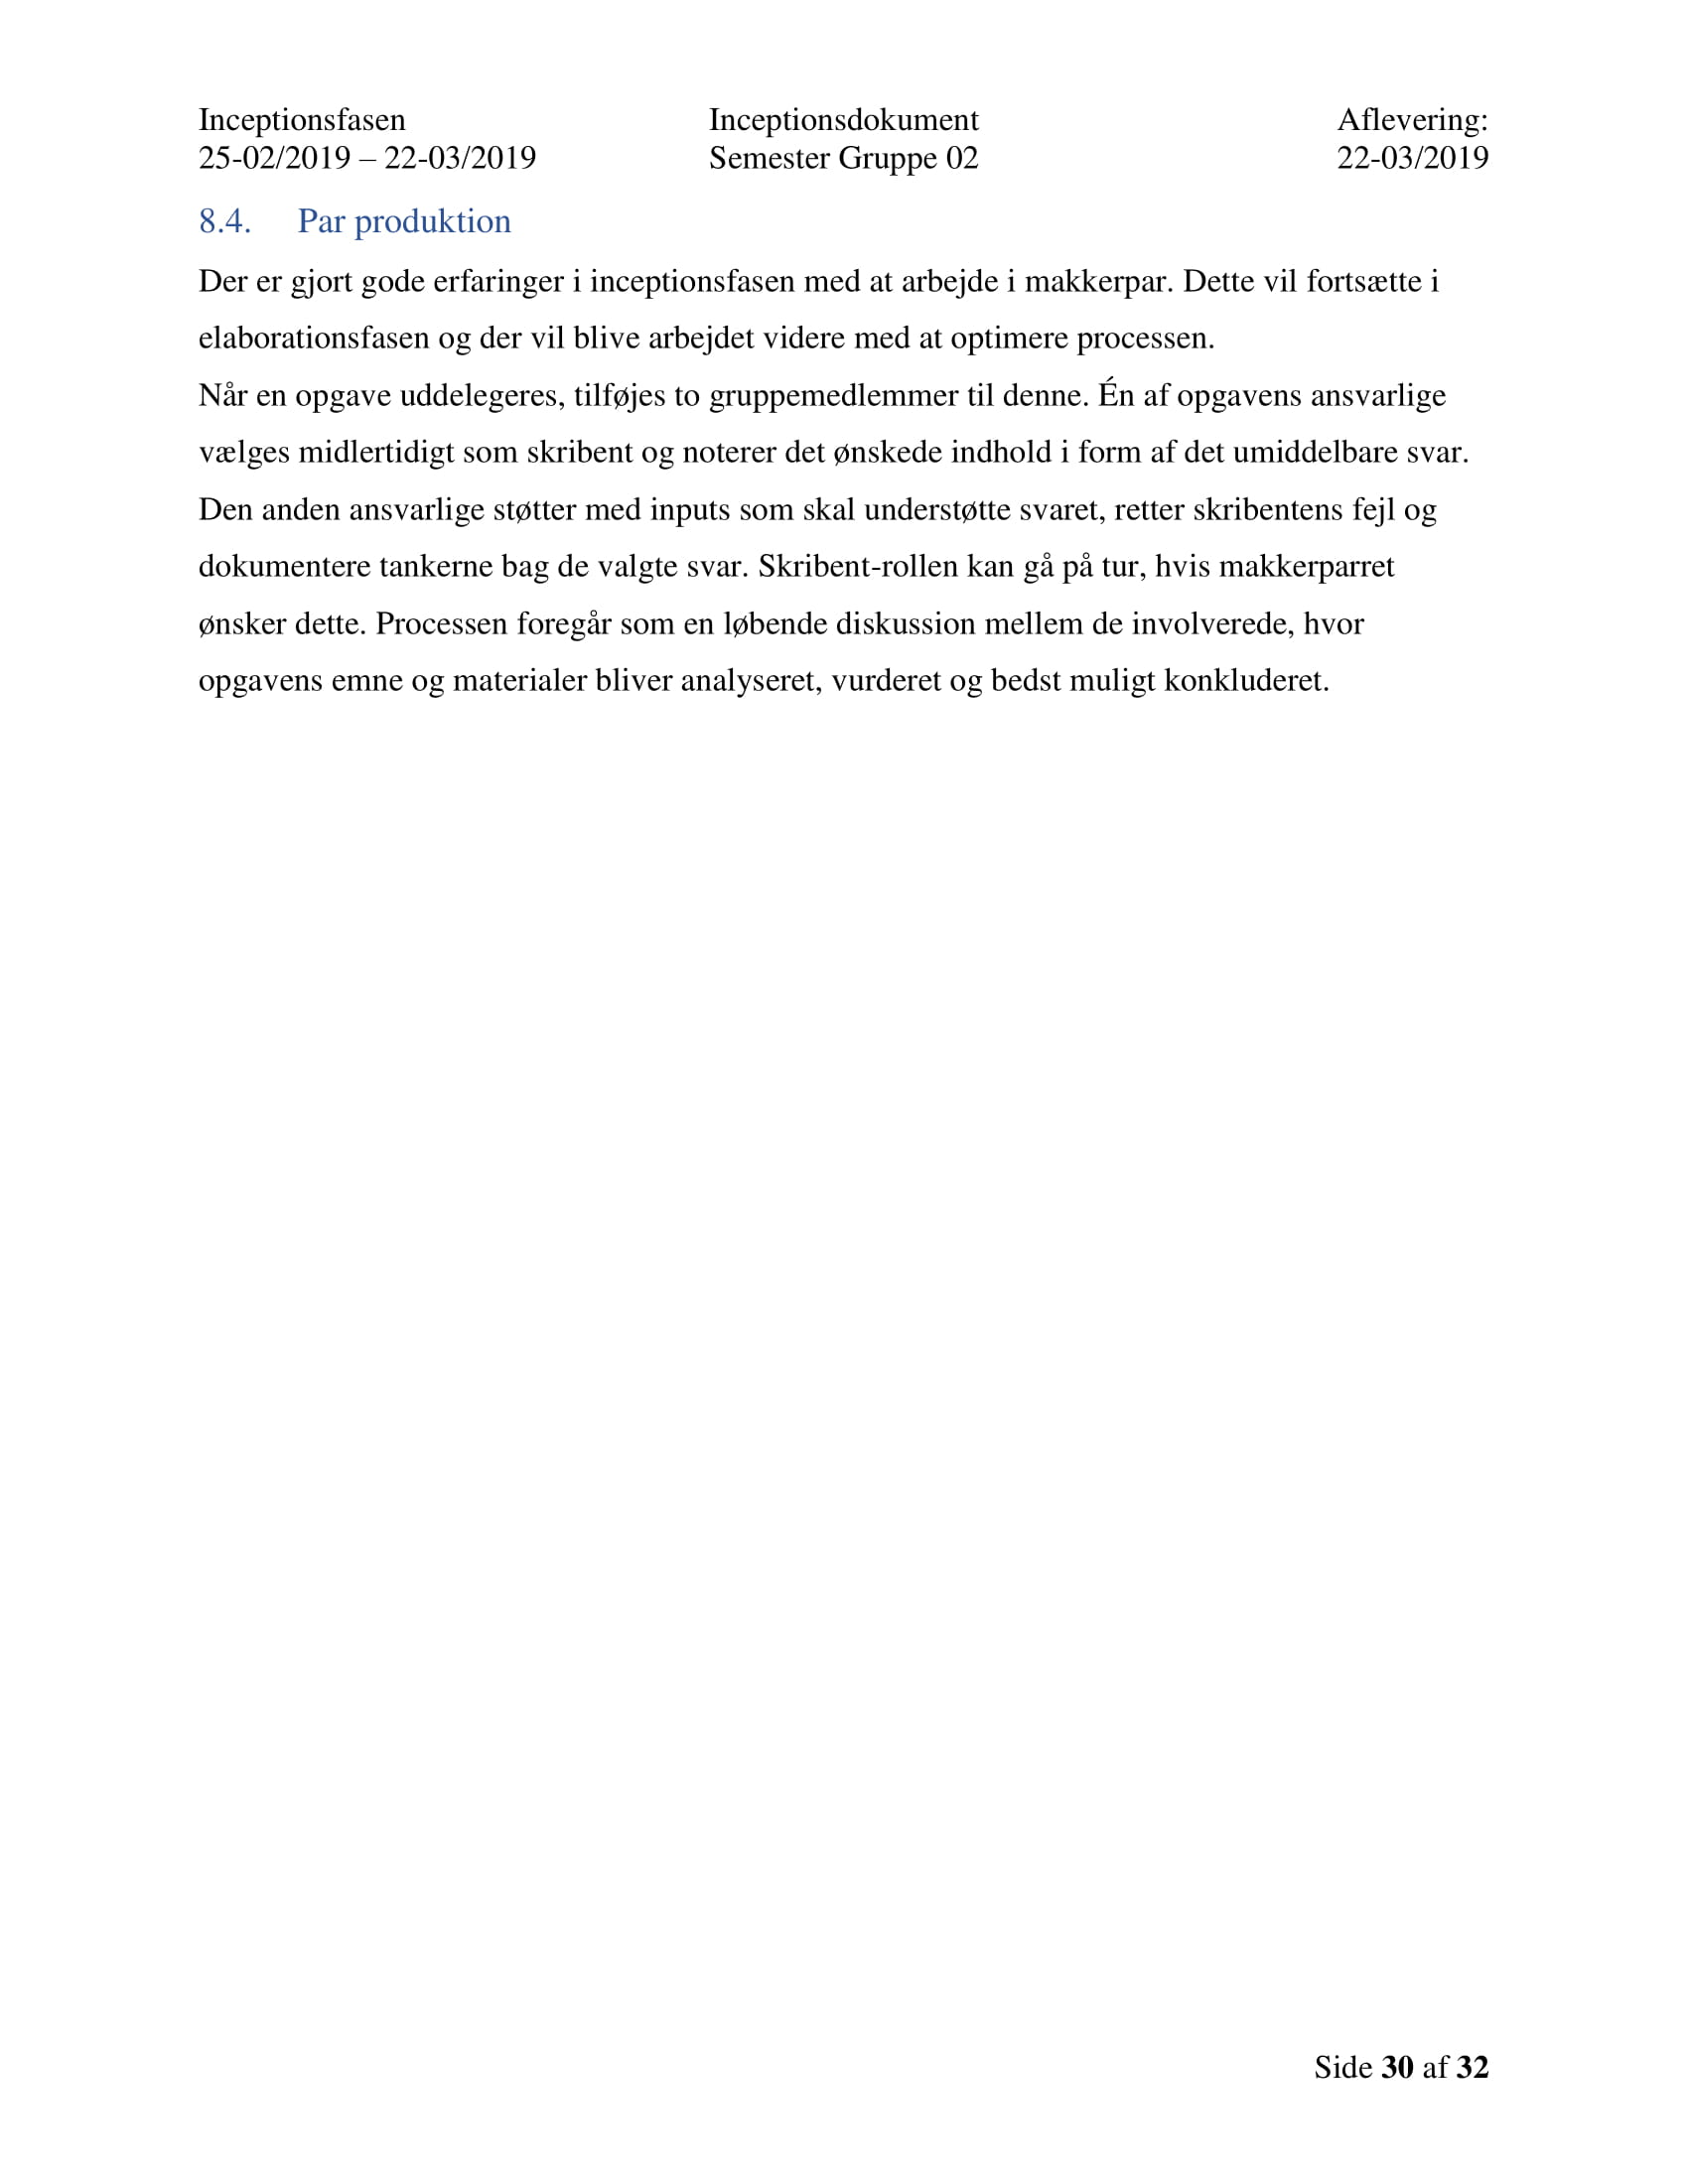
\includegraphics[scale = 0.33]{./PNG/Inceptions/Gruppe 02 + InceptionsDokument-31.jpg} 
\end{figure}

\begin{landscape}
\begin{figure}[hb]
  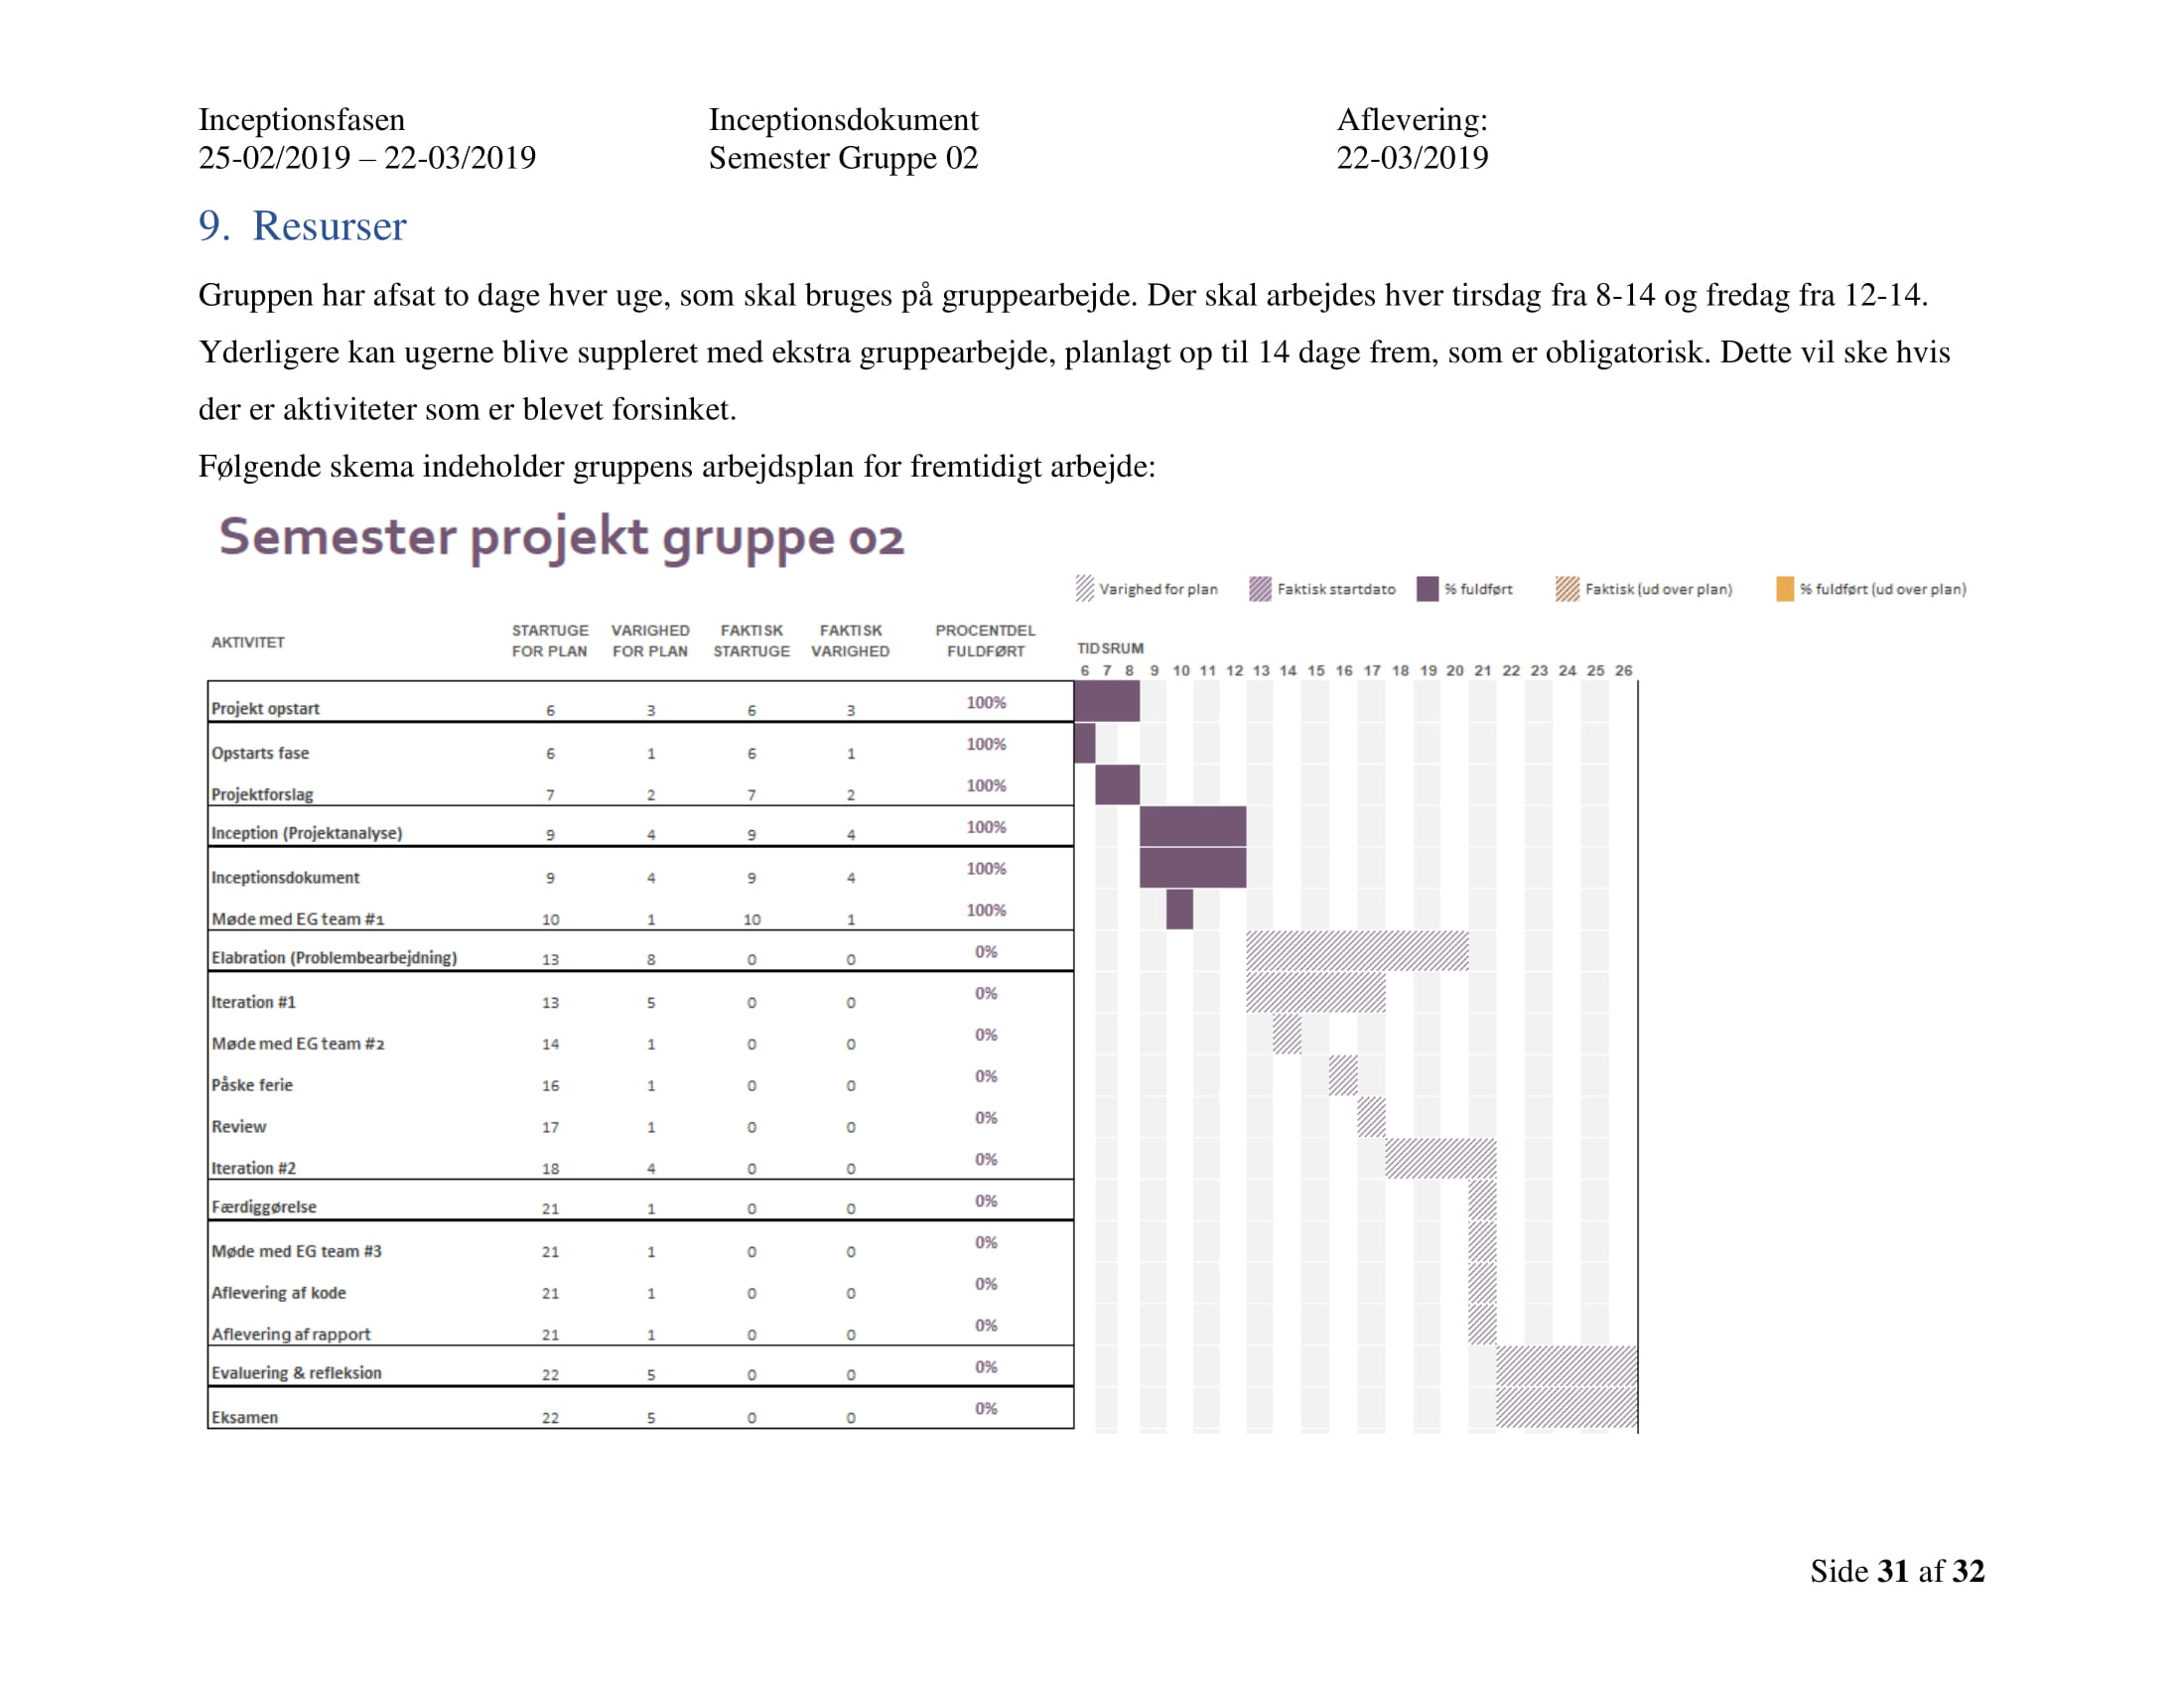
\includegraphics[scale = 0.33]{./PNG/Inceptions/Gruppe 02 + InceptionsDokument-32.jpg} 
\end{figure}
\end{landscape}

\begin{figure}[hb]
  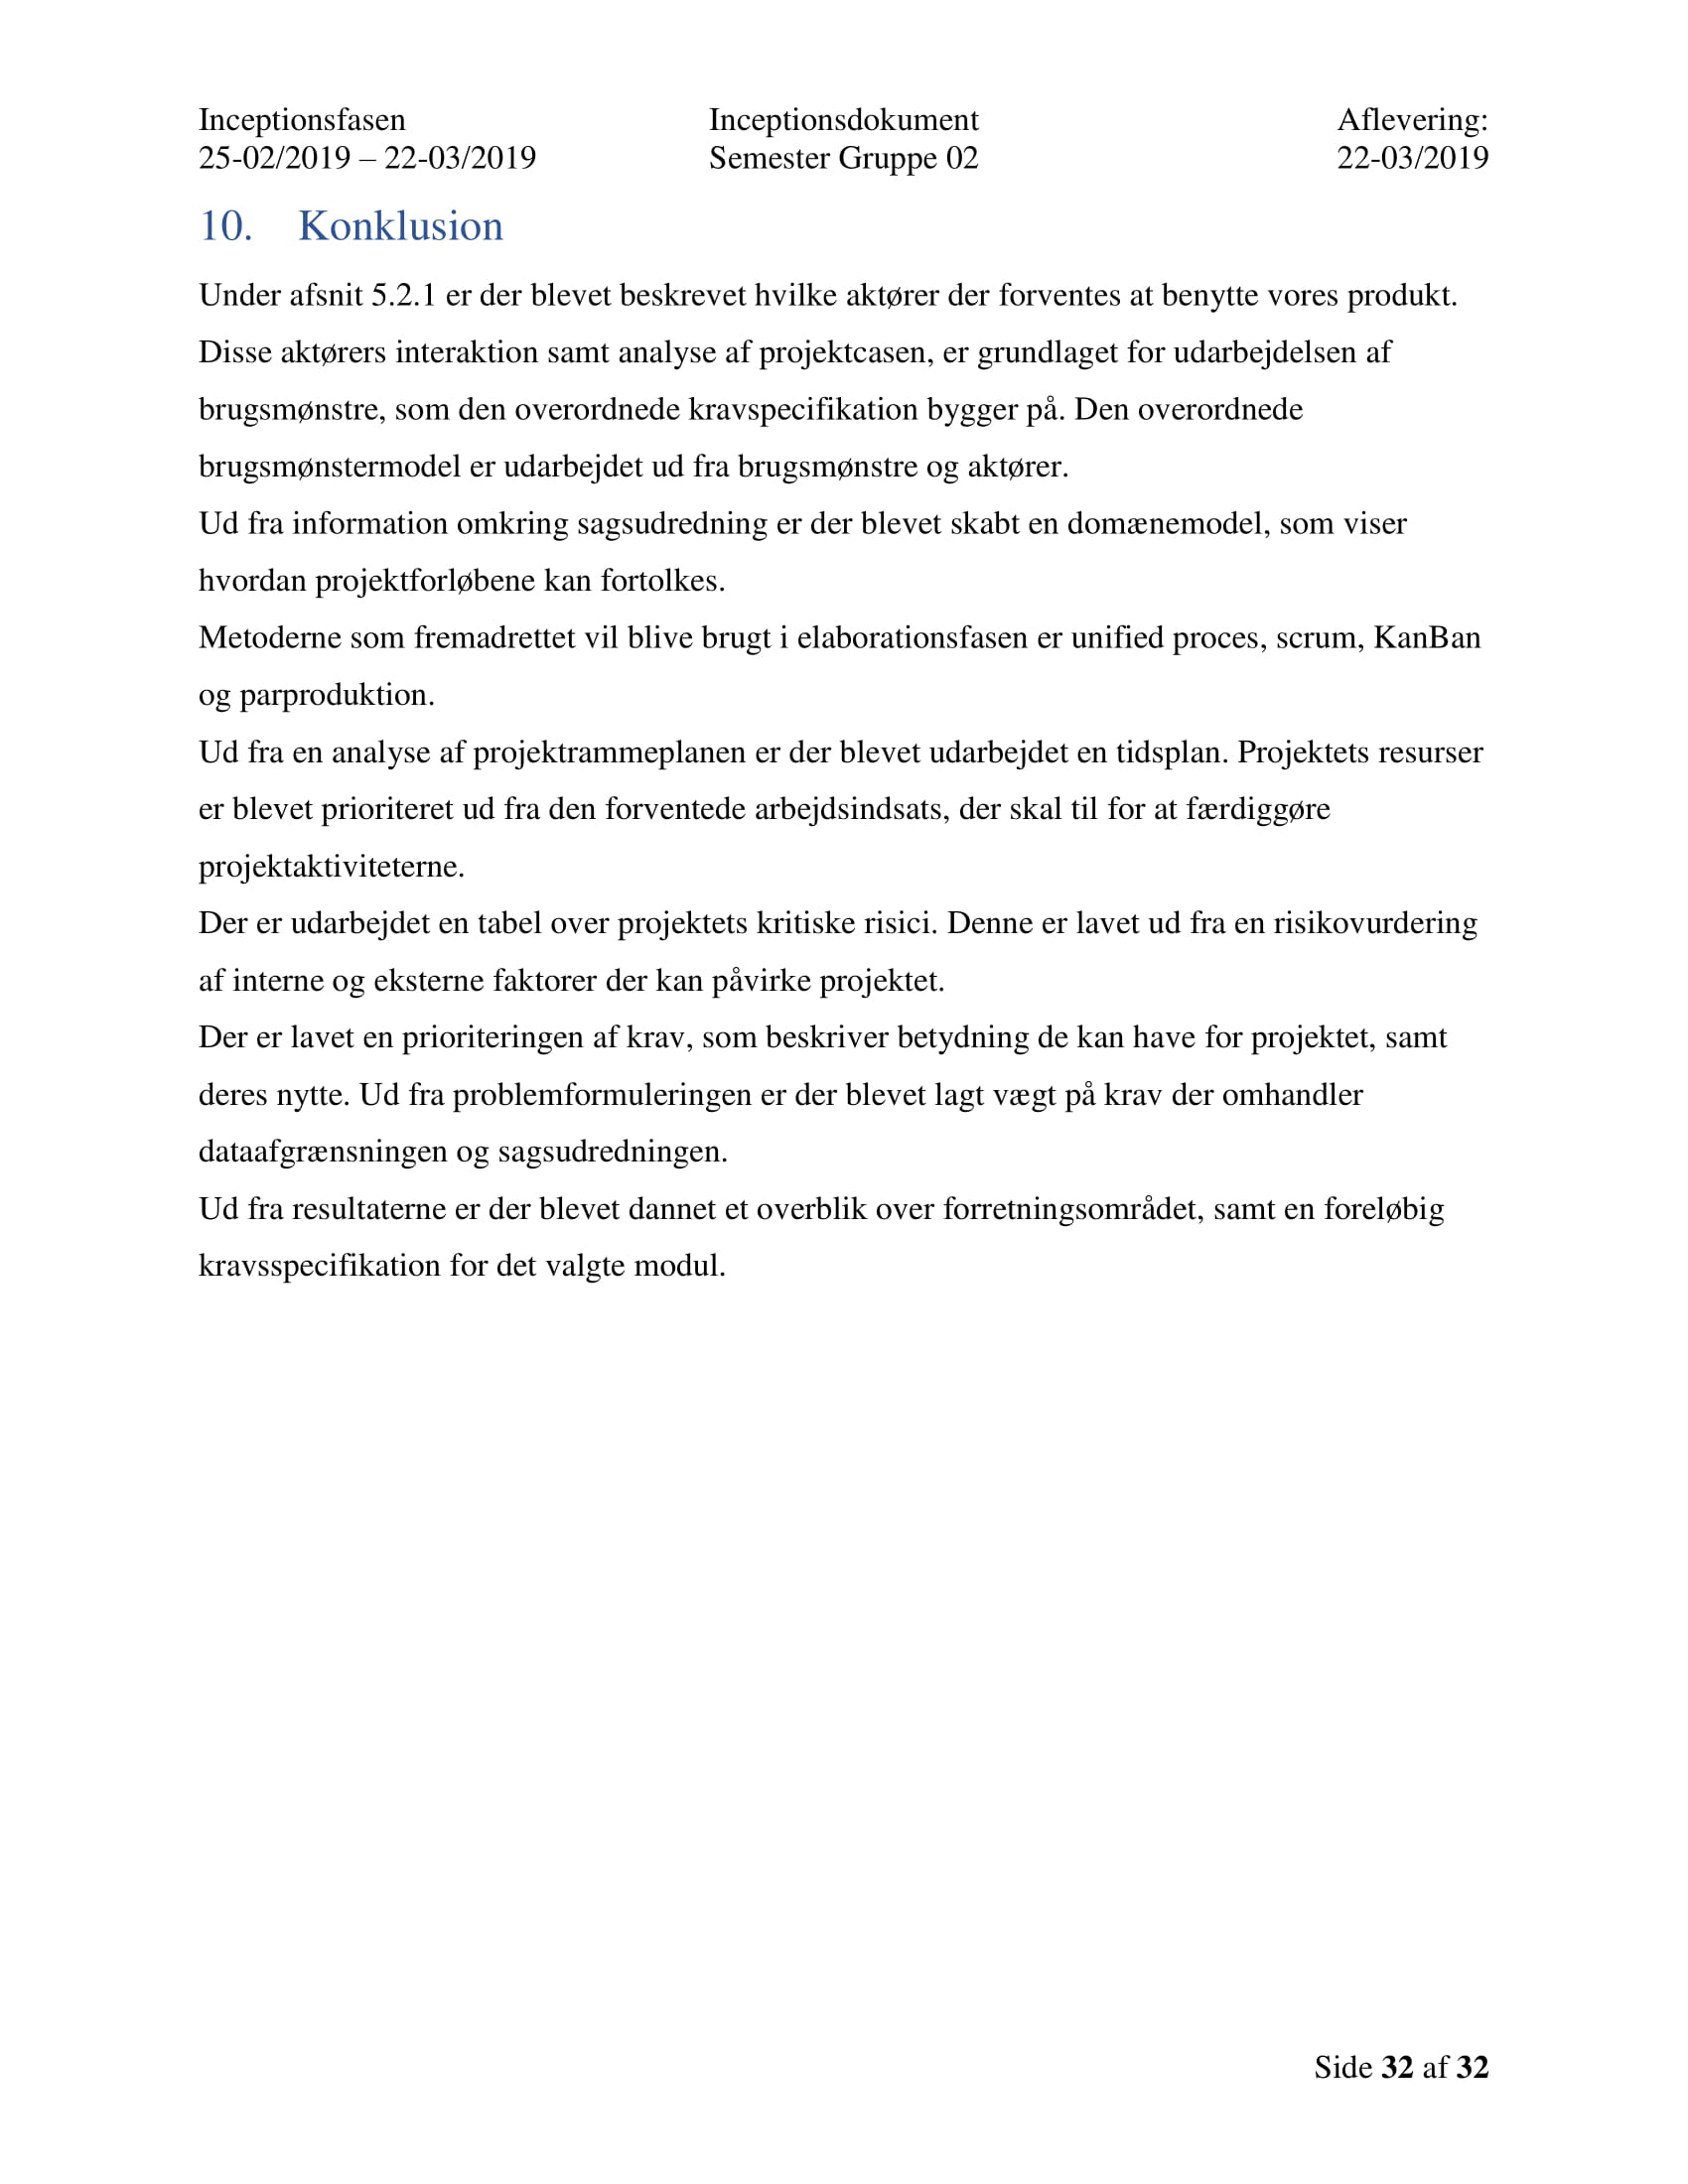
\includegraphics[scale = 0.33]{./PNG/Inceptions/Gruppe 02 + InceptionsDokument-33.jpg} 
\end{figure}

\begin{figure}[hb]
  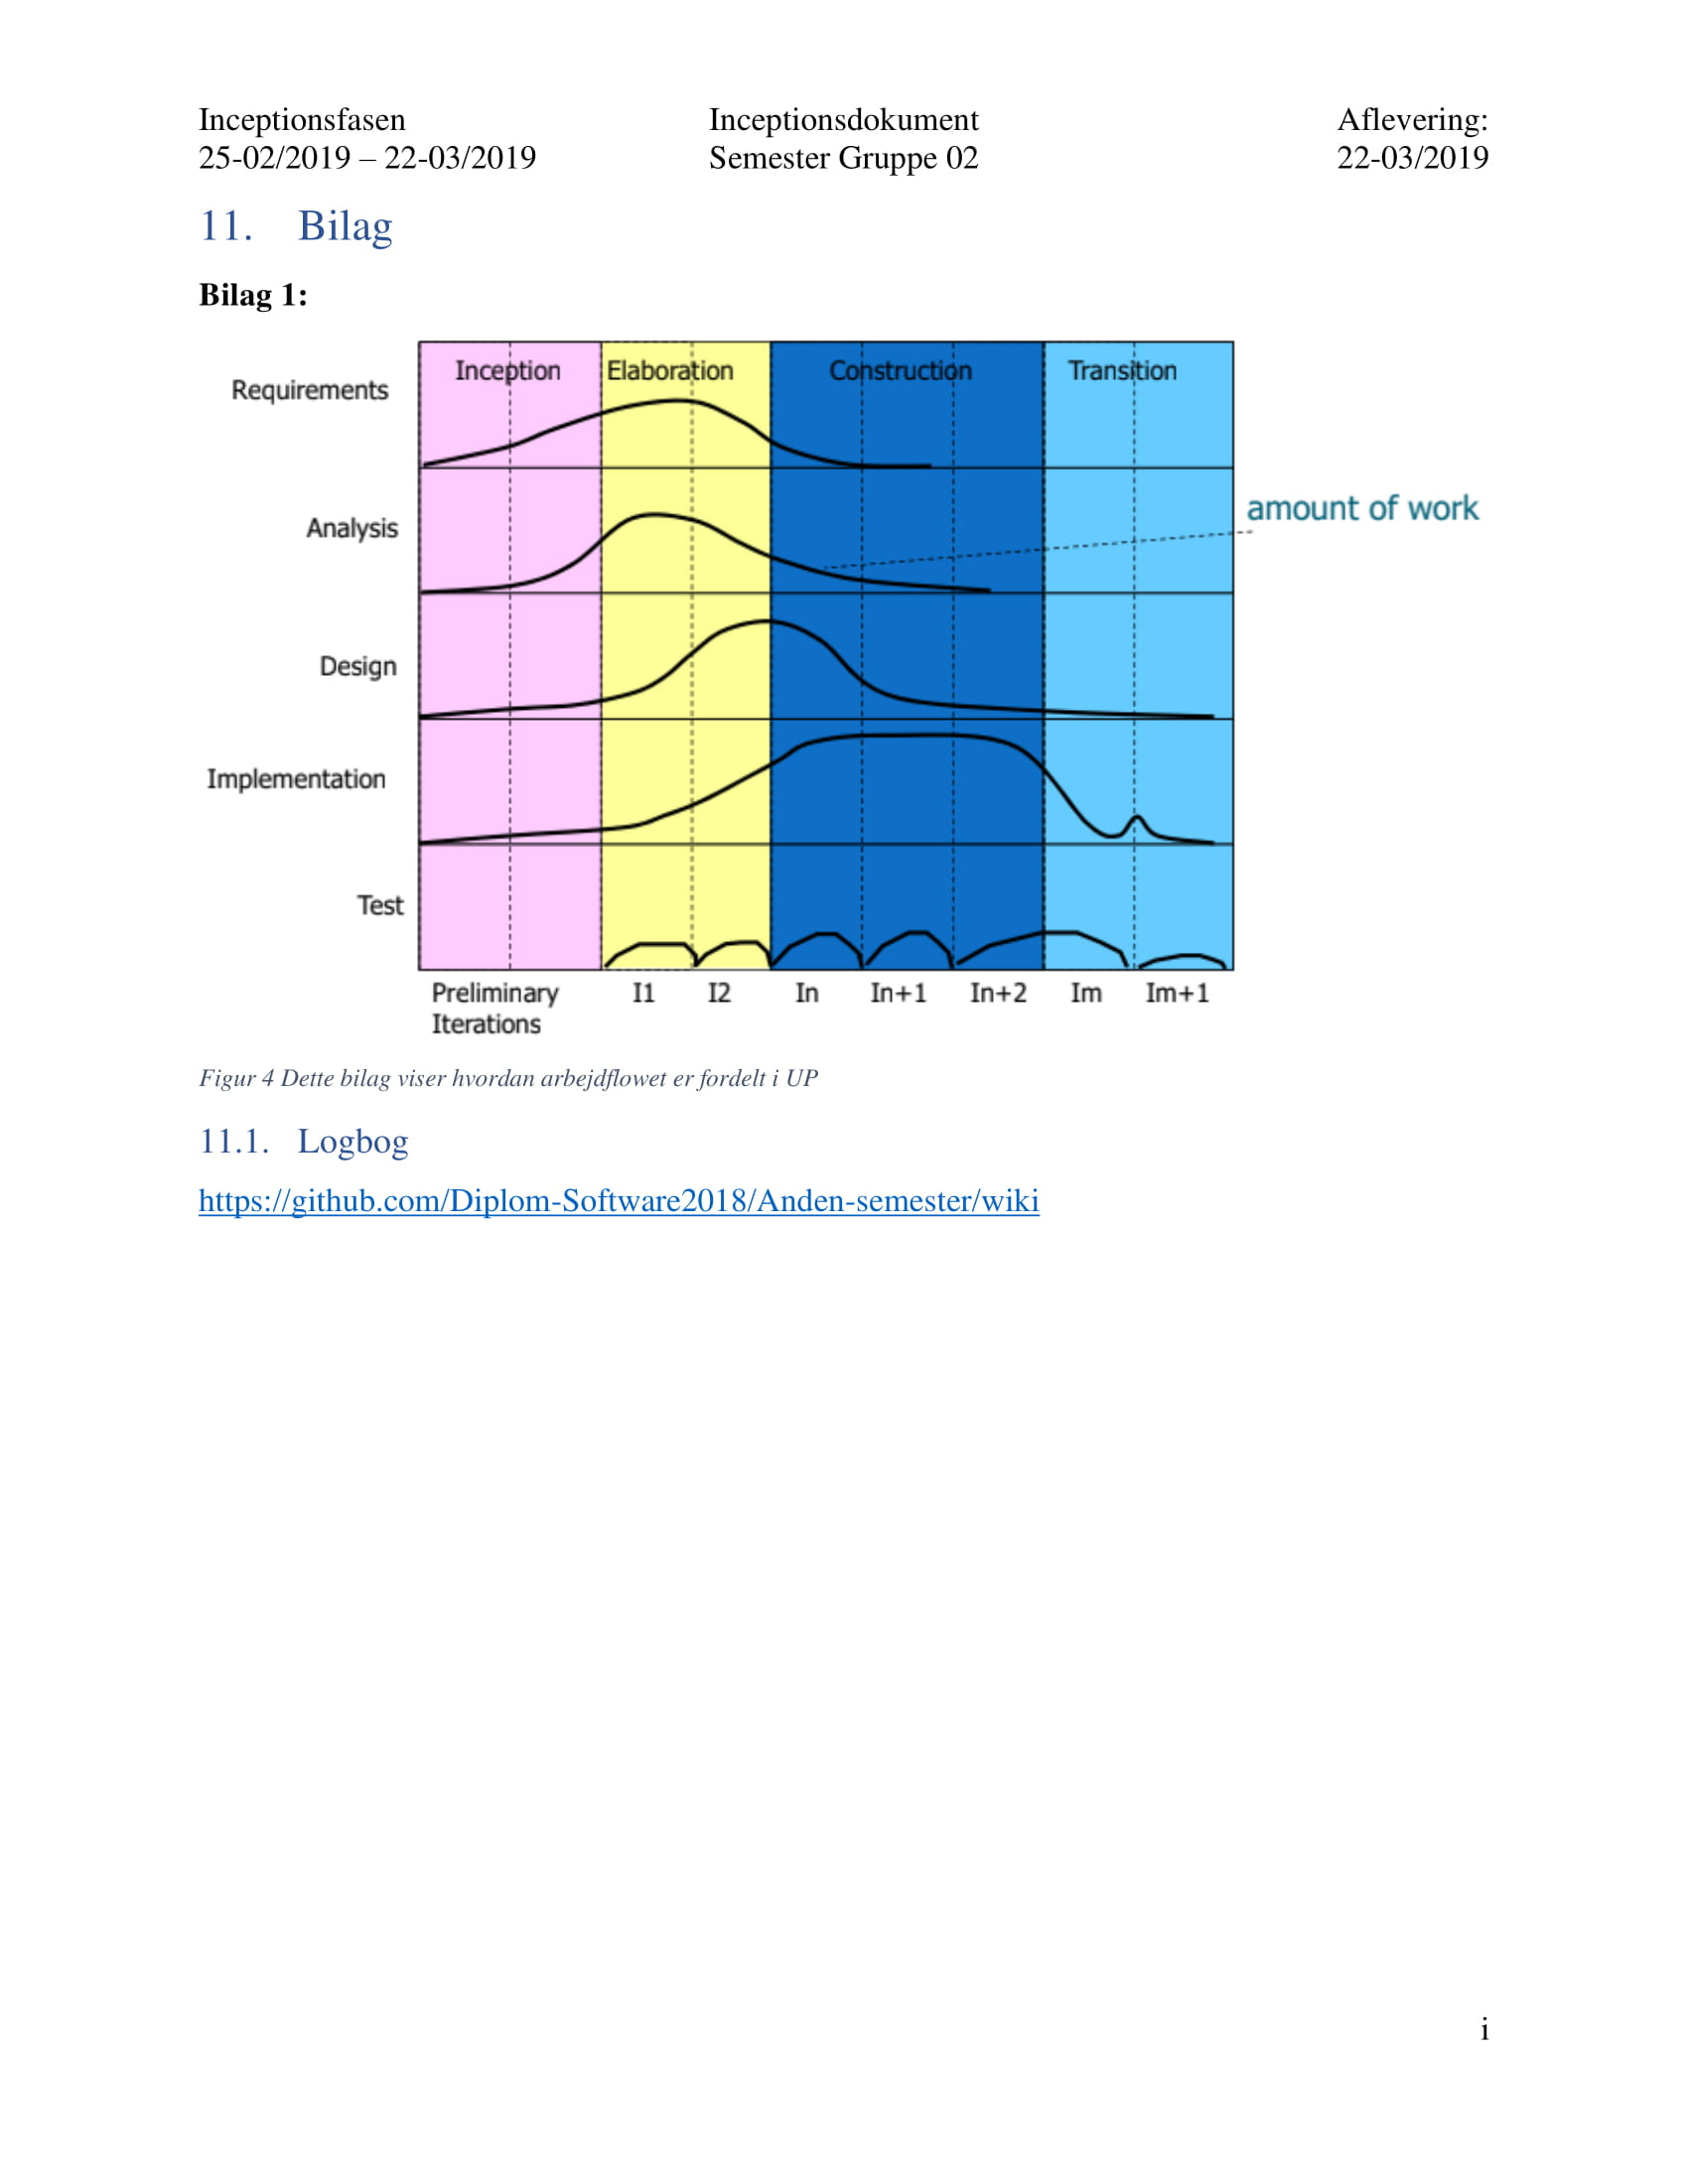
\includegraphics[scale = 0.33]{./PNG/Inceptions/Gruppe 02 + InceptionsDokument-34.jpg} 
\end{figure}

\begin{figure}[hb]
  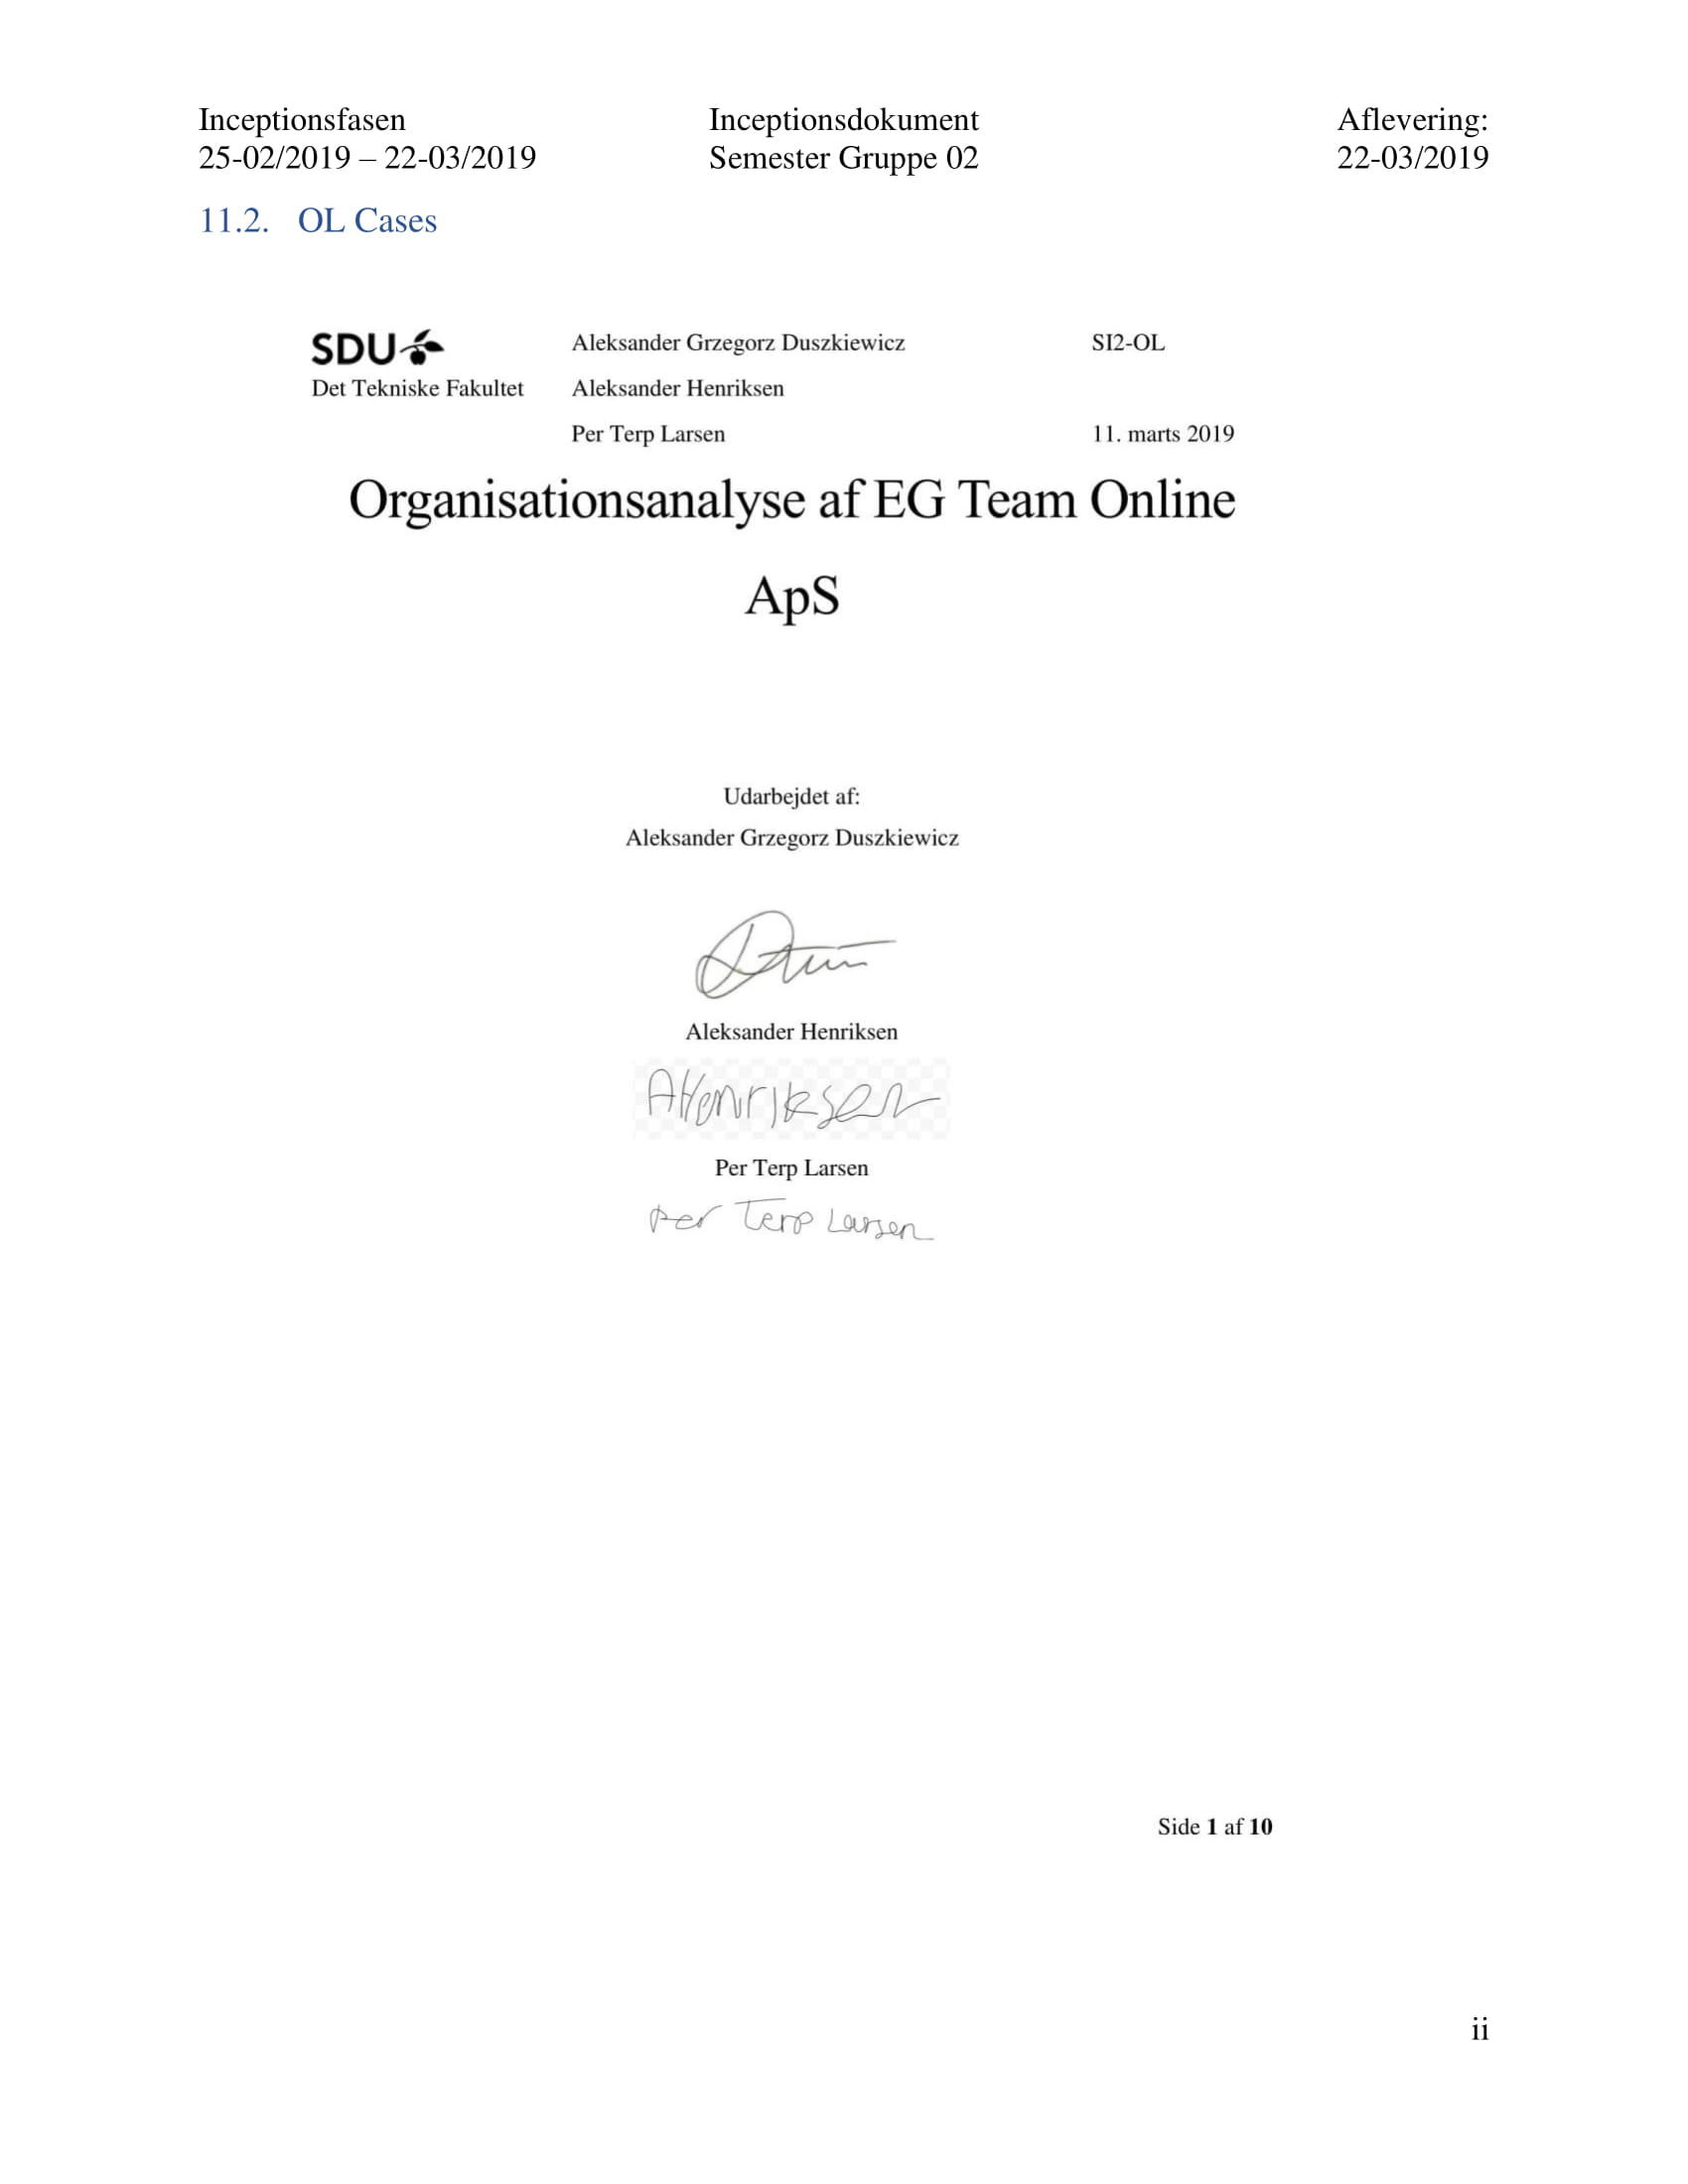
\includegraphics[scale = 0.33]{./PNG/Inceptions/Gruppe 02 + InceptionsDokument-35.jpg} 
\end{figure}

\begin{figure}[hb]
  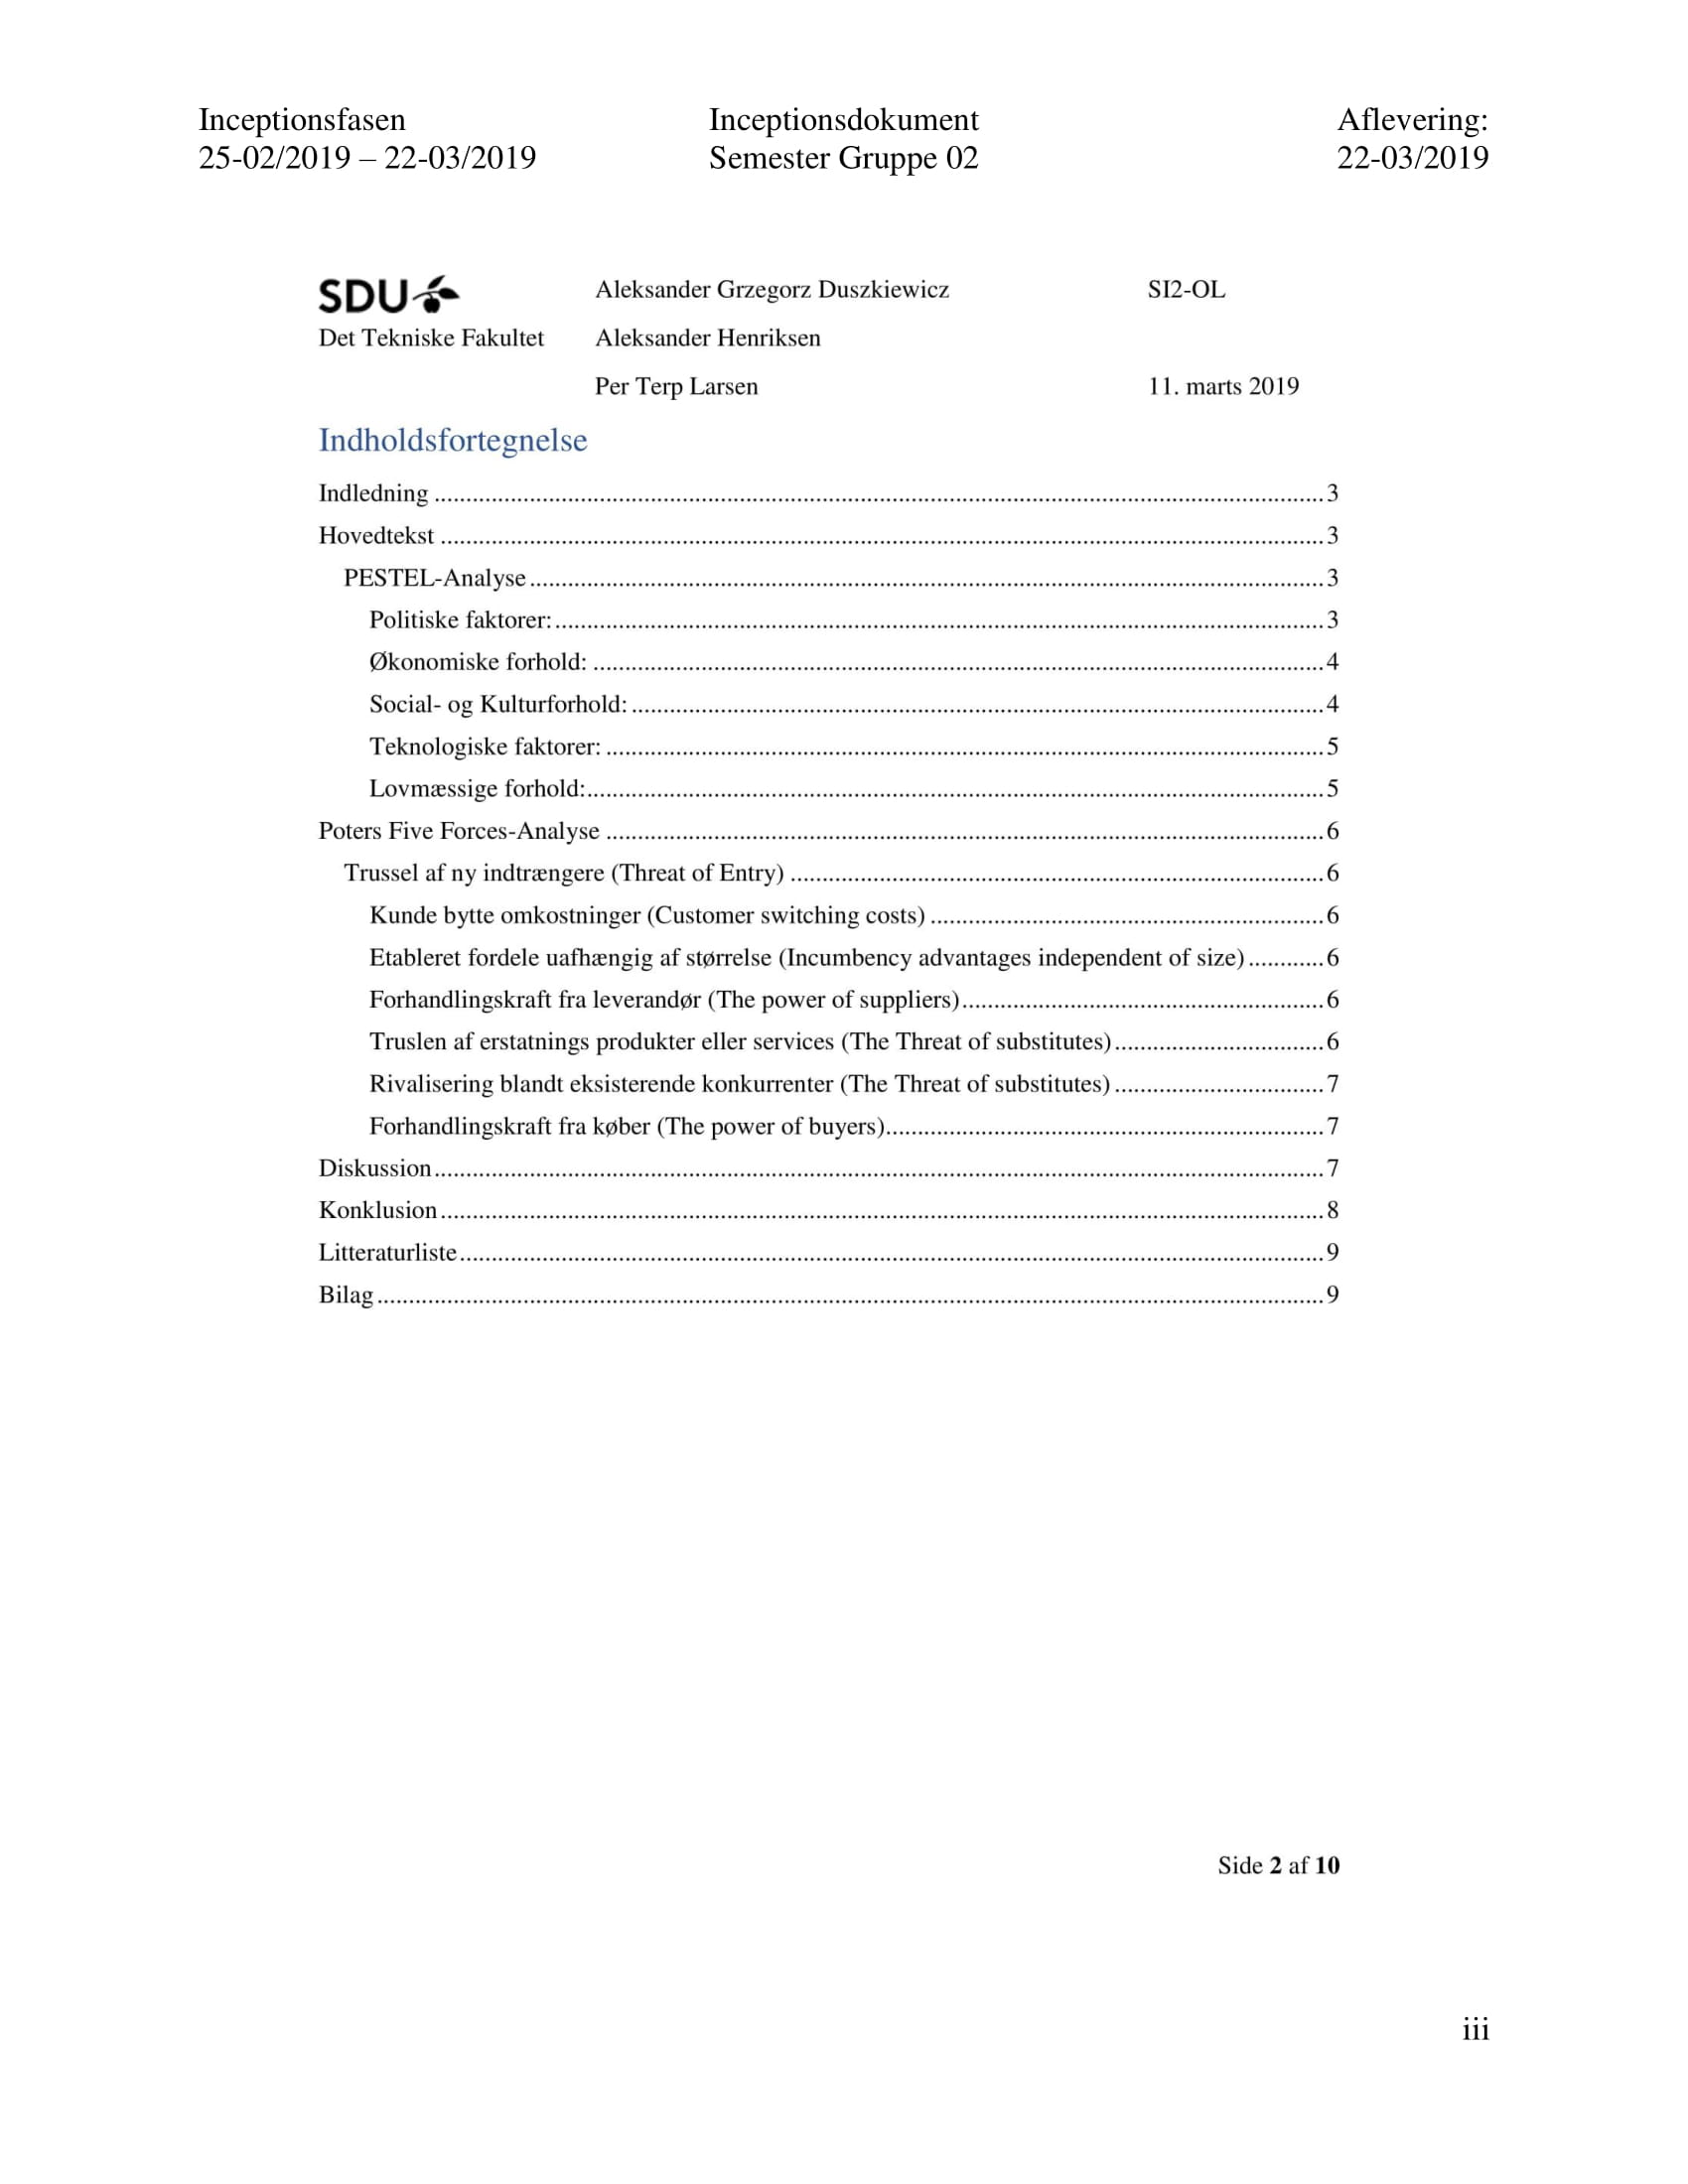
\includegraphics[scale = 0.33]{./PNG/Inceptions/Gruppe 02 + InceptionsDokument-36.jpg} 
\end{figure}

\begin{figure}[hb]
  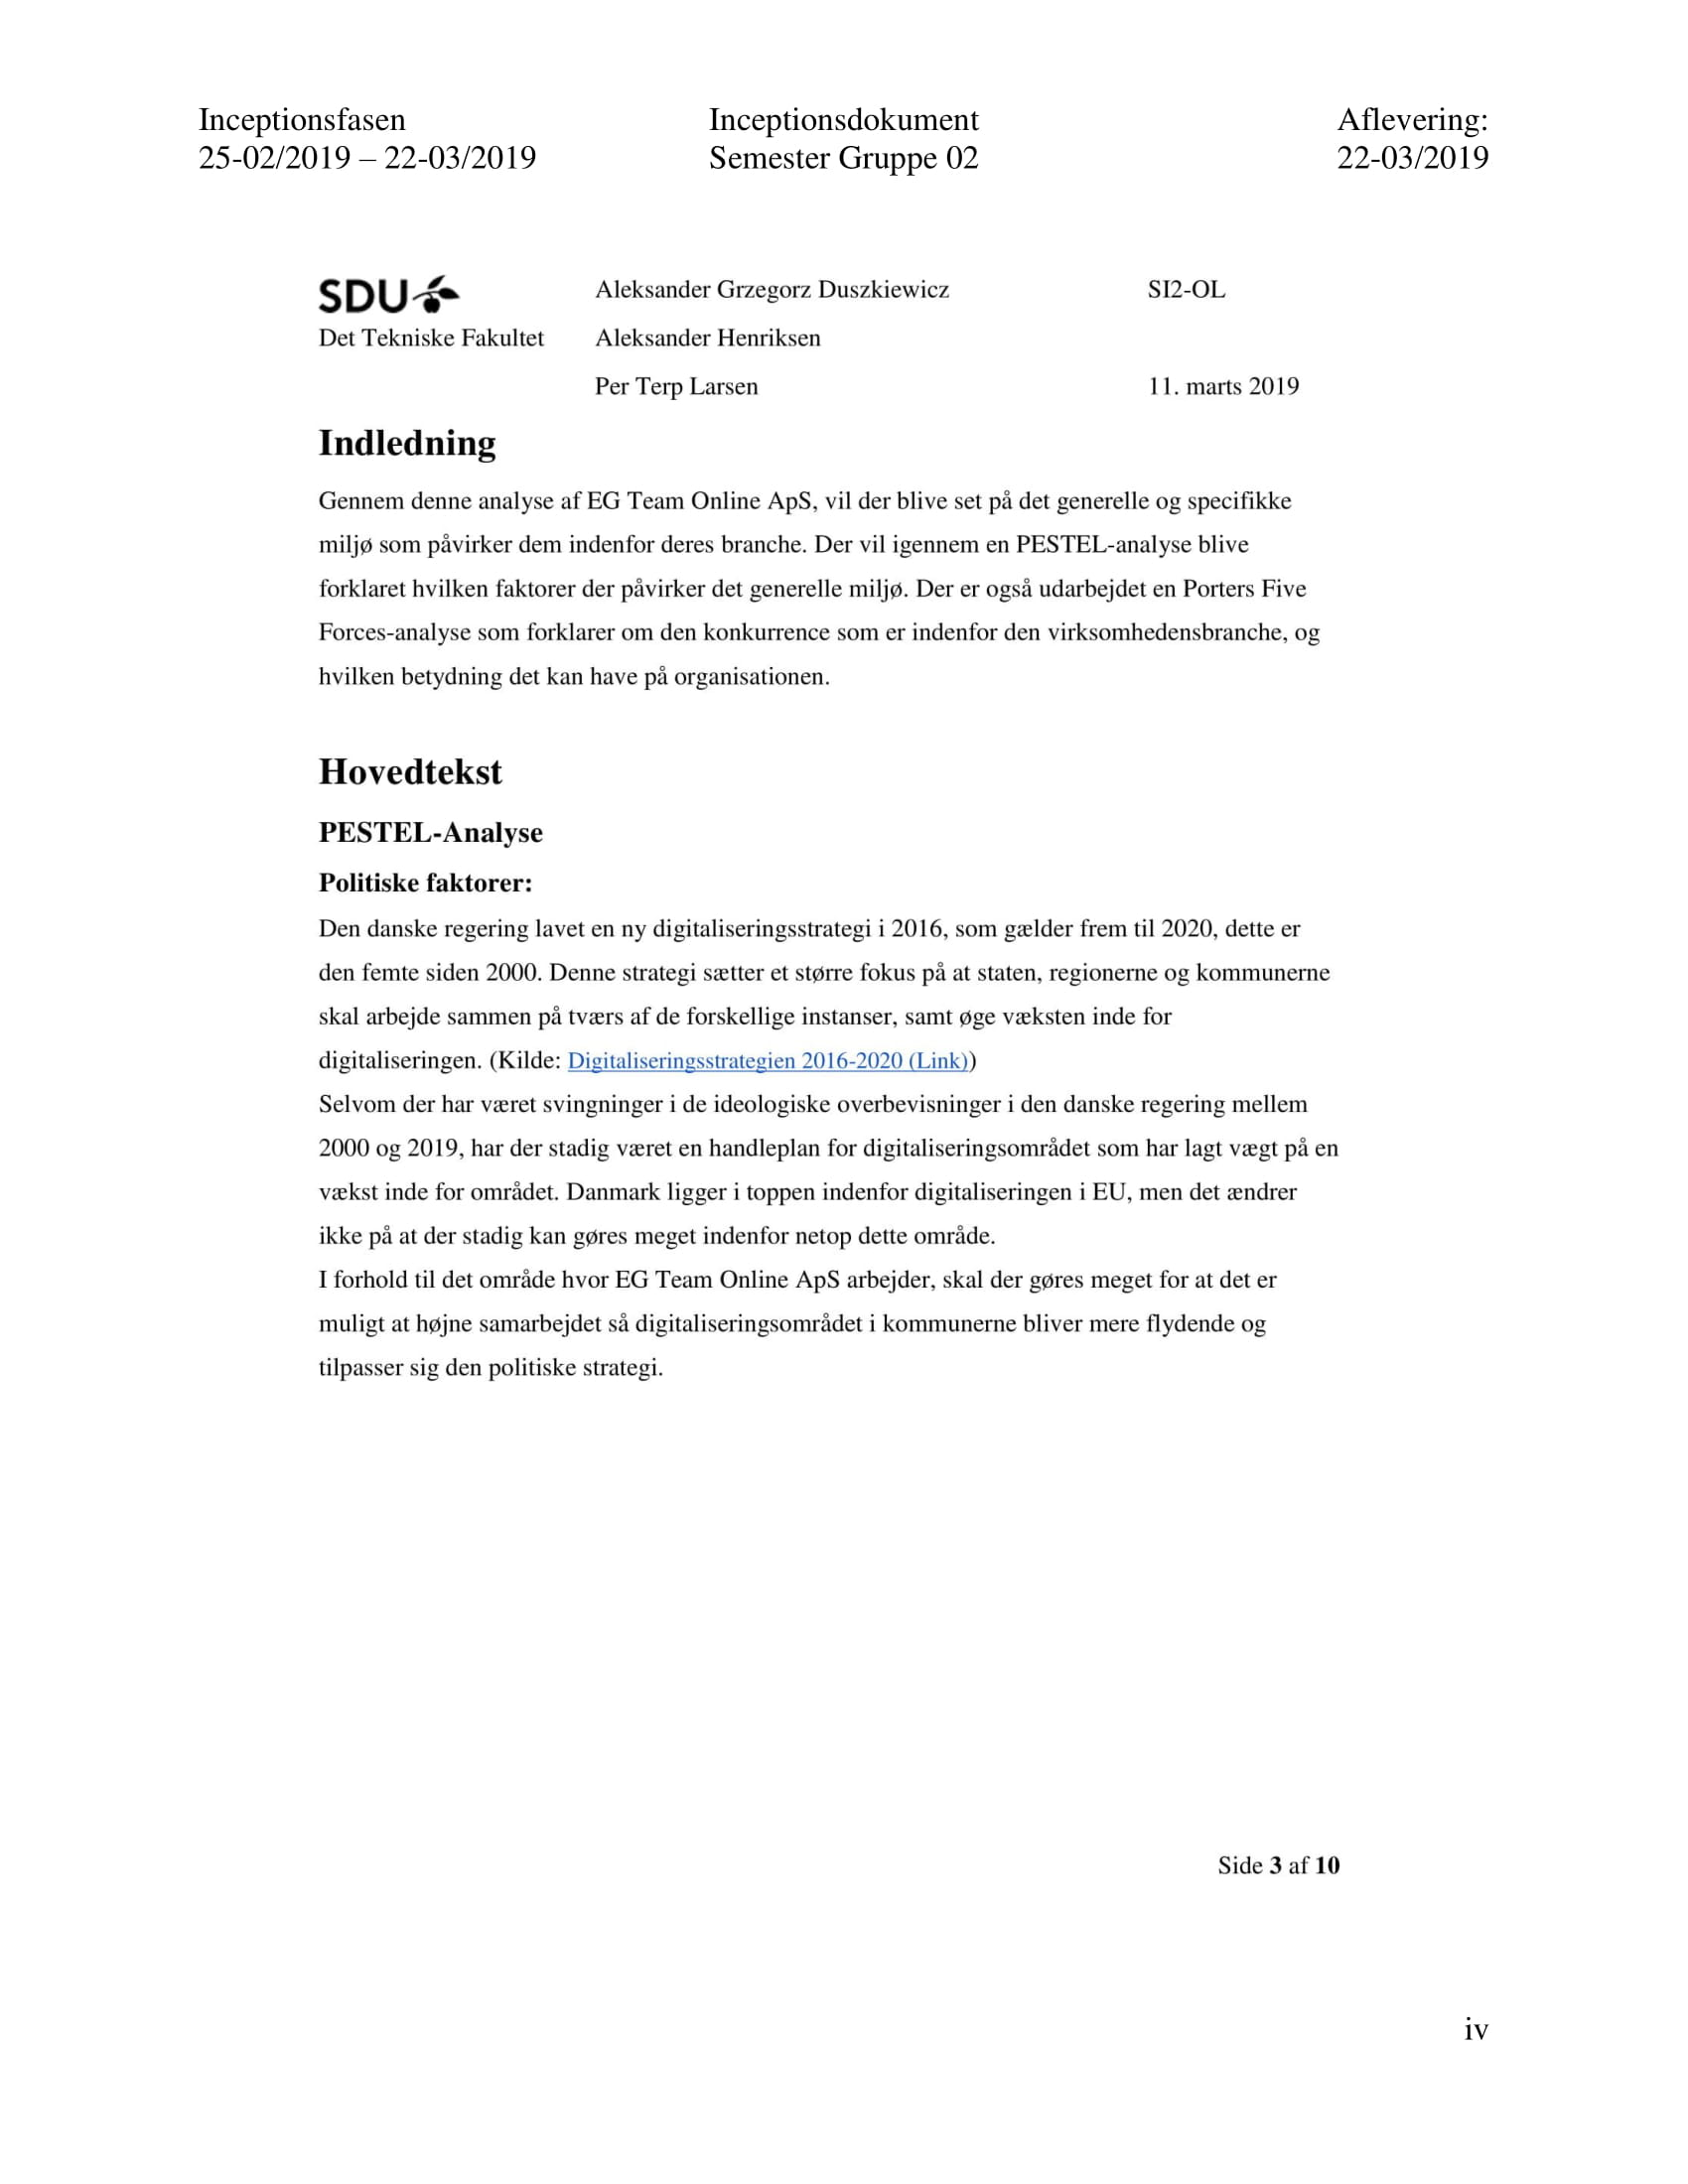
\includegraphics[scale = 0.33]{./PNG/Inceptions/Gruppe 02 + InceptionsDokument-37.jpg} 
\end{figure}

\begin{figure}[hb]
  \includegraphics[scale = 0.33]{./PNG/Inceptions/Gruppe 02 + InceptionsDokument-38.jpg} 
\end{figure}

\begin{figure}[hb]
  \includegraphics[scale = 0.33]{./PNG/Inceptions/Gruppe 02 + InceptionsDokument-39.jpg} 
\end{figure}

\begin{figure}[hb]
  \includegraphics[scale = 0.33]{./PNG/Inceptions/Gruppe 02 + InceptionsDokument-40.jpg} 
\end{figure}

\begin{figure}[hb]
  \includegraphics[scale = 0.33]{./PNG/Inceptions/Gruppe 02 + InceptionsDokument-41.jpg} 
\end{figure}

\begin{figure}[hb]
  \includegraphics[scale = 0.33]{./PNG/Inceptions/Gruppe 02 + InceptionsDokument-42.jpg} 
\end{figure}

\begin{figure}[hb]
  \includegraphics[scale = 0.33]{./PNG/Inceptions/Gruppe 02 + InceptionsDokument-43.jpg} 
\end{figure}

\begin{figure}[hb]
  \includegraphics[scale = 0.33]{./PNG/Inceptions/Gruppe 02 + InceptionsDokument-44.jpg} 
\end{figure}

\begin{figure}[hb]
  \includegraphics[scale = 0.33]{./PNG/Inceptions/Gruppe 02 + InceptionsDokument-45.jpg} 
\end{figure}

\begin{figure}[hb]
  \includegraphics[scale = 0.33]{./PNG/Inceptions/Gruppe 02 + InceptionsDokument-46.jpg} 
\end{figure}

\begin{figure}[hb]
  \includegraphics[scale = 0.33]{./PNG/Inceptions/Gruppe 02 + InceptionsDokument-47.jpg} 
\end{figure}

\begin{figure}[hb]
  \includegraphics[scale = 0.33]{./PNG/Inceptions/Gruppe 02 + InceptionsDokument-48.jpg} 
\end{figure}

\begin{figure}[hb]
  \includegraphics[scale = 0.33]{./PNG/Inceptions/Gruppe 02 + InceptionsDokument-49.jpg} 
\end{figure}

\begin{figure}[hb]
  \includegraphics[scale = 0.33]{./PNG/Inceptions/Gruppe 02 + InceptionsDokument-50.jpg} 
\end{figure}

\begin{figure}[hb]
  \includegraphics[scale = 0.33]{./PNG/Inceptions/Gruppe 02 + InceptionsDokument-51.jpg} 
\end{figure}

\begin{figure}[hb]
  \includegraphics[scale = 0.33]{./PNG/Inceptions/Gruppe 02 + InceptionsDokument-52.jpg} 
\end{figure}

\begin{figure}[hb]
  \includegraphics[scale = 0.33]{./PNG/Inceptions/Gruppe 02 + InceptionsDokument-53.jpg} 
\end{figure}

\section{Rapportkontrolskema}
\begin{center}
\begin{longtable}{|m{3.5cm}|m{10cm}|m{2.5cm}|}
\hline
\multicolumn{3}{|c|}{A. Produktrapport} \\
\hline
Kapitel & krav & opfyldt $+/-$ \\ \hline
Omslag & Indeholder omslaget projekttitel, uddannelsesinstitution, fakultet, institut, uddannelse, semester, kursuskode, projektperiode, vejleder, projektgruppe og projektdeltagere (fornavn, efternavn, sdu-email)? & \\
\hline
Titelblad & (Som omslag ekskl. evt. illustration + evt. kildehenvisning til evt. omslagsillustration. Omslaget kan udgøre både omslag og titelblad. Hvis der medtages selvstændigt titelblad, så er titelbladet rapportens første højre side) & \\
\hline
Resumé & 
Omfatter resuméet:
\begin{itemize}
\item Den behandlede problemstilling - hvad blev der arbejdet med og hvorfor?
\item Fremgangsmåden - anvendte metoder - hvordan blev der arbejdet med det? 
(hvordan angreb I problemet og hvordan realiserede I løsningen (hvem, hvad, hvornår og hvorfor))
\item Hovedresultater og konklusioner  – hvad kom der ud af arbejdet?
\end{itemize}
(max  1 side)& \\
\hline
Forord & Indeholder forord hensigten med rapporten, målgruppe, forhistorie, anerkendelser, afleveringsdato samt underskrifter af alle projektdeltagere? \newline
Bemærk: Projektdeltagernes aktive deltagelse i projektforløbet anerkendes gensidigt ved projektdeltagernes underskrifter i rapporten. & \\
\hline
Indholdsfortegnelse & Er der en samlet indholdsfortegnelse for hele projektrapporten?. (Højst to eller tre niveauer i indholdsfortegnelse) & + \\
\hline
Læsevejledning & Er der en vejledning i, hvordan rapporten kan læses, eksempelvis i form af hvilken rækkefølge afsnittene kan læses i og hvordan sammenhængen er mellem de forskellige dele af rapporten, fx mellem produktrapport og bilag? 
\newline Er rapportens målgruppe beskrevet? & \\
\hline
Redaktionelt & Beskriver redaktionelt skriveprocessen og ansvarsområder i skriveprocessen?\newline
Ansvarsområder kan fx beskrives på fx følgende form: 
\begin{tabular}{|c|c|c|c|}
\hline Afsnit & Ansvarlig & Bidrag fra & Kontrolleret af \\ \hline
Afsnit a & Person a & Person b & Person a,b,c \\ \hline
Afsnit b & Person b & Person a & Person a,b,c \\ \hline
Afsnit c & Person c & Person b & Person a,b,c \\ \hline 
\end{tabular} & \\
\hline
Ordliste & Er der en kort beskrivelse af de fagtermer der bruges gennem rapporten? & \\
\hline 
Indledning & Giver indledningen et overblik over projektet og baggrunden for det? & \\
\hline
& Giver indledningen et resume af den udleverede case? & \\
\hline
& Indeholder indledningen problemformuleringen, jfr. inceptiondokumentet? & \\
\hline
& Beskriver indledningen formålet med projektet? Er formålet i overensstemmelse med hensigten med 2. semester? & \\
\hline 
& Beskriver indledningen målene med projektet? Udtrykker målene specifikke, målbare resultater, jfr. inceptionsdokumentet? Er målene i overensstemmelse med de overordnede mål for 2. semester som udtrykt i studieordningens kap. 9 og de mere specifikke mål for projektet, som udtrykt i fagbeskrivelsen for SI2-PRO? & \\
\hline
Metoder & & \\ \hline
\begin{flushright}
1. Indledning 
\end{flushright}
& Giver indledningen en introduktion til  afsnittet? & \\
\hline
\begin{flushright}
2. Metode
\end{flushright}
&Er metoden i det samlede projekt beskrevet?\newline
Er det beskrevet hvordan UP og Scrum kombineres i projektet, samt hvilke fordele og ulemper der er ved det? & \\
\hline
\begin{flushright}
3. Planlægning
\end{flushright}
& Er planlægningen af elaborationsfasen og de enkelte iterationer beskrevet.\newline
Er backlogs beskrevet?\newline
Er rollefordelingen i projektgruppen beskrevet?\newline
Er ceremonierne beskrevet?\newline
Er scrum-buts beskrevet?\newline
Bygger planen på prioriteringen af kravene efter inceptionsfasen. & \\
\hline
hovedtekst & & \\ \hline
\begin{flushright}
1. Indledning
\end{flushright} & Indeholder indledningen en overordnet introduktion til afsnittet? &\\ \hline
\begin{flushright}
2. Overordnet kravspecifikation (resume, opdateret)
\end{flushright} & Indeholder afsnittet et opdateret resumé  af systemafgrænsningen fra inceptionsdokumentet. & \\ \hline
\begin{flushright}
3. Detaljeret kravspecifikation
\end{flushright} & 
Omfatter den detaljerede kravspecifikation \newline
\begin{enumerate}
\item Detaljeret brugsmønsterdiagram (hvis relevant)
\item Detaljerede brugsmønsterbeskrivelser 
\item Detaljerede beskrivelser af supplerende krav Fx organiseret efter FURPS+
\end{enumerate}
& \\
\hline
\begin{flushright}
4. Analyse
\end{flushright}
& Omfatter afsnittet overvejelser, beslutninger og resultater vedr. \newline
\begin{enumerate}
\item Den statiske side af analysemodel
\item Den dynamiske side af analysemodel
\end{enumerate}
& \\ \hline
\begin{flushright}
5. Design 
\end{flushright}
& Omfatter afsnittet overvejelser, beslutninger og resultater vedr. \newline
\begin{enumerate}
\item Softwarearkitektur
\item Subsystemdesign
\item Den statiske side af designmodel
\item Den dynamiske side af designmodel
\item Design af persistens
\item Databasedesign
\end{enumerate}
& \\ \hline
\begin{flushright}
6. Implementering
\end{flushright} 
& Omfatter afsnittet overvejelser, beslutninger og resultater vedr.  konvertering fra design til kode illustreret gennem udvalgte centrale eksempler, samt andre vigtige implementeringsbeslutninger\newline
Omfatter afsnittet implementering af database. & \\ 
\hline
\begin{flushright}
7. Test
\end{flushright}
& Omfatter afsnittet en beskrivelse af de udførte test samt resultatet af dem. & \\
\hline
& Er der medtaget resultater både fra iteration \# 1 og fra iteration \# 2? & \\ 
\hline
Diskussion &
Omfatter diskussionen hvad der er opnået, og hvad der ikke er opnået i projektet i forhold til det forventede som beskrevet i indledningen. \newline
Hvad er styrkerne og svaghederne ved jeres resultater? \newline
Kunne I have opnået bedre resultater?
& \\ \hline
Konklusion & Opsummerer konklusionen resultaterne og diskussionen af dem og giver det på problemformuleringen?  & \\
\hline
Perspektivering & 
Fremtidigt arbejde: Hvad ville de næste skridt i projektet være, hvis der var mere tid?\newline
Refleksion: Hvordan ville I gribe projektet an, hvis I skulle starte forfra? & \\
\hline
Litteraturliste & 
Er litteratur angivet på en anerkendt form? \newline
Er alle former for litteratur som bøger, artikler og hjemmesider medtaget? \newline
Er der kildehenvisninger i teksten? Materiale som gruppen ikke selv har fremstillet i dette projekt skal være angivet med kilde! \newline
Er alle kildehenvisninger i teksten anført på samme måde? \newline
Er der kildeangivelser på figurer, grafer etc. som projektgruppen ikke selv har frembragt? & \\
\hline
\end{longtable}
\end{center}


\begin{center}
\begin{longtable}{|m{3.5cm}|m{10cm}|m{2.5cm}|}
\hline
\multicolumn{3}{|c|}{B. Procesrapport} \\
\hline
Kapitel & krav & opfyldt $+/-$ \\ \hline
Læring og refleksion & Er der en redegørelse for læring og refleksion? & \\ \hline
Projektarbejdet & Er der en redegørelse for projektarbejdet? Er der en beskrivelse af det faktiske projektforløb, med inddragelse af væsentlige artefakter, som fx sprint backlogs, væsentlige ceremonier, som fx  daily scrum, rollevaretagelse mm? & \\ 
\hline
\begin{flushleft} 
Identifikationg, analyse og bearbejdning af problemer
\end{flushleft}
& Er der en redegørelse for identifikation, analyse og bearbejdning af problemer & \\ 
\hline
Projektforløb & & \\ \hline
\begin{flushleft} 
Formidling og kommunikation
\end{flushleft}
& Er der en redegørelse for formidling og kommunikation & \\ 
\hline
\begin{flushleft} 
Samarbejde i gruppen 
\end{flushleft}
& Er der en redegørelse for samarbejde i gruppen & \\ \hline
\begin{flushleft} 
Samarbejde med vejleder
\end{flushleft}
& Er der en redegørelse for samarbejde med vejleder & \\ \hline

\end{longtable}
\end{center}

\begin{center}
\begin{longtable}{|m{3.5cm}|m{10cm}|m{2.5cm}|}
\hline
\multicolumn{3}{|c|}{C. Kildekode} \\ \hline
Kapitel & krav & opfyldt $+/-$ \\ \hline
\begin{flushleft} 
Oversigt over projektets kildekode
\end{flushleft} 
& Er der en oversigt over projektets kildekode, fx filstruktur eller javadoc? & \\ \hline
\end{longtable}
\end{center}

\begin{center}
\begin{longtable}{|m{3.5cm}|m{10cm}|m{2.5cm}|}
\hline
\multicolumn{3}{|c|}{D. Brugervejledning} \\ \hline
Kapitel & krav & opfyldt $+/-$ \\ \hline
Brugervejledning & Er der en kortfattet brugervejledning? & \\ \hline

\end{longtable}
\end{center}

\begin{center}
\begin{longtable}{|m{3.5cm}|m{10cm}|m{2.5cm}|}
\hline
\multicolumn{3}{|c|}{E. Projektlog} \\ \hline
Kapitel & krav & opfyldt $+/-$ \\ \hline
Projektlog & Er der en adresse på og et link til projektloggen i Github & \\ \hline
\end{longtable}
\end{center}

\begin{center}
\begin{longtable}{|m{3.5cm}|m{10cm}|m{2.5cm}|}
\hline
\multicolumn{3}{|c|}{F. Interne bilag} \\ \hline
Kapitel & krav & opfyldt $+/-$ \\ \hline
Projektgrundlag & Er projektgrundlaget medtaget? & \\ \hline
Rapportkontrolskema & Er der et udfyldt rapportkontrolskemaet & \\ \hline
Andet & Er der andre relevante interne bilag, dvs. materialer produceret af gruppen selv? & \\ \hline
\end{longtable}
\end{center}

\begin{center}
\begin{longtable}{|m{3.5cm}|m{10cm}|m{2.5cm}|}
\hline
\multicolumn{3}{|c|}{G. Eksterne bilag} \\ \hline
Kapitel & krav & opfyldt $+/-$ \\ \hline
Eksterne bilag & 
Er der medtaget relevante eksterne bilag, dvs. materialer som gruppen ikke selv har produceret med som er nødvendige for at kunne læse rapporten? & \\ 
\hline
\end{longtable}
\end{center}

\begin{center}
\begin{longtable}{|m{3.5cm}|m{10cm}|m{2.5cm}|}
\hline
\multicolumn{3}{|c|}{H. Rapporttekniske elementer} \\ \hline
Kapitel & krav & opfyldt $+/-$ \\ \hline
Layout & Er der anvendt samme layout i alle kapitler? \newline
Er layout overskueligt/harmonisk? & \\ \hline
Sprog & Er rapporten skrevet i en neutral sprogtone? \newline
Er sproget let læseligt og flydende? \newline
Er der udført stavekontrol og kontrol af tegnsætning? & \\ \hline
Sidenummerering & Er der korrekt og konsistent sidenummerering i rapporten? & \\ 
\hline
Figurer/diagrammer & Er alle figurer konsekvent nummererede? \newline
Er der figurtitel og figurtekst til alle figurer? \newline
Er figurtitler og figurtekster dækkende og afklarende? \newline
Er figurerne tydelige og læsbare? \newline
Er figurerne informationsgivende og i den rette sammenhæng?
& \\ \hline
Tabeller & 
Er alle tabeller konsekvent nummererede? \newline
Er der en forklarende tabeltekst til alle tabeller? \newline
Er alle søjler og rækker forsynet med parametre? \newline
Er der enheder på alle relevante rækker og søjler? 
& \\ \hline
\begin{flushleft} 
Sporbarhed af begreber 
\end{flushleft}
& Er der en konsekvent brug af samme betegnelse for et givet begreb igennem rapporten? & \\ \hline




\end{longtable}
\end{center}
\newpage
\section{Diverse interne materialer}







\end{document}